% This thesis template has been put together and edited by Diego Pizzocaro
% It's a collection/edit of files produced by Frank C Langbein for his PhD thesis
% and then edited by Ahmed Alazzawi, Hmood Al Dossari, Manar I. Hosny, H.Z. Al-Dossari 
% and kindly shared by them.
%
% Following, the original GNU license chosen by Frank C Langbein, 
% which is the same license for distributing this package.
%
% beautification.tex -- Beautification of Reverse Engineered Geometric Models
%% PhD Thesis by Frank C. Langbein%
% Maintainer: Frank C. Langbein <frank@langbein.org>
% Version: 1.0
% Copyright (c) 2003 Frank C Langbein.
% Permission is granted to copy, distribute and/or modify this document
% under the terms of the GNU Free Documentation License, Version 1.2 or
% any later version published by the Free Software Foundation; with no
% Invariant Sections, no Front-Cover Texts, and no Back-Cover Texts. A
% copy of the license is included in the section entitled "GNU Free
% Documentation License".
%


\documentclass[a4paper,oneside,onecolumn,openright,12pt]{book}


\makeatletter
% Copy pasted junk

\newcommand{\green}[1]{\textcolor{green}{#1}}


%Graphics
%\usepackage{graphicx}
% Langbein added these - Tom
\usepackage{caption}
\usepackage{footmisc}
\usepackage{paralist}
\usepackage{array}
\usepackage{epsf}
\usepackage{amsmath}
\usepackage{rotating}
\usepackage{listings}
\usepackage{varwidth}
\usepackage{adjustbox}
\usepackage{tabularx}
\usepackage{listings}
\usepackage{amsthm}
\usepackage{longtable}
\usepackage{afterpage}
\usepackage{subfig}
%\usepackage{algorithm}
%\usepackage{rotating}
%\usepackage{amssymb}
\usepackage{multibib}
\usepackage{booktabs}
% Fonts, encoding, etc.
\usepackage{type1cm}
\usepackage[latin1]{inputenc}
\usepackage[british]{babel}
\usepackage[T1]{fontenc}
\usepackage{times}
\usepackage{hyperref}
\usepackage[all]{hypcap}
\usepackage{longtable}
%\usepackage{algorithm}
\usepackage[noend]{algorithmic}
%\usepackage{rotating}
\usepackage{multirow}
\usepackage{lscape}
\usepackage{float}
%\usepackage{subfigure}
% Line spacing
\def\baselinestretch{1.5}
\parindent0cm
\parskip1.5ex\@plus.7ex\@minus.1ex\relax
\lstset{
	basicstyle=\ttfamily,
	columns=fullflexible,
	keepspaces=true,
}

%Acronyms
 \usepackage{acronym}
 %Inline lists
 \usepackage{paralist}

% Page dimensions
\usepackage{vmargin}
\setpapersize{A4}
\setmarginsrb{25mm}{20mm}{25mm}{10mm}{14.5pt}{8mm}{0pt}{11mm}

% Footer and header
\usepackage{afterpage}
\usepackage{fancyhdr}
\pagestyle{fancy}
\fancyhead{}
\fancyhead[LE,RO]{\thepage}
\fancyhead[LO,RE]{\slshape \leftmark}
\fancyfoot{}
\renewcommand{\chaptermark}[1]{}
\renewcommand{\sectionmark}[1]%
             {\markboth{\thesection\ #1}{\thesection\ #1}}
\renewcommand{\subsectionmark}[1]{}
\fancypagestyle{plain}{%
  \fancyhead{}
  \fancyhead[LE,RO]{\thepage}
  \fancyfoot{}
  \renewcommand{\headrulewidth}{.6pt}
}

% Chapter
\def\@makechapterhead#1{%
  \ \\[-35.5pt]\hbox to \textwidth {%
    \hfill {\vbox{\hbox{\rule[5pt]{140pt}{4pt}}%
        \hbox to 140pt {\hfill\huge\bfseries\slshape \@chapapp\space\thechapter\/}}}}%
  \vskip55\p@%
  {\parindent \z@ \raggedright \normalfont%
    \interlinepenalty\@M%
    \Huge \bfseries #1\par\nobreak%
    \vskip 45\p@%
  }}
\def\@chapter[#1]#2{\ifnum \c@secnumdepth >\m@ne
                       \if@mainmatter
                         \refstepcounter{chapter}%
                         \typeout{\@chapapp\space\thechapter.}%
                         \addcontentsline{toc}{chapter}%
                                   {\protect\numberline{\thechapter}#1}%
                       \else
                         \addcontentsline{toc}{chapter}{#1}%
                       \fi
                    \else
                      \addcontentsline{toc}{chapter}{#1}%
                    \fi
                    \chaptermark{#1}%
                    \addtocontents{lof}{\protect\addvspace{10\p@}}%
                    \addtocontents{lot}{\protect\addvspace{10\p@}}%
                    \addtocontents{loa}{\protect\addvspace{10\p@}}%
                    \if@twocolumn
                      \@topnewpage[\@makechapterhead{#2}]%
                    \else
                      \@makechapterhead{#2}%
                      \@afterheading
                    \fi}
\def\@schapter#1{\addcontentsline{toc}{chapter}{#1}%
                 \markboth{#1}{#1}%
                 \addtocontents{lof}{\protect\addvspace{10\p@}}%
                 \addtocontents{lot}{\protect\addvspace{10\p@}}%
                 \addtocontents{loa}{\protect\addvspace{10\p@}}%
                 \if@twocolumn%
                    \@topnewpage[\@makeschapterhead{#1}]%
                 \else%
                    \@makeschapterhead{#1}%
                    \@afterheading%
                 \fi}
\def\@makeschapterhead#1{%
  \ \\[-35.5pt]\hbox to \textwidth {%
    \hfill {\vbox{\hbox{\rule[5pt]{140pt}{0pt}\rule[5pt]{0pt}{4pt}}%
        \hbox to 140pt {\hfill\huge\bfseries\slshape \ \/}}}}%
  \vskip55\p@%
  {\parindent \z@ \raggedright \normalfont%
    \interlinepenalty\@M%
    \Huge \bfseries  #1\par\nobreak%
    \vskip 45\p@%
  }}

% Table of contents
\def\contentsname{Contents}
\renewcommand\tableofcontents{%
    \if@twocolumn%
      \@restonecoltrue\onecolumn%
    \else%
      \@restonecolfalse%
    \fi%
    \chapter*{\contentsname}%
    \@starttoc{toc}%
    \if@restonecol\twocolumn\fi%
    }

% Bibliography
\renewenvironment{thebibliography}[1]
     {\chapter*{\bibname}%
      \list{\@biblabel{\@arabic\c@enumiv}}%
           {\settowidth\labelwidth{\@biblabel{#1}}%
            \leftmargin\labelwidth
            \advance\leftmargin\labelsep
            \@openbib@code
            \usecounter{enumiv}%
            \let\p@enumiv\@empty
            \renewcommand\theenumiv{\@arabic\c@enumiv}}%
      \sloppy
      \clubpenalty4000
      \@clubpenalty \clubpenalty
      \widowpenalty4000%
      \sfcode`\.\@m}
     {\def\@noitemerr
       {\@latex@warning{Empty `thebibliography' environment}}%
      \endlist}

% Floats
\long\def\@makecaption#1#2{%
  \vskip\abovecaptionskip
  \sbox\@tempboxa{\textbf{#1: #2}}%
  \ifdim \wd\@tempboxa >\hsize
    \textbf{#1: #2.}\par
  \else
    \global \@minipagefalse
    \hb@xt@\hsize{\hfil\box\@tempboxa\hfil}%
  \fi
  \vskip\belowcaptionskip}
\renewcommand{\topfraction}{0.9}
\renewcommand{\textfraction}{0.1}
\renewcommand{\floatpagefraction}{0.9}

% Tables
\usepackage{dcolumn}
\usepackage{hhline}

% Graphics
\usepackage[dvips]{graphicx}
\usepackage{rotating}
\usepackage{psfrag}
\usepackage{epic}
\usepackage{tabularx}
\usepackage{eepic}

% Algorithm environment
\newcounter{algorithm}[chapter]
\renewcommand{\thealgorithm}{\thechapter.\@arabic\c@algorithm}
\def\fps@algorithm{t}
\def\ftype@algorithm{1}
\def\ext@algorithm{loa}
\def\fnum@algorithm{Algorithm~\thealgorithm}
\newenvironment{algorithm}{\@float{algorithm}}{\end@float}
\newenvironment{algorithm*}{\@dblfloat{algorithm}}{\end@dblfloat}
\newenvironment{alevel}%
   {\begin{list}{}{%
      \setlength{\topsep}{0pt}%
      \setlength{\parskip}{0pt}%
      \setlength{\partopsep}{0pt}%
      \setlength{\parsep}{0pt}%
      \setlength{\itemsep}{0pt}}}%
   {\end{list}}
\newcommand\listalgorithmsname{List of Algorithms}
\newcommand\listofalgorithms{%
    \if@twocolumn
      \@restonecoltrue\onecolumn
    \else
      \@restonecolfalse
    \fi
    \chapter*{\listalgorithmsname}%
      \@mkboth{\listalgorithmsname}{\listalgorithmsname}%
    \@starttoc{loa}%
    \if@restonecol\twocolumn\fi
    }
\newcommand*\l@algorithm{\@dottedtocline{1}{1.5em}{2.3em}}

% List of figures and tables
\renewcommand\listoffigures{%
    \if@twocolumn
      \@restonecoltrue\onecolumn
    \else
      \@restonecolfalse
    \fi
    \chapter*{\listfigurename}%
      \@mkboth{\listfigurename}{\listfigurename}%
    \@starttoc{lof}%
    \if@restonecol\twocolumn\fi
    }
\renewcommand\listoftables{%
    \if@twocolumn
      \@restonecoltrue\onecolumn
    \else
      \@restonecolfalse
    \fi
    \chapter*{\listtablename}%
      \@mkboth{\listtablename}{\listtablename}%
    \@starttoc{lot}%
    \if@restonecol\twocolumn\fi
    }

% Math symbols, fonts, etc.
\usepackage{amsmath}
\usepackage{amsfonts}
\usepackage{amssymb}

\newcommand{\N}{\mathbb{N}}
\newcommand{\Z}{\mathbb{Z}}
\newcommand{\Q}{\mathbb{Q}}
\newcommand{\R}{\mathbb{R}}
\newcommand{\C}{\mathbb{C}}
\renewcommand{\S}{\mathbb{S}}
\renewcommand{\P}{\mathbb{P}}
\newcommand{\E}{\mathbb{E}}

\newcommand{\Cf}{\mathfrak{C}}
\newcommand{\Pf}{\mathfrak{P}}

\DeclareMathOperator{\sign}{sign}
\DeclareMathOperator{\avg}{avg}
\DeclareMathOperator{\floor}{floor}
\DeclareMathOperator{\ceil}{ceil}
\DeclareMathOperator{\round}{round}

\providecommand{\abs}[1]{\lvert#1\rvert}
\providecommand{\absd}[1]{\left\lvert#1\right\rvert}
\providecommand{\card}[1]{\lvert#1\rvert}
\providecommand{\norm}[1]{\lVert#1\rVert}

% URLs
\usepackage{url}
%% Define a new 'leo' style for the package that will use a smaller font.
\makeatletter
\def\url@leostyle{%
  \@ifundefined{selectfont}{\def\UrlFont{\sf}}{\def\UrlFont{\footnotesize\ttfamily}}}
\makeatother
%% Now actually use the newly defined style.
\urlstyle{leo}



\makeatother


\begin{document}


\frontmatter


\begin{titlepage}

\begin{center}
\vspace*{3ex}
\textbf{\Huge Disentangling \new{L}ow-\new{D}imensional \new{V}ector \new{S}pace \new{R}epresentations of \new{T}ext \new{D}ocuments}\\[2ex]
%\textbf{\Huge Title line 2}\\[12ex]
\textbf{\large A thesis submitted in partial fulfilment}\\[1ex]
\textbf{\large of the requirement for the degree of Doctor of
  Philosophy}\\[16ex]
\textbf{\LARGE Thomas J. Ager}\\
\vfill
\textbf{\LARGE January 2020}\\
\vfill
\textbf{\LARGE Cardiff University}\\[1ex]
\textbf{\LARGE School of Computer Science \& Informatics}\\[4ex]
\end{center}

\end{titlepage}
\newpage\thispagestyle{empty}\cleardoublepage


\thispagestyle{plain}

\textbf{\large Declaration}

This thesis is the result of my own independent work, except where otherwise stated,
and the views expressed are my own. Other sources are acknowledged by explicit references.
The thesis has not been edited by a third party beyond what is permitted by
Cardiff University's Use of Third Party Editors by Research Degree Students Procedure.\\[2ex]
Signed \dotfill \ (candidate) \hspace*{10em}\\[1ex]
Date\ \ \ \ \ \dotfill \hspace*{18em}

\vfill

\vfill

\textbf{\large Statement 1}

This thesis is being submitted in partial fulfilment of the requirements for the degree of PhD.\\[2ex]
Signed \dotfill \ (candidate) \hspace*{10em}\\[1ex]
Date\ \ \ \ \ \dotfill \hspace*{18em}

\textbf{\large Statement 2}

This thesis is the result of my own independent work/investigation,
except where otherwise stated. Other sources are acknowledged by
explicit references.\\[2ex]
Signed \dotfill \ (candidate) \hspace*{10em}\\[1ex]
Date\ \ \ \ \ \dotfill \hspace*{18em}

\vfill

\textbf{\large Statement 3}

I hereby give consent for my thesis, if accepted, to be available for photocopying and for inter-library loan,
 and for the title and summary to be made available to outside organisations.\\[2ex]
Signed \dotfill \ (candidate) \hspace*{10em}\\[1ex]
Date\ \ \ \ \ \dotfill \hspace*{18em}

\vfill

\vspace*{3ex}

\textbf{\large Word Count}  \ \ \ \ \dotfill \hspace*{18em}

(Excluding Abstract, acknowledgements, declarations, contents pages, appendices, tables,
diagrams and figures, references, bibliography, footnotes and endnotes)



\ \vspace*{1.11cm}
\markboth{Dedication}{}
\begin{flushright}
\textbf{\large To my parents.}\\
\textbf{\large for their invaluable and unwavering support.}
\end{flushright}
\newpage
\markboth{}{}
\cleardoublepage


\chapter*{Abstract}

%%%%%%%%%%%%%%%%% OLD WORK

%NESY 
%Vector space embeddings can be used as a tool for learning semantic relationships from unstructured text documents. Among others, earlier work has shown how in a vector space of entities (e.g.\ different movies) fine-grained semantic relationships can be identified with directions (e.g.\ more violent than).

%IJCAI 
%In many applications, it is important for classification models to be interpretable. Unfortunately, however, prominent While dimensionality reduction methods could be used in principle, the resulting dimensions would typically not be interpretable. To address this shortcoming, we propose a method to learn interpretable features from a given low-dimensional vector space representation.

%CONLL
%In this paper we consider semantic spaces consisting of objects from some particular domain (e.g.\ IMDB movie reviews). and 

%%%%%%%%%%%%%%%%% OLD WORK


% General problem introduction, why it matters, what past work did, what the results will achieve

% Most vector spaces are entangled


% By the way, if you use the word disentangled in the title of your thesis, you should explain this term in the abstract.

% Broader context

%This thesis is concerned with vector space representations of  documents in a given domain (e.g.\ movies in a domain of movie reviews). Such representations are often learned from text documents that describe these entities. 
In contrast to traditional document representations such as bags-of-words, the kind of vector space representations that are currently most popular tend to be lower-dimensional. This has important advantages, e.g.\ making the representation of a given document less dependent on the exact words that are used. However, this also comes at an important cost, namely that the representation is  "entangled", meaning that the features of the representation are not individually meaningful or interpretable. The main aim of this thesis is to address this problem  by disentangling   vector spaces into representations that are composed of individual, important and meaningful features in the given domain. For instance, in the domain of IMDB movie reviews, where each document is a review, the disentangled feature representation would be separated into features that describe how ("Scary", "Romantic", ..., "Comedic"),  the  movie is. This thesis builds on an initial approach introduced by  Derrac \cite{Derrac2015}, where it was  observed that low-dimensional vector space representations of documents  often model important features of the domain as directions. The method begins by obtaining direction vectors for all terms  using a linear classifier to find a hyper-plane that separates documents that have a term and do not have a term. Then, from each hyper-plane the orthogonal vector is taken as a direction that goes from documents that are least related to the word (as they are furthest from the hyper-plane on the negative side) to documents that are most related to it (as they are furthest from the hyper-plane on the positive side). However, while some words describe semantically important features, others may be completely irrelevant. The importance of these terms is determined by how well the linear classifier performs on a standard classification metric,  which approximates how linearly separable the documents are that contain the term in the vector space. The most important terms are selected, and documents are ranked on these directions by calculating the dot product between the orthogonal vector to the hyper-plane and each document vector. This results in  a value that corresponds to how  far up documents are on the direction, enabling    documents to be ranked on how much they \textit{have} a particular meaningful feature,  e.g.\ movies can be ranked on how "Scary" they are. %In terms of application, a representation like this can be used in entity oriented search engines, recommendation systems, among others, or perhaps even be used as input to a simple classifier as an alternative to a hard to decipher  neural networks. 

% Contribution 1

The work by Derrac \cite{Derrac2015} obtained semantic features from Multi-Dimensional Scaling (MDS) document embeddings and validated their work by classifying documents using a rule-based classifier (FOIL), resulting in rules of the form "\textbf{IF} \textit{x} is more scary than most horror films \textbf{THEN} \textit{x} is a horror film.". The first main contribution of this thesis is a deeper investigation and improvement of this method, in particular by  experimentally validating that the  features derived from the initial embeddings are clear and semantically meaningful across a variety of unsupervised document embedding models and domains. Furthermore, variants of the method are introduced that are shown to improve  performance. We also introduce the use of low-depth decision trees to evaluate the quality of the disentangled representations in a clear quantitative way.

% Contribution 2

Neural network architectures have advanced to  state-of-the-art  in many tasks. The second main contribution of the work  follows the idea that the  hidden layers of a neural network can be viewed as document embeddings. Specifically, semantic features are derived from the  hidden layers of neural networks. In particular, a qualitative analysis of two kinds of neural networks is conducted, feed-forward networks and stacked auto-encoders. Auto-encoders are  stacked by using their hidden-layer as the input  to another auto-encoder. Characteristics of  learned feed-forward networks are identified. We find in particular that  they can learn higher-quality representations of  features that are relevant to the considered classification problem. In the case of auto-encoders, it is found  that as  auto-encoders are  stacked, increasingly abstract features can be derived from them. For example, in the initial auto-encoder layers, features like "Horror" and "Comedy" can be separated well by the linear classifier, meanwhile in the latter layers features like "society" and "relationships" are easy to separate. After identifying directions that model important features of documents in each stacked auto-encoder, symbolic rules are induced that relate specific features to more general ones. These rules are interesting, as they can clarify the nature of the transformations that are learned by the neural network, for example:

\begin{align}\label{rule1}\texttt{IF Emotions  AND  Journey THEN Adventure}\end{align} 

% Contribution 3

 In addition to introducing variants of the method in \cite{Derrac2015}, this thesis also introduces an additional post-processing step for improving disentangled feature representations by fine-tuning the original embedding to prioritize faithfully modelled directions. Methods for learning document embeddings  are mostly aimed at modelling similarity. It is found  that there is an inherent trade-off between capturing similarity and faithfully modelling features as directions. Following this observation, a simple method to fine-tune  document embeddings is proposed, with the aim of improving the quality of the feature directions obtained from them. Crucially, this  method is also fully unsupervised, requiring only a bag-of-words representation of the objects as input.  In particular,  clusters of terms are identified that refer to semantically meaning and important features of the considered domain, and a simple neural network model is used to learn a new representation in which each of these features is more faithfully modelled as a direction. It is found that in most cases this method improves the ranking of documents, and results in increased performance when disentangled feature representations are used as input to classifiers. %As in Chapter \ref {ch3}, the usefulness of this approach is validated using low-depth decision trees, where it is found that in most cases performance improves.


%The objective of this thesis is to improve how such semantically meaningful feature directions can be learned from a given  document embedding.  This thesis concerns itself with application of this methodology to a variety of document embeddings. These semantic features are beneficial for a variety of purposes,  One important examples is the fact that they provide a useful inductive bias.  they may provide insight into what the neural network is doing correctly or incorrectly in its learning process. 

 %The how semantic these features are is evaluated using a document classification task that classifies decision trees with a limited depth. This limitation verifies that the feature representation has captured features that correspond to domain knowledge, as if the classifier can perform well with a low amount of features those features must be semantic. 



% Paragraph focusing on how methods can be useful for your applications

Overall, this thesis quantitatively and qualitatively validates  that disentangled feature representations of meaningful features can be derived from low-dimensional vector spaces of documents, across a variety of domains and document embedding models.  New variants of the method introduced by Derrac \cite{Derrac2015} are evaluated and found to be effective. Neural networks are investigated, and in the case of  stacked auto-encoders,  features become more abstract as auto-encoders are stacked, and a method that links specific features to more general ones is introduced. In the case of feed-forward networks, a variety of interesting characteristics are observed, in particular that feed-forward networks make features that are more relevant to the task more separable. Finally, a new method is introduced to fine-tune existing document embeddings such that their features are more meaningful. 



%This won't be clear, as you haven't actually explained that the semantic features allow you to derive a more interpretable, feature-based representation of the entities.




%This sentence is not clear. I think you are talking about existing approaches to learn disentangled neural network representations (like InfoGAN), but that won't be clear to the reader + probably this is too much detail for the abstract anyway. 

% features like these are usually obtained by using a specialized learning procedure, e.g.\ by enforcing sparsity constraints or orthogonality between features, and learned from the original text data.

 

%Can this method be applied to a variety of representations?
%Can this method be applied to more domains?
%Does this method result in a representation of clear semantic features?
%Can these semantic features be used to form a useful alternative representation?
%Are the features meaningful qualitatively in a variety of domains and for a variety of representations?

%The work in Chapter \ref{ch3} addresses these questions, and introduces variants to their method that result in  better performance on tasks.

%There are a variety of approaches to obtaining vector space representations where features are clear and semantic. 

%simple models such as (small) decision trees cannot readily be applied to text documents due to the size of the underlying feature space. 
 

  





% Disentanglement and why it matters

% Existing disentanglement methods and why they dont fit the gap

% What we actually did to solve this problem 1st chapter

% What the results were 1st chapter

% What we did 2nd

% Results 2nd

% What we did 3rd

% Results 3rd

% Overall conclusions

%Vector space representations of documents can be re-organized  such that their dimensions correspond to clear semantic features. Furthermore, these disentangled representations can be used to provide a useful inductive bias to classifiers, and as the features are disentangled, they can be used to qualitatively investigate the hidden layers of neural networks to gain valuable insights into how they represent documents. 
%\def\baselinestretch{1}\normalfont

\def\baselinestretch{1.5}\normalfont


\chapter*{Acknowledgements}

It has been a long journey from the start of this PhD to the end of it, and I owe almost all of my success to my supervisor Steven Schockaert, and my unofficial co-supervisor Ondrej Kuzelka. I would like to thank them especially for all their guidance and their many ideas about the work undertaken in the thesis.

I would also like to thank my colleagues at Cardiff University, who provided a community to engage with when I needed an audience for my presentations, or to discuss my thoughts about the work. It is certainly in large part thanks to them that I was able to be where I am today.

My deepest thanks go to my parents, who were able to support me through the final years of my PhD. Finally I thank God, who guided me when I needed it most.

\tableofcontents

\newpage
\chapter*{List of Publications}

The work introduced in this thesis is based on the following publications.

\begin{itemize} 

\item % your publication goes here

\item % your publication goes here

\end{itemize}

\listoffigures

\listoftables

%\listofalgorithms

%

\chapter*{List of Publications} 
\begin{acronym}
\acro{ML}{Machine Learning}
\acro{NLP}{Natural Language Processing}
\acro{NDCG}{Normalized Discounted Cumulative Gain}
  \begin{enumerate}
	\item \bibentry{Ager2012b}
	\item \bibentry{Ager2016}
\end{enumerate}
% to use in the thesis, use: \ac{GPS}
% more goes here.
\end{acronym}



\mainmatter
%begin each chapter chapter1.tex by \Chapter{chapter1}, for example, then the sections and so on...
\chapter{Introduction}\label{ch1}


%%%% Currently

% Rewrote introduction based on talk with steven
%%% Neeed to
% Rewrite hypothesis
% Edit and reform paragraphs of introductory text so that the story is clear, makes sense and has references



%Introduction+conclusion are shorter chapters

%Introduction
%Hypothesis
%research questions
%context
%Summary of the contributions
%Good to introduce gently but research questions can be fine
%Doesn't have to be accessible to the man on the street, need computer science background, vector spaces are included in that, so are decision trees and neural networks, if it's borderline reference background

%%Conclusion revisits research questions, provides the answer not just a summary

%%%%% INTRODUCTION

% There is a lot of data, and a lot of good applications of machine-learning using that data




%!!!!!!!!!!!!!!! NEW INTRO


%  There is a lot of data available, and even more becoming so, so machine-learning that  leverages this data are getting top performance on a lot of tasks.
% Neural networks are not interpretable, Interpretable classifiers are useful because they can drive engagement, increase stakeholder buy in, inform model creators of errors or ways to improve the model, provide insight
% A successful interpretable classifier 1. Uses features that correspond to key domain concepts, and 2. Explains what these concepts represent, as well as the decision made with these concepts 
% we aim to satisfy the first objective, but are not interested in obtaining labels or explanations based on these labels. So, we obtain features that correspond to meaningful and specific concepts that are relevant to classifying key domain tasks For example, when classifying "horror" a good feature would be how "bloody" the movie is., 
% In particular, this work investigates interpretable classifiers for document classification. For example, genres in a domain of movie reviews.
%% Machine learning uses spatial representations of meaning, and neural networks can be seen as constructing such a spatial representation of meaning. 
%This thesis focuses on transforming vector space representations into semantic features in an unsupervised way.    These are obtained from stevens and derrac's method, and are used as directions,  they have previously been found to be   suitable for different applications, like a recommendation system where you can choose something that's "more bloody"



% Move disentanglement to background?, defining disentanglement paper

%\hmark{Typically, to obtain a representation that represents meaningful aspects of the domain, a low-dimensional vector space representation is induced. However, in these representations the features do not correspond to meaningful aspects, but rather this meaning is represented spatially.}   %The problem with these vector spaces is that despite the fact that these representations clearly capture meaning in a non-trivial way,  their features do not typically have any particular meaning. %Ideally, a representation  of documents   is flexible in the information it can represent, and is learned from a large amount of data. To do this, typically Low-dimensional vector space embeddings of documents represent semantic meaning spatially.

% Machine-learning methods can achieve strong results, but are not interpretable.


%  There is a lot of data available, and even more becoming so, so machine-learning that  leverages this data are getting top performance on a lot of tasks.
%  This is in-part thanks to the availability of  text data on the internet, as  social media sites  like Facebook and  Twitter, \hmark{p}roduct and movie review sites like IMDB and Amazon and content-aggregation sites like Reddit have become immensely popular. % , or text classification tasks . \hmark{Some examples of these text classification tasks are} and text classification tasks \cite{Burel2018, Aldarwish2017, Burel2018}. e.g.\  identifying if social media posts or product reviews have a positive or negative sentiment,  identifying social media posts  that are useful to crisis responders during crises, or  predicting depression in social media users. 

% Neural networks are not interpretable, Interpretable classifiers are useful because they can drive engagement, increase stakeholder buy in, inform model creators of errors or ways to improve the model, provide insight
\hmark{In recent years, machine learning models  have  achieved state-of-the-art results on most natural language processing tasks\footnote{https://github.com/sebastianruder/NLP-progress} such as machine translation, \cite{Wu} question answering  \cite{Fisch2016}, and document classification \cite{Yang2019}. % in part thanks to the ability of these models to process  large amounts of unstructured text data made widely available by the internet.
Although these methods perform well, they are typically not interpretable. As machine learning has extended into  real-world domains like medicine and policing, concerns of safety \cite{Amodei2016} and fairness \cite{Mehrabi2019} have brought  the  legality and risk of implementing systems that are not interpretable   to the attention of lawmakers. The European Union introduced  a legal "Right to explanation" in 2018   \cite{Goodman2016}, requiring that machine learning models must be able to explain why they have made a decision about a person. }
%A variety of solutions have Solutions such as explaining machine-learning models after they have been learned have been suggested, as well as making transparent machine-learning models that can be understood by inspection \cite{Gilpina}. 

% A successful interpretable classifier 1. Uses features that correspond to key domain concepts, and 2. Explains what these concepts represent, as well as the decision made with these concepts  we aim to satisfy the first objective, but are not interested in obtaining labels or explanations based on these labels. So, we obtain features that correspond to meaningful and specific concepts that are relevant to classifying key domain tasks For example, when classifying "horror" a good feature would be how "bloody" the movie is., 

\hmark{Simple interpretable models are one solution to this problem. A prototypical example of a simple interpretable model is a low-depth decision tree. This low-depth decision tree can be used as a classifier model, for example in the  Natural Language Processing (NLP) task of document classification, by assigning  text documents to distinct classes. In order to use text documents as  input to a low-depth decision tree, they must be first processed into a suitable representation. One standard way to obtain a suitable representation of  text documents is by using the  bag-of-words model. The bag-of-words model takes the form of a matrix where each row corresponds to a text document and each column corresponds to a word in the corpus. The value  of a word for a document would be the frequency of the word in that document, as a standard example.} %This representation is necessarily sparse, and each feature (i.e.\ word) that is used to represent a document can be inspected and understood.


% There are two goals, semantic features and interpretable labels
% Bag-of-words have interpretable labels but not semantic features
% Ideally semantic features will correspond to concepts that can be used to classify the class
% Semantic representations encode these concepts spatially, but do not represent them as features

\hmark{One domain investigated in this thesis is the 20 newsgroups domain, where forum topics are text documents. These forum topics are composed of user text posts, and  each topic is submitted to separate categories. In this domain, one document classification task is to assign documents (e.g. forum topics) to the categories they originated from (e.g.\ automobiles, computer-science). In-order for a low-depth decision tree to perform well on this task, the features must capture properties in the domain related to these categories.  As an extreme example, in  a decision tree limited to a depth of one,  a single feature is used. For the decision tree classifier to perform well, e.g.\ by classifying if a topic is from the "automobile" category,  the feature used must  capture a property that is highly related to "automobiles". This feature would have a high value if the text document (i.e.\ topic) is highly related to automobiles, and the feature would have low value if  the document is not related to automobiles.} %This would allow the decision tree to find a boundary that separates  text documents that are related to automobiles from those that aren't.

\hmark{In this task, the bag-of-words representation can represent a variety of words that are relevant only to automobiles, e.g.\ "car", "diesel", "volkswagen", or even "automobile". However, the bag-of-words is necessarily sparse, and requires a deep tree that can include many relevant features for good classification performance. As an example, in a one-depth decision tree, making a classification decision based on the frequency of the word "automobile" will likely identify topics that are related to automobiles, but will also miss many posts that are related to automobiles but do not contain the word directly.}  

\hmark{A bag-of-words can be used as input to a dimensionality reduction method to be obtain a vector space. After this process, each document is represented as a vector, where the number of dimensions is far lower than the number of features in the bag-of-words representation. In this space, similar documents are represented using similar vectors. As an example, in the domain of newsgroup postings, topics that are similar, for instance in content or writing style, would be represented using similar vectors. However, the features (i.e.\ dimensions) of a vector space are not typically suitable for a simple interpretable classifier, as they do not usually correspond directly to properties of the domain.} Previous work by Derrac and Schockaert  \cite{Derrac2015} introduce a variety of \hmark{ways} to obtain properties from these low-dimensional vector space document embeddings, and  derive semantic features from these properties. \hmark{These semantic features capture key domain properties, like "computer-science" in the 20 newsgroups domain.}


% However, a bag-of-words lacks the versatility to integrate information into the representation that modern approaches like neural networks or vector space embedding methods can. Vector space representation of text documents   The goal of this work is to obtain features that are suitable for these low-depth decision trees.




%Document classification is an NLP task where Decision trees restricted to a low-depth are a prototypical example of an interpretable classifier. However, they require features that are both informationally dense, and well-labelled, such that they can be interpreted. Vector space representations 

%Simple interpretable classifiers, for example low-depth decision trees, can be used in document classification. Ideally, such low-depth decision trees would be able to perform well on tasks like document classification. However, standard models like the bag-of-words, which is a matrix where documents are rows and words in the corpus are columns, where the value for each row, word pair is, for example, the frequency of that word in the document, have the problem that each feature, although clearly defined, does not represent a concept in the domain. A deep decision tree may be needed to represent a concept in the domain, and these.] These methods are widely used and effective in many cases, but are sparse, meaning that in an interpretable classifier deep decision trees of word frequencies can be used. These decision trees have two problems, However, in-order to perform well, they require features that correspond to key concepts in the domain.

%\hmark{Because the method in this thesis obtains semantic features, it could be understood that this work  is  focused on  interpretability. Interpretability is a valuable goal, and could be developed tangibly in the future using this method as a basis. However, the intention of the methods in this thesis  are to capture the meaning in the domain and separate it into meaningful features, i.e.\ "disentangle" it, rather than label those dimensions particularly well. This kind of representation, where each feature is meaningful in the domain, serves as a strong basis for interpretability. The discourse on what "interpretability" is has been refined greatly in recent years \cite{Lipton2016, Miller2017a}, and this paragraph aims to make it clear that the focus in this work is on obtaining semantic features, regardless if they can be used to produce explanations, or if they can be understood in real-world applications of the method, rather than claim that a low-depth decision tree that uses semantic features is interpretable under all or many conditions. }

%\hmark{This can be related to the idea of topic modelling. Topic modelling is a standard method for obtaining an interpretable representation of text documents. In topic modelling "topics"  correspond to concepts in the domain, and can act as semantic features. These features are usually labelled with some form of ordered bag-of-words, where the first words are the most relevant to the topic. In this paradigm, it can be understood that there are two different objectives, semantic topics, where topics are key semantic features in the domain, and interpretability of those topics, which is how easy it is to understand these features when labelled with the ordered, or otherwise manipulated, bag-of-words. This thesis focuses on  obtaining key semantic features from existing vector spaces, and despite providing  labels naturally for these features similar to topic models,  does not claim that these features are necessarily "interpretable". That said, these labels are used to gain qualitative insights into the nature of these semantic features.}


% In particular, this work investigates interpretable classifiers for document classification. For example, genres in a domain of movie reviews.






%% Machine learning uses spatial representations of meaning, and neural networks can be seen as constructing such a spatial representation of meaning. 
%\hmark{Properties in a domain are typically represented by a vector space representation, where similarity in that representation corresponds to meaning.  Neural networks, which are used for a variety of state-of-the-art results, build such spatial representations of meaning in their hidden layers. Critically, neural networks are extremely versatile, with a variety of methods to integrate  meaningful information into the spatial representation. For example, word-vectors \cite{Pennington2014} \cite{Mikolov2013} learned from large corpora like Wikipedia encode the meaning of words spatially by leveraging their context across millions of documents, resulting in spatial analogical relationships  e.g.\  where vec(man) corresponds to the vector space representation of the word "man", vec(man) - vec(king) $\approx$ vec(woman) - vec(queen). }


%This thesis focuses on transforming vector space representations into semantic features in an unsupervised way.    These are obtained from stevens and derrac's method, and are used as directions,  they have previously been found to be   suitable for different applications, like a recommendation system where you can choose something that's "more bloody"
 \hmark{The process to obtain these semantic features  from a low-dimensional vector space is as follows. First, words are identified that could be useful as semantic features. This is done by learning a linear classifier, e.g.\ a linear Support Vector Machine (SVM) for each word, using  the vector  representations of documents  as input. These  Linear SVMs each obtain a hyper-plane that separates documents where the word occurs from documents where the word did not occur. These words are then scored on a metric, e.g.\ how accurate the classifier is. The top-scoring words on that metric are assumed to be more likely to correspond to a property of the domain, as they are more separable in the space.}
 
\hmark{ The direction of the normal of this hyperplane is then  used to order entities, with those that are distant from the hyper-plane on the negative side (those that are least representative of the word) as low rank, and   those that are distant from the hyper-plane on the positive side (those that are most representative of the word) as high rank.  This ranking is obtained using the dot-product between the document vectors  and the normal vector of the hyperplane, and this ranking of entities can be used as a feature. An accompanying visual in a two-dimensional toy domain of shapes is shown in Figure \ref{ch1:introhyp}. This example includes  a direction of how "square"  the toy shapes are.}  %derived from vector directions in the representation that go from entities that least have a property (e.g.\ movies that are the least "Funny") to those that  have it the most. 

\begin{figure}[t]
	\label{ch1:introhyp}
	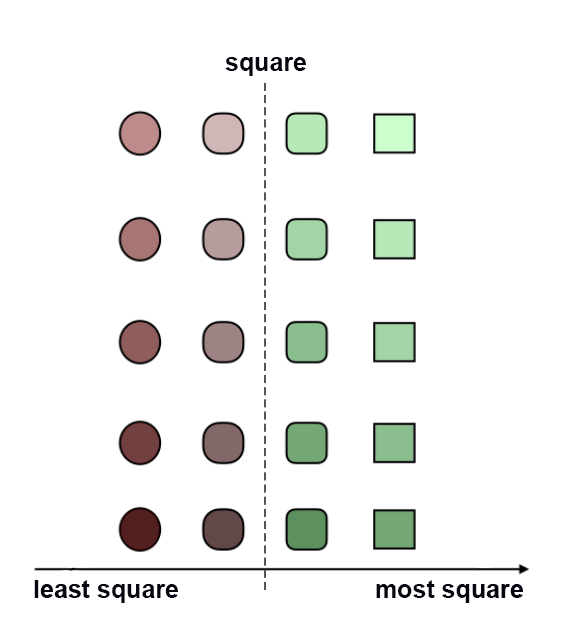
\includegraphics[width=250px]{images/Toyhyperplane1Direction.png}
	\centering
	\caption{An example of a hyper-plane in a toy domain of shapes. The hyper-plane for the word square is the dotted line. Green shapes are positive examples and red shapes are negative examples. \hmark{The arrow along the bottom of the figure indicates the corresponding direction. Those shapes far from  the hyper-plane on the right (positively classified) side of  the direction are more square than those in the opposite direction}}
\end{figure}

\hmark{These kind of} directions in document embedding models\hmark{, that go from documents that least represent a semantically meaningful word to those that most represent it,} can be useful in a wide variety of applications. \hmark{The most immediate example is being used as features in a simple interpretable classifier. In Figure \ref{ch1:introdectree}, an example of a decision tree that uses the semantic features obtained in this thesis limited to a depth of three is shown. This example is from a domain where text documents are movies, represented by a concatenation of movie reviews. The task is to classify the genre of the movie, and this tree classifies if a movie is a sports movie using semantic features derived from a vector space embedding.}

\begin{figure}[t]
	\label{ch1:introdectree}
	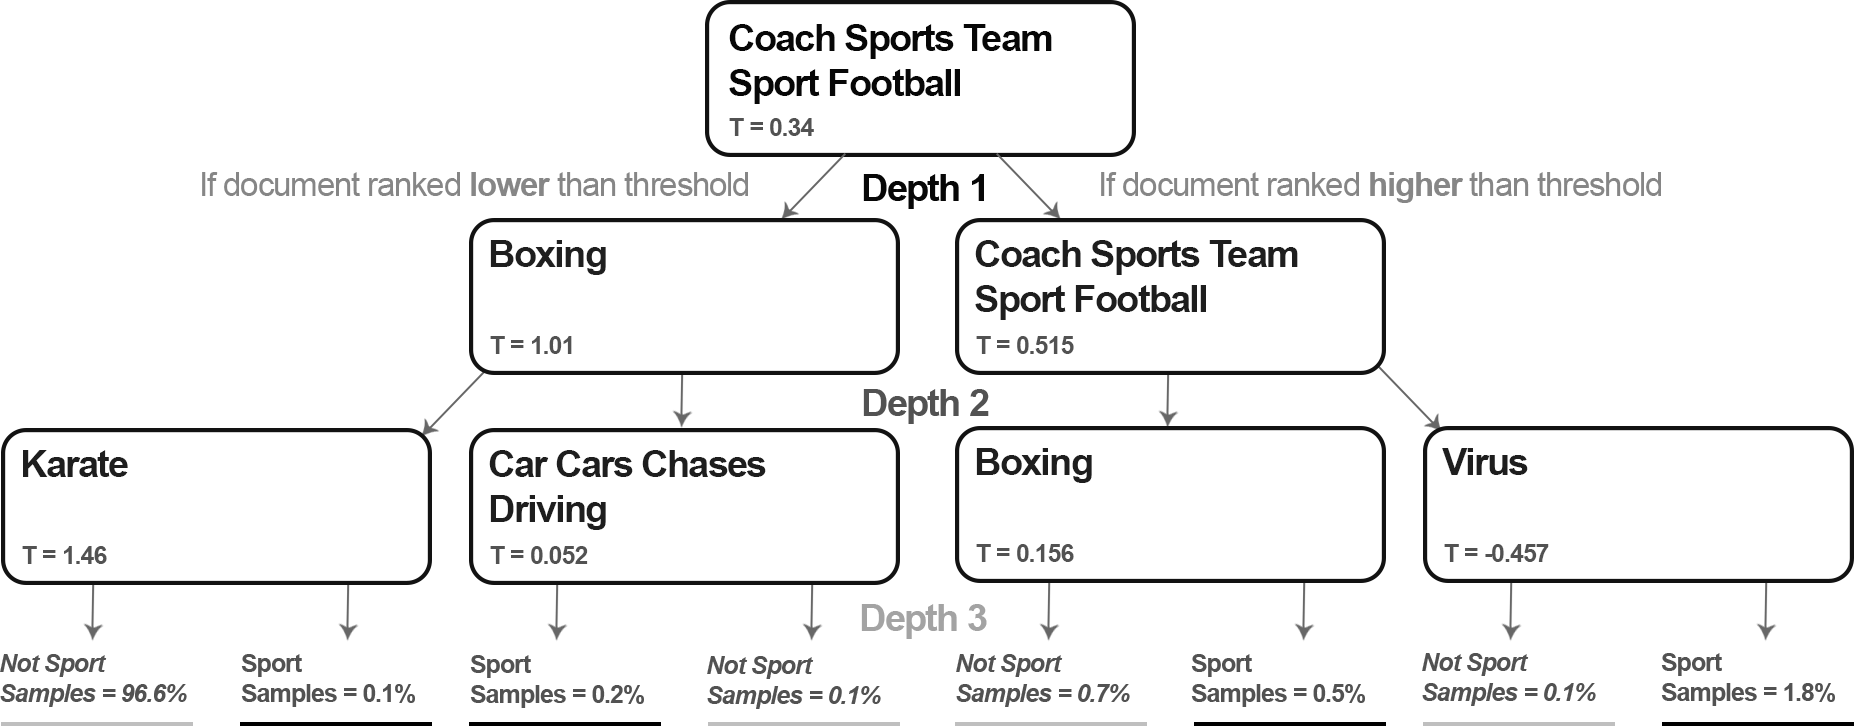
\includegraphics[width=450px]{images/decision_tree_ex.png}
	\centering
	\caption{An example of a Decision Tree classifying if a movie is in the "Sports" genre. Here,  decision tree nodes use features that capture properties of the domain. These properties are represented by keywords or clusters of keywords.  "Coach Sports Team Sport Football" is a cluster of keywords, that refers to the property in the domain of sports and sport, described using those words and related words like coaches and teams. This  property is extremely useful for classifying if the movie is in the "Sport" genre, and as such is the first node of the tree. Other nodes, like "Virus" apply to only a very small number of samples}
\end{figure}


 \hmark{Another  example} is  that they allow for a natural way to implement critique-based recommendation systems, where users can specify how their desired result should relate to a given set of suggestions \cite{Viappiani2006}. For instance, Vig et al \cite{Vig2014} propose a movie recommendation system in which the user can specify that they want to see suggestions for movies that are "similar to this one, but scarier". If the direction of being scary \hmark{is captured as a semantic feature}, such critiques can be addressed in a straightforward way. Similarly, in \cite{Kovashka} a system was developed that can find "shoes like these but shinier", based on a document embedding model that was derived from visual features. Semantic search systems can use such directions to interpret queries involving gradual and possibly ill-defined features, such as "\emph{popular} holiday destinations in Europe" \cite{Jameel}. While features such as popularity are typically not encoded in traditional knowledge bases, they can often be represented as document embedding model directions.% Directions can also be used in interpretable classifiers, for example, Derrac and Schockaert \cite{Derrac2015} learned rule based classifiers from ranks induced by the feature directions.

% NEEDS REWRITE
% How a decision tree would work with these semantic features is like this...
% Explanation of the labels and what they mean
% A one-depth decision tree could perform well with a key concept identified for example




% A low-depth decision tree is a prototypical example of a simple interpretable classifier. Performance in a low-depth decision tree relative to the full representation is used for evaluation, as this demonstrates that information in the original vector space has  been retained, and that the features are semantic, as they can sufficiently capture key domain tasks with a small number of features. 
 %good these semantic features are  is evaluated by how well  low-depth Decision Trees perform on key classification tasks in the domain when using these semantic features as input. %As well as demonstrating the use of these features in an interpretable classifier, it can be understood that if, e.g.\ a one-depth decision tree performs well on a key domain task then the representation is capturing a key feature in the domain, as a one-depth decision tree can only use a single semantic feature.  Similarly, in a tree limited to a depth of two, only a few features can be used, so to achieve good classification results, the features must capture particularly important meaning in the domain. An example of a low-depth  Decision Tree, classifying if a movie is a "Sports" movie, is shown below in Figure \ref{ch1:DecisionTree}. To give another example, when classifying if a movie belongs to the Horror genre, strong performance of a depth-2 decision tree suggests that the semantic features are used in the tree that are highly predictive (individually or jointly) of this class, e.g.\ features like "Scary" or "Bloody".



%Decision Trees have nodes that correspond to features, so if these features are simple and easy to understand then the tree is also interpretable \cite{Ustun2014}. 

%\hmark{The intention of this thesis is to post-process existing vector-space representations, disentangling the meaning they represent into semantic features. Relevant semantic features for classification can enable simple interpretable classifiers to perform well, without complexity that may be difficult to navigate without an expert user.  Low-depth decision trees are a prototypical example of such a simple interpretable classifier. 
% This chpater proceeds as follows...
 \hmark{Although the semantic features derived from vector space embeddings do have labels, the intent of this thesis is not to optimize these labels for interpretability. Rather, the intention of this thesis is to develop methods that can transform given vector space representation, such that components of the resulting vectors  correspond to semantically meaningful (i.e.\ predictive) properties from the considered domain. Such a representation is called "disentangled" - a representation composed of these properties is a disentangled representation.  }


  This chapter continues as follows: In Section \ref{ch1:hyp} the research hypothesis for the thesis is posed. This is followed by an introduction of three research questions in Section \ref{ch2:rq}, each corresponding to a chapter in the thesis. The contributions of each chapter are  then described in Section \ref{ch2:con}, and the structure of the thesis is laid out in Section \ref{ch1:ths}. 

%%%%%%%%% Disentanglement stuff
%There are a variety of existing approaches to obtain semantic features, historically  Principal Component Analysis has been used to obtain features of facial images \cite{OToole1993}, and more recently Bengio \cite{Bengio2012} identified a desirable property for unsupervised representation learning called "disentanglement". Disentanglement, to "disentangle" factors of the domain that account for variation in the examples, has been used in a variety of domains, in particular in by adjusting the learning methods of particular neural networks e.g.\ in a domain of handwritten digits images,  separate  features are obtained that represent the  "style" of the digit, and the  digit that was written \cite{Chen2016}. In the case of text domains,  a representation was  learned that  has  separate features for the sentiment of the text and the  content  of the text  \cite{John2019}, and in a medical text domain a representation was  learned with features corresponding to key medical aspects\cite{Banner}. } 


%\hmark{Although the intention of disentanglement is similar to that of this thesis, it is typically intrinsically linked to  a neural network structure, like a Generative Adversarial Network, and obtained by adjusting the learning method by e.g.\ requiring features to be independent from each other \cite{Banner}  \cite{Paige2016}. Other approaches to obtain semantic features, for example word vector representations, achieve sparse representations with semantic features by e.g.\ adapting matrix factorization to include sparsity constraints \cite{Murphy}. Our approach has its own focus in two main ways. The first is that this method  obtains semantic features from text documents, and the second is that this thesis focuses on  post-processing existing vector spaces. In particular, this is done by identifying  \textit{semantic relations} in the existing spatial representation and obtaining semantic features from them in an entirely unsupervised way. }





%One way to obtain a representation of the data that results in strong performance is feature engineering [cite], integrating encoded domain knowledge [cite], or using experts to validate the features [cite].  Manually hand-crafting or improving features takes time and knowledge that is not available for many domains, and so methods have been developed to learn features from data without the need of hand-labelling or encoding expert knowledge [cite].

% What are vector spaces? Why are they used? Why are they important and what are they a part of? What are their disadvantages?




%




% What is disentanglement? How does it relate to machine-learning feature Interpretability?  Why is it important?

 % and overlapping regions occur that correspond to properties of the domain (e.g.\ "tasty", "acidic", "bitter", "exotic"). Below, an example is shown of such a vector space.
 
%



%







%\hmark{This use of low-depth decision trees clarifies our aims. One aim is semantic features, which are validated through the classification of key domain tasks using a low-depth decision tree, and the second aim is for these semantic features to be useful for a simple interpretable classifier, which is validated by achieving strong performance without complexity. The idea of a disentangled representation of semantic features  is linked to the objective of interpretability.} 



%Other work which has taken advantage of directions in vector spaces has relied on word embeddings (See Section \ref{bg:WordVectors}). For instance,  \cite{gupta2015distributional} found that features of countries, such as their GDP, fertility rate or even level of CO$_2$ emissions, can be predicted from word embeddings using a linear regression model.   In \cite{kim2013deriving} directional vectors in word embeddings were found that correspond to adjectival scales (e.g.\ bad $<$ okay $<$ good $<$ excellent) while \cite{Rothe2016} found directions indicating lexical features such as the frequency of occurrence and polarity of words.

 %and potentially leading to better generalization, increasing the potential for transfer learning, and resulting in more efficient unsupervised learning  \cite{Banner}  \cite{Paige2016}.   





%Firstly, there are not many approaches that can induce disentangled representations in the domain of text, as 

%"Thus far in NLP, learned distributed represen-
%tations have, with few exceptions (Ruder et al., 2016; He et al., 2017; Zhang et al., 2017), been en- tangled: they indiscriminately encode all aspects of texts. Rather than representing text via a mono- lithic vector, we propose to estimate multiple em- beddings that capture complementary aspects of texts, drawing inspiration from the ML in vision community (Whitney, 2016; Veit et al., 2017a)" \cite{Banner}

%Benefits of disentanglement: Knowing if the model will generalize, transfer learning, more effiicent training when supervised objectivers are not aviavlalb,e  









%Methods that obtain interpretable representations include topic modelling with e.g.\ Latent Dirchlet Allocation (LDA), Negative Matrix Factorization (NMF), among others. 


% What does this thesis do to address that specific case?

% that by separating the key properties of the domain into features,
%The advantage of disentangled representations in this regard is that if the properties of disentangled representations are indeed distinct important concepts in the domain, then that is a first step towards a representation where each feature can be understood by humans. From that representation,  effective machine-learning models can be learned that can explain themselves using these features. However, 

%sHowever, these methods lack the flexibility and broad usage of vector spaces, which are applied in a variety of tasks and are a primary component of neural networks, a method that achieves state-of-the-art in many tasks using text data and in other domains.  

%This thesis offers a new approach for obtaining good disentangled representations, crucially being unsupervised, applied in the text domain, and used as a post-processing step on existing vector space representations. From these features, standard requirements like clustering, classification using simple classifiers, and understanding domains can be achieved, while using the information stored in a representation learned using a large volume of data from e.g.\ a complicated neural network architecture. 

\section{Hypothesis}\label{ch1:hyp} 

%Research hypothesis is the start-  don't give it all away - we dont know what we are doing
%(The previous work no clear rhyme or reason to what works)
%Use "disentangled" not "interpretable" because we are not concerned with labels
%In particular, claiming they are "interpretable" doesn't make sense 
%Provide a useful inductive bias to classifiers, across a range of domains and a range of different vector spaces
%High bias, less noise more robust beause it can only use those features
%Linear classifiers are robust because they can only find things that are linear
% - What is the best way to use linear models to  obtain a disentangled representation semantic features by using words and a linear model
%Question 2: Useful qualitative insights into the characteristics of the layers of neural network models
%Question 3: How can the quality of the features be improved by fine-tuning the vector space

%Vector spaces of text documents encode semantic relationships spatially, e.g.\ in a domain where documents are amazon product reviews, a vector space that is successful at sentiment analysis will be organized such that documents that are negative (i.e. a one-star review) about the product are distant from those that are positive (i.e. a five-star review), and there will be reviews inbetween (two, three or four star reviews). 

\hmark{Semantically meaningful features can be obtained from vector space representations of documents. These features are sufficiently predictive to be useful for simple interpretable classifiers, of which low-depth decision trees are a prototypical example, allowing for a performance that is close to the performance of an unbounded decision tree using the same features as input. Further,  these feature can be obtained from neural network hidden layers, and can provide valuable insights into  aspects of the domain that the neural network has learned. }



%Vector space models of text documents can be re-organized into interpretable feature representations. These interpretable feature representations are useful when used in simple interpretable classifiers of key domain tasks, as their features correspond to important properties in the domain. They are effective in multiple domains and can be derived from many types of vector-space. These interpretable feature representations can be made more accurate to domain knowledge and more interpretable with simple unsupervised procedures that ensure they more closely match a bag-of-words.

\section{Research Questions} \label{ch2:rq}

\textbf{Question 1:} \hmark{Can meaningful semantic features be characterised as directions across a wide range of vector space encodings and domains, and do these semantic features allow us to learn effective low-depth decision trees?}

\textbf{Question 2:} \hmark{Can semantic features be obtained from the hidden layers of neural networks, and to what extent can these features be used to  investigate  the characteristics of   different neural networks?}

\hmark{Question one and two focus on obtaining semantic features. However, this is not the intention of the final research question. Instead, this question looks at how to improve existing semantic features. In particular, by using a neural network to fine-tune the initial vector space embedding so that the directions contained within it are better suited for use as semantic features.}

\textbf{Question 3:} \hmark{Is it possible to obtain higher-quality semantic features in an unsupervised way by fine-tuning the initial vector space?}

\section{Contributions} \label{ch2:con}  

\hmark{In the work by Derrac and Schockaert  \cite{Derrac2015},  three domains were investigated  with all results  based on the same document embedding model. Then, these methods were evaluated with fixed hyper-parameters and a rule-based classifier.  In Chapter \ref{ch3} we propose a methodology for quantitatively validating the method and variants of the method by Derrac and Schockaert \cite{Derrac2015}, by using low-depth Decision Trees, limited to a depth of one, two or three. An extensive quantitative and qualitative evaluation is performed with the method and variants of the method, using data from five different domains, and vector space embeddings  derived from a variety of document embedding methods.  This is important to confirm the generality of the results from \cite{Derrac2015}.}  %\hmark{It is found that low-depth decision trees perform just as well as more complex decision trees in most cases, and indeed outperform complex decision trees in a few select cases.} 


In Chapter \ref{ch4}\hmark{,} the method \hmark{from} Chapter \ref{ch3} \hmark{ is used to obtain semantic representations from  the hidden layers of neural networks}, \hmark{in particular} feed-forward networks and auto-encoders. Specifically, the output of the activation values of the hidden layers  of the trained models are viewed as vector space representations,  and  disentangled feature representations are derived from them. Feed-forward networks are trained on supervised data to classify key domain tasks, and the disentangled feature representations derived from these feed-forward networks are quantitatively tested using depth-3 decision trees. The predictive performance of these decision trees is compared to the neural networks, and it is found that not much predictive performance is lost in most cases, and in one case, the disentangled feature representation obtained from the neural network when used as input to low-depth decision trees  out-performs the neural network it was learned from.  Further, characteristics of feed-forward networks are identified, in particular that they represent new semantic features that are more relevant to the class. \hmark{ However, the same experiment repeated for the stacked, meaning multi-layered, auto-encoder yielded a negative result.} \hmark{Furthermore, the properties in a stacked denoising auto-encoder are quantitatively and qualitatively investigated, and a method} is introduced to induce rules that describe relationships between semantic features from each layer, and the application of this method to  better explain how the neural network represents information is explored. This work was published in NeSy 16, the Eleventh International Workshop on Neural-Symbolic Learning and Reasoning.
%  Following this, a qualitative investigation is conducted of  auto-encoder features and it is found that the words used as features become increasingly frequent the deeper the layer of the auto-encoder they were derived from.} 





In Chapter \ref{ch5} we identify an issue with the use of the  centred objective used to build the vector space embedding. Specifically, although the vector spaces can be re-organized into meaningful directions, the similarity objective can sometimes be counterproductive. An example of this in a two-dimensional toy domain is shown in Figure \ref{ch1:toyExample}, where the similarity objective results in an outlier. Following this, a method is introduced to fine-tune the vector space, improving the directions in the vector space embedding at the expense of modelling similarity. First, Positive Pointwise Mutual Information (PPMI) scores for the words that label the interpretable features are obtained. Then, a target ranking for each feature is found by using isotonic regression to obtain values in between the PPMI scores and the rankings of the documents. This target ranking is used to train a single layer neural network with a non-linear activation function that attempts to match the rankings of documents to the target ranking. The intention is not to achieve 100\% accuracy, but instead to rearrange the rankings so that similarity based information is de-prioritized if it allows us to learn more meaningful directions. \hmark{Using these new properties as input to low-depth decision trees results in a performance increase for a variety of configurations and tasks, with some exceptions.} A qualitative investigation shows that the document rankings become more specific and meaningful for the features. This work was published in The SIGNLL Conference on Computational Natural Language Learning (CoNLL) 2018.

\begin{figure}
	\centering
	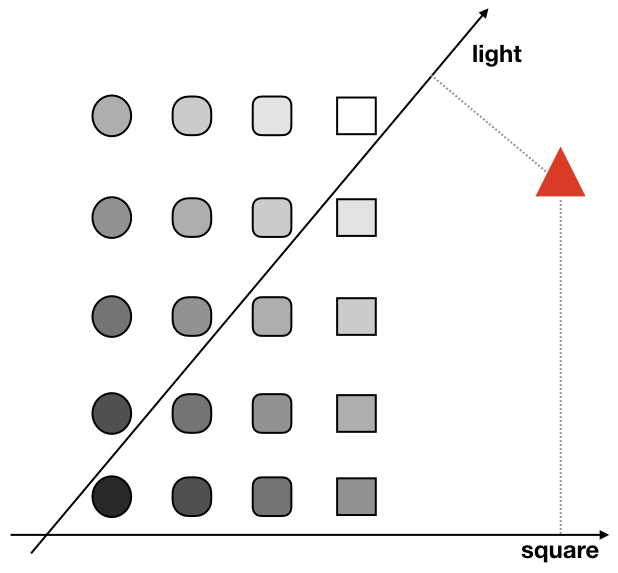
\includegraphics[width=180pt]{images/shapes}
	\caption{Toy example showing the effect of outliers in a two-dimensional embedding of geometric shapes}
	\label{ch1:toyExample}
\end{figure}

%In particular, we use this method of building a representation of entities as a way to convert a vector space into an interpretable representation, for use in an interpretable classifier. The reason that we chose this representation to expand on is because by representing each entity $e$ with a vector $v$ that corresponds to a ranking $r$, the meaning of each dimension is distinct, and we are able to find labels composed of clusters of words for these dimensions. Here, we make the distinction between a property and a word, a property is a natural property of the space that exists in terms of a ranking of entities, and words are the labels we use to describe this property.

%%% HYPOTHESIS


% Introduction to the internet, data, basic text representations
% Introduction to machine learning, benefits of data for machine learning, machine learning representations
% Problems with machine learning, interpretability, lack of interpretability in machine learningg
% We introduce a series of methods for transforming uninterpretable machine learning representations into interpretable ones
% Finding directions in vector spaces and using those to produce interpretable representations
% Fine-tuning these directions to get a better result
% Interpreting and investigating neural networks with these directions


%This brings up an essential point: When using a semantic space, are we taking advantage of relationships that are discriminative or incorrect? The danger of relying on these spaces and the models that use them has greatly affected their adoption in critical application areas like medicine, %Citation needed
%and has raised legal concerns about their application in e.g.\ determining if someone is suitable for a loan. 


\section{Thesis Structure} \label{ch1:ths}

\begin{itemize}
	\item \textbf{Chapter \ref{ch2}} gives an overview of methods for processing unstructured text data, standard machine-learning classifiers, and it provides a background \hmark{on other methods to discover semantic features and on related work in interpretability}.
	\item \textbf{Chapter \ref{ch2.5}} introduces and explains the datasets used in this thesis, as well as \hmark{explaining} the hyper-parameters  used for the machine-learning models in this thesis.
	\item \textbf{Chapter \ref{ch3}} provides a comprehensive quantitative and qualitative analysis of the method introduced by Derrac and Schockaert \cite{Derrac2015}, across a much broader group of domains, tasks, and vector space embedding methods. This section introduces the use of low-depth decision trees as a mechanism for evaluating the quality of the learned semantic features.  \hmark{Additionally, for the sake of completeness, variations of the method are introduced, with scoring functions that were previously not used, such as  NDCG, F1-score and accuracy. Standard k-means is used as an additional clustering algorithm that provides a reference point to the variation of k-means used in the original work. All variations, parameters, entity embedding methods and domains are comprehensively analysed and compared. }
	\item \textbf{Chapter \ref{ch4}} qualitatively investigates the use and application of the method in Chapter \ref{ch3} to neural networks, in particular feed-forward networks and auto-encoders. A rule-based classifier is used to connect properties between layers of an auto-encoder.
	\item \textbf{Chapter \ref{ch5}} introduces a  method to improve the interpretable feature representation by prioritizing these features over the similarity information that is captured in the vector space.
	\item \textbf{Chapter \ref{ch6}} provides conclusions on the contributions of this thesis and outlines a number of possible avenues for future work.
\end{itemize}


\section{Summary}

\hmark{Vector space representations of text documents are common in Natural Language Processing (NLP). However, their features are typically not interpretable.  There is an increasing need for suitable solutions to interpretability in NLP and machine-learning. A prototypical example of a simple interpretable classifier is a low-depth decision tree. A low-depth decision tree is effective when  semantic features are used as input. These features  correspond to properties of the domain that are suitable for the class, e.g.\ A property that represents the property of a movie being "Bloody" when classifying if a movie is a "Horror". This thesis studies methods for inducing such semantic features from a variety of vector space encodings of documents, including neural networks.}





%Shouldn't this be a summary of the chapter, rather than a summary of the thesis? If so, the story should rather be:

%* Vector space representations of documents are common in NLP. While they perform well, they are also difficult to interpret
%* Interpretability is an increasingly important challenge for NLP and ML, with small decision trees a prototypical example of an %interpretable classifier.
%* But such classifiers can only be effective if they have access to the right semantic features.
%* The aim of your thesis is to study methods for inducing such features from a variety of vector space encodings of documents.



% Our work is...

%\section{Relationships}

%Vector spaces are representations that reduce the dimensionality of sparse representations like bag-of-words into dense spaces where semantic relationships e.g.\ two movies being similar to one another, are represented spatially. However, upon reducing this dimensionality the features are no longer interpretable.  One way to interpret what these vector spaces mean follows Conceptual Spaces \ref{????}, where entities in the domain e.g.\ movies in a domain of movie reviews are represented as points, and properties in the domain are represented as convex regions. The work in Chapter \ref{ch3} details a process where the vector space is transformed so that these properties are used as features, creating an interpretable but dense representation. The introduction goes into further detail about these properties.
% Conceptual spaces

% properties

% using properties as features

%\section{Contributions}\label{ch1:contributions}

% chapter 3 does this
%etc

%\section{Representations}




%\section{Motivation}
%What is text? How is it motivating?

%What are the desiradata of a good representation?
% Unsupervised


%One task of Natural Language Processing is to obtain this semantic understanding from text by obtaining a machine-readable representation that contains domain knowledge. A basic approach to obtain a representation of this text is to represent entities (e.g.\ reviews, text-posts) by the frequency of their words, see \ref{Bag-of-words-example}.

%\begin{figure}[t]
%	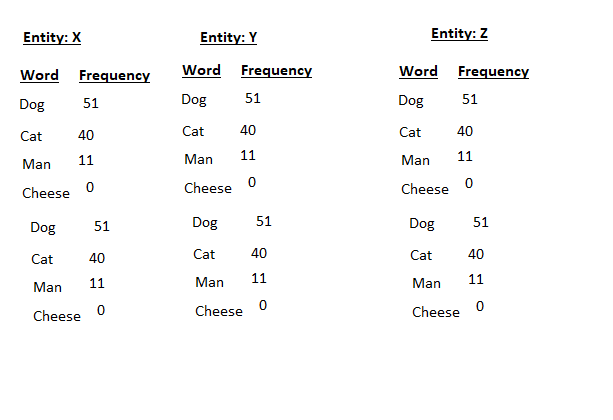
\includegraphics[width=\textwidth]{images/bowbowbow.png}
%	\centering
%	\caption{Bag-of-words  }\label{Bag-of-words-example}
%\end{figure}


 %Below, we show a review with its associated properties labelled.

%\begin{figure}[t]
%	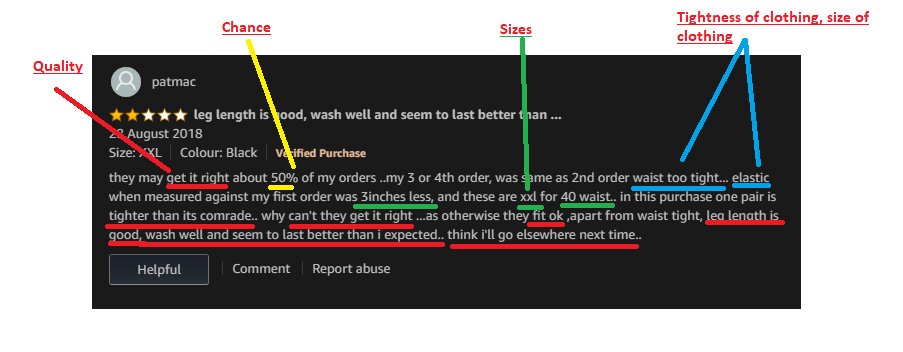
\includegraphics[width=\textwidth]{images/leg_length.png}
%	\centering
%	\caption{Example properties  }\label{IntroDecisionTree}
%\end{figure}

%\subsection{Machine Learning}
% what is machine learning? why do i care?


% Granular
%We can understand these properties to have a degree to which they apply, for example the size of the clothing might be "XXL", "XL", "L", "M" or "S", or the quality may be "Very good", "Good", "Ok", "Bad" or "Very bad". For the former, we may rely on the metadata available from the site itself, but for the latter the way to obtain this information is less clear. Although we may infer that the rating has some indication of these properties, it does not describe the properties or the degree to which the review refers to them. %This kind of information is valuable for making sense of the world of unstructured text, and has broad applications, e.g.\ The most immediate example is perhaps that they allow for a natural way to implement critique-based recommendation systems, where users can specify how their desired result should relate to a given set of suggestions \cite{viappiani2006preference}. For instance, \cite{Vig:2012:TGE:2362394.2362395} propose a movie recommendation system in which the user can specify that they want to see suggestions for movies that are "similar to this one, but scarier". If the property of being scary is adequately modelled as a direction in a semantic space of movies, such critiques can be addressed in a straightforward way. Similarly, in \cite{kovashka2012whittlesearch} a system was developed that can find "shoes like these but shinier", based on a semantic space representation that was derived from visual features. Semantic search systems can use such directions to interpret queries involving gradual and possibly ill-defined features, such as "\emph{popular} holiday destinations in Europe" \cite{DBLP:conf/sigir/JameelBS17}. While features such as popularity are typically not encoded in traditional knowledge bases, they can often be represented as semantic space directions.  %Copied from CONLL

%\subsection{Directions}\label{intro:directions}


%However, manually labelling these properties and the degrees to which entities (e.g.\ reviews, text-posts) have them is extremely time-consuming. 

%A potentially ideal system would be as follows: We collect large amounts of unstructured text data, separated into domains, and obtain the properties of each domain from this data, and rank entities on the degree to which they have these properties. In this way, properties would be understood on a scale built from the domain directly, so that each domain has its own meanings for words according to their own idiosyncrasies. As the process does not require any manual labelling the quality of these properties could be improved simply by obtaining more data. Further, as we are learning from unstructured data, not only would this allow us to understand the data in terms of what we know, but it would also introduce us to new ideas that we may not have previously understood. This kind of representation also has value in application to Machine Learning tasks. If we can separate the semantics of the space linearly into properties, we are able to learn simple linear classifiers that perform well. 

%Simple linear classifiers built from a representation composed of rankings on properties have an additional benefit of being more understandable.


% Natural clustering
% Semantically distinct
% Interpretable
% Curse of dimensionality
% Generalizability ("shared factors across many tasks" \cite{Bengio2012})

%What is machine learning? What are its advantages? How is it motivating?

%What are the problems with machine learning? How is it motivating?


%What is domain-specific? What is domain knowledge? %On the web there is a large volume of raw text data, e.g.\ Reviews of products, movies, anime, books, music, social posts by individuals, self-descriptive text about a website or product, and so on. These can be categorized into domains; each domain has its own quirks, knowledge, and method of being brought about. Although a movie review may sound similar to a book review, they typically differ hugely in the distribution of words used.

%

%\section{Interpretability}\label{ch1:interpret}

%What is interpretability? How is the value of interpretability measured in the real world?

%How can we meet the needs of the real world?  Is it transparancy, the system having easy to understnad components, etc... what  are the different views on what an interpretabile system is?

%What specific interpretability task are we trying to solve? How do we define interpretability? Why is it valuable, where is it used? What was the hypothesis/research question?
%%What are distributional models?
%Most successful approaches in recent times, like vector-spaces, word-vectors, and others, rely on the distributional model of semantics. This model relies on encoding unstructured text e.g.\ of a movie review, as a vector, where each dimension corresponds to how frequent each word is, we are able to calculate how similar the entities are, e.g.\ we know that if two movies have a similar distribution of words in their reviews, like frequent use of the word 'scary', or 'horror', then they would have a higher similarity value. These models, also known as 'semantic spaces' encode this similarity information spatially.

%Semantic relationships can be obtained from semantic spaces. 

%applications/need for good interpretability:

%What is a conceptual space? What are entities?  What are properties? What is commonsense reasoning?
%properties of an interpretable classifier:
%\begin{itemize}
%	\item Complexity: 'the magic number is seven plus or minus two' \cite{Saaty2003} also has many positive effects for its users, like lower response times \cite{Narayanan2018, Huysmans2011}, better question answering and confidence for logical problem questions \cite{Huysmans2011} and higher satisfaction \cite{Narayanan2018}.
%	\item Transparancy: 
%	\item Explainability: 
%	\item Generalizability:
%\end{itemize}


%X%X%What is a symbolic approach?  %One approach to making sense of these domains is to produce rules from expert knowledge. An expert in movies would tell you that if the review talks about it being a "cannibal horror film", we can understand that it is likely a scary movie and is related to the original 'Cannibal Holocaust' movie. Encoding this kind of knowledge is difficult, time-consuming, and hard to automate reliably.

%Properties, entities, the benefits and application of a representation formed of these

%Basic introduction to directions, explanation of the utility and application of our approach
%\section{Thesis Overview / Contributions}

%What were our objectives starting out? 
%What are our intentions with how the work in the thesis will be used?
%What are our contributions?
%%What are our aims for this chapter? What do we overall want to do? (Already kind-of said in Chapter 1, but worth repeating I guess in some form)
%In \ref{Chapter3}, we introduce a pipeline that starts with unstructured text, and ends with an interpretable representation of entities represented by properties labelled by clusters of words. Further, we demonstrate the applicability of these representations in a simple Decision Tree that uses just a few of these properties to classify entities. In Figure \ref{ExamplesWithTree}, we show some example movie entities, their associated properties, and a Decision Tree classifying whether or not they are a Horror movie. 


\chapter{Background}
% What text representations actually are
% Why text representations are useful, what they are used for, how do they relate to our work, how do they relate to interpretability
% Classification, what classification is, example with Decision Tree
% What semantic spaces actually are
% Examples of classification with SVM's 
% What interpretable representations actually are, desiradata/features of interpretable representations
% Examples with Decision trees, examples of classifiers that produce an interpretable result automatically


% Main ideas im setting up


% Vector spaces contain semantic relationships

% Vector spaces are not interpretable

% Interpretable means that the dimensions are meaningful

% Neural networks contain vector spaces

% Simple interpretable classifiers are valid


% Introduction
% What the general process is for learning and solving problems

% Text data
% The problems of text data. Why it's interesting. How to solve and contribute to solving those problems. What kind of semantic information we might want from text data. How to get that better

% Text representations
% Bag-of-words is a standard representation. It contains this kind of information. This kind of information is surprisingly suitable for solving tasks. The problem is its sparse and doesn't describe relationships.
% Vector spaces make them dense and describe relationships

% Neural networks
% Neural networks are a general thing that can do supervised or unsupervised tasks including making representations, they contain and create vector spaces
% Word vectors are big in NLP and use neural networks to integrate context
% Disentangled representations and conceptual spaces

% Interpretability
% The biggest problem with vector spaces is that they arent interpretable.

% General conclusion
% There are a lot of different ways to represent nlp information, and nlp information is important to represent well and solve well. But we want it to be interpretable as well. So how can we obtain a method that can use all of the information stored in these vector spaces, including complex ones created by neural networks, and create an unsupervised representation method to get interpretable representations? thats the next chapter


% What are text representations composed of? Why do text representations matter? Why does the other stuff matter?  How will it be used in this thesis? Why should I read this chapter?
%Labels, features, models, representations, regression, classification

\section{Introduction}

This Chapter begins by explaining the general process required to solving tasks with machine-learning starting from raw text data. The steps of this process are expanded on in the later sections.


Similar to how it would not be possible for a human to solve a problem without a good understanding of the subject area, the first step of solving a problem with  machine-learning  is to obtain a suitable  representation of the data. If this "understanding" or representation is not good, then no matter what steps are taken to try and solve the problem then they will not yield good results. In this thesis a representation must be obtained from raw text data that is effective for the task of document classification. Document classification is the task of distinguishing between entities in a domain, where entities are e.g. movies in a domain of movie reviews, people in a domain of twitter posts, or reviews in a domain of product reviews. 

As the task is to separate entities, after data collection the first step of solving the task is to separate the corpus of text into a document for each entity. Then, the text is pre-processed so that noise is removed, "noise" in this thesis refers to information in the text that is not useful when solving the domains document classification tasks. For example, metadata like the e-mail of a movie reviewer in movie review text, or unnessecary punctuation and grammar. It's important to remove this information at this stage as raw text data is easy to manipulate and the the result of any modifications can be clearly seen. If we tried to remove this kind-of information after obtaining a representation, it would be a much more complex process.

One popular and simple representation is the bag-of-words. The bag-of-words  represents an entity as a vector where each element corresponds to a unique word in the corpus. The values of these elements are usually some statistic related to the words importance in the document e.g. word frequency where if a word occurs five times in a document the value is five. One disadvantage of this representation is that it doesn't retain the context of words, another is that it is sparse, as each vector has an element for every word in the corpus and only some of them will have a frequency above zero. This means that the to store it and process it in memory efficiently, specialized data structures and machine-learning techniques must be used. However, it has the advantage of being easy to understand for humans as each element of the vector representation for each entity corresponds to a word. 

Ideally the number of dimensions would be reduced while retaining the information. One method of doing this would be hand-crafted feature selection, where words which are identified by experts as not meaningful are not included as an element. However, if it is done manually it would take a large amount of time and require expert knowledge, and  if this is automated a lot useful information can be lost to make the size of the data manageable. An alternative approach is to use the vector similarity between entities, e.g. the similarity between their frequency BOW vectors, to produce a low-dimensional vector space, where entities are encoded  such that their semantic similarity matches their spatial similarity.  In this space, the vectors that correspond to entities are just co-ordinates in a e.g. 2000 dimensional vector space. However, this results in vectors whose elements are no longer interpretable in the sense the bag-of-words is, instead information is stored as similarity relationships between entities in the vector space.



%For humans, our understanding of how things behave and what they are is a representation of reality,   produced from our experience with those things in the real world. Each person is constantly adjusting to some degree their representation of what different things are, and this construction and transformation of our personal representations is what we call learning. 

% Machines are computational and can process large amounts of information, but it must be in a suitable representation for them to use it.  For tasks in the domain, e.g. categorizing Amazon product reviews into positive sentiment or negative sentiment, it is usually required that the representation encodes fundamental domain knowledge. Put in terms of human intelligence, it is akin to how we must have some fundamental representation of the domain before we can appropriately act in it.

%In this thesis the data used is raw text, so a scalable computational representation of the meaning of text data is required.  There are a variety of methods to achieve representations of raw text data, and each one leaves out some information from the domain and prioritizes other parts. This makes each suited to solving a different problem. For example, the bag-of-words representation is called as such because word-context is ignored, but on a task of sentiment analysis word context is important, e.g. a review for a movie that contains the sentence "This was so good I want to rip my eyes out." although sarcastic, would still count as a compliment. To achieve better results on this task, it would be better to instead use a representation that can represent context somehow. In section \ref{ch2:representations} we cover how to obtain different kinds of representations and explain how they work.

%Determining  sentiment of e.g. an Amazon product review is one of many domain tasks that machine-learning can solve. This is specifically the task of categorization or "classification" that naturally occurs in many domains. For both humans and machines, the essential question when making these decisions is if the representation we have of the entities in the domain is accurate to the reality, i.e. if it represents Amazon product views well. As with the methods, there are many different ways to classify using machine-learning given a representation. However, there is no way a machine-learning classifier can perform well on a task without a good representation. Different classifiers that are used in this thesis are covered in section \ref{ch2:classifiers}.

%Growing up learning a language, people learn the complexities of that language intuitively and can recognize if something is wrong without necessarily being able to verbalize why. This is the problem of a representation that is difficult to express, and in-turn difficult to understand. In a similar way, representations for machines that can e.g. capture the context of words precisely can be difficult to understand for humans, as it is difficult to encode this complex information in a simple way. This is the problem of interpretability, taking representations and classifiers that are only intelligible to machines and making them understandable for humans as well. There are a variety of ways that more complex information can be represented interpretably, and this is covered in Section \ref{ch2:interpretability}. 






%There are a variety of different text representations, but the most common is the bag-of-words. A bag-of-words ignores word-context, instead using the frequency of terms in a document as its text representation. This representation is a matrix, where each column is a word in the vocabulary of the domain and each row is a document. 


%\subsection{Classification Problems}





%One example of an unsupervised machine-learning task is to transform data into a representation that can be learned from by the 



%\subsection{Interpretablility}

%Simple rules are a good basis for an interpretable classifier. However, this is only possible when the features (e.g. the word frequencies in a bag-of-words) are clearly defined. This forms the basis of what an interpretable representation is viewed as in this thesis. If the features correspond to some meaningful property in the domain, e.g. "good" or "thrilling", then that is treated as an interpretable representation. In this sense, a bag-of-words is an interpretable representation, despite the approach in this thesis being different from the methods a bag-of-words employs.


%\subsection{Vector Spaces}




%\subsection{Conclusion}

As mentioned in Section \ref{ch1:contributions} the main focus of this thesis is in transforming vector spaces into interpretable representations while retaining their information. This Chapter introduces the process of obtaining a representation from text data and using it to solve machine-learning problems, as well as giving a general introduction to related work. To outline the process, first as covered in Section \ref{ch2:data} the data is preprocessed so that unnessecary information is removed. Then some basic representations are obtained in Section \ref{bg:BOW} and this is followed up by more complex vector space representations \ref{ch2:vectorspaces}. To complete the process, Section \ref{ch2:classifiers} covers different machine-learning methods to solve problems using these representations. Finally, interpretable representations and classifiers are covered in Section \ref{ch2:interpetable} to give context in the literature for the work in the next three Chapters. 

%With the rise of services on the web that enable large-scale user-generation of text data,, the internet has become largely populated by text posts that are related to some specific, niche topic within a domain. For example, a review on Amazon for a product is specially tailored text for that product within the domain of Amazon reviews. Taken from a closer lens, we could even argue that each review-type has its own domain, e.g. Product reviews, Food reviews, Movie reviews. However, the text posts themselves are largely unstructured semantically. 

%Text data. Why text data? What useful applications does text data have? 

%The availability of text data has expanded as technology, in particular the web,  has taken a larger part of our day-to-day lives. The availability and volume of this text data has driven research into how to use it, solving problems like automatic language translation, predicted terms, or even detecting if a patient acquired an infection in a hospital from their recorded text data \cite{Ehrentraut2018}. The first question that needs to be answered is, 

%What is this section about? Why is it here? What will they get out of the end of this section? 

%In this Chapter, the fundamentals are covered that are required to understand how to go from text data to machine learning models that are useful in our day-to-day lives. The future Chapters introduce a new question following the previous paragraph, how can we make a representation that is intelligible to both humans and machines, and how can it be applied? In particular, Chapter 4 conducts a deep experimentation into simple interpretable models, Chapter 5 uses these models to gain insight into what other models have learned, and Chapter 6 refines them so that they perform better and are easier to understandw. 

%How do machines understand text data? How do machines use text data? 

%In the case of this work, we look at text split into documents, where e.g. in a collection of imdb movie reviews, each movie would be a document composed of all of its reviews. Exactly what composes a document depends on the dataset, but it is generally longer than a sentence and is an object in the domain, e.g. a news article in a domain of news websites

%Where does the background go from here? What do the remaining sections cover?

%This thesis is about learning interpretable features (See the discussion in Section \ref{ch1:interpret}). In this case, this means that each feature is labelled with words so that humans can understand what that feature means, e.g. in a domain where each document is a movie review, a bag-of-words is interpretable as it has the label "Scary" for a feature and its frequency value. However, this is only useful if we desired to classify

%This Chapter continues as follows: First we go-over the bag-of-words and improvements for it, then we move on to how to obtain representations that model more complex relationships between documents using a variety of methods. From there, we explain a few different types of classifiers and finally give more specific context for the work in the thesis, describing interpretable representations and other related work.



%These tasks can range from Document Classification where documents are organized into categories e.g. separating news articles into "World News" and "UK News" based on their text, to Sentiment Analysis where if a text document like a movie review is classified as positive or negative. Each of these tasks requires a different representation to be most effective, for example ideally when learning a Sentiment Analysis task the representation would model sarcasm and context e.g. representing that "Now, this wasn't bad" doesn't carry the same meaning as "Now, wasn't this bad". 


%Text documents, pre-processing


%Bag-of-words

%Vector spaces

%Word-vectors

%Linear SVM's

%Decision Trees

%Isotonic Regression

%Topic Models

%Clustering

%Interpretable representations



%Accuracy and F1

\section{Text Data}

This thesis is focused on producing interpretable representations from text data, and solving specific problems in text domains. In this section, the basics of what the text data is, terminology associated with it and how it is preprocessed is described.

\subsection{Text Domains}

"Text domain" refers to a subject area that is unique in its vocabulary and structure. One example is the newsgroups domain (See Section \ref{data:datasets}), which is composed of online news discussion groups from 1995. In this domain, there are subject areas, topics and posts. Each subject area has topics that users create, and each topic has posts that users respond with. Within each of these subject areas, specific jargon and a unique structure specific to that subject area and the overall domain has developed. Below an example post is provided from the newsgroups domain that contains unique jargon like "NOEMS", "EMM386" and a unique structure e.g. signing the post with the persons name and a personal tagline for contacting them.


\begin{quote}
Has anyone else experienced problems with windows hanging
after the installation of DOS 6?  I have narrowed the
problem down to EMM386.

If if remove (or disable) EMM386, windows is ok.  If EMM386
is active, with NOEMS, windows hangs.  If I use AUTO with
EMM386, the system hangs on bootup.

Dave.


-- 

-------------------------------------------------------------------

David Clarke   ...the well is deep...wish me well...

ac151@Freenet.carleton.ca  David\_Clarke@mtsa.ubc.ca  clarkec@sfu.ca
\end{quote}

These particularities to the domain are what makes the distinction between domain-specific text data to general text data. A machine-learning model will develop a representation of how to solve the task dependent on this data. If the model is given general text data examples to learn from, then it will miss out on domain-specific quirks that can help it solve the task e.g. when learning to identify if a newsgroups post belongs to the subject of windows, if the general examples do not use jargon like "AUTO" and "EMM386" then this important information will not be used. However, if the examples given are over-specialized then the model may place excess importance on domain-specific quirks that are not actually meaningful, e.g. if in the training examples of posts about windows most users signed off their text-posts with an email that includes ".ca", meaning they are from canada, then the model may identify all posts that include ".ca" emails as about windows despite this simply being a strange quirk in the data.

Although language is universal, the individualities of text domains make solving problems efficiently within those domains often depends on a domain-specific machine-learning pipeline where both the representation and the machine learning model that will solve the problem are catered towards that domain. For example, twitter posts are significantly shorter than newsgroups posts, and rely more on modern expressions of ideas e.g. using a joke format that others on the platform have used. Being able to make-use of these domain-specific insights somehow in the process is extremely important. 

In this thesis we aim to introduce methods that can be used to a variety of domains and be used with a variety of machine-learning models, without labour from domain experts. In particular, we look at solving domain-specific tasks without catering the representation or the model to the domain using expert knowledge. With this in mind, the following sections will be focused on a more general pipeline that does not delve into domain-specific techniques.


%One goal of machine-learning is to predict if a piece of text will be shared or liked by users. In this case, it is clear that in-order to determine if a movie review will be liked or shared, it is difficult to determine if that will be the case when using the same logic that you would for a facebook post. Facebook posts that trend or are well-liked are typically brief, easily consumed and focused on humour. Meanwhile, movie reviews that trend are due to cutting and intelligent analysis of a movie in a relatable way. 


 %text data available from a domain is unique to that domain in many ways, for example on the social media site Facebook text data can be formatted into posts and comments, and is posted by users. Although a movie review by a critic could on the surface have the same structure - a post with comments below, the rules governing what is contained in the post are clearly not the same. 



%The main point here is not that these domains are completely different, but rather that there are meaningful differences between between text from the domain and text outside of it, and although there are different rules for each domain there are still common trends between them. Typically in machine-learning the methods that perform the best use some-kind of large-scale data that is not directly related to the domain as well as a lesser amount of domain data.


% Text from different domains is formatted differently, e.g. posts and comments
% Corpus are usually split into documents because of its associated tasks, give examples?
% Text from different domains differ in language
% Tasks in different domains are different
% Text from different domains perform better using different representations and classifiers
% There are similarities between domains that is taken advantage of e.g. using word-vectors
















%EXAMpLES SOURCE ETC




\subsection{Pre-processing Text Data}\label{ch2:data}


% Corpus are split into documents

Text documents in a domain usually reflect task that needs to be solved. In a domain-specific classification task, e.g. identifying the genre of a movie in a domain of movie reviews from its review text, the subject of the task are entities in the domain, in this case movies. A natural way to arrange the data is to create a document for each entity that contains all of its related data. For example, putting all the reviews for one movie in the same document. This is what is meant by a document-based task, where the corpus is arranged into documents that correspond to entities in the domain. In this thesis, we focus on these document-based domain specific tasks. 

% We just use the raw text data without modifying it.

%There are a variety of ways to add additional structure to raw text, one-such way is to label parts-of-speech (known as POS tagging) like nouns, adjectives, or other grammatical constructs. This can be done automatically with reasonable accuracy, however there are not many datasets with this kind-of structured information available, and it is difficult to achieve reliable results without experts annotating the data, which is costly and time-consuming. This thesis focuses on how to use raw text without adding additional structure or information. Using raw text without additional structure enables the method will have broad applicability and allows easy comparison with other work.




% Building a vocabulary
% What parts of text data do we want to keep?, % What is noisy data?
% There are many ways to preprocess raw text data using expert knowledge, but we focus on an unsupervised and machine-learning approach
% Standard rules to reduce noise

To obtain a good representation of a corpus, the text data must  be processed so that it contains as little noise as possible. What exactly noisy data is depends on the representation and the task, but for this thesis it can be seen as parts of the text data that are not meaningful when distinguishing between types of entities in the domain. Noisy text data can have a knock-on effect on the representations that are built from it, resulting in a much worse representation. If the email of a movie reviewer was retained in the review text, that will not be useful information for a task related to the movie. Additionally, you could also see  a word starting with an uppercase or lowercase as noise, as it is not information that will benefit the representation. %that if retained in the representation would harm it more than help it. Another example of noise that you would ideally like to remove is metadata,



% noise versus not noise - what does it mean?

Being able to automatically remove this noise is an essential step of building a representation and solving machine-learning problems.  The first stage of obtaining a bag-of-words is building a vocabulary $W_w$, composed of unique words $w \in W$ from the corpus. In this vocabulary, it is important that words which have the same meaning are not treated as different words e.g. if the word "Dog" was considered to be different to the word "dog." then the vocabulary would be too noisy. There are standard methods for removing noise in a dataset. We describe them in the following bullet-points: %In Table !!! we show some examples of noise in a domain.  %examles of noies!!!!

\begin{itemize}
	\item  Convert all text to lower-case, e.g. "The man and The Dog" converted to "the man and the dog"
	\item  Remove all punctuation including excess white-space, e.g. "the man, and the dog..." converted to "the man and the dog"
	\item Using a predefined list of "stop-words", listed in full in Table \ref{ch2:stopwords}, remove words that are not useful, e.g. "the man and the dog" converted to "man dog"
	\item Remove infrequent words, e.g. "man dog, dgo, dog man" converted to "man dog, dog man".
	\item Domain-specific pre-processing to remove metadata, e.g. removing emails from the end of movie reviews.
\end{itemize}






%When using a bag-of-words as a representation in a classification task, that threshold is usually set higher, as it is more important to remove noise that would not naturally be removed when using the bag-of-words to create another representation. 

%One way to remove noisy words is to apply a filter where words that are not frequent enough are removed. %Typically when creating a representation the threshold $T$ for this filter is low, e.g. two or one, so that only truly noisy words are removed. 

%%%%%%%%%%%%% Convert to a bullet point list with better organization

%However, if grammar and punctuation is removed then we can simply count that there are two occurrences of the word dog, resulting in a more robust way to count words. Some words are too common to be meaningful, to remove these words a list of "stop-words" is created - words like "the" and "and" resulting in a sentence that only contains meaningful words, e.g. "man dog dog man dgo". Finally, terms that do not occur more than a set threshold $T$ are usually pruned, with the lowest threshold being one. This is because terms which do not occur often are likely noise,   for example leaving us with a final representation of "man dog dog man", removing all remaining noise. 

%Despite removing some structure and making it less readable  at-scale this pre-processed sentence results in a better representation of the meaning of the text for machines. 

In this work and the representations used in this work, the  rules above are applied to the corpus beforehand. The methods are standardized so there should not be many interesting differences in the work, and it will also still be replicable. In terms of removing words that were not frequent enough, words that did not occur more than once are removed.  Although these rules are not universal, they are a good basis for computational methods of representing text data that do not rely on word-context and grammar. In the next section, we cover some  methods for text representation and explain their basic utilities.  %EXAMLES

\section{Text Representations}\label{ch2:representations}



% What is a text representation? Why is it usefl? What is a representation?

Humans can have an intuitive understanding of the semantics that are present in unstructured text, but machines do not.  Text documents like news articles, product reviews or social media posts cannot be classified without first being represented computationally.  Representations $r$ are composed of features $r = (x_1, x_2, ..., x_n)$, where ideally each feature $x$  is meaningful in the domain. For example, meaningful features when determining the  value of a house would be the amount of bedrooms $x_1$, and the amount of toilets $x_2$. An example vector from these examples would be $[5,2]$ for a house with 6 bedrooms and 3 toilets.


In the next Chapter of the thesis, as well as in section \ref{ch2:interpretability} how to make a representation that both humans and machines can understand is discussed. However,  this section  focuses on representations that are useful to machines when used for machine-learning, rather than being interpretable. In particular this section covers preprocessing data \ref{ch2:data}, sparse bag-of-words representations \ref{ch2:BOW} and obtaining vector spaces \ref{ch2:vectorspaces}.




%rom here, we can assume that 



%This thesis deals with text-document representations. Text documents are unstructured raw text data that have been separated according to their domain, e.g. Amazon product reviews separated such that each product is represented by all of its reviews, or news articles separated such that one document contains the data for one news article. One way to gain insight into this data is to count the frequencies of the words in each document. If a word is high-frequency for a document, then that word will likely be important to understand the meaning of that document. 

%Text data, for example forum posts, amazon product reviews, or news articles have become readily available as the digital infrastructure that supports our lives has grown. This data largely is unstructured, and cannot be readily processed by Artificial Intelligence tools without being reformatted. For example, if the text is separated into documents e.g. the raw text for one news article is put into a separate document from another.

%Need to write about the concept of salient features of a domain here.
\subsection{Bag-Of-Words}\label{bg:BOW}

The bag-of-words is a simple representation that can scale to an extreme amount of data. Although when looking to achieve state-of-the-art results representations that are more complex or tailored to the domain are used, with enough examples even a basic representation can have enough information to clearly distinguish between types of entities in a domain for a task. 

The bag-of-words (BOW)  ignores word context, instead taking the words that occur in each document and assigning a value to them in a matrix, e.g. where each word in a document is assigned a value for  its frequency in that document. For example, a short document of text like "there was a dog, and a man, and the man, and the dog" would be translated into word frequencies "there: 1, was: 1, a: 2, and: 3, the: 2, man: 2, dog: 2". This representation is simple, and ignores word context, grammar and punctuation but is highly effective when using machines to solve problems using a large amount of unstructured text documents. The bag-of-words is an important part of the work of this thesis, serving as the foundation of more complex and interpretable representations. 

As mentioned in the previous section, unnessecary parts of the data that are not  meaningful for the task should be removed. The bag-of-words is a representation that comes with the following assumption: the context of words is an unnessecary part of the data to perform well on the task. How correct this assumption is depends on the task, but despite this view being overly-simplistic the application and use of the bag-of-words (BOW) is broad. There are multiple ways to represent words in the BOW format, but the most common is by the frequency of the words in a document.

The natural structure for this kind of representation is that of a matrix, where rows are documents and columns are words in the domain as defined by their vocabulary. Specifically,  text documents in a domain $d \in D$ have an associated vocabulary of unique words across all documents $w \in W$. The bag-of-words $B_D$ is a matrix where each document is a row, and each column is a word, where the value of each word for a document is the word's frequency in that document $d = ({wf}_1, {wf}_2, ..., {wf}_n)$ where ${wf}(d)$ is equal to the frequency of a word in a document and $n$ is equal to the number of unique words  in the vocabulary for all documents $w \in W$. In terms of the general structure given above, our representation $r$  is the bag-of-words, and the features $r = (x_1, x_2, ..., x_n)$ are the word frequencies.

%Given these vectors we can determine the similarity between two documents or two words by the similarity between their frequency vectors or document vectors. %!!!!!!!!!EXamles???

\subsubsection{Term Frequency Inverse Document Frequency (TF-IDF)}

There are two main problems of using frequency is that words which are frequent in the domain are given a higher value than words which are used frequently only in a single document. First, longer documents result in overall higher values than shorter ones. So for example if a Amazon product review was very long and repeated the word "good" 15 times, but the word "bad" 1 time, then compared to a short review that only used the word "good" one time the first product review is fifteen times as good as the second one. When building representations that use vector similarity (e.g. where the bag-of-words vectors are compared in similarity to each other) these kind of value adjustments are very meaningful, as the documents need to be normalized relative to each other.


 The second problem is that words that are frequent in many documents are given equal importantance to those that are frequent only in some documents. However, we are concerned with what distinguishes documents from each other so giving equal importantance  for example, in the domain of movie-reviews, to the word "movie" does not accurately represent how important it is for the meaning of the movie. Rather, we would be interested in terms that are frequent for only that movie review, as for example if the term "gore" was frequent in only five different movies out of 15,000 then it is clearly important for those movies. 


The idea that words which are infrequent overall but frequent for some documents are important can be applied to a bag-of-words using the Term Frequency Inverse Document Frequency (TF-IDF) formulae. The first part of TF-IDF is Term Frequency $TF_d,w$, which is a normalization of frequency that solves the first problem of larger documents being treated as more important than shorter ones. 

\begin{align*}
TF_{(w, d)} =  \frac{{wf}(d)}{\sum_{n} {wf}_n(d)} 
\end{align*}

Where ${wf}(d)$ is the number of occurrences of word $w$ in document $d$ and $n$ is the number of words overall in the vocabulary. Note that frequency is still important, its just that it is not important how frequent it is relative to other documents.  The next part of TF-IDF is Inverse Document Frequency, which is a measure that rewards terms that have a low Document Frequency. 

\begin{align*}
IDF_{w} =  \frac{d_n}{{df}(w)} 
\end{align*}

Where ${df}(w)$ is the amount of documents the word $w$ has occurred in and $d_n$ is the amount of documents in the corpus. Note that while Term Frequency measures the frequency of a term in a document relative to that documents length, Document Frequency measures the overall occurrences of the term across all documents, relative to the number of documents. Essentially, it measures how rare that term is for a document, rather than how rare it is for a word. Finally, the TF-IDF is just the Term Frequency multiplied by the Inverse Document Freqency.

\begin{align*}
{TF-IDF} = TF \times IDF
\end{align*}


\subsubsection{Positive Pointwise Mutual Information (PPMI)}



%If one movie review contains the word "scary" 100 times, "funny" 10 times and "romantic" 5 times, this can be represented as a vector for the movie review where each column is a word $[100, 10, 5]$. Representations like this can be used to find patterns that separate movies into genres, e.g. when comparing the previous vector to one for another movie that is more funny and less scary and romantic $[0, 100, 0]$, a simple pattern could be that \textit{IF $Scary_f$ > 50 THEN Movie is Horror} and \textit{IF $Funny_f$ > 50 THEN Movie is Comedy}.

%By extending this  so that each word in the vocabulary $w \in W$ has an associated frequency ${wf}(d)$ for each document  $d \in D$  the result is a vector for each document composed of word-frequencies  $d = ({wf}_1, {wf}_2, ..., {wf}_n)$, with ${wf}_1$ referring to the first word in the vocabulary, and so on until the final word $n$ in the vocabulary. By using these vectors as a representation of the text documents, the result is a matrix  with columns equal to the amount of words in the vocabulary $w_n$ and rows equal to the amount of documents $d_n$. 



%Using simple frequency has its problems. Even when grammar is removed, noisy words which are widely used can still be the most frequent for a document. For example, in a domain of movie reviews, the word "movie" would be the highest frequency for a variety of documents, which is not informative. This is solved by the following approaches:

Pointwise Mutual Information (PMI) comes from probability theory and information theory, and is a metric that measures how \textit{dependent}  two variables are i.e. what is the difference between the chances of the variables occurring  at the same time and the chances of them occurring independently. In this case, it can be used to measure how dependent a word is on a document. Obviously it is not possible to determine a precise probability that a word will occur, so in practice the frequency of the word is treated as an approximation of the chance it will occur. In application, we can understand that the word "the" is not independent from the document - it is a word that is just as likely to occur in one document than another because its occurrence is not dependent on the document. However, in a domain of movie reviews a word like "thrilling" would be more dependent on its associated text document, as it would only occur for movies which are thrilling. The pmi value for a word $w$ in a document  $d$ is given by:


\begin{align*}
\textit{pmi}(w, d) = \log\big(\frac{p_{{wf}(d)}}{p_{wf} \cdotp p_{d}}\big)
\end{align*}

where $P_{{wf}(d)}$ is equal to the chance of the word occurring in the document assuming they are dependent on each other 



\begin{align*}
P_{{wf}(d)} &= \frac{{wf}(d)}{\sum_{wf} \sum_{d} {wf}(d)}
\end{align*}

and ${wf}(d)$ is the frequency of a word for a document. To calculate the chance that a word will occur, we simply take the chance the word will occur in any document (estimated by its summed frequency) over all frequencies, and for the document we take the chance that the document  will occur (represented by the sum of the  frequencies of all words that occur in it) over all frequencies:
 
 \begin{align*}
 P_{wf} &= \frac{\sum_{d} {wf}(d)}{\sum_{wf} \sum_{d} {wf}(d)} &
 P_{d} &= \frac{\sum_{wf} {wf}(d)}{\sum_{wf} \sum_{d} {wf}(d)} &
 \end{align*}
 


As this value can sometimes be negative when words are less correlated than expected, we use Positive Pointwise Mutual Information (PPMI), as we are only interested in words which are positively correlated.

\begin{align*}
\textit{ppmi}_{{wf}(d)} = \max \big(0, pmi)
\end{align*}


The PPMI BOW is the representation used often in this thesis for a simple representation of meaning in the domain. It forms the basis of more complex representations and is also sufficient as a simple interpretable representation.

\section{Text Document Classification}\label{ch2:classifiers}

Problems that machine-learning can solve can be split into two distinct categories, supervised and unsupervised. Supervised problems have some data that is labelled, and some that is not labelled. The goal of a supervised task is to assign labels to the data that is not labelled, by learning with the data that is labelled. For example, classifying if a twitter post is positive or negative. Unsupervised problems do not have any labels, and instead try to solve a problem just from unlabelled data. An example of an unsupervised problem would be producing a representation from raw text data. Machine-learning models can be used to solve these problems.

Text document classification is a supervised task that can be used for example to identify if text posts like social media posts or product reviews, are positive or negative \cite{Burel2018},  identify social media posts that happen during crises and automatically categorize them to be useful to responders \cite{Burel2018},  or detect infections acquired while patients are in a hospital . 

Representations are  used to learn how to separate different kinds of entities in a domain. This is called a classification problem. A classification problem requires  labels (or "classes") $c \in C$. Labels can be understood as categories in the domain, e.g. in the domain of sentiment analysis on movie reviews, labels could be "very good", "good", "average", "bad", "very bad". Given a set of possible labels documents $D$ and document/label pairs assigned a binary truth value $(d, c) = {0, 1}$ find a function with a classifier $FUNCT$ that assigns unlabelled documents $d \in D$ predicted labels $(d, c_p) $ approximates an unknown target function that can accurately label any document. For example, in a domain of movie reviews labelled with if that review is positive or negative, find a function that can determine if unlabelled movie reviews are positive or negative. In this case we use classifier to refer to the method to obtain the function.

If the classifier performs well and can predict a variety of unlabelled documents, we can infer that  the representation must represent the domain's knowledge sufficiently for the task. This is why classification tasks can measure how good a representation is, if they can perform on key domain tasks like predicting the genre of a movie based on its movie reviews then they clearly represent fundamental semantic information about movies.  As an example,  the bag-of-words can be considered a good representation if the frequencies of sentiment-related words, like "good", "bad", and "thrilling" would be good enough to achieve reasonable performance, as a machine-learning classifier could determine rules based on the frequency of these relevant words, e.g. "IF good > 30, and thrilling > 20, THEN positive sentiment". The tasks that are solved in this thesis are all classification tasks. 

\subsection{Decision Trees}\label{bg:trees}

Decision Trees are a model that result in a tree composed of nodes. Each node is associated with a feature from the representation, and  an  threshold value $T$. In the case of a bag-of-words, the nodes of this Decision Tree will correspond to unique words in the corpus vocabulary that are relevant to the task. If the bag-of-words measured raw frequency, then the threshold value would be checking how often that word occurs in  a document.  When the tree is processing a document, if the value given in the feature for that document is larger than the threshold $T$, then the tree is traversed along the left side, otherwise it traverses right side. Eventually the traversal reaches the bottom of the tree, called a leaf node, and the final  decision made on the threshold of the leaf node is the classification of the document. 

Decision Trees has nodes that correspond to features, so if these features are simple and easy to understand then the tree is also interpretable. Generally, simple low-depth decision trees are a good baseline for an interpretable classifier. 


\subsection{Linear Support Vector Machines}\label{bg:svm}

Treating the entities as points in a vector space, where the dimensions of that space are the features,  a linear support vector machine  finds a hyper-plane that maximizes the margin between entities belonging to different classes. To classify new entities, they are placed in this space and labelled according to which side of the line they fall on. Below, we demonstrate this principal in a two-dimensional representation:

% Hyper-plane



\subsection{Neural Networks}\label{bg:nn}

Neural networks are a model that can be used to solve both supervised and unsupervised problems. One-kind of network that solves supervised problems is the feedforward network. This network has sequential layers composed of nodes, where each node in one layer is connected to every node in the subsequent layer. There are three kinds of layers, the first is the input layer, which has the same amount of nodes as the input vector space has features. Then, there are hidden-layers, which vary in size, and finally an output layer that has a number of nodes $n$ equal to the amount of classes. In the case of a binary classification problem, it would have one node.

Essentially, each node has an activation threshold which determines if the value will be propogated through the network, and each connection between a neuron has a weight which this value is multiplied by. The process of learning the network is tuning these parameters so that given an entity with an associated class label, the network is able to classify that entity by making the output node's as close to the class as possible. Note, that this could mean that the output is a probability of the class occurring, and a simple threshold is applied to determine the binary value. The nodes of each layer have an activation function, which is a function used on values that are propogated from the node. These functions can be linear or non-linear.

The main benefit of neural networks is in its versatility. If the problem is more complex, then more nodes can be used. If the problem is simple, then less nodes can be used. As each layer can be viewed as a vector space, with the input layer being the first of these spaces, we can view the process of solving the problem with a neural network as shifting the position of entities in this space such that they are separated by class through linear or non-linear transformations. 

This benefit also has a down-side, as neural networks have so many parameters (e.g. the number of nodes, the activation function, the weight initialization) it can take a long time to find the combination of parameters that work best for the associated problem. However, this lets them perform well in a variety of tasks. 


%\subsection{Binary Classification}
%\subsection{Multi-Label Classification}
\subsection{Overfitting}

% The problem of overfitting

If a machine-learning model is given training data, then what stops that model from learning a function that simply maps each example to the given class label? In the case of a neural network,  this behaviour can be stopped by limiting the amount of neurons available in the hidden layer, forcing the network to generalize the representation into a lower-dimensional vector space. However, the problem of overfitting to the examples given rather than learning a way to solve the problem in a general way is a persistent one in machine-learning tasks. To give an example, we may expect that if we trained a machine-learning model on some data, we would be able to achieve strong results on that data given the machine-learning model. However, if new examples were introuduced then the model would fail. For example, when learning with a bag-of-words the model may realize that each document was written by a different user, and that users name is recorded in the document text. A simple function would be to say:


 IF user\_name\_1 is > 0, THEN class = 1.
 
 However, this is not actually learning any domain knowledge, it is simply overfitting to noise.

% Training, test, validation sets

To solve the problem of overfitting, the data for a supervised problem is usually split into three parts:

 \textbf{Training data} The training data are the examples that the model learns from. It is used only when creating the model, and is not used after the model has finished learning.
 
 \textbf{Test data} The examples that the model uses to check if the function learned is correct.
 
 \textbf{Validation data} A decision tree may perform better if it is shallow and limited in depth rather than unlimited in depth, as it will not introduce nodes that are overly specific to the training data. Validation data is used for parameter tuning, e.g. when determining how much to limit the depth of a decision tree, ho good the parameter is would be evaluated on how well the model performs on the validation set. The separation of validation data from test data is just to ensure that we are not overfitting the parameters on specific examples.











%When using a bag-of-words as a representation in a classification task, that threshold is usually set higher, as it is more important to remove noise that would not naturally be removed when using the bag-of-words to create another representation. 



%One way to obtain features for text documents is to use the frequencies of words in that document. As a vector $d = ({wf}_1, {wf}_2, ..., {wf}_n)$ with ${wf}_1$ referring to first word in the vocabulary $w \in W$, and ${wf}_n$  referring to the final word in the vocabulary. This is called a Bag-Of-Words (BOW), called as such because word-order is not retained. However, to have a consistent bag-of-words representation, the text must be normalized so that any word $w \approx w$ will  $w = w$, so where a word varies in format but not alphanumeric characters it is treated as the same word, e.g. "Wow, wow, WOW!!!" would be treated as  "wow wow wow". This is a common step taken when producing a representation from text, where it is simplified to make it easier to represent.

% Given features $x$ and labels $y$, a model $m$ learns a way to predict the label of a document given its features, and this learned method can be applied to unlabelled documents. For example, given a bag-of-words representation, one way to automatically label a news article category would be with thresholds on the frequency of words in the text e.g. if the word "amazing" and the word "great" both occur more frequently than a threshold $T$ determined by a model, then the label is $0$,  a "very good" movie. 

\subsection{Evaluation Metrics}

To evaluate a model, the difference between the real labels of documents and the predicted features of documents is compared. However, the value of the model is in its ability to predict the labels of documents that are unlabelled. Typically, this problem is solved by splitting the documents into a training set and a test set. The training set is used when learning the model, and the test set is used to verify the model is working correctly. 

Here, we assume we are classifying a single binary class, where positive labels are 1 and negative labels are 0. The most simple way to evaluate a model is by its accuracy $a$, where ${t_n}$ is the number of correct predictions, and $P_n$ is the number of all predictions.


$a = \dfrac{t_n}{ P_n}  $


However, this can give a misleadingly high score if for example, the dataset is unbalanced with many more negative labels than positive ones, and the model predicts only negatives. An example of where this would be the case is when classifying out of all social media posts, which ones are important for emergency responders to investigate. Although there are very few positive instances of this class, identifying those is very important. In the case of a model predicting only negatives, the accuracy would be high as the number of correctly predicted negatives ${tn}$ is high, but the model has not actually learned anything, which we can tell by looking at the number of correctly predicted positives ${tp}$. For a metric that can take this into account, we must consider the number of incorrectly predicted positives (negatives classified as positive) ${fp}$ and the number of incorrectly predicted negatives ${fn}$.

In this situation, the metric we would want to optimize would be recall. Recall ${rec}$ is the proportion of true positives ${tp}$ identified correctly. 

${rec} = \dfrac{{tp}}{{tp} + {fn}}$

In the case of a model predicting only negatives, the ${rec}$ would be zero. Recall is useful in these situations where we are interested in how many false negatives ${fn}$ there are. However, if the model is instead prioritizing positive predictions too much rather than negative ones, we can use precision ${pre}$

${pre} = \dfrac{{tp}} {{tp} + {fp}}$

% F1 score

F1 score is the harmonic mean of recall and precision, it is used to balance and measure the recall and precision at the same time where they are equally important. 

${F1} = 2 \cdot \dfrac{{pre} \cdot {rec}}{{pre} + {rec}}$


\subsection{Low-Dimensional Vector Spaces}\label{ch2:vectorspaces}

% BOWs are common
% BOWs do not capture complex relationships of a particular type of information e.g. commonsense reasoning
% Integrating similarity information has these  results
% Just using similarity information would result in a large representation


The bag-of-words (BOW) based on frequency statistics has the benefit of being easy to understand on a granular level, as each feature is a distinctly labelled word. However, it is sparse which requires specialist data structures and algorithms to store and process it efficiently, and it does not capture the context of words or the relationships between entities in the domain. 

% we want to retain the information but reduce the dimensions

% the result of doing this actually ends up having complicated semantic relationships in the data

% there are a few different ways of doing this, based off BOW and based off word context

% PCA linear transformations dimensions ordered by importance, what is its semantic coherence? MDS non-linear transformation dissimilarity encoding, doc2vec word context

Low-dimensional vector spaces are generally used to 

For example, it may be the case that in a text domain of movie reviews a horror movie frequently mentions the words "scary" "blood" and "gore", and through these terms occurring together we may infer that it is a Horror movie, or that other documents with similar words like "terrifying" or "blood" are similar documents. These are the kind of relationships that we may be interested in modelling for two reasons: they capture some interesting information about how entities are related that may be useful for a classification task and we may be able to reduce the number of dimensions in the representation through a linear transformation. This is similarity information, and one way to obtain this kind-of information is by taking the frequency vectors of a Bag-Of-Words and e.g. interpreting them in terms of relative cosine similarity. However, if we only finding the similarity between each document would result in an \textit {N} by \textit {N} representation, which is prohibitively large.

Generally, we can see the process of obtaining a low-dimensional vector space representation as finding  common patterns among entities in-order to encode this similarity information in a dense way. The methods to transform these high-dimensional vectors into low-dimensional vector spaces where semantic relations are encoded spatially are called dimensionality reduction methods. However, dense vector space representations usually no longer have features which are meaningful to humans. This is a trade-off when going from a sparse representation to a dense representation, the features are no longer meaningful. 

However, to model most complex relationships in e.g. a low-dimensional vector space, the features of this vector space would not be easy to understand, and are co-dependent to a degree that the tree would need to be deep to make decisions. It would need to be many nodes to achieve a strong classification result, as the features are not  meaningful independently. This means that a larger tree would be needed to achieve strong results. Additionally with a vector space, it is not easy to understand, as the features used are not clearly meaningful. Ideally we would want clearly labelled features like in a bag-of-words, but to model complex domain tasks this would require many nodes, which greatly increases complexity of the tree. 



% In reality we do not need a dimension per document - it is more likely that a group of documents e.g. Horror movie reviews from a domain of movies could be used as a "Horror" feature by averaging their dimensions together, the same with romantic movies or particularly cinematographally good ones. This is why typically these similarity representations are obtained with dimensionality reduction methods - with the general rule of thumb being that you want as many salient features as dimensions, where smaller dimensions represent more general concepts (with the most specific amount of dimensions being equivalent to the amount of words). 



%In these vector spaces, regions form that describe properties in the domain. 



%\subsubsection{Principal Component Analysis}

%Principal Component Analysis is a linear dimensionality reduction method that is non-parametric, meaning that the method does not vary according to some parameter that can be tuned for the domain. It results in a vector space of a specific size $n$, where dimensions are  ordered by semantic importance. To give a specific example, in application to text-processing the method would reduce a bag-of-words of PPMI valuesto a dense PCA vector space of a  specified size. 

%The method is " finding new
%variables that are linear functions of those in the original dataset, that successively maximize
%variance and that are uncorrelated with each other. "

% Normalize the data
% Variance = deviation from the mean
% Covariance = ?
% Get covariance matrix
% Get eigenvectors of covariance matrix

% I think the below is wrong...
% Determine the axes along which the data varies the most (which are the eigenvectors of the covarance matrix), by..
	%a. identifying the best-fitting line that goes throug the origin (maximizes variance)
	%b. find an perpendicual best fititng line that goes throug the origin because you want the next one to be as uncorrelated as possible
	%c. repeat B until done
% Order the eigenvectors by eigen value from highest to lowest and take the top X vectors



%To do so, we can apply singular value decomposition (SVD) of a matrix that has been normalized. This method can only model linear relationships.


%Starting with a large data matrix, e.g. the PPMI bag-of-words, we first find the covariance matrix for these values. Then, from this covariance matrix we obtain the eigenvalues. We can then linearly transform the old data in-terms of this covariance matrix to obtain a new space of size equal to an arbitrary value smaller than our matrix.

%PPMI values capture the meaning of words in documents, but are extremely sparse, with one dimension of the vector for each word. This dimensionality makes it difficult to e.g. learn a shallow decision tree that is resistant to overfitting.
%Vector spaces are a popular way to represent unstructured text data, and have been broadly applied to and transformed by supervised %approaches. They vary in method, producing structure from Cosine Similarity, Matrix Factorization, Word-Vectors/Doc2Vec, etc. %More refs
%They also vary in how they linearly separate entities. %How?
%However, their commonality is that they are able to represent semantic relationships spatially. %ref
%See Section \ref{background:WhySpace}
%This brings up an essential point: When using a semantic space, are we taking advantage of relationships that are discriminative or incorrect? The danger of relying on these spaces and the models that use them has greatly affected their adoption in critical application areas like medicine, %Citation needed
%and has raised legal concerns about their application in e.g. determining if someone is suitable for a loan. 




%\subsubsection{Multi-Dimensional Scaling}

%The goal of multi-dimensional scaling is to create a space that spatially represents the dissimilarity between documents. So if two text documents are very dissimilar, they will be spatially distant from each other. The same as PCA, this is a dimensionality reduction where the amount of dimensions are specified, but it requires a $D_n x D_n$ dissimilarity matrix, which can consume a lot of memory when being applied. Instead of PCA, where dimensions are ordered by importance, the resulting dimensions of MDS are not as clearly meaningful. However, this method can model non-linear relationships.



%\begin{itemize}%
%	\item Explanation of what decision trees are
	%\item Explanation that they may not perform well on sparse information
	%\item Max features
	%\item Criterion
	%\item CART decision trees versus others
%\end{itemize}






\subsection{Word Vectors}\label{bg:WordVectors}



\subsection{Doc2Vec}





\section{Clustering}\label{bg:clustering}

\subsection{K-means}

\subsection{Derrac's K-means Variation}

\section{Interpretable Representations}

Interpretable representations are those representations where the features are meaningful, which bag-of-words is a part of. However, this work instead focuses on obtaining dense fine-grained interpretable features that retain the dimensionality reduction quality. In this case, fine-grained means that the features are rich rather than sparse, detailing exact differences between documents according to features e.g. in a ranking. For this reason, we do not include representations in this section that claim interpretability but are sparse, instead focusing on those methods that are able to achieve a similarly dense representation that also has interpretable features.

\subsection{Topic Models}\label{bg:TopicModels}

%\section{Classification}
%Classification, particularly document classification is separating documents $d$ into labels $y$ using their features $x$, typically with a machine learning model $m$. Here, we explain some classifiers, using the bag-of-words PPMI representation introduced earlier as an example representation, and the datasets introduced in \ref{chapter3:datasets}




% What representations are semantic spaces? What is not a semantic space?
%\subsubsection{How do vector spaces represent semantics? Why do we use them to represent semantics?}\label{background:WhySpace}
%Distributional representations of semantics, known as 'semantic spaces' are well-recognized for their ability to represent semantic information spatially. These representations have been widely adopted for Natural Language Processing (NLP) tasks %Tasks here
%thanks to their ability to represent complex information in a dense representation. In particular, entity-embeddings have been applied  to represent items in recommender systems \cite{Vasile:2016:MPE:2959100.2959160,liang2016factorization,van2016learning}, to represent entities in semantic search engines \cite{DBLP:conf/sigir/JameelBS17,van2017structural}, or to represent examples in classification tasks \cite{DBLP:conf/iccv/DemirelCI17}. %Copied from CONLL paper. Shift this to talk more about applications and tasks rather than specific stuff related to our ideas.





\section{Interpretable Representations}\label{ch2:Interpretability}
a. NNSE
b. compositional
c. 2007 paper as wikipedia similarities
d. Topic models\label{bg:TopicModel}
%The interpretable representation that is obtained by this method is composed of in terms of salient features, where each of these features is described using a cluster of natural language terms. This is somewhat similar to Latent Dirichlet Allocation (LDA), which learns a representation of text documents as multinomial distributions over latent topics, where each of these topics corresponds to a multinomial distribution over words \cite{Blei03latentdirichlet}.  Topics tend to correspond to salient features, and are typically labelled with the most probable words according to the corresponding distribution. On the other hand, our work leverages clustering methods to obtain the feature labels. Many extensions of LDA have been proposed to incorporate additional information as well, e.g.\ aiming to avoid the need to manually specify the number of topics \cite{teh2005sharing}, modelling correlations between topics \cite{Blei2006}, or by incorporating meta-data such as authors or time stamps \cite{rosen2004author,wang2006topics}. Nonetheless, such techniques for extending LDA offer less flexibility than neural network models, e.g.\ for exploiting numerical attributes or visual features. For comparison, in our experiments the standard topic model algorithm Latent Dirchlet Allocation (LDA) is used as a baseline to  compare to the new methodology that transforms standard Vector Space Model representations. 
e. Infogan, etc

%There is much work on learning interpretable representations, with one popular way being to introduce sparsity or non-negativity constraints while learning, for example, sparse PCA learned using the l1-norm, \cite{H.Zou2006} \cite{Zhang2012},  or Non-Negative Sparse Embeddings (NNSE)  \cite{Murphy} which are sparse interpretable word-vectors obtained using sparse-matrix factorization and non-negativity constraints. A similar technique can also be applied to distributional word-embeddings by integrating this method with the Skip-Gram model \cite{Luo2015}. However, our approach is not intended to transform the learning processes, but rather be a post-processing step on an existing representation.

%Similar to the approach in this chapter, \cite{Faruqui2015} introduce a post-processing method to convert any distributional word-vector into sparse word vectors, which additionally satisfy our idea of disentangled interpretability. However, the representation produced by the method in this work differs from sparse representations in that it is dense, where each feature is salient and interpretable. Another method is to describe a representation, e.g. sense word-embeddings that are linked to synsets \cite{Panchenko2016} in-order to make them interpretable. Although this is a post-processing step similar to our method, this is a linking rather than a transformation of the representation.  

%Another method is to integrate grammatical structure into the learning of the representation, for example \cite{Liu2017} obtained a representation learned with attention mechanisms on the dependency structures of sentences, but this differs from the intention of our work, which is not to introduce new structures to the representation to make it more interpretable but instead use the already existing structure to obtain an interpretable representation. For short interpretable documents, \cite{Martinc} introduced tax2vec, which produced interpretable features from word taxonomies, useful for low data models. In \cite{Code} word-vectors were clustered and then used as a bag-of-clusters, where if a word occurs in those word-vector clusters it contributes to the Bag-Of-Words frequency. Although clustering is used in the method, it is not used to create a Bag-Of-Words, instead relying on the spatial relationships in the space as our representation. 
\cite{Zhang2012} Sparse PCA (Why not compare lol)

Vector space models typically use a form of matrix factorization to obtain low-dimensional document representations. By far the most common approach is to use Singular Value Decomposition \cite{ASI:ASI1}, although other approaches have been advocated as well. 
Instead of matrix factorization, another possible strategy is to use a neural network or least squares optimization approach. This is commonly used for generating word embeddings \cite{DBLP:conf/nips/MikolovSCCD13,glove2014}, but can similarly be used to learn representations of (entities that are described using) text documents \cite{DBLP:journals/corr/DaiOL15,van2016learning,DBLP:conf/sigir/JameelBS17}. Compared to topic models, such approaches have the advantage that various forms of domain-specific structured knowledge can easily be taken into account. Some authors have also proposed hybrid models, which combine topic models and vector space models. For example, the Gaussian LDA model represents topics as multivariate Gaussian distributions over a word embedding \cite{DBLP:conf/acl/DasZD15}. Beyond document representation, topic models have also been used to improve word embedding models, by learning a different vector for each topic-word combination \cite{DBLP:conf/aaai/LiuLCS15}. %copy pasted

The most commonly used representations for text classification are bag-of-words representations, topic models, and vector space models. Bag-of-words representations are interpretable in principle, but because the considered vocabularies typically contain tens (or hundreds) of thousands of words, the resulting learned models are nonetheless difficult to inspect and understand. Topic models and vector space models are two alternative approaches for generating low-dimensional document representations. %copy pasted

\subsection{Word Vectors}

\chapter{Datasets and Semantic Spaces}\label{ch2.5}


\section{Introduction}\label{chapter3:datasets}

% The domains are text-based
% The domains are specific
% As we are providing qualitative results in this thesis, understanding what the words mean matters as they mean different things for different domains
% We also explain the general rules that we process the data with, and why we do it that way

For the experiments in this thesis, five different domains are used, each with their own particular vocabulary and meaning of words in their vocabulary. %This Chapter is intended to give insight into the semantics of the domain, so that results and examples are easier to understand, and to also give technical insight into the methods used to preprocess these datasets.
 This Chapter begins with a section to give insight into the datasets with explanations of each domain, accompanying examples, and their classes. This is followed by technical descriptions of preprocessing methods for the datasets. Finally, we introduce the bag-of-words and semantic space representations built from these preprocessed datasets that will be used in the remainder of the thesis.

\section{Datasets}\label{data:datasets}

First, we go through the history and class names of the datasets to give context, and provide examples of unprocessed text from three domains in Table \ref{ch3:TextExamples}. 

\begin{table}[] 
	\scriptsize
	\begin{tabular}{lp{6.75cm}p{6.75cm}}
		Data Type  & Unprocessed                                                                                                                                                                                                                                                                                                                                                                               & Processed       \\
		\midrule[\heavyrulewidth]
		Newsgroups & morgan and guzman will have era's 1 run higher than last year, and  the cubs will be idiots and not pitch harkey as much as hibbard.  castillo won't be good (i think he's a stud pitcher)                                                                                                                                                                                                & morgan guzman eras run higher last year cubs idiots pitch harkey much hibbard castillo wont good think hes stud pitcher                            \\
		Sentiment  & All the world's a stage and its people actors in it--or something like that. Who the hell said that theatre stopped at the orchestra pit--or even at the theatre door? 
		Why is not the audience participants in the theatrical experience, including the story itself?<br /><br />This film was a grand experiment that said: "Hey! the story is you and it 
		needs more than your attention, it needs your active participation"". ""Sometimes we bring the story to you, sometimes you have to go to the story.""<br /><br />Alas no one listened, 
		but that does not mean it should not have been said." & worlds stage people actors something like hell said theatre stopped orchestra pit even theatre door audience participants
		theatrical experience including  story film grand experiment said hey story needs attention needs active participation sometimes bring story sometimes go story alas one listened mean
		said \\
		Reuters    & U.K. MONEY MARKET SHORTAGE FORECAST REVISED DOWN The Bank of England said it had revised its forecast of the shortage in the money market down to 450 mln stg before taking account of its morning operations. At noon the bank had estimated the shortfall at 500 mln stg.                                                                                                               & uk money market shortage forecast revised bank england said revised forecast shortage money market 450 mln stg taking account morning operations noon bank estimated shortfall 500 mln stg     \\
	\end{tabular}
	\caption{Text examples from three domains. For the movies and place-type domains, the original text was not available.}\label{ch3:TextExamples}
\end{table}



\textbf{IMDB Sentiment} Where documents are exclusively highly polar IMDB movie reviews, either rated <= 4 out of 10 or >= 7 out of 10. Reviews were collected such that it was limited to include at most 30 reviews from any movie in the collection, as some movies contained many more reviews than others. The corpus is split half and half between positive and negative reviews, with the task being to identify the sentiment of the review.

\textbf{20 Newsgroups\footnote{http://qwone.com/~jason/20Newsgroups/}} Originating from online news discussion groups from 1995 called newsgroups, where group email-type discussions are made by users about particular topics within 20 different groups. In this dataset, each document is composed of a topic, where user posts are concatenated together. The groups that topics are categorized by are Atheism, Computer Graphics, Microsoft Windows, IBM PC Hardware, Mac Hardware, X-Window (GUI Software), Automobiles, Motorcycles, Baseball, Hockey, Cryptography, Electronics, Medicine, Space, Christianity, Guns, The Middle East, General Politics and General Religion, which also act as the classes for this dataset when being evaluated. Generally, it can be quite easy to identify if a document belongs to a particular group if it uses a keyword unique to that group, e.g. the word "chastity" will almost always mean that the document belongs to the "Christianity" class.

\textbf{Reuters-21578, Distribution 1.0}  Text from the Reuters financial news service in 1987, composed of a headline and body text. The classes were chosen with assistance from personnel at reuters\footnote{For more detail on the history of the dataset: https://archive.ics.uci.edu/ml/datasets/reuters-21578+text+categorization+collection}, meaning that they can contain jargon. For that reason, explanations are provided with the original names in brackets. The classes are Trade, Grain, Natural Gas (nat-gas), Crude Oil (crude), Sugar, Corn, Vegetable Oil (veg-oil), Ship, Coffee, Wheat, Gold, Acquisitions (acq), Interest, Money/Foreign Exchange (money-fx), Soybean, Oilseed, Earnings and Earnings Forecasts (earn), BOP, Gross National Product (gnp), Dollar (dlr) and Money-Supply.   

\textbf{Placetypes} Taken from work by Derrac \cite{Derrac2015}. Originating from the photo-sharing website flickr, where photos are tagged (i.e. words describing the photos like "sepia" or "mountain") by users. 22,816,139 photos were considered, and tags that occurred in place-type taxonomies (Geonames, a taxonomy of man-made and natural features, Foursquare a mostly flat taxonomy of urban man-made places like bars and shops, and the site category for the common-sense knowledge base taxonomy OpenCYC) with more than 1,000 occurrences were chosen as documents. Each document, named after a flickr tag, is composed of all flickr tags where that tag occurred. There are three tasks, generated from the three different place type taxonomies. The Foursquare taxonomy, classifying the 9 top-level categories from Foursquare in September 2013, Arts and Entertainment, College and University, Food, Professional and Other Places, Nightlife Spot, Parks And Outdoors, Shops and Service, Travel and Transport and Residence. the GeoNames taxonomy limited to 7 classes, Stream/Lake, Parks/Area, Road/Railroad, Spot/Building/Farm, Mountain/Hill/Rock, Undersea, and Forest/Heath, and the OpenCYC Taxonomy, which we limited to 25 classes, Aqueduct, Border, Building, Dam, Facility, Foreground, Historical Site, Holy Site, Landmark, Medical Facility, Medical School, Military Place, Monsoon Forest, National Monument, Outdoor Location, Rock Formation, and Room. Naturally as these tasks were derived from taxonomies they are multi-label.\label{datasets:placetypes}

\textbf{Movies} Taken from work by Derrac \cite{Derrac2015}. The top 50,000 most voted-on movies were chosen for this dataset initially, and reviews were collected from four different sources (Rotten Tomatoes, IMDB, SNAP project's Amazon Reviews \footnote{https:/ /snap.stanford.edu/data/web-Amazon.html.} and the IMDB sentiment dataset. Then, the top 15,000 movies with the highest number of words were chosen as documents, where each document is composed of all of that movies reviews concatenated together. Three tasks are used to evaluate this dataset: 23 movie genres, specifically Action, Adventure, Animation, Biography, Comedy, Crime, Documentary, Drama, Family, Fantasy, Film-Noir, History, Horror, Music, Musical, Mystery, Romance, Sci-Fi, Short, Sport, Thriller, War, Western. 100 of the most common IMDB plot keywords (See Appendix \ref{app:ClassNames}) and Age Ratings from the UK and US, USA-G, UK-12-12A, UK-15, UK-18, UK-PG, USA-PG-PG13, USA-R.\label{datasets:movies} 


\section{Technical Details}\label{ch2.5:technical}

In this section, we describe the vocabulary and document sizes for each domain. Each domain is preprocessed such that it is converted to lower-case,  non-alphanumeric characters are removed and whitespace is stripped such that words are separated by a single space. Words are removed from a standard list of English stop-words from the NLTK library \cite{Bird} and we filter out terms that do not occur in at least two documents, with an additional limit to the maximum number of words in a vocabulary set to 100,000. 


\textbf{IMDB Sentiment}\footnote{Obtained by: https://keras.io/datasets/, Originally from https://ai.stanford.edu/~amaas/data/sentiment/ \cite{Maas2011a}} When the original corpus was produced, the 50 most frequent terms were removed. It contains 50,000 documents with a vocabulary size of 78,588. After removing terms that did not occur in at least two documents, the vocabulary size was reduced to 55384.  the number of positive instances in the classes is 25,000.


\textbf{20 Newsgroups\footnote{http://qwone.com/~jason/20Newsgroups/}} Obtained from scikit-learn. \footnote{https://scikit-learn.org/0.19/modules/generated/sklearn.datasets.fetch\textunderscore20newsgroups.html\#sklearn.datasets.fetch\textunderscore20newsgroups} Originally containing 18,846 documents, in this work it is preprocessed using sklearn to remove headers, footers and quotes. Then, empty and duplicate documents are removed, resulting in 18302 documents. The vocabulary size (unique words) is 141,321. The data is not shuffled. After filtering out terms that did not occur in at least two documents, we end up with a vocabulary of size 51,064. This is a larger change  than the sentiment dataset, despite beginnging with a larger vocabulary, likely because newsgroups contains many terms that were not relevant to a majority of the documents, instead being particular to their groups. The number of positive instances averaged across all classes is 942, around 5\%.

\textbf{Reuters-21578, Distribution 1.0} Obtained from NLTK\footnote{https://www.nltk.org/book/ch02.html} originally containing 10788 documents. After removing empty and duplicate documents the result is 10655 documents. Originally contained 90 classes, but as they were extremely unbalanced all classes that did not have at least 100 positive instances were removed, resulting in 21 classes. The original vocabulary size is 51,001 and all words that did not occur in at least two documents were removed, resulting in a vocabulary size of 22,542. The number of positive instances averaged across all classes is 541, around 5\%. 

\textbf{Placetypes} It originally has a vocabulary size of 746,527 and 1383 documents. This is a very large vocabulary size to document ratio. The end vocabulary for this space was of size 100,000 due to the hard limit. This is roughly equivalent to removing all documents that would not be in at least 6 documents. As most classes in this domain are extremely sparse (less than 100 positive instances) no classes are deleted. As 8 of these remaining classes had a low number of positive occurrences, OpenCYC classes are removed that do not have positive instances for at least 30 documents, leaving us with 17. For the Geonames taxonomy, the same rule resulted in only 7 of 9 categories being used.

\textbf{Movies} Another large dataset with a vocabulary size of 551,080 and a document size of 15,000. However, after investigating the data made available by the authors, it was found that there were a number of duplicate documents. After removing these duplicate documents, there are 13978 documents. In the same way as the place-types, the vocabulary hit the hard limit of size 100,000. 



\section{Representations}

For the bag-of-words representation used as a baseline, terms are additionally filtered out that do not occur in at least 0.001\% of documents, as to scale with the amount of documents in each domain. From this filtered vocabulary, a bag-of-words is obtained by creating a matrix of documents and words, with  the values of that matrix corresponding to how frequent each word was for each document. However, as frequency bag-of-words are not able to distinguish between frequent terms (e.g. "the") and important terms, words are weighed such that words which occur frequently in a small amount of documents are given a higher value than those that occur frequently in a large amount of documents. To do this, Positive Pointwise Mutual Information (PPMI) scores are used, following success in similar work by \cite{Derrac2015}. See section \ref{bg:PPMI} for more detail.

For the work in the following chapters, we wanted a variety of different Vector Space Models. Below the choices for the Vector Space Models that are formally described in Section \ref{bg:SemanticSpaces} are explained:

\textbf{Multi-Dimensional Scaling (MDS) (See Section \ref{ch2:MDS})}:  Multi-Dimensional Scaling (MDS) is used for comparison, as it was the only space used in the work that introduced this method \cite{derracAIJ}. In this case, the input is a matrix of dissimilarity values between the PPMI vectors of documents of size  $n X n$, where $n$ is the number of documents.  %A non-linear transformation that is used to evaluate the quality of representations when built from a standard BOW-PPMI. Chosen as it performed well in the work introducing this method.

\textbf{Principal Component Analysis (PCA) (See Section \ref{ch2:PCA})}: We use PCA as a linear transformation of the PPMI weighted BoW vectors, as it is a standard dimensionality reduction technique used historically and prevalently today to serve as a baseline reference.

\textbf{Doc2Vec (D2V) (See Section \ref{ch2:doc2vec})}: Doc2Vec is inspired by the Skipgram model \cite{DBLP:conf/icml/LeM14}.  It is distributional in the sense that the context of words and documents is used during its learning process. It is used here as a it is of a recent class of neural embedding models, which has been reported in the literature to perform well in document classification tasks. For the Doc2Vec space, the following hyper-parameters are tuned: 

\begin{itemize}
	\item The ${window size} (5, 10, 15)$ referring to the  window of the words that are used as context during training 
	\item The ${min count} (1, 5, 10)$ referring to the minimum frequency of words  
	\item The ${epochs} (50, 100, 200)$ of the network for each size space. 
\end{itemize}



\textbf{Average Word Vectors (AWV)}: Finally, we also learn a document embedding by averaging word vectors, using a pre-trained GloVe word embeddings (See Section \ref{bg:WordVectors}) that was trained on the Wikipedia 2014 + Gigaword 5 corpus\footnote{\url{https://nlp.stanford.edu/projects/glove/}}. While simply averaging word vectors may seem naive, this was found to be a competitive approach for unsupervised representations in several applications \cite{DBLP:conf/naacl/HillCK16}. We simply average the vector representations of the words that appear at least twice in the BoW representation. Strangely, we found that this performed better than weighing the words on frequency or PPMI.

To determine the best doc2vec model for each task in each domain, and to investigate the quality of these representations, a linear SVM is used that takes the document representations as input. This SVM is also hyper-parameter tuned to find the best C values    $ C (1.0, 0.01, 0.001, 0.000)$, and if the  weights should be balanced such that positive instances are weighted in proportion to how rare they are ${balanced} (0, 1)$ (See Section \ref{hyperparameters)

Unfortunately, doc2vec representations could not be obtained for the movies or place-types domains as the original full text was not available, only the bag-of-words.
%%%%%%%%%%%%%%%%%%%%%%%%%





\chapter{Re-structuring Vector Spaces into Interpretable Representations}\label{Chapter3}


\section{Introduction}\label{chapter3:Introduction}
%Representing the knowledge present in natural language data is a key task in Natural Language Processing. The most common representation is one based on frequency statistics: the Bag-Of-Words (BOW). This representation has the benefits of being easy to understand on a granular level, as each feature is a distinctly labelled word. However, it does not capture more complex relationships between words at a conceptual level. For example, it may be the case that in a text domain of movie reviews a horror movie frequently mentions the words "scary" "blood" and "gore", and through these terms occurring together we may infer that it is a Horror movie, or that other documents with similar words like "terrifying" or "blood" are similar documents. This is similarity information, which can be induced by taking the frequency vectors of a Bag-Of-Words and interpreting them in terms of relative cosine similarity. However, simply finding the similarity between each document would result in an \textit {N} by \textit {N} representation. Which is obtrusively large. In reality we do not need a dimension per document - it is more likely that a group of documenta e.g. Horror movie reviews from a domain of movies could be used as a "Horror" feature by averaging their dimensions together, the same with romantic movies or particularly cinematographally good ones. This is why typically these similarity representations are obtained with dimensionality reduction methods - with the general rule of thumb being that you want as many salient features as dimensions, where smaller dimensions represent more general concepts (with the most specific amount of dimensions being equivalent to the amount of words). 

%\noindent \textbf{Semantic spaces.} Within the field of cognitive science, feature representations and semantic spaces both have a long tradition as alternative, and often competing representations of semantic relatedness \cite{tversky1977features}. Conceptual spaces \cite{gardenfors2004conceptual} to some extent unify these two opposing views, by representing objects as points in vector spaces, one for each facet (e.g.\ color, shape, taste in a conceptual space of fruit), such that the dimensions of each of these vector spaces correspond to primitive features. %Different from other vector space models, however, a conceptual space is typically composed of several vector spaces, each of which intuitively models a single facet from the given domain. For example, a conceptual space of fruit could be composed of vector spaces modelling color, shape, taste, price, size and weight. 
%The main appeal of conceptual spaces stems from the fact that they allow a wide range of cognitive and linguistic phenomena to be modelled in an elegant way. The idea of learning semantic spaces with accurate feature directions can be seen as a first step towards methods for learning conceptual space representations from data, and thus towards the use of more cognitively plausible representations of meaning in computer science. Our method also somewhat relates to the debates in cognitive science on the relationship between similarity and rule based processes  \cite{HAHN1998197}, in the sense that it allows us to explicitly link similarity based categorization methods (e.g.\ an SVM classifier trained on semantic space representations) with rule based categorization methods (e.g.\ the decision trees that we will learn from the feature directions).


This chapter introduces a methodology to go from a Vector Space Model (VSM) of text-documents and associated Bag-Of-Words (BOW) representation to an interpretable document representation. Interpretability as an idea has a variety of interpretations and meanings (See \ref{ch2:Interpretability}). In this thesis, an ideal interpretable representation's features have three important properties: First that each feature models an important aspect of the domain, second that these aspects are distinct from each other, such that each feature represents a unique aspect of the domain, and thirdly that each feature is labelled with a cluster of words describing the aspect of the domain the feature is modelling. To give an insight into what kind-of domain knowledge these features represent, examples of word clusters that describe features are shown In Table \ref{ch3:ExampleRep}. 










% These interpretable representation are demonstrated to be effective in simple linear classifiers on document classification tasks. 


The method is entirely unsupervised and 'disentangles' an existing vector space model into salient features. The idea of disentanglement is present in representation learning \cite{Bengio2012} e.g. when given a raw video file of a person jumping, ideally a representation would spatially separate the notions of 'jumping', from the 'person', and the 'background'. In this work disentanglement is used to refer to separating an existing vector space into salient features, such that each dimension of the space is a labelled feature. 

\begin{table}[] 
	\scriptsize
	\begin{tabular}{lll}                                                                   
		\textbf{IMDB Movie Reviews}                                 & \textbf{Flickr-Placetypes}           & \textbf{20-Newsgroups}                           \\
		\toprule
		courtroom legal trial court                                 & broadway news money hollywood        & switzerland austria sweden swiss     \\
		disturbing disgusting gross                                 & fir bark activism avian              & ham amp reactor watts                \\
		tear cried tissues tears                                    & palace statues ornate decoration     & karabag armenian karabakh azerbaijan \\
		war soldiers vietnam combat                                 & drummer produce musicians performers & 4800 parity 9600 bps                 \\
		message social society issues                               & ubahn railways electrical bahn       & xfree86 linux                        \\
		events accuracy accurate facts                              & winery pots manor winecountry        & umpires umpire 3b viola              \\
		santa christmas season holiday                              & steeple religion monastery cathedral & atm hq ink paradox                   \\
		martial arts kung                                           & blanket whiskers fur adorable        & lpt1 irq chipset mfm                 \\
		bizarre weird awkward                                       & desolate eerie mental loneliness     & manhattan beauchaine bronx queens    \\
		drug drugs dealers dealer                                   & carro shelby 1965 automobiles        & photoshop adobe                      \\
		inspirational inspiring fiction narrative                   & relax dunes tranquil relaxing        & reboost fusion astronomers galactic 
	\end{tabular}  
\caption{Example features of our interpretable representation from three different domains. Each row is a label for a feature from our representation for that domain}\label{ch3:ExampleRep}    
\end{table}   

Domain-specific semantic spaces like the ones in this work are used, for instance, to represent items in recommender systems \cite{Vasile:2016:MPE:2959100.2959160,liang2016factorization,van2016learning}, to represent entities in semantic search engines \cite{DBLP:conf/sigir/JameelBS17,van2017structural}, or to represent examples in classification tasks \cite{DBLP:conf/iccv/DemirelCI17}. Methods like Multi-Dimensional Scaling and Principal Component Analysis that produce these semantic spaces are in widespread use for document representation and data analysis, and are typically built from word frequency statistics (See \ref{ch2:reps}). However, a wide variety of training methods have been used to obtain semantic spaces. Distributional word-vectors that rely on learning via word-context have had great success as a component of neural learning systems achieving state-of-the-art results on key natural language processing tasks like Language Modelling \cite{Gong2018}, Constituency Parsing \cite{Edunov2018}, and Part-Of-Speech Tagging \cite{Edunov2018}, and have also been applied for document representations \cite{Le2014, Lau2014}. Ideally, we would like to retain the benefits of these learning methods while also making them interpretable. The methodology in this work is a post-processing step that can be applied to representations regardless of how they have been learned, by leveraging the spatial relationships in the representation. %The intention of this work is to produce interpretable representations and simple interpretable classifiers that use the domain knowledge spatially encoded by any learning method. 
%Interestingly, the method can even be used to obtain an interpretable representation from neural networks, as they learn vector space models as hidden layers, which is investigated in Chapter \ref{ch5}. %as hidden layers have achieved state-of-the-art results in a majority of NLP tasks e.g. learning using large amounts of data, transferring that data between tasks, or integrating additional constraints.
%in particular those based on the distributional hypothesis have become commonly used in many state-of-the-art natural language processing models, and have been augmented and improved in a variety of ways. For example, Distributional word vectors have achieved state-of-the-art in Language Modelling by ensuring frequent and rare words are given similar semantic importance \cite{Gong2018}, 



%%%% Build up the variance in space types and how they are produced 
%There are many ways to produce a Vector Space Models, from frequency statistics using dimensionality reduction methods like PCA or MDS, to applying the distributional hypothesis and learning through word context, to learning neurally with structural or supervised constraints, e.g. enforcing hierarchical grammar, or integrating different kinds of data, e.g. image data. This has resulted in a wide variety of spatial structures in these representations, each one suited to certain tasks or domains. These representations, in particular distributional and neural representations have recently found widespread success in many domains, e.g. X, Y, Z. 

% (e.g. natural clusters form like in a domain of movie reviews, movies of a positive sentiment would be in a cluster distinct from those of negative sentiment)
%These concepts are instead embedded in the spatial relationships of the space. This has lead to work in understanding exactly how these spatial relationships correspond to domain knowledge. There are many approaches to understanding Vector Space Models, from visualization and exploration tools enforcing sparsity constraints on existing methods, e.g. on distributional vectors using NNSE or with sparse-PCA, to neural network models that produce an interpretable representation e.g. InfoGan is able to produce a representation where each dimension corresponds to an aspect of a handwritten digit, with one dimension for style and so on, or other networks or finding clusters or labelling existing dimensions. However, in this case we are interested in a linear transformation of any existing Vector Space Model. This is a representation agnostic approach, which is valuable as it can make use of the structures already developed for whatever representation is suitable for our task. The benefit of this can even extend to interpreting the 'hidden layers' of supervised networks, as seen in Chapter 5. The second benefit  our method has is that it is entirely unsupervised, and by ensuring that salient semantics of the space are used as features for the new representation we are able to produce simple interpretable linear classifiers, in this case the interpretability of these classifiers being defined as using our interpretable features as components. We show an example of a tree using such features below.

%example nne, nnse, or for frequency statistics sparse pca. In terma of functionality, we coiod compare our method to obtaining a specialized topic model, as both contain labelled features - with the main difference being topic model representations are induced probabilistically rather than inducing a Vector Space Model. We show a comparison between the best performing topic model topics (LDA, see \ref {ch2:LDA}) and our method below.

%In this chapter, we experiment with a method to produce an interpretable representation from an existing Vector Space Model and its associated Bag-Of-Words by leveraging its spatial relationships. This approach gives us a number of benefits. First, we are able to leverage a variety of different Vector Space Models according to the problem that needs to be interpretably solved. Second, we can transform the space in an entirely unsupervised way without needing additional data or supervision signals. 

%The simple linear interpretable classifiers we can obtain from our method are low-depth Decision Trees. if those dimensions correspond closely to the classes we intend to solve (e.g. classifying if a movie is a horror wouls only require a single dimension tp be used in the classifier, and would resolve many desirable properries e.g. generalization.

%in parare useful for our method because unlike a Bag-Of-Words, they encode how these words relate to each other, form the greater concept of a 'Horror' movie, and how the movies which contain these words relate to each other. This kind of knowledge is beneficial to complete knowledge bases, and to capture more complex relationships that can correspond to fuzzy and commonsense knowledge about documents,

%The origin of our method is in commonsense reasoning. The structure of Vector Space Models have been shown to contain properties of commonsense reasoning,  e.g. where movie reviews are documents analogical relations (scary movie 1 is to scary movie 2 as harry potter and the philosophers stone is to harry potter and the chamber of secrets), commonsense betweeness (movies age rated 15 would be spatially between those rated 18 and those rated 12), and so on. These are the kind of semantic relationships we leverage to obtain our representation.

%The method transforms the space into an interpretable representation built on the spatial relationships of the original space. 
The spatial structures of semantic spaces have been used in a variety of ways. In \cite{Dai} it was shown that it is possible to perform vector operations on Paragraph Vectors,  e.g. subtracting word-vectors from paragraph vectors, like in the case of a corpus of arxiv papers, a paper titled "Spectral Clustering", could have the word-vector for "Spectal"  subtracted from it to get papers about general clustering. In the case of distributional representations of words \cite{TomasMikolovWen-tauYih2013} found that "equivalent relations tended to correspond to parallel vector differences" \cite{Mitchell2015}, found that by decomposing representations into orthogonal semantic and syntactic subspaces they were able to produce substantial improvements on various tasks. In \cite{kim2013deriving} directional vectors in word embeddings were found that correspond to adjectival scales (e.g.\ bad $<$ okay $<$ good $<$ excellent) while \cite{Rothe2016} found directions indicating lexical features such as the frequency of occurrence and polarity of words.

The spatial structures we leverage in this work are found in document representations. In particular, directional vectors that describe a particular feature of a domain. A toy example is shown in Figure \ref{ch3:ToyDirectionsGraphic}. These directions have been applied in a variety of domains. For instance,  \cite{gupta2015distributional} found that features of countries, such as their GDP, fertility rate or even level of CO$_2$ emissions, can be predicted from word embeddings using a linear regression model.  Derrac \cite{Derrac2015}  found directions corresponding to properties such as `Scary', `Romantic' or `Hilarious' in a semantic space of movies, for example a direction which goes from a movie that is the least 'Scary' to the most 'Scary'. This chapter builds on their work, with the main contributions of the chapter being application of this method to producing an interpretable representation, deeper and more extensive experimentation, qualitative analysis and application to interpretable classifiers.  %The basic idea of this chapter is that we use these feature-directions to produce a representation where each dimension is a ranking of entities on those feature-direction, and evaluate its effectiveness using simple linear classifiers.

Such feature directions are useful in a wide variety of applications. The most immediate example is perhaps that they allow for a natural way to implement critique-based recommendation systems, where users can specify how their desired result should relate to a given set of suggestions \cite{Viappiani2006}. For instance, \cite{Vig2014} propose a movie recommendation system in which the user can specify that they want to see suggestions for movies that are ``similar to this one, but scarier''. If the property of being scary is adequately modelled as a direction in a semantic space of movies, such critiques can be addressed in a straightforward way. Similarly, in \cite{Kovashka} a system was developed that can find ``shoes like these but shinier'', based on a semantic space representation that was derived from visual features. Semantic search systems can use such directions to interpret queries involving gradual and possibly ill-defined features, such as ``\emph{popular} holiday destinations in Europe'' \cite{Jameel}. While features such as popularity are typically not encoded in traditional knowledge bases, they can often be represented as semantic space directions.  As another application, feature directions can also be used in interpretable classifiers. For example, \cite{Derrac2015} learned rule based classifiers from rankings induced by the feature directions.


%e give an example of the dimensions of a 'disentangled' representation in \ref{ch3:disentangled}. and our experiments in this chapter focus on the performance of a disentangled representation in this context. Further, the methods we investigate are entirely unsupervised, needing only a Bag-Of-Words and an existing Vector Space Model. 

%Interpretable models are generally in three categories, 
%But these topic models do not contain the rich spatial relationships found in Vector Space Models, and their representations cannot be augmented by additional data or grammatical information in exactly the same way.  %Frequency statistics and distributional neural embeddings like word-vectors have achieved strong performance on X by doing B, Y by doing N, Z by doing K. 
%For example, a good vector space in the domain of movies constructed from IMDB movie reviews should contain a natural separation of entities into genres, where Horror movies are spatially distant from Romance movies, and movies that are Romantic Horrors would be somewhere inbetween. We can see an example in Figure \ref{figure:genres_separated}. For a Bag-Of-Words, we can expect similar entities to have similarly scoring terms \ref{PPMI table:PPMI_example}.

%\begin{figure}[t]
%	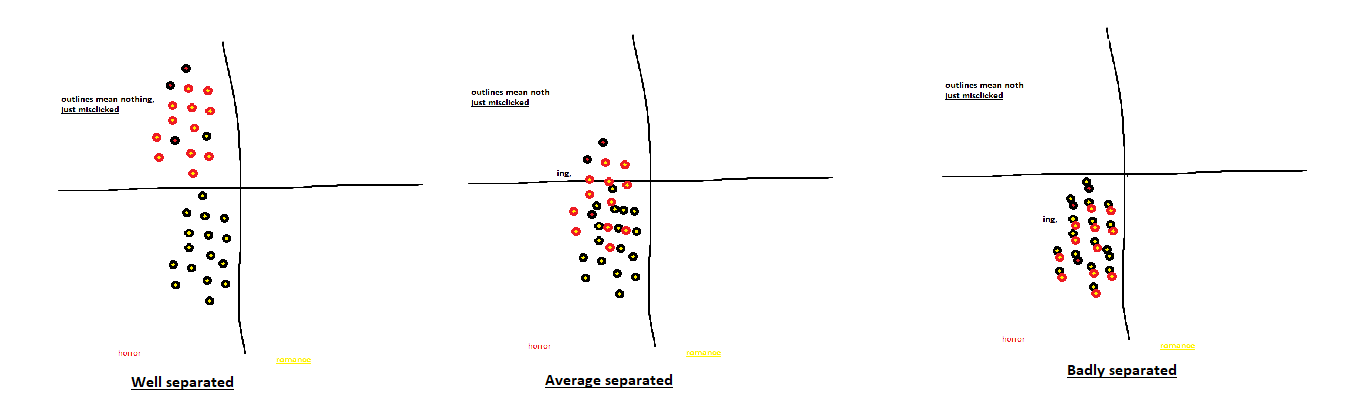
\includegraphics[width=\textwidth]{images/genres_separated.png}
%	\centering
%	\caption{A conceptual space of movies, where regions correspond to properties and entities are points.}\label{figure:genres_separated}
%\end{figure}

%The relationships in Vector Space Models can be extracted to obtain domain knowledge. %king and queen was parallel to the vector between prince and princess. % NEED TO MAKE THIS REAL



\begin{figure}[t]
	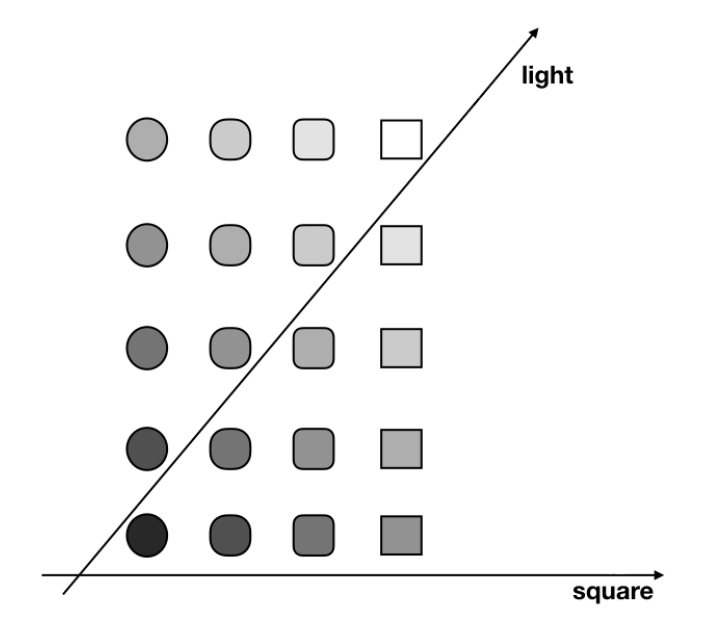
\includegraphics[width=250px]{images/toy_domain.png}
		\centering
	\caption{An example in a toy domain of shapes.}\label{ch3:ToyDirectionsGraphic}
\end{figure}

The simple linear classifiers that are used to evaluate the method's feature directions are low-depth Decision Trees. In Figure \ref{ch3:DecisionTree} an example is shown of a shallow Decision Tree using the method's interpretable representation. Shallow Decision Trees were chosen because they are effective at evaluating the disentanglement of the representations features. If the features are disentangled, then a low-depth Decision Tree will suffice to classify natural domain tasks. Shallow trees also evaluate the semantic generalizability of the features, as if they are able to classify complex classes using only a single feature then that feature must be semantically coherent and generalizable. In terms of interpretability, shallow trees have many positive effects for users, like lower response times \cite{Narayanan2018, Huysmans2011}, better question answering and confidence for logical problem questions \cite{Huysmans2011} and higher satisfaction \cite{Narayanan2018}. Although in this work  the superiority of  low-depth Decision Trees in real-world interpretability applications is not in the scope of the evaluation, as the interpretable representations  could be applied to a variety of classifiers.

The quantitative results for the method results show that the method can successfully disentangle a variety of representations even with trees as limited as depth one, and these shallow trees outperform the original representation greatly when compared to deeper trees on the uninterpretable original features. Additionally, the results in most cases are also competitive with Latent Dirchlet Allocation, a baseline interpretable topic model. The method is shown to be an effective way to obtain a disentangled representation that can effectively produce simple interpretable classifiers. The method is verified to work on five different representation types for five different domains, using natural domain tasks for those domains. 

\begin{figure}[t]
	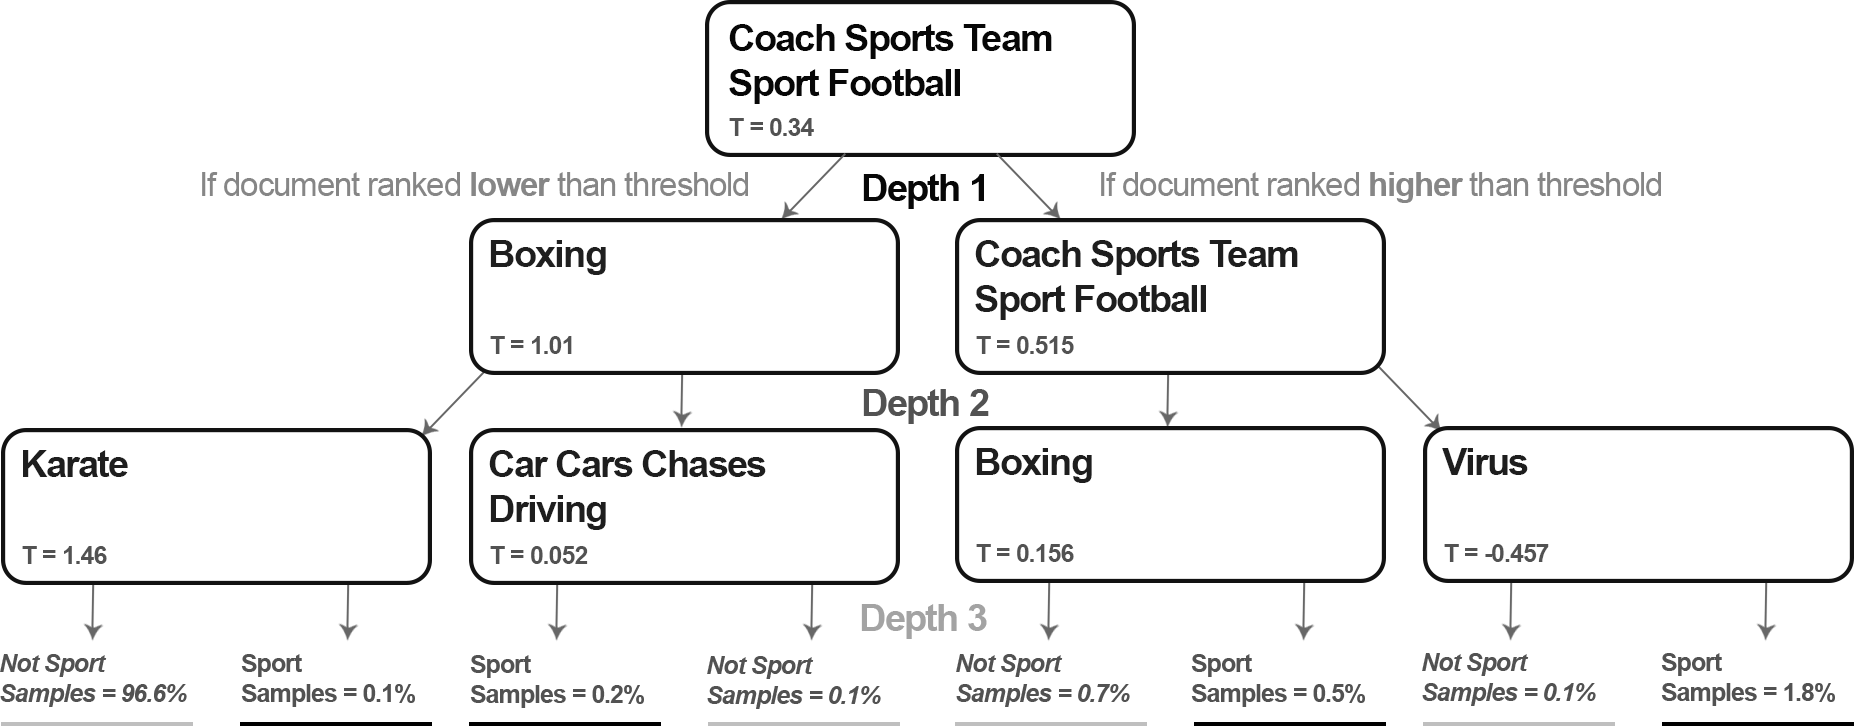
\includegraphics[width=450px]{images/decision_tree_ex.png}
	\centering
	\caption{An example of a Decision Tree classifying if a movie is in the "Sports" genre. Each Decision Tree Node corresponds to a feature, and the threshold T is equal to the ranking of a document on that feature. The most important direction is used twice, referring to sports and resulting in a majority of negative samples. The nodes at depth three are more specific, sometimes overfitting (e.g. in the case of the "Virus" node) }\label{ch3:DecisionTree}
\end{figure}


%Why interpretability for document classification matters:

%What Vector Space Models are there that perform well at tasks:

%What document classification tasks are important:

%What methods are there for interpretable document classification:

%Derrac \cite{Derrac2015} introduced an unsupervised method to go from a Vector Space Model and its associated Bag-Of-Words to a representation where each dimension is a ranking of documents on a feature of the domain. For example, in the domain of movie reviews genres would be a feature, and the dimension would have a numeric value for each document corresponding to the degree it is a particular genre. The contribution of this Chapter is an analysis and experimentation on the quality of these features applied to document classification. The main insight from our work is that these interpretable features do not suffer a performance drop in a non-linear classifier compared to the original representation, and can outperform the original representation and a baseline interpretable representation in a linear classifier. In addition, we find that if a dimension ranks documents on a feature relevant to the task, it can be competitive with more complex models using a single Decision Tree node. We show an example of the representation from a domain of IMDB movie reviews in \ref{ch3:TreeAndRep}. 

%\begin{figure}[t]
%	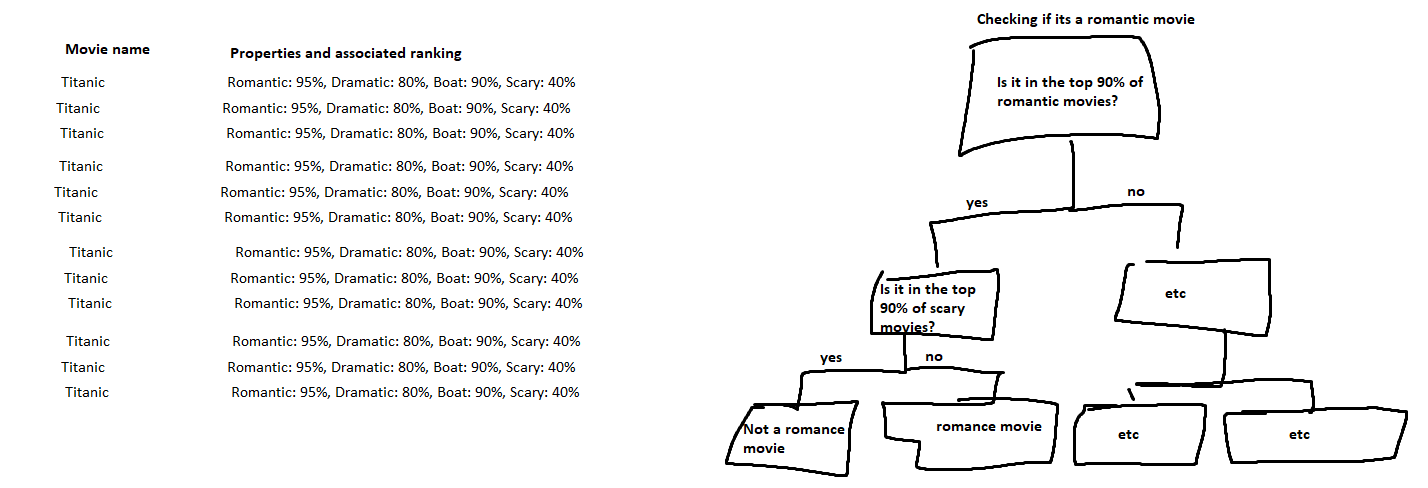
\includegraphics[width=\textwidth]{images/tree and rep.png}
%	\centering
%	\caption{Example movies and selected associated dimensions, chosen according to their relevance to the genre task.}\label{ch3:TreeAndRep}
%\end{figure}

%Vector Space Models encode semantic relationships

%What are the applications of semantic relationships? What is the power of a semantic relationship? Why are semantic relationships important in a space?
%prolly need more about

%What are directions? Why are directions important? What have they been used for? What is a feature direction?


% How can I apply directions to produce an interpretable space? Why is this valuable? What makes this interesting? What are feature rankings?


%%What are the advantages, disadvantages of the previous work?



%Why do this work? What is the value of this work?  How is this relevant to the readers interests?


%\subsection{Using a Property Representation in a Linear Classifier}


%Our method can use any vector space that linearly separates entities, and so it has potential longevity. This means that our method is relying on structure in the space that does not directly correspond to our desired representation -  we can view our approach as a linear transformation of the space. We address this problem in Chapter \ref{chapter:finetuning}. However, we have the capability to leverage many different methods to construct a vector space for our representation, so as long as dense representations of entities exist it will be possible to use our method, and as they are improved the results that our method can achieve will be improved too. This kind of flexibility also gives us the potential to combine the resultant representations from different vector spaces for classification, e.g. concatenating the vectors from different spaces.

%Topic models such as Latent Dirichlet Allocation (LDA) represent documents as multinomial distributions over latent topics, where each of these topics corresponds to a multinomial distribution over words \cite{Blei2003}. These topics tend to correspond to semantically meaningful concepts, hence topic models tend to be rather interpretable \cite{Chang2009}. To characterize the semantic concepts associated with the learned topics, topics are typically labelled with the most probable words according to the corresponding distribution. 

% What is a Vector Space Model? Why is a Vector Space Model valuable?




% 




%%What is the previous work?
 %What is a direction




%Finally, \cite{derracAIJ} found salient properties as direction vectors in a Vector Space Model of entities (e.g. Movies in a domain of IMDB movie reviews), and labelled them with clusters of words (e.g. $p_1 = {Scary, Horror, Gore}, p_2 = {Funny, Laughter, Hilarious}$).  We show a toy example in Figure \ref{ToyDirection}. %Copied from CONLL 




%%What is our contribution towards those disadvantages in this chapter?
%"Decision Trees, Decision Tables and Textual descriptions of rules are logically equivalent in the sense that one type of representation can be automatically translated to another (albeit in a simpler or more complex form), while preserving the predictive behaviour of the original model"


%%What are some real world scenarios that you could see our work taking effect in?
%In a case study by , giving the business users the option between a model with higher classification score but more input variables and a lower classification score but less input variables resulted in more buy-in for system designers. By accurately representing salient concepts in the domain, we are also able to offer a similar option; less nodes in the Decision Tree in exchange for more accuracy. % Potentially this citation sucks


%How is the work evaluated? How can you justify the evaluation? 
%%What are some alternative interpretable classifiers? What are some approaches to interpretable classification?

%%How does our work fit into the niche of interpretable classifiers?

%%What kind of tasks are these interpretable classifiers usually on? How do we compare in terms of evaluation?

%%How does our evaluation of interpretability play into our idea of interpretability outlined in Chapter 1?


The interpretable representation that is obtained by this method is composed of in terms of salient features, where each of these features is described using a cluster of natural language terms. This is somewhat similar to Latent Dirichlet Allocation (LDA), which learns a representation of text documents as multinomial distributions over latent topics, where each of these topics corresponds to a multinomial distribution over words \cite{Blei03latentdirichlet}.  Topics tend to correspond to salient features, and are typically labelled with the most probable words according to the corresponding distribution. On the other hand, our work leverages clustering methods to obtain the feature labels. Broadly speaking, in the context of document classification, the main advantage of topic models is that their topics tend to be easily interpretable, while Vector Space Models tend to be more flexible in the kind of meta-data that can be exploited e.g.\ they allow us to use neural representation learning methods to obtain these spaces. The approach proposed in this Chapter aims to combine the best of both worlds, by providing a way to derive interpretable representations from Vector Space Models.  Many extensions of LDA have been proposed to incorporate additional information as well, e.g.\ aiming to avoid the need to manually specify the number of topics \cite{teh2005sharing}, modelling correlations between topics \cite{Blei2006}, or by incorporating meta-data such as authors or time stamps \cite{rosen2004author,wang2006topics}. Nonetheless, such techniques for extending LDA offer less flexibility than neural network models, e.g.\ for exploiting numerical attributes or visual features. For comparison, in our experiments the standard topic model algorithm Latent Dirchlet Allocation (LDA) is used as a baseline to  compare to the new methodology that transforms standard Vector Space Model representations. %Topic Models are also entirely probabilistic, while our method relies entirely on the spatial relationships present in the vector space model.


There is much work on learning interpretable representations, with one popular way being to introduce sparsity or non-negativity constraints while learning, for example, sparse PCA learned using the l1-norm, \cite{H.Zou2006} \cite{Zhang2012},  or Non-Negative Sparse Embeddings (NNSE)  \cite{Murphy} which are sparse interpretable word-vectors obtained using sparse-matrix factorization and non-negativity constraints. A similar technique can also be applied to distributional word-embeddings by integrating this method with the Skip-Gram model \cite{Luo2015}. However, our approach is not intended to transform the learning processes, but rather be a post-processing step on an existing representation.

Similar to the approach in this chapter, \cite{Faruqui2015} introduce a post-processing method to convert any distributional word-vector into sparse word vectors, which additionally satisfy our idea of disentangled interpretability. However, the representation produced by the method in this work differs from sparse representations in that it is dense, where each feature is salient and interpretable. Another method is to describe a representation, e.g. sense word-embeddings that are linked to synsets \cite{Panchenko2016} in-order to make them interpretable. Although this is a post-processing step similar to our method, this is a linking rather than a transformation of the representation.  

Another method is to integrate grammatical structure into the learning of the representation, for example \cite{Liu2017} obtained a representation learned with attention mechanisms on the dependency structures of sentences, but this differs from the intention of our work, which is not to introduce new structures to the representation to make it more interpretable but instead use the already existing structure to obtain an interpretable representation. For short interpretable documents, \cite{Martinc} introduced tax2vec, which produced interpretable features from word taxonomies, useful for low data models. In \cite{Code} word-vectors were clustered and then used as a bag-of-clusters, where if a word occurs in those word-vector clusters it contributes to the Bag-Of-Words frequency. Although clustering is used in the method, it is not used to create a Bag-Of-Words, instead relying on the spatial relationships in the space as our representation. 

%How is the chapter going to play out? Whats going to happen?
%As our work performs well even at lower-depth trees, this gives potential users more flexibility in how they want to present the information, e.g. to a potential client. Compared to Bag-Of-Words, which loses its representation capabilities the lower the depth.

This chapter continues as follows: First the method is described, making explicit the variations from to the original method in \cite {Derrac2015}. This is followed by a qualitative  and quantitative analysis, finishing with a conclusion on the  benefits and limitations of this approach.



%\section{Related Work}
%Sparse word vectors
%Adapted to composition \cite{Fyshe2015}
%\subsection{Semantic Relations \& Their Applications}

%Our method uses the relationships inherent in a Vector Space Model. Other work has formalized the relationships found in Vector Space Models, for example in word-vectors, linear analogies (see Section \ref{WordVectors, Ethayarajh2018}, were found where the vector between  %Copy pasted from this 
%[ENTIRE SECTION COPY PASTED FROM PREVIOUS PAPER]
%\textbf{Linear Classifiers}
%Decision Trees, linear SVM's, logistic regression, decision tables, IF Then rules.

%What are the available options for interpretable linear classification?

%How have each of these methods been measured or validated in the literature in regards to interpretability? How about application to real world situations?

%\textbf{Non linear classifiers}
%What non linear classifiers networks are interpretable? How have they done it? How have they measured it? How does it compare to a linear method?

%\textit {Neural networks}Approximating w/linear model, Interpretable nodes/weights

%\textit {Other Stuff}

%\subsection{Interpretable Representations}


%There are two ways in which topic models can be used for document classification. First, a supervised topic model can be used, in which the underlying graphical model is explicitly extended with a variable that represents the class label \cite{Blei2010}. Second, the parameters of the multinomial distribution corresponding to a given document can be used as a feature vector for a standard classifier, such as a Support Vector Machine (SVM) or Decision Tree. .




% One of the more popular models for text representation that labels features in a similar way to our method are Topic Models.


\section{Method}\label{ch3:method}
% Assumed understanding at this point
% Chapter 1: Why interpretability is important. The value of a good interpretable representation. What directions are and what they mean.
% Chapter 2: The background and literature review for interpretable representations.
% Chapter 3: An introduction on the value of a good interpretable classifier, and the position of our work in that domain and how it can be applied there. What entities, properties are. What a conceptual space is. A literature review on relevant interpretable classifiers.

This section details the methodology to obtain an interpretable representation from only a Vector Space Model and its associated Bag-Of-Words \ref{bg:SemanticSpaces}. %which whose features rank documents on salient semantics, e.g. In a domain of IMDB movie reviews, a movie would be ranked on semantics like  $1: \{Scary, Horror, Bloody\}$ and $2: \{Romantic, Love, Cute\}$, ideally with as many rankings as salient semantics of the domain. 
%Make sure features ae explained well earlier 

%\subsection{The Structure of a Vector Space Model}

%Salient features of the domain are encoded in the structure of a Vector Space Model. 
% What are directions? How are they encoded? Why are they encoded that way?



 

%\begin{figure}[t]
%%	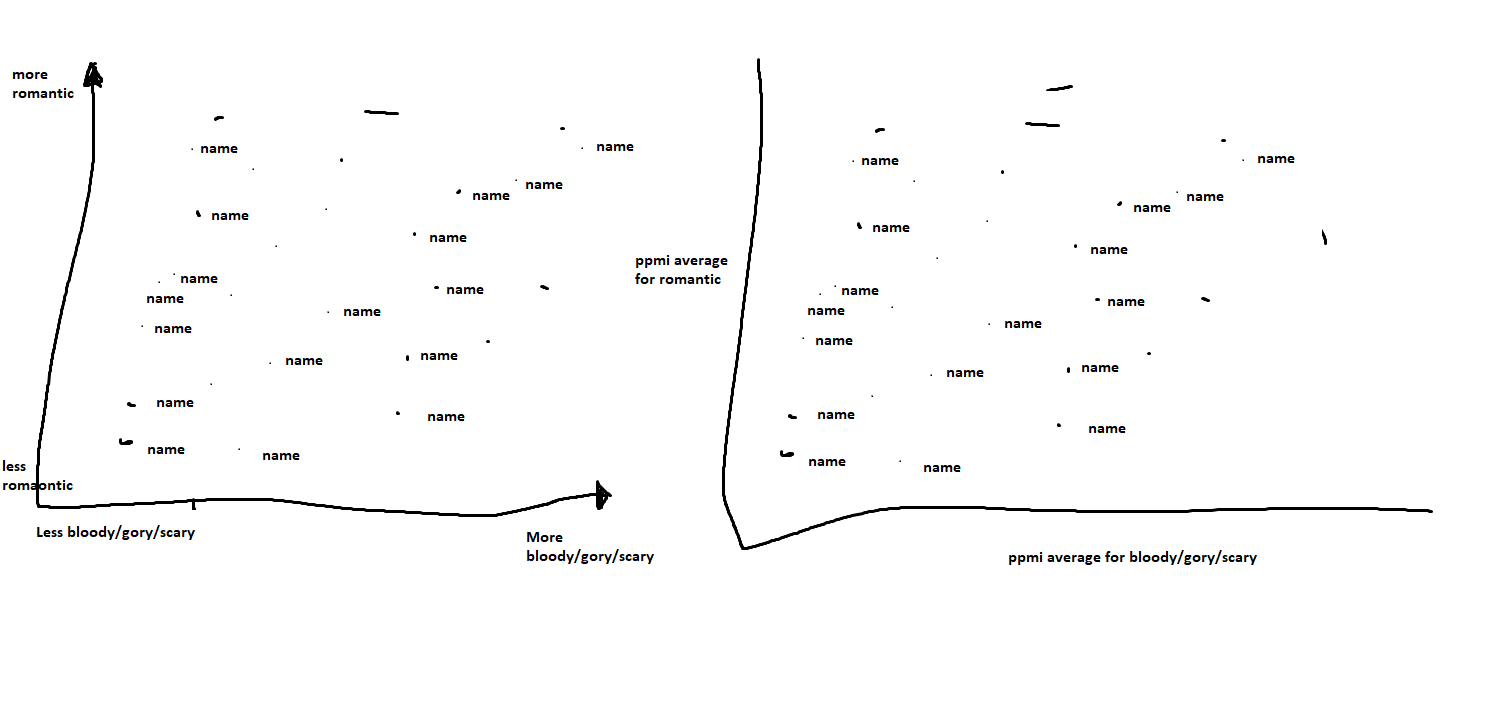
\includegraphics[width=\textwidth]{images/DirectionsGraphic.png}
%	\centering
%	\caption{Original And Converted.}\label{ch3:DirectionsGraphic}
%\end{figure}
%The method to obtain interpretable feature-vectors is an extension of the work by \cite{derracAIJ}. This previous work showed how to, filter out words, cluster words to get features, and obtain rankings of documents on those features. In this section, we further analyse and extend this work, in particular by testing a variety of additional filtering methods and clustering methods, and demonstrating how these feature-vectors can produce simple linear interpretable classifiers. 
%To begin, we filter out terms that will not be well represented in the space, and in-turn will not result in good feature rankings. We do so by first removing all terms below a frequency threshold. Then, for each word we obtain a direction in the space that can induce a ranking of documents on that word, and evaluate how well represented that word is in the space and remove those below a threshold. We can consider the terms remaining to be candidate feature-directions, as they are all well represented in the space and are unlikely to be highly scored as representative due to being infrequent. However, it is possible that they may not represent different information from each other, e.g. "blood" and "bloody" are likely quite similar. Additionally, we can understand that a good feature will not correspond directly to a term, but instead to a more abstract concept, e.g. "Blood, Gore, Horror". To obtain these more abstract feature-directions, and ensure the feature-directions are distinct rather than representing the same information, we cluster together similar feature-directions and obtain their feature-rankings to obtain our final representation. Each of these feature-rankings can be labelled with the cluster of words they are composed of. 



\subsection{Obtaining Directions and Rankings From Words}


We explain the method in terms of document classification.  Assuming a Bag-Of-Words $B_w $ has an associated vocabulary $W_w $, 
in this section we introduce the first step: how to obtain feature-directions $D_w $ for each word $W_w $, and rankings of documents  on these directions $r_w $, where each word is ranked on every document. For this step, not all words are expected to be salient in the domain. Instead, the first step shows how to obtain an interpretable representation where every document is ranked on every word, and the next step shows how to filter these rankings to only salient features.

%%%%%%%%%%%%Features that are important will be spatially organized in a way that reflects the similarity between the Bag-Of-Words representations they were composed of. In particular, we expect that documents will be arranged in a direction, where generally the higher the PPMI score for a group of words that correspond to a feature (e.g. $Horror, Scary, Gore$) the further away they will be from those that have low PPMI scores for those words. We give examples of this in Figure \ref{ch3:DirectionsGraphic}, by projecting documents into a 2D space of salient features we are able to show that these documents are structured according to directions for these features. Salient features will typically be a more abstract representation which will be natural in the domain, e.g. in a domain of IMDB movie reviews, genres

\noindent \textbf{Obtaining directions for each word} Each document is referred to as a point $d_p $ in the vector space model $S_{d}$. For each word $w$, a hyper-plane is obtained $h_w $ from a Linear Support Vector Machine (See Section \ref{bg:SVM}\footnote{This was also tested using a logistic regression classifier, and achieved similar results}) that is trained on the Bag-Of-Words representation so that document points $d_p $ in the space $V_d$  where the word $w $ occurred more than once  for that document $d_{wf} >= 1$ are separated from those where the word did not occur $d_{wf} == 0$. This process is repeated such that a hyper-plane is found for all words in the vocabulary above a frequency threshold $w_f > T$ where $T$ is chosen such that words which are infrequent enough to cause the classifier to overfit are not included. As this task is unbalanced, i.e. there are typically less documents that contain the word compared to those that do not contain it, the weights of the classifier are balanced such that positive instances are weighted in proportion to how rare they are. 

As previously mentioned, not all words will be influential on the structure of the representation. Only words that are salient will be well separated. Although the hyperplane $h_w$ learned is binary (either classifying documents $d_p$ as negative or positive), it can  be expected that the distance of the document points $d_p$ from the hyperplane boundary varies, as the space's $V_w$ similarity structure is in degrees rather than hard boundaries. For example in a space constructed from frequency vectors $W_{wf}$, it can be expected that the documents which contain the word more frequently would be further away from the hyper-plane on the positive side. Similarly, in the case of our experiments, the documents with a higher PPMI value will be more distant from the hyper plane on the positive side. This is the insight that informs the method to obtain the direction. 

The vector $v_w$ perpendicular to the hyperplane $h_w $ is taken as a direction $D_w $ that models documents $d_p$ from the lowest document ranked on the word $w $ (at the distance furthest from the hyperplane on the side where documents $d_p $ are classified) to the highest ranked on the word $w$ at the distance furthest from the hyperplane at the positive side. An example of such a direction $D_w$ is shown in the toy domain in Figure \ref{ch3:ToyHyperPlane}. To  apply this idea to a real domain, we can give an example from movie reviews, where the word is 'Scary' and the most 'Scary' movies are at the tip of the direction and those that are least 'Scary' are at the base of the direction.  %Although these directions do formally correspond to vectors, we refer to them as directions to emphasize their intended ordinal meaning: feature directions are aimed at ranking entities rather than e.g.\ measuring degrees of similarity. %Graphical representation of 


\begin{figure}[t]
	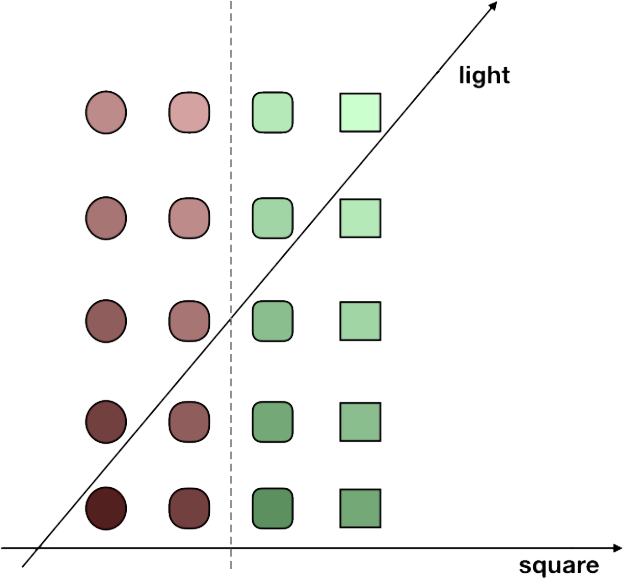
\includegraphics[width=250px]{images/ToyHyperplane.png}
	\centering
	\caption{An example of a hyper-plane and its orthogonal direction in a toy domain of shapes. Green shapes are positive examples and red shapes are negative examples, but despite the problem being binary those closest to the hyper-plane are less defined than those further away, resulting in the orthogonal vector being a direction}\label{ch3:ToyHyperPlane}
\end{figure}




\noindent \textbf{Ranking documents on directions} Although we do refer to the direction $D_w$ ranking documents on a word $w$, we do not yet have a specific value to represent this ranking. Once a feature-direction vector is obtained for each word $D_w$ the next step is to quantify the degree to which each document $d_p$ has that word, by obtaining a value that corresponds to how far-up it is on the direction vector $D_w$.  If $d_p$ is the representation of a document in the given vector space as a point then the dot product is used between the direction vector for the word $D_w $ and the document vector $D_w \cdot p_d$ as the ranking $r_{dw}$ of the document $d$ for the word $w$, and in particular, we take $r_{d1} < r_{d2}$ to mean that the document $d_2$ 'has' the feature  to a greater extent than $d_1$ (e.g. in a domain of movie reviews if the word is 'cinematography', the movie will likely have notable cinematography). Once the dot product value is obtained in this way for each document on a word, this forms a ranking feature for the word.  By obtaining a ranking of all documents on all words,  a rankings matrix of size $d_n * w_n $ can be obtained. This representation forms the basis of the method, with future steps removing those directions that are not salient, and then clustering similar directions together. %To give an understanding of these rankings and their saliency, we show some examples of features and documents ranked on them for different domains with varying degrees of saliency. In the next section, we show how we measure the saliency of directions and filter those that are not salient out of the representation. %Graphical representation of entities being ranked on a direction vector






%\begin{figure}[t]
%	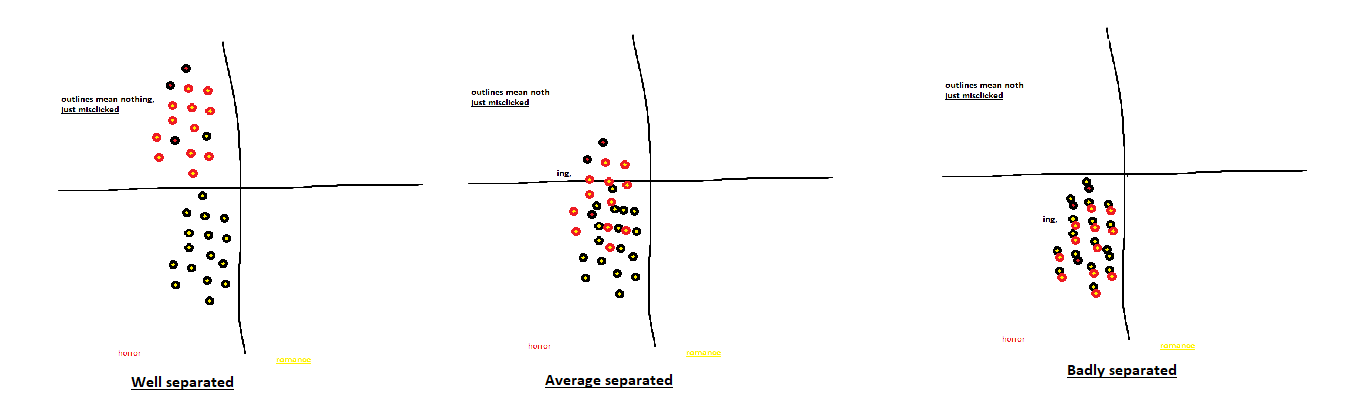
\includegraphics[width=\textwidth]{images/genres_separated.png}
%	\centering
%	\caption{Original And Converted.}\label{ch3:OrigAndConverted}
%\end{figure}



\subsection{Filtering Words}

%With the rankings $R_r$, we could create a representation of each document $d$, composed of $w_n$ dimensions, where each dimension is a ranking of the document $d$ on that word $r_dw$. However, many of the words are not spatially important enough in the representation to result in a quality ranking - they are not salient features.

In this section, words are filtered that do not influence the structure of the domain. This is done by evaluating them using a scoring metric, and removing the words that are not sufficiently well scored. Originally, only binary features were considered. These binary features were measured  in terms of the performance of the SVM classifier.  If the hyperplane correctly separates the entities well, it must mean that whether word $w$ relates to document $d$ (i.e.\ whether it is used in the description of $d$) is important enough to affect the Vector Space Model representation of $d$.  However, this approach does not consider the quality of the ranking. To consider this, the new metric Normalized Discounted Cumulative Gain was introduced, using the bag-of-words as its target ranking under the assumption that if a ranking matches the ordered score of a PPMI BOW, then it is a good ranking. If this is the case, it can also be assumed that this means the word was strongly influential in the space, as it retains the detail of the Bag-Of-Words information in the space's structure. 

\noindent

\noindent \textbf{Cohen's Kappa}. This is the metric used in the work that originally introduced this method \cite{Derrac2015}. This is a binary feature evaluation metric that deals with the problem that these words are often very imbalanced. In particular, for very rare words, a high accuracy might not necessarily imply that the corresponding direction is accurate. For this reason, they proposed to use Cohen's Kappa score instead. In our experiments, however, it was found that this can be too restrictive, allowing us to sometimes obtain better results with the more simple accuracy metric.\smallskip %This is basically copy pasted.


 \textbf{Classification accuracy}. If a model has high accuracy for a word $w$, it seems reasonable to assume that $w$ describes a salient property for the given domain. However, despite balancing the weights of the original SVM used to obtain the hyper-plane, the value this metric places on correctly predicting negative classification often results in noise particular to this metric being identified, e.g. metadata like a reviewers name that only occurs in a few reviews being given a high accuracy score as the method, as it overfit to only predict negative instances.%This is basically copy pasted.
\smallskip


\noindent \textbf{Normalized Discounted Cumulative Gain} % MATHEMATICS NEEDS TO BE REWRITTEN
This is a standard metric in information retrieval which evaluates the quality of a ranking w.r.t.\ some given relevance scores \cite{jarvelin2002cumulated}. It favours initial documents over later ones.  Some alternative metrics were tried that did not prioritize the top rankings being correct more, but this came with two problems. First, PPMI has a large number of zero scores. This makes the lower dot product documents have an uneven comparison, disrupting the score based on them being given a non-zero ranking score by the method. The second is that the documents without many occurrences of the word are less prioritized in the space, and largely influenced by other words, making their ranking less reliable.  In our case, the rankings $r_d$ of the document $d$ are those induced by the dot products $v_w \cdot d$ and the relevance scores are determined by the Pointwise Positive Mutual Information (PPMI) score $\textit{PPMI}(w,d)$, of the word $w$ in the BoW representation of entity $d$ where
$\textit{PPMI}(w,d) = \max \big(0, \log\big(\frac{p_{wd}}{p_{w*} \cdotp p_{*d}}\big)\big)$, and
\begin{align*}
p_{wd} &= \frac{n(w, d)}{\sum_{w'} \sum_{d'} n(w', d')}
\end{align*}
where $n(w,d)$ is the number of occurrences of $w$ in the BoW representation of object $d$, $p_{w*} = \sum_{e'} p_{wd'}$ and $p_{*d} = \sum_{w'} p_{w'd}$. %This is basically copy pasted.
\smallskip

By scoring the words on these features, a simple cut-off is applied (e.g. the top 2000 scored words) to obtain the most salient words. Ideally, this cut-off would be at the point where the words stop corresponding to salient features. However, it is difficult to determine this, so in practice this value is taken as a hyper-parameter.

In principal, NDCG should be better suited for gradual features. In practice, however, there was not such a clear pattern in the differences between the words chosen by these metrics despite often finding different words. Put another way, it is difficult to say if the words highly scored by NDCG are more gradual than other scoring metrics.%We show the top scoring terms found by each scoring type below in Table \ref {X}.

\subsection{Labelling Words}\label{ch3:LabellingWords}
Although the rankings of single words are informative for models, it is difficult for a human to grasp the meaning of a word without context. This can be resolved simply by finding the $n$ most similar directions to each word's direction.

Another approach is to use a clustering method like k-means. For these clustering method, the aim is to go from single word directions $D_w$ to clusters of these single word directions $C_d$ labelled by the words clustered together $C_w$.
If we consider two directions, "Blood" and "Gore", both of these are approximating a similar feature of movies, they both relate to how much blood a movie contains. Because of this, their directions will be very similar to each other. This is the first idea behind using a clustering method on these directions. It  resolves the issue of repetition in the directions, and if the clustered directions are averaged then that clustered direction will balance between documents that used the word 'Bloody' to describe the bloodiness of the movie and the word 'Gore'. Some films may be 'Bloody', but may not necessarily have the term 'Gore' in their reviews, and vice versa. Or, a review may favour one term over the other. By using a clustering method, a direction could be obtained that more accurately represents the semantics of a bloody film more than either of the terms individually. 

It is not always the case that this new clustered direction will perform better than a single relevant direction for a class. In fact, its possible that when clustering many terms together, the ranking can be more disrupted than helped. For example given a cluster  $\{Romance, Love\}$ and a cluster $\{Blood, Gore\}$ the direction for $\{Cute\}$ is clearly more relevant to the former rather than the latter, and likely has been used in the reviews for romance movies. But it has also likely been used in reviews for movies containing cute animals. This would make the new clustered direction $\{Romance, Love, Cute\}$ perform worse at classifying the movie genre "Romance", but a bit better at classifying animal movies. Ideally, this feature would form a new cluster - but a balance must be held between retaining the precision of the rankings and introducing new rankings that are appropiately disentangled from the existing ones, without repeating existing concepts. In the quantitative results, sometimes clustering performed worse than single directions, and not being able to find this balance for the specific classes in question can be attributed as to why.
%What are we doing with clustering
 %Similarly, obtaining a hyper plane using a Logistic Regression classifier that uses occurences of both and either of these terms as positive would be similar to this averaged direction.

% When is clustering useful? When does clustering outperform single directions? When are single directions useful?

%What is the value of a cluster label?


%The final benefit to clustering the words is that linear classifiers are generally suited better to 'disentangled' representations \cite{Bengio2012}. In this case, we refer to disentanglement in the sense of obtaining a feature vector where each dimension is distinct, rather than the Vector Space Model being naturally clustered. Additionally, if our representation is dense and disentangled into the natural features of the domain, it is unlikely to overfit and will be able to generalize more easily. 

The previous work's clustering method is used, and additionally k-means is experimented with:

\noindent \textbf{Derrac's K-Means Variation} This is the clustering method used in the work this method was introduced in \cite{derrac2015}. As input to the clustering algorithm, it considers the $N$ best-scoring candidate feature directions $v_w$, where $N$ is a hyperparameter. The main idea underlying their approach is to select the cluster centers such that (i) they are among the top-scoring candidate feature directions, and (ii) are as close to being orthogonal to each other as possible. 
 
The output of this step is a set of clusters $C_1,...,C_K$, where each cluster $C_j$ is identified with a set of words.
Furthermore  $v_{C_j}$ will be written to denote the centroid of the directions corresponding to the words in the cluster $C_j$, which can be computed as $v_{C_j}= \frac{1}{|C_j|} \sum_{w_l\in C_j} v_l$ provided that the vectors $v_w$ are all normalized. These centroids $v_{C_1},...,v_{C_k}$ are the feature directions that are identified by the method. 

The first cluster centroid is chosen by taking the top-scoring direction for its associated metric. Then, centroids are selected until the desired amount is reached by taking the maximum of the summed absolute cosine similarity of all current centroids, in other words taking the most dissimilar direction to all of the current directions. Once the centroids are selected, for each remaining direction the centroid is found it is most similar to, and the centroid is updated once the direction has been added. 

Cluster centroids are taken as cluster directions, and the representation is obtained by ranking documents on this cluster direction. It is also possible to rank documents on the initial direction only, and use the cluster names as descriptions if the clusters are too noisy.

\noindent \textbf{K-Means} Although the previous method does have a method for selecting cluster centres, typically it was found that it relies too much on its initial directions, meaning if a noisy direction is chosen as the first cluster centre, then key directions may be missed. Avoiding this is difficult without extensive and sometimes arbitrary hyper-parameter optimization. For this reason, it was decided to try K-Means as a clustering algorithm. K-means traditionally begins with $K$ centroids $c$ randomly placed into the space. In our case, these centers are weighted according to the squared distance from the closest center already chosen. \cite{Arthur} %This intialization is improved by XXX method.  
Then, the distance between each point $d_p$ and centroid $c$ is calculated. In-order for euclidian distance to be meaningful, directions are normalized making euclidian distance the same as cosine similarity. Each point $p$ is then assigned to its closest centroid $c$. Then, the centroids are recomputed to be the mean of their assigned points. This process starting with the distance calculation is repeated until the points assigned to the centroids do not change. 

%We show some examples of clusters from each of these methods in Table \ref {XY}.

%Although we are able to find the words that are most salient, the best features in the domain may not correspond directly to words. Further, the features may not be well described by their associated word. In-order to find better representations of properties, we cluster together similar vectors $v_w$, following the assumption that those vectors which are similar are representing some property more general than their individual words, and we can find it between them.

%As the final step, we cluster the best-scoring candidate feature directions $v_w$. Each of these clusters will then define one of the feature directions to be used in applications. The purpose of this clustering step is three-fold: it will ensure that the feature directions are sufficiently different (e.g.\ in a space of movies there is little point in having \emph{funny} and \emph{hilarious} as separate features), it will make the features easier to interpret (as a cluster of terms is more descriptive than an individual term), and it will alleviate sparsity issues when we want to relate features with the BoW representation, which will play an important role for the fine-tuning method described in the next section.


%Table \ref{tabKappaNDCG} displays some examples of clusters that have been obtained for three of the datasets that will be used in the experiments, modelling respectively movies, place-types and newsgroup postings. For each dataset, we used the scoring function that led to the best performance on development data(see Section \ref{secExperiments}). Only the first four words whose direction is closest to the centroid $v_C$ are shown.
%\noindent \textbf{K-Means}
%\noindent \textbf{Derrac's K-Means Variation}
%\noindent \textbf{Mean-shift}
%\noindent \textbf{Hdbscan}

%Our overall aim is to find directions in the Vector Space Model that model salient features of the considered domain. For example, given a Vector Space Model of movies, we would like to find a direction that models the extent to which each movie is scary, among others. Such a direction would then allow us to rank movies from the least scary to the most scary. We will refer to such directions as \emph{feature directions}. Formally, each feature direction will be modelled as a vector $v_f$. However, we refer to \emph{directions} rather than \emph{vectors} to emphasize their intended ordinal meaning: feature directions are aimed at ranking objects rather than e.g.\ measuring degrees of similarity. 

\section{Qualitative Results}

\subsection{Datasets}\label{ch3:datasets}

The experiments are using five different domains. To begin, the properties of these domains are explained to try to give an insight into the kind of text stored within them. This is to better inform analysis of our qualitative results. Examples are shown in three domains in Table \ref{ch3:TextExamples}.

\begin{table}[] 
	\scriptsize
	\begin{tabular}{lp{6.75cm}p{6.75cm}}
		Data Type  & Unprocessed                                                                                                                                                                                                                                                                                                                                                                               & Processed       \\
		\midrule[\heavyrulewidth]
		Newsgroups & morgan and guzman will have era's 1 run higher than last year, and  the cubs will be idiots and not pitch harkey as much as hibbard.  castillo won't be good (i think he's a stud pitcher)                                                                                                                                                                                                & morgan guzman eras run higher last year cubs idiots pitch harkey much hibbard castillo wont good think hes stud pitcher                            \\
		Sentiment  & All the world's a stage and its people actors in it--or something like that. Who the hell said that theatre stopped at the orchestra pit--or even at the theatre door? 
		Why is not the audience participants in the theatrical experience, including the story itself?<br /><br />This film was a grand experiment that said: "Hey! the story is you and it 
		needs more than your attention, it needs your active participation"". ""Sometimes we bring the story to you, sometimes you have to go to the story.""<br /><br />Alas no one listened, 
		but that does not mean it should not have been said." & worlds stage people actors something like hell said theatre stopped orchestra pit even theatre door audience participants
		theatrical experience including  story film grand experiment said hey story needs attention needs active participation sometimes bring story sometimes go story alas one listened mean
		said \\
		Reuters    & U.K. MONEY MARKET SHORTAGE FORECAST REVISED DOWN The Bank of England said it had revised its forecast of the shortage in the money market down to 450 mln stg before taking account of its morning operations. At noon the bank had estimated the shortfall at 500 mln stg.                                                                                                               & uk money market shortage forecast revised bank england said revised forecast shortage money market 450 mln stg taking account morning operations noon bank estimated shortfall 500 mln stg     \\
		
	\end{tabular}
	\caption{Text examples from the first three domains}\label{ch3:TextExamples}
\end{table}

\textbf{20 Newsgroups\footnote{http://qwone.com/~jason/20Newsgroups/}} Obtained from scikit-learn. \footnote{https://scikit-learn.org/0.19/modules/generated/sklearn.datasets.fetch\textunderscore20newsgroups.html\#sklearn.datasets.fetch\textunderscore20newsgroups} Where documents are discussions from one of twenty different groups, specifically Atheism, Computer Graphics, Microsoft Windows, IBM PC Hardware, Mac Hardware, X-Window (GUI Software), Automobiles, Motorcycles, Baseball, Hockey, Cryptography, Electronics, Medicine, Space, Christianity, Guns, The Middle East, General Politics and General Religion. These also act as the classes for the dataset. Originally containing 18,846 documents, in this work it is preprocessed using sklearn to remove headers, footers and quotes. Then, empty and duplicate documents are removed, resulting in 18302 documents. The vocabulary size (unique words) is 141,321. The data is not shuffled. After filtering out terms that did not occur in at least two documents, ending up with a vocabulary of size 51,064. The number of positive instances averaged across all classes is 942, around 5\%.

\textbf{IMDB Sentiment} Obtained from Keras \footnote{https://keras.io/datasets/} Where documents are IMDB movie reviews, containing 50,000 documents with a vocabulary size of 78588. After removing terms that did not occur in at least two documents, ending up with a vocabulary of size 55384. This is a smaller change than the newsgroups, which began with a larger vocabulary than sentiment, but ended vocabularies about the same. This means that newsgroups contained many terms that were not relevant to a majority of the documents, likely because the 20 different newsgroups spread across so many topics. The corpus is split half and half between positive and negative reviews, with the task being to identify the sentiment of the review, so the number of positive instances in the classes is 25,000.

\textbf{Reuters-21578, Distribution 1.0} Obtained from NLTK\footnote{https://www.nltk.org/book/ch02.html}. Documents from the Reuters financial newswire service in 1987,  originally containing 10788 documents. After removing empty and duplicate documents, ending up with 10655 documents. It originally contained 90 classes, but as they were extremely unbalanced all classes that did not have at least 100 positive instances were removed, resulting in 21 classes. These classes are Trade, Grain, Natural Gas (nat-gas), Crude Oil (crude), Sugar, Corn, Vegetable Oil (veg-oil), Ship, Coffee, Wheat, Gold, Acquisitions (acq), Interest, Money/Foreign Exchange (money-fx), Soybean, Oilseed, Earnings and Earnings Forecasts (earn), BOP, Gross National Product (gnp), Dollar (dlr) and Money-Supply.   The original vocabulary size is 51,0001, and after removing all words that do not occur in at least two documents, the vocabulary size is 22542. The number of positive instances averaged across all classes is 541, around 5\%. 

\textbf{Placetypes} Taken from work by Derrac \cite{Derrac2015}. Documents are composed of concatenated flickr tags, where each document, named after a flickr tag, is composed of all flickr tags where that tag occurred. A minimum of 1,000 photos for each tag was a requirement, and the tags selected were taken from three different taxonomies (Geonames, Foursquare and the site category for the common-sense knowledge base OpenCYC).  It originally has a vocabulary size of 746,527 and 1383 documents. This is a very large vocabulary size to document ratio. The end vocabulary for this space was 100,000, which is used as a hard limit. This is roughly equivalent to removing all documents that would not be in at least 6 documents. As most classes in this domain are extremely sparse (less than 100 positive instances) no classes are deleted. There are three tasks, generated from three different place type taxonomies. The Foursquare taxonomy, classifying the 9 top-level categories from Foursquare in September 2013, Arts and Entertainment, College and University, Food, Professional and Other Places, Nightlife Spot, Parks And Outdoors, Shops and Service, Travel and Transport and Residence. the GeoNames taxonomy where 7 of 9 categories were used, Stream/Lake, Parks/Area, Road/Railroad, Spot/Building/Farm, Mountain/Hill/Rock, Undersea, and Forest/Heath. The OpenCYC Taxonomy, where 93 categories were used by Derrac, but it was only possible to match 25 of those classes to the representations. As 8 of these remaining classes had a low number of positive occurrences, OpenCYC classes are removed that do not have positive instances for at least 30 documents, leaving us with 17, Aqueduct, Border, Building, Dam, Facility, Foreground, Historical Site, Holy Site, Landmark, Medical Facility, Medical School, Military Place, Monsoon Forest, National Monument, Outdoor Location, Rock Formation, and Room. Naturally as these tasks were derived from taxonomies they are multi-label.

\textbf{Movies} Taken from work by Derrac \cite{Derrac2015}. A dataset where each document is a movie represented by all of its reviews concatenated across a number of sources (Rotten Tomatoes, IMDB, Amazon Reviews). It starts off with a vocabulary size of 551,080 and a document size of 15,000. However, after investigating the data made available by the authors, it was found that there were a number of duplicate documents. After removing these duplicate documents, there are 13978 documents. In the same way as the place-types, the vocabulary is limited at size 100,000. Three tasks are used to evaluate, 23 movie genres, specifically Action, Adventure, Animation, Biography, Comedy, Crime, Documentary, Drama, Family, Fantasy, Film-Noir, History, Horror, Music, Musical, Mystery, Romance, Sci-Fi, Short, Sport, Thriller, War, Western. 100 of the most common IMDB plot keywords (See Appendix \ref{app:ClassNames}) and Age Ratings from the UK and US, USA-G, UK-12-12A, UK-15, UK-18, UK-PG, USA-PG-PG13, USA-R.


 For each domain, we filter out terms that do not occur in at least two documents, and additionally limit the maximum number of words in a vocabulary to 100,000. For all of these datasets, we split them into a 2/3 training data, 1/3 test data split. We additionally remove the end 20\% of the training data and use that as development data for our hyper-parameters, which is then not used for the final models verified using test data.  For the movies and place-type domains, the original text was not available.



\subsection{Space Types}

Below the choices for the Vector Space Models that are formally described in Section \ref{bg:SemanticSpaces} are explained:

\textbf{Multi-Dimensional Scaling (MDS)}: Following \cite{derracAIJ}, we use Multi-Dimensional Scaling (MDS) to learn semantic spaces from the angular differences between the PPMI weighted BoW vectors. %A non-linear transformation that is used to evaluate the quality of representations when built from a standard BOW-PPMI. Chosen as it performed well in the work introducing this method.

\textbf{Principal Component Analysis (PCA)}: directly uses the PPMI weighted BoW vectors as input, and which avoids the quadratic complexity of the MDS method. A standard dimensionality reduction technique, used as a baseline reference.

\textbf{Doc2Vec (D2V)}: Inspired by the Skipgram model \cite{DBLP:conf/icml/LeM14}.  A distributional document representation used as a representative of a higher performing method of learning in terms of document classification. For the Doc2Vec space, the hyper-parameters are additionally tuned for the $window size (5, 10, 15)$ referring to the context window, the $min count (1, 5, 10)$ referring to the minimum frequency of words and the $epochs (50, 100, 200)$ of the network for each size space. The process with our two-part hyperparameter optimization as in this case is as follows: Grid search is used to select the parameters for the representation, then find the most suitable model (e.g. Decision Tree, SVM) for that representation. 

\textbf{Average Word Vectors (AWV)}: Finally, we also learn semantic spaces by averaging word vectors, using a pre-trained GloVe word embeddings trained on the Wikipedia 2014 + Gigaword 5 corpus\footnote{\url{https://nlp.stanford.edu/projects/glove/}}. While simply averaging word vectors may seem naive, this was found to be a competitive approach for unsupervised representations in several applications \cite{DBLP:conf/naacl/HillCK16}. We simply average the vector representations of the words that appear at least twice in the BoW representation.


\subsection{The best-performing directions for each domain}

To give an understanding of the kind-of directions found for each domain, the top-scoring ones are presented in Table \ref{ch3:TopScoringQua}. These are arranged from highest scoring to least scoring, with the score-type and space-type chosen by performance. These are not clusters, but rather single directions with the two most similar directions in brackets beside them for context. This is the alternative way of presenting these directions as mentioned at the start of Section \ref{ch3:LabellingWords}. 

There is an  interesting difference between the sentiment directions and the movies directions in the examples below. Both of these domains are composed of movie reviews, but the documents in the former are a concatenation of a number of reviews across different sources, while the latter are individual reviews. This has resulted in the more general concepts that apply to many movies being salient in the movies domain, but are less important than the names of actors and actresses in the sentiment domain. This is likely because the PPMI scores for actor names would be high as they are both rare and definitive for movies. For the newsgroups domain, a number of directions  are seen that are likely to only belong to a certain newsgroups, e.g. you would find the word 'celestial' more often in the religious sections than the others, and the word 'diesel' more often in the automobile section but not others. This is an expected natural clustering of the domain into its 20 newsgroups. The place-types section generally describes either aspects of the camera (e.g. canon60d), aspects of the photo (greyscale) or features found in the photo (gardening). The former likely relates to the degree to which filters or editing has been applied to the photo, while the latter makes more sense for our classification task. For the reuters dataset, the highest scored semantics seem to generally be related to dates (1st, may, june), however there is also some business jargon (quarterly, avg, dlr). 

\begin{landscape}
	\begin{table}[]
		\scriptsize
		\begin{tabular}{lllll}
			\textbf{Movies} \textit{(50 MDS NDCG)}        & \textbf{Sentiment} \textit{(100 D2V NDCG)}   & \textbf{Newsgroups} \textit{(50 D2V NDCG)} 			  & \textbf{Place-types} \textit{(50 PCA Kappa)}	 						 & \textbf{Reuters} \textit{(200 MDS NDCG)}       \\
			horror (scares, scary)               & glenda (glen, matthau)         & karabag (iranian, turkiye)                 & blackcountry (listed, westmidlands)     & franklin (fund, mthly)            \\
			hilarious (funniest, hilarity)       & scarlett (gable, dalton)       & leftover (flaming, vancouver)              & ears (stare, adorable)                  & quarterly (shearson, basis)       \\
			bollywood (hindi, india)             & giallo (argento, fulci)        & wk (5173552178, 18084tmibmclmsuedu)        & spagna (espanha, colores)               & feb (28, splits)                  \\
			laughs (funnier, funniest)           & bourne (damon, cusack)         & 1069 (mlud, wibbled)                       & oldfashioned (winery, antiques)         & 22 (booked, hong)                 \\
			jokes (gags, laughs)                 & piper (omen, knightley)        & providence (norris, ahl)                   & gardening (greenhouse, petals)          & april (monthly, average)          \\
			comedies (comedic, laughs)           & casper (dolph, damme)          & celestial (interplanetary, bible)          & pagoda (hindu, carved)                  & sets (principally, precious)      \\
			hindi (bollywood, india)             & norris (chuck, rangers)        & mlud (wibbled, 1069)                       & artificial (saturation, cs4)            & 16 (creditor, trillion)           \\
			war (military, army)                 & holmes (sherlock, rathbone)    & endif (olwm, ciphertext)                   & inner (curved, rooftops)                & 1st (qtr, pennsylvania)           \\
			western (outlaw, unforgiven)         & rourke (mickey, walken)        & gd3004 (35894, intergraph)                 & celebrate (festive, celebrity)          & 26 (approve, inadequate)          \\
			romantic (romance, chemistry)        & ustinov (warden, cassavetes)   & rtfmmitedu (newsanswers, ieee)             & vietnamese (ethnic, hindu)              & 23 (offsetting, weekly)           \\
			songs (song, tunes)                  & scooby (doo, garfield)         & eng (padres, makefile)                     & cn (elevated, amtrak)                   & prior (recapitalization, payment) \\
			sci (science, outer)                 & doo (scooby, garfield)         & pizza (bait, wiretap)                      & mannequin (bags, jewelry)               & avg (shrs, shr)                   \\
			funniest (hilarious, funnier)        & heston (charlton, palance)     & porsche (nanao, mercedes)                  & falcon (r, 22)                          & june (july, venice)               \\
			noir (noirs, bogart)                 & homer (pacino, macy)           & gebcadredslpittedu (n3jxp, skepticism)     & jewish (monuments, cobblestone)         & march (31, day)                   \\
			documentary (documentaries, footage) & welles (orson, kane)           & scsi2 (scsi, cooling)                      & canon60d (kitlens, 600d)                & regular (diesel, petrol)          \\
			animation (animated, animators)      & frost (snowman, damme)         & playback (quicktime, xmotif)               & reflective (curved, cropped)            & 4th (qtr, fourth)                 \\
			adults (adult, children)             & streisand (bridget, salman)    & 35894 (gd3004, medin)                      & mason (edward, will)                    & 27 (chemlawn, theyre)             \\
			creepy (spooky, scary)               & davies (rhys, marion)          & diesel (volvo, shotguns)                   & aerialview (manmade, largest)           & 14 (borrowing, borrowings)        \\
			gay (gays, homosexuality)            & cinderella (fairy, stepmother) & evolutionary (shifting, hulk)              & shelf (rack, boxes)                     & 11 (chapter, ranged)              \\
			workout (intermediate, instruction)  & boll (uwe, belushi)            & techniciandr (obp, 144k)                   & monroe (raleigh, jefferson)             & may (probably, however)           \\
			thriller (thrillers, suspense)       & rochester (eyre, dalton)       & 8177 (obp, 144k)                           & litter (fujichrome, e6)                 & 38 (33, strong)                   \\
			funnier (laughs, funniest)           & edie (soprano, vertigo)        & shaw (medicine, ottoman)                   & streetlights (streetlamp, headlights)   & m1 (m2, m3)                       \\
			suspense (suspenseful, thrillers)    & scarecrow (zombies, reese)     & scorer (gilmour, lindros)                  & carlzeiss (f2, voigtlander)             & dlr (writedown, debt)             \\
			arts (hong, chan)                    & kramer (streep, meryl)         & xwd (xloadimage, openwindows)              & manmade (aerialview, below)             & five (years, jones)               \\
			christianity (religious, religion)   & marty (amitabh, goldie)        & ee (275, xloadimage)                       & demolished (neglected, rundown)         & bushels (soybeans, ccc)           \\
			musical (singing, sing)              & columbo (falk, garfield)       & com2 (com1, v32bis)                        & wald (berge, wildflower)                & revs (net, 3for2)                 \\
			gore (gory, blood)                   & kidman (nicole, jude)          & examiner (corpses, brass)                  & arquitetura (exposition, cidade)        & 29 (175, include)                 \\
			animated (animation, cartoon)        & juliet (romeo, troma)          & migraine (ama, placebo)                    & greyscale (highcontrast, monochromatic) & acquisition (make, usairs)        \\
			gags (jokes, slapstick)              & garland (judy, lily)           & parliament (parliamentary, armored)        & alameda (monday, marin)                 & payable (div, close)              \\          
			
		\end{tabular}
		\caption{The top-scoring words for each domain, scoring metric and space type determined by the highest F1-score}\label{ch3:TopScoringQua}
	\end{table}
\end{landscape}





\subsection{Comparing Space Types}

To select these quantitative examples for  comparing score types, it was first demonstrated on the movies domain to be consistent with previous examples. However, as this does not contain the doc2vec space, additional results are provided in the next section for the newsgroups. The space that performed well on the genres task for the movies is used, with the understanding that genres as a key natural classification task will likely give good example directions that correspond to domain knowledge. After selecting this space, the same sized spaces are chosen from the other space-types (size 200). The same score-type and frequency cut-off  as the best performing space-type are also used. In this case, the best performing type for the PCA space was 20,000 frequency cutoff and NDCG. So even though sometimes a different frequency cut-off performed better for the other space-types, this is equalized so that the words are the same. This means that sometimes the space-type is  a slightly worse performing one than chosen as the final results, and that the original space has a performance advantage, but this makes the results more consistent. These qualitative experiments are approached with the following idea: spaces that perform better on natural domain tasks using Decision Trees contain unique natural directions that other spaces do not have. 

The commonalities between spaces are much more prevalent than the differences, with natural concepts of the domain being represented in all of the different space types. However, different spaces do perform better than others on natural domain tasks. For this reason, the directions which are unique to each space-type are shown.

When examining the table of results, it can be observed that the common terms are mostly salient concepts relevant to the domain. However, MDS has the most unique general concepts relevant to the domain that others do not have. AWV contains names, and concepts which are interesting but more related to specific aspects than genre (train, slaves). Meanwhile PCA seems to prioritize words in the reviews that are not concepts but rather parts of sentences (surprisingly, admit, talents, tired, anymore). However, both PCA and MDS contain unique noisy terms as well. The term 'berardinelli' and 'rhodes' for MDS as well as 'compuserve' for PCA are artifacts of the data being obtained from the web. Despite this, it seems that MDS does contain more interesting unique directions than PCA, and as it performed best on the genres task, this makes sense.

\begin{landscape}
	\begin{table}[]
		\scriptsize
		\begin{tabular}{llll}
			MDS                                   & AWV                      & PCA                                     & Common                                  \\
			berardinelli \textit{(employers, distributor)} & billy \textit{(thrown, dirty)}    & amount \textit{(leaving, pick)}                  & noir \textit{(fatale, femme)}                    \\
			crawford \textit{(joan, davis)}                & brother \textit{(brothers, boys)} & fails \textit{(fit, pick)}                       & gay \textit{(homosexual, homosexuality)}         \\
			hitchcocks \textit{(hitchcock, alfred)}        & fonda \textit{(henry, jane)}      & pick \textit{(fails, fit)}                       & prison \textit{(jail, prisoners)}                \\
			warners \textit{(warner, bros)}                & building \textit{(built, climax)} & stands \textit{(fails, cover)}                   & arts \textit{(rec, robomod)}                     \\
			nuclear \textit{(weapons, soviet)}             & train \textit{(tracks, thrown)}   & surprisingly \textit{(offer, fit)}               & allens \textit{(woody, allen)}                   \\
			joan \textit{(crawford, barbara)}              & slaves \textit{(slavery, excuse)} & copyright \textit{(email, compuserve)}           & jokes \textit{(laughs, joke)}                    \\
			kidnapped \textit{(kidnapping, torture)}       &                          & length \textit{(reflect, expressed)}             & animation \textit{(animated, cartoon)}           \\
			hop \textit{(hip, rap)}                        &                          & profanity \textit{(reflect, producers)}          & sherlock \textit{(holmes, detective)}            \\
			kung \textit{(martial, jackie)}                &                          & compuserve \textit{(copyright, internetreviews)} & western \textit{(westerns, wayne)}               \\
			ballet \textit{(dancers, dancer)}              &                          & talents \textit{(admit, agree)}                  & songs \textit{(song, lyrics)}                    \\
			gambling \textit{(vegas, las)}                 &                          & admit \textit{(agree, talents)}                  & comedies \textit{(comedic, laughs)}              \\
			alcoholic \textit{(drunk, alcoholism)}         &                          & developed \textit{(introduced, sounds)}          & workout \textit{(exercise, challenging)}         \\
			waves \textit{(surfing, wave)}                 &                          & intended \textit{(bother, werent)}               & laughs \textit{(funnier, hilarious)}             \\
			jaws \textit{(jurassic, godfather)}            &                          & constantly \textit{(putting, sounds)}            & drug \textit{(drugs, addict)}                    \\
			jungle \textit{(natives, island)}              &                          & tired \textit{(anymore, mediocre)}               & sci \textit{(science, fiction)}                  \\
			employers \textit{(berardinelli, distributor)} &                          & produced \textit{(spoiler, surprising)}          & documentary \textit{(documentaries, interviews)} \\
			pot \textit{(weed, stoned)}                    &                          & involving \textit{(believes, belief)}            & students \textit{(student, schools)}             \\
			canadian \textit{(invasion, cheap)}            &                          & anymore \textit{(continue, tired)}               & thriller \textit{(thrillers, suspense)}          \\
			murphy \textit{(eddie, comedian)}              &                          & leaving \textit{(fit, pick)}                     & allen \textit{(woody, allens)}                   \\
			comics \textit{(comedian, comedians)}          &                          & makers \textit{(producers, aspects)}             & funniest \textit{(hilarious, laughing)}          \\
			kidnapping \textit{(kidnapped, torture)}       &                          & introduced \textit{(developed, considered)}      & gags \textit{(jokes, slapstick)}                 \\
			subscribe \textit{(email, internetreviews)}    &                          & loses \textit{(climax, suffers)}                 & adults \textit{(children, adult)}                \\
			vegas \textit{(las, gambling)}                 &                          & negative \textit{(positive, bother)}             & animated \textit{(animation, cartoon)}           \\
			distributor \textit{(berardinelli, employers)} &                          & expressed \textit{(reflect, opinions)}           & dancing \textit{(dance, dances)}                 \\
			wave \textit{(waves, surfing)}                 &                          & mildly \textit{(mediocre, forgettable)}          & teen \textit{(teenage, teens)}                   \\
			rhodes \textit{(internetreviews, email)}       &                          & helped \textit{(putting, allowed)}               & soldiers \textit{(soldier, army)}                \\
			hippie \textit{(pot, sixties)}                 &                          & reflect \textit{(expressed, opinions)}           & indie \textit{(independent, festival)}           \\
			weed \textit{(pot, stoned)}                    &                          & opinions \textit{(reflect, expressed)}           & suspense \textit{(suspenseful, thriller)}        \\
			caribbean \textit{(pirates, island)}           &                          & frequently \textit{(occasionally, consistently)} & creepy \textit{(scary, eerie)}                   \\
			eddie \textit{(murphy, comedian)}              &                          & content \textit{(agree, proves)}                 & italian \textit{(italy, spaghetti)}              \\
			sixties \textit{(beatles, hippie)}             &                          & allowed \textit{(helped, werent)}                & jews \textit{(jewish, nazis)}                    \\
			... 8 More                   		  &                          & suffers \textit{(lacks, loses)}                  & ... 1480 more               
		\end{tabular}
		\caption{Unique terms between space-types}\label{ch3:ComparingSpaceTypes}
	\end{table}
\end{landscape}

\subsubsection{Score Types}

There are unique directions for each different space type from the movies domain, each suitable to different tasks. Obtained in the same way as before, this time the 200 MDS space is used that performed the best on the genres task and found those unique to it. Once again, the most understandable and general concepts are those that are common to all score-types. NDCG performed the best on most tasks, and it can be seen that a lot of new concepts are introduced in NDCG compared to the other scoring types. F1 by and large seems is difficult to understand, referring to names or specific aspects of the scene, and accuracy is similar. Kappa has some unique sentiment related terms, as as well as some aspects of the presentation of the film (featurette, critic, technical), but it does not contain unique general concepts the way NDCG does. It can be surmised that as NDCG contains these unique conceptual directions, it is able to perform better than other score-types.
\begin{landscape}
	\begin{table}[]
		\scriptsize
		\begin{tabular}{lllll}
			\textbf{NDCG}                     & \textbf{F1}            		     & \textbf{Accuracy}    				   & \textbf{Kappa}                     & \textbf{Common}                               \\
			gay \textit{(homosexuality, sexuality)}    & company \textit{(sell, pay)}              & kennedy \textit{(republic, elected)}             & definately \textit{(alot, awesome)}         & horror \textit{(scares, scares)}              \\
			arts \textit{(hong, chan)}                 & street \textit{(city, york)}              & bags \textit{(listened, salvation)}              & guns \textit{(gun, shoot)}                  & laughs \textit{(funnier, funnier)}            \\
			sports \textit{(win, players)}             & red \textit{(numerous, fashion)}          & summers \textit{(verge, medieval)}               & flawless \textit{(perfection, brilliantly)} & jokes \textit{(gags, gags)}                   \\
			apes \textit{(remembered, planet)}         & project \textit{(creating, spent)}        & revolve \textit{(sincerely, historian)}          & mail \textit{(reviewed, rated)}             & comedies \textit{(comedic, comedic)}          \\
			german \textit{(germans, europe)}          & mark \textit{(favor, pull)}               & locale \textit{(foster, sharply)}                & garbage \textit{(crap, horrible)}           & sci \textit{(scifi, alien)}                   \\
			satire \textit{(parody, parodies)}         & lady \textit{(actress, lovely)}           & cooler \textit{(downward, reports)}              & featurette \textit{(featurettes, extras)}   & funniest \textit{(hilarious, hilarious)}      \\
			band \textit{(rock, vocals)}               & fire \textit{(ground, force)}             & spades \textit{(ralph, medieval)}                & complaint \textit{(extra, added)}           & creepy \textit{(spooky, spooky)}              \\
			crude \textit{(offensive, offended)}       & post \textit{(essentially, purpose)}      & filmography \textit{(ralph, experiments)}        & mission \textit{(enemy, saving)}            & thriller \textit{(thrillers, thrillers)}      \\
			dancing \textit{(dance, dances)}           & heads \textit{(large, throw)}             & quentin \textit{(downward, anime)}               & ruin \textit{(wondering, heck)}             & funnier \textit{(laughs, laughs)}             \\
			restored \textit{(print, remastered)}      & water \textit{(land, large)}              & employers \textit{(finishes, downward)}          & wars \textit{(forces, enemy)}               & suspense \textit{(suspenseful, suspenseful)}  \\
			drugs \textit{(drug, abuse)}               & road \textit{(drive, trip)}               & formal \textit{(victory, kennedy)}               & prefer \textit{(compare, added)}            & gore \textit{(gory, gory)}                    \\
			church \textit{(religious, jesus)}         & brother \textit{(son, dad)}               & tube \textit{(esta, muscle)}                     & heroes \textit{(packed, hero)}              & gags \textit{(jokes, jokes)}                  \\
			sexuality \textit{(sexual, sexually)}      & party \textit{(decide, hot)}              & woefully \textit{(restless, knockout)}           & necessarily \textit{(offer, draw)}          & science \textit{(sci, sci)}                   \\
			sexually \textit{(sexual, sexuality)}      & badly \textit{(awful, poorly)}            & scientists \textit{(hilarity, locale)}           & portray \textit{(portrayed, portraying)}    & gory \textit{(gore, gore)}                    \\
			england \textit{(british, english)}        & limited \textit{(aspect, unlike)}         & overboard \textit{(civilized, cinderella)}       & critic \textit{(reviewed, net)}             & government \textit{(political, political)}    \\
			ocean \textit{(sea, boat)}                 & impression \textit{(instance, reasons)}   & rumors \textit{(homosexuality, characteristics)} & reviewed \textit{(rated, mail)}             & suspenseful \textit{(suspense, suspense)}     \\
			marry \textit{(married, marriage)}         & trip \textit{(journey, road)}             & salvation \textit{(bags, cooler)}                & saving \textit{(carry, forced)}             & frightening \textit{(terrifying, terrifying)} \\
			campy \textit{(cult, cheesy)}              & michael \textit{(producers, david)}       & actively \textit{(assassination, overcoming)}    & technical \textit{(digital, presentation)}  & military \textit{(army, army)}                \\
			christian \textit{(religious, jesus)}      & memory \textit{(forgotten, memories)}     & stretching \textit{(victory, hideous)}           & statement \textit{(exist, critical)}        & slapstick \textit{(gags, gags)}               \\
			melodrama \textit{(dramatic, tragedy)}     & james \textit{(robert, michael)}          & downward \textit{(cooler, crawling)}             & shocked \textit{(hate, warning)}            & scary \textit{(scare, scare)}                 \\
			sing \textit{(singing, sings)}             & thin \textit{(barely, flat)}              & rocked \textit{(staple, demented)}               & flying \textit{(air, force)}                & blu \textit{(unanswered, ray)}                \\
			sentimental \textit{(touching, sappy)}     & pre \textit{(popular, include)}           & affectionate \textit{(esta, muscle)}             & danger \textit{(dangerous, edge)}           & internetreviews \textit{(rhodes, rhodes)}     \\
			depressing \textit{(bleak, suffering)}     & faces \textit{(constant, unlike)}         & protest \textit{(protective, assassination)}     &                                    & cgi \textit{(computer, computer)}             \\
			evidence \textit{(investigation, accused)} & values \textit{(exception, wise)}         & confined \textit{(cooler, downward)}             &                                    & email \textit{(web, web)}                     \\
			adorable \textit{(cute, sweet)}            & unusual \textit{(odd, seemingly)}         & inhabit \textit{(quentin, drawback)}             &                                    & thrilling \textit{(thrill, exciting)}         \\
			episodes \textit{(episode, television)}    & lovers \textit{(lover, lovely)}           & latin \textit{(communities, mount)}              &                                    & web \textit{(email, email)}                   \\
			teenager \textit{(teen, teenage)}          & frame \textit{(image, effect)}            & reception \textit{(como, finishes)}              &                                    & horror \textit{(scares, scares)}              \\
			magical \textit{(fantasy, lovely)}         & mans \textit{(ultimate, sees)}            & uptight \textit{(suspensful, stalked)}           &                                    & laughs \textit{(funnier, funnier)}            \\
			health \textit{(medical, suffering)}       & efforts \textit{(generally, nonetheless)} & brink \textit{(inexplicable, freddy)}            &                                    & suspense \textit{(suspenseful, suspenseful)} 
		\end{tabular}
		\caption{Different score types}
	\end{table}
\end{landscape}

%We show terms unique to each domain type above. The terms are contextualized by finding the two closest term directions to the term. Here, we show the terms that are not duplicated in meaning for the other spaces. We can understand that the term 'gay (gays, homosexuality) has a similar meaning to the term 'homosexuality (gays, gay)' despite the term 'homosexuality' being high scored for one space, and the term 'gay' being highly scored for the other space. Almost all of the unique terms were of this variety. To demonstrate instead the unique meanings found in the individual spaces, we filter the results as follows: from the term and its associated descriptive terms found by getting the most similar terms, if those terms or any of the more similar terms occur in any of the terms or more similar terms in the space's top 1000 terms that we are comparing to, do not include those terms.

%We find that the 50-dimensional MDS space, which performs 0.04 F1 score higher on the genres task, finds many interesting and unique terms, which can potentially enable more nuanced decisions in the Decision Trees for classification. On the other hand, in the PCA space, we find terms that relate to metadata, and spanish language words. We argue that this means the MDS is better at finding unique interesting meanings than PCA, in the case of using a frequency-based BOW to create the representation.

%We perform the same process as above but comparing MDS and AWV, and find that the PPMI-based representations have their own metadata in the representation that is elevated. We can assume that the AWV space does not contain these metadata as there are simply not word-vectors available for these terms. Although, we also find unique terms that are likely to help performance on natural domain tasks for the MDS space, e.g. goodfellas, disgusting, swashbuckling. Interestingly, for the AWV space we find similar spanish-language terms, but also find some new concepts, in particular the 'republican' and 'yoga' directions. AWV was also originally 20,000 frequency and NDCG.



\subsubsection{Comparing PPMI representations to doc2vec}

Now in Table \label{ch3:compared2vmds} a comparison is shown between a time when doc2vec was the highest performing representation, in this case on the newsgroups domain. Doc2vec is compared to MDS in this case as MDS also performed well. This is to see if doc2vec, by making use of word-vectors and word-context can find interesting unique directions compared to MDS, which was obtained from a PPMI BOW. In general, it is found that MDS contains a lot more irrelevant words than D2V, specifically related to parts-of-words. It seems that doc2vec was better at recognizing these words as noise and uninteresting compared to PPMI, which must have prioritized these words. Doc2Vec also brings up some interesting concepts, e.g. cryptology, which is very relevant to the 20 newsgroup subtype of cryptography. It can be expected that by using word vectors, doc2vec is able to more easily identify interesting words and de-prioritize words which are common to the english language despite potentially being more rare in a smaller dataset.

\begin{table}[]
	\scriptsize
	\begin{tabular}{lll}
		\textbf{D2V}                                    & \textbf{MDS}                              & \textbf{Common}                                     \\
		leftover \textit({pizza, brake)}                & hi \textit({folks, everyone)}             & chastity \textit({shameful, soon)}                  \\
		wk \textit({5173552178, 18084tmibmclmsuedu)}    & looking \textit({spend, rather)}          & n3jxp \textit({gordon, gebcadredslpittedu)}         \\
		eng \textit({padres, makefile)}                 & need \textit({needs, means)}              & skepticism \textit({gebcadredslpittedu, n3jxp)}     \\
		porsche \textit({nanao, 1280x1024)}             & post \textit({summary, net)}              & anyone \textit({knows, else)}                       \\
		diesel \textit({cylinders, steam)}              & find \textit({couldnt, look)}             & gebcadredslpittedu \textit({soon, gordon)}          \\
		scorer \textit({gilmour, lindros)}              & hello \textit({kind, thank)}              & intellect \textit({soon, gordon)}                   \\
		parliament \textit({caucasus, semifinals)}      & david \textit({yet, man)}                 & please \textit({respond, reply)}                    \\
		atm \textit({padres, inflatable)}               & got \textit({mine, youve)}                & thanks \textit({responses, advance)}                \\
		cryptology \textit({attendees, bait)}           & go \textit({take, lets)}                  & email \textit({via, address)}                       \\
		intake \textit({calcium, mellon)}               & question \textit({answer, answered)}      & know \textit({let, far)}                            \\
		433 \textit({366, 313)}                         & interested \textit({including, products)} & get \textit({wait, trying)}                         \\
		ghetto \textit({warsaw, gaza)}                  & list \textit({mailing, send)}             & think \textit({important, level)}                   \\
		lens \textit({lenses, ankara)}                  & sorry \textit({guess, hear)}              & good \textit({luck, bad)}                           \\
		rushdie \textit({sinless, wiretaps)}            & heard \textit({ever, anything)}           & shafer \textit({dryden, nasa)}                      \\
		immaculate \textit({porsche, alice)}            & cheers \textit({kent, instead)}           & bobbeviceicotekcom \textit({manhattan, beauchaine)} \\
		keenan \textit({lindros, bosnian)}              & say \textit({nothing, anything)}          & dryden \textit({shafer, nasa)}                      \\
		boxer \textit({jets, hawks)}                    & number \textit({call, numbers)}           & im \textit({sure, working)}                         \\
		linden \textit({mogilny, 176)}                  & mailing \textit({list, send)}             & sank \textit({bronx, away)}                         \\
		candida \textit({yeast, noring)}                & call \textit({number, phone)}             & banks \textit({soon, gordon)}                       \\
		octopus \textit({web, 347)}                     & thank \textit({thanx, better)}            & like \textit({sounds, looks)}                       \\
		czech \textit({detectors, kuwait)}              & read \textit({reading, group)}            & shameful \textit({soon, gordon)}                    \\
		survivor \textit({warsaw, croats)}              & phone \textit({company, number)}          & could \textit({away, bobbeviceicotekcom)}           \\
		5173552178 \textit({circumference, wk)}         & mail \textit({send, list)}                & would \textit({appreciate, wouldnt)}                \\
		18084tmibmclmsuedu \textit({circumference, wk)} & doesnt \textit({isnt, mean)}              & beauchaine \textit({bobbeviceicotekcom, away)}      \\
		3369591 \textit({circumference, wk)}            & lot \textit({big, little)}                & ive \textit({seen, never)}                          \\
		mcwilliams \textit({circumference, wk)}         & thats \textit({unless, youre)}            & surrender \textit({soon, gebcadredslpittedu)}       \\
		coldblooded \textit({dictatorship, czech)}      & believe \textit({actually, truth)}        & problem \textit({problems, fix)}                    \\
		militia \textit({federalist, occupying)}        & youre \textit({unless, theyre)}           & windows \textit({31, dos)}                          \\
		cbc \textit({ahl, somalia)}                     & send \textit({mail, mailing)}             & gordon \textit({soon, gebcadredslpittedu)}         
	\end{tabular}
	\caption{Comparing an MDS sapce to a D2V space for Newsgroups, where a D2V space performed best.}\ref{ch3:compared2vmds}
\end{table}

%\subsubsection{The best performing clusters from each domain}



%\subsubsection{Comparing clustering methods}

%The previous two experiments were conducted with the IMDB movies dataset, but the doc2vec space is not available for that dataset, as the original text corpus was not made available by the authors. Because of this, we choose to compare the PCA representation for the sentiment space and the Doc2Vec representation for the sentiment space, as these are still IMDB movie reviews, but instead with reviews as documents rather than compilations of reviews as documents, we can expect different directions to be important but still use our knowledge of movies and reviews to inform us. We take the 100 dimensional D2V space and the 100 dimensional PCA space, both of which perform best using the ndcg scoring type which we do not change.

%The assumption going into this analysis was that, in the same way that the AWV space does not contain metadata that is not present in the word-vectors, as will the Doc2Vec space not be informed especially by that metadata. Further, as in this case the D2V space outperforms the PCA space on the sentiment task, we also expect that by using word-context to produce the representation, we are able to find better sentiment information directions, for example by better understanding sarcasm. Additionally, the benefit of word-vectors is likely to play into this space in a positive way, informing the representation based on global context. 

%When looking at these directions, we can split the terms into two types. The names of things, and conceptual properties about movies. For the doc2vec space, the names largely dominate the unique terms list, which we can understand to mean that these terms used contextually and in the broader global context from the word-vectors is informative enough in the doc2vec space to be usefully represented. For the PCA space, there are still these unique names found, but there are less overall terms and it's a bit more balanced between concepts and names. 

%For some additional examples, we compare the MDS representation for the newsgroups and the Doc2Vec representation. The MDS performed best with F1, but we compare it to NDCG, as that is what the doc2vec space performs best with.

\section{Quantitative Results}


\subsection{Evaluation Method}

Primarily the effectiveness of a representation is evaluated on its ability to perform in low-depth Decision Trees, specifically CART Decision Trees (See Background Section \ref{bg:trees}) with a limited depth of one, two and three. This evaluation has a few assumptions: A good interpretable representation disentangles salient domain knowledge into its dimensions, and natural domain tasks (e.g. classifying genres of movies using their reviews) can be evaluated effectively using that salient domain knowledge. Put another way, if the space is representing domain knowledge well it can be expected that the space is linearly separable for key semantics of the domain. In spatial terms, a representation will be capable of being linearly transformed by our method into these distinct relevant concepts if semantically distinct entities are spatially separated, and semantically similar entities are close together.

If only the the quality of the representation was being evaluated, only Linear SVM's could be used to find the hyper-planes that effectively separate these spatial representations for the class. However, the representations that encode this spatial information are not interpretable, so a linear classifier although able to separate the documents that contain the class and do not contain them will not be interpretable either. It is our main interest to evaluate how well a representation encodes these key semantics while also being restricted by the requirement to be disentangled into words or clusters, in other words how well it represents the information while also being interpretable.

Given these assumptions, low-depth Decision Trees can give an estimation of how good an interpretable representation is. If the representation cannot perform for a class at a one-depth tree, then it is not disentangled such that it contains a single salient dimension that effectively evaluates a class. If a representation cannot perform well on two-depth trees, then the representation is not disentangled into three concepts that can sufficiently determine that class, and if a representation cannot perform well on three-depth trees, it has not disentangled the representation such that there are nine relevant concepts that are relevant to that class. To see what these different trees look like see Figure \ref{DecisionTree}. A comparison to put this in better perspective is to an unbounded tree. Unbounded trees select a large amount of dimensions in order to achieve a performance difference on development data, but when applied to test data the models do not generalize well. This is because they overfit, rather than using the key semantics of the space to classify.



Primarily F1-score  is used to determine if a classifier is good or not. This is because many of the classes are unbalanced so accuracy is not a good metric, as high accuracy could be achieved by predicting only zeros.  All of the results shown in this section are the end-product of a two-part hyper-parameter optimization. Each Decision Tree has its own set of hyper-parameters that are optimized as does each representation-type. These are the models trained on the training data and scored on the test data, with the highest performing in terms of F1-score parameters from hyper-parameter optimization on the development data. For ease of comparison, some results are provided with SVM's and unbounded Decision Trees, as well as a baseline Topic Model, which is used as a reference for a standard interpretable representation. Below, the parameters are listed that are optimized for each of these model types:

\textbf{Linear Support Vector Machines (SVM's)}\ref{bg:SVM}: C parameters and gamma parameters.
C {1.0, 0.01, 0.001, 0.0001}, Gamma {1.0, 0.01, 0.001, 0.0001}.

\textbf{Topic Models}\ref{bg:TopicModel}: Two priors: The doc topic prior {0.001, 0.01, 0.1} and the topic word prior {0.001, 0.01, 0.1}

\textbf{CART Decision Trees }\ref{bg:trees}: The number of features to consider when looking for the best split. $None, auto, log2$ and the criterion for a node split $criterion: gini, entropy$.
	
For the baselines, four different Vector Space Models are used, a Bag-Of-Words of PPMI (BOW-PPMI) scores and a standard Latent Dirchlet Allocation (LDA) Topic Model. As well as the original filtering done to the representations, for the BOW-PPMI additionally all terms are filtered out that do not occur in at least $(d_N / 1000)$ documents. Otherwise, there would be too many irrelevant terms to be a fair comparison. The dimension amounts that are compared are of size $(50, 100, 200)$.
The MDS space is not available for sentiment, as the memory cost was too prohibitive with 50,000 documents, and there are no doc2vec spaces for placetypes/movies, as it was only possible access to the Bag-Of-Words representation.

When obtaining the single word directions, starting with all of the baseline representations and vocabularies, the infrequent terms are filtered from these vocabularies according to a hyper-parameter that is tuned. As the doc2vec has already been hyper-parameter optimized, the optimal doc2vec space that scored the highest for its class on a Linear SVM is used, rather than tuning the entire process around the doc2vecs vectors. So for example, when evaluating the Keywords task for the movies, directions are obtained from the doc2vec space that performed best for a linear SVM on the Keywords task following the previous experiments. 


Results are obtained for the rankings induced from these word directions on Decision Tree's limited to a depth-three in-order to select the best parameters when using directions for each class. The parameters that are desirable to determine are the type of Vector Space Model, the size of the space, the frequency threshold and the score threshold, which determines the top scoring directions. To do so, for each space-type of each size, a grid search is used to find the best frequency and score cut-offs for that sized space-type. Then, from these space-types and sizes the best performing one is selected. There is a balance between finding words which are useful for creating salient features in our clustering step without including too many words which do not. As our clustering methods are unsupervised, it is important that to try and limit the amount of junk being entered into them, despite the classifiers that use these directions typically being able to filter out those directions which are not suitable to the class. Additionally, as the vocabulary size varies from dataset to dataset, the threshold will naturally be different for each one. 

These results allow us to choose for each class, the best Vector Space Model and Scoring-type for that class.
Next, we test single directions, attempting to find a good amount of directions to cluster and not including words which may hamper the unsupervised classification, as well as the best space-type for each domain. We found that generally,  classifiers performed better with more data, so we use 20000 as our frequency cutoff and 2000 as our score cutoff. Our hyper-parameters for the frequency cut-off were 5000, 10000 and 20000, and our hyper-parameters for the score-cutoff were 1000 and 2000.

We continue with the optimal space and score-type chosen by the single direction experiments, and use the same frequency and score thresholds as before. Two different clustering algorithms are experimented with: Derrac and K-Means. As these algorithms select centroids from the top-scoring directions or randomly, we can expect that some clusters may not be salient features of the space. This is because top-scoring directions, e.g. for accuracy could simply infrequent terms that do not have much meaning, and these infrequent terms could also be randomly selected. We could use grid-search on the frequency and score cutoffs when obtaining these results in order to avoid terms that may disrupt existing clusters or form cluster centers that are not salient features of the space, but we chose a more standardized process that would rely on the parameters of the clustering algorithms and the ability of the classifiers to filter out clusters that are not informative, so as to not make a time-costly grid search a necessary part of the process.


For K-means clustering, we use Mini batch K-means, implemented by scikit-learn \footnote{https://scikit-learn.org/stable/modules/generated/sklearn.cluster.MiniBatchKMeans.html}, introduced by \cite{Sculley2010} and kmeans++ to initialize \cite{Arthur}

\subsection{Summary of all Results}

To begin, the original dimensions of the space are compared to the rankings on single words, the rankings on cluster directions, and the Bag-Of-Words of PPMI scores and topic models on low-depth Decision Trees. Single directions or clusters outperform the baselines in most cases, with the exceptions being in the place-types domain and the keywords task for the movies. For the keywords task, the natural explanation is that in a depth-1 tree, finding words which are directly corresponding to particular keywords is easier with words than if using directions, not only because certain words may have been filtered out, but also because as they are infrequent they may not be well-represented in the space. In this case, the PPMI representation is perfect, as it can find 1-1 matches with the classes without the representations of those words being spatially influenced by other similar words, as it can be expected for them to be in the space. However, this changes when going from depth-one to depth-two and depth-three, which is likely  due to overfitting in the case of the PPMI representation. Sometimes Decision Trees of depth-two outperform those of depth-one, but generally depth-three trees perform best.  In the case of the place-types, although topic models and PPMI representations are indeed the best, it is not by a wide-margin. Meanwhile when the single directions perform the best in these domains for other tree types they perform much better than the other approaches. Additionally, place-types is our most unbalanced domain with the least documents, so it is possible that they overfit. 




\begin{landscape}
	\begin{table}[]
		\begin{tabular}{llll@{\hskip 0.25in}lll@{\hskip 0.25in}lllll}
			& Genres                          &              &               & Keywords                        &                 &                       & Ratings                         &                      &                     &  & \\
			Movies            & D1                              & D2                              & D3                              & D1                              & D2                              & D3                              & D1                              & D2                              & D3                              &             &             \\
			\toprule[\heavyrulewidth]
			Space             & 0.301                           & 0.358                           & 0.354                           & 0.185                           & 0.198                           & 0.201                           & 0.463                           & 0.475                           & 0.486                           &             &             \\
			Single directions & \textbf{0.436} & 0.463                           & 0.492                           & 0.23                            & \textbf{0.233} & \textbf{0.224} & 0.466                           & 0.499                           & 0.498                           &             &             \\
			Clusters          & 0.431                           & \textbf{0.513} & \textbf{0.506} & 0.215                           & 0.22                            & 0.219                           & \textbf{0.504} & \textbf{0.507} & \textbf{0.513} &             &             \\
			PPMI              & 0.429                           & 0.443                           & 0.483                           & \textbf{0.243} & 0.224                           & 0.224                           & 0.47                            & 0.453                           & 0.453                           &             &             \\
			Topic             & 0.415                           & 0.472                           & 0.455                           & 0.189                           & 0.05                            & 0.075                           & 0.473                           & 0.243                           & 0.38                            &             &             \\
			& Newsgroups                      &                                 &                                 & Sentiment                       &                                 &                                 & Reuters                         &                                 &                                 &             &             \\
			& D1                              & D2                              & D3                              & D1                              & D2                              & D3                              & D1                              & D2                              & D3                              &             &             \\
			
			\toprule[\heavyrulewidth]
			Rep               & 0.251                           & 0.366                           & 0.356                           & 0.705                           & 0.77                            & 0.773                           & 0.328                           & 0.413                           & 0.501                           &             &             \\
			Single dir        & 0.418                           & \textbf{0.49}  & \textbf{0.537} & 0.784                           & 0.814                           & \textbf{0.821} & \textbf{0.678} & \textbf{0.706} & 0.72                            &             &             \\
			Cluster           & 0.394                           & 0.433                           & 0.513                           & 0.735                           & \textbf{0.844} & 0.813                           & 0.456                           & 0.569                           & 0.583                           &             &             \\
			PPMI              & 0.33                            & 0.407                           & 0.444                           & 0.7                             & 0.719                           & 0.73                            & 0.616                           & 0.699                           & \textbf{0.723} &             &             \\
			Topic             & \textbf{0.431} & 0.423                           & 0.444                           & \textbf{0.79}  & 0.791                           & 0.811                           & 0.411                           & 0.527                           & 0.536                           &             &             \\
			& Foursquare                      &                                 &                                 & OpenCYC                         &                                 &                                 & Geonames                        &                                 &                                 &             &             \\
			Placetypes        & D1                              & D2                              & D3                              & D1                              & D2                              & D3                              & D1                              & D2                              & D3                              &             &             \\
			\toprule[\heavyrulewidth]
			Rep               & 0.438                           & 0.478                           & 0.454                           & 0.383                           & 0.397                           & 0.396                           & 0.349                           & 0.34                            & 0.367                           &             &             \\
			Single dir        & \textbf{0.541} & 0.498                           & \textbf{0.531} & 0.404                           & \textbf{0.428} & 0.39                            & \textbf{0.444} & \textbf{0.533} & \textbf{0.473} &             &             \\
			Cluster           & 0.462                           & 0.507                           & 0.496                           & \textbf{0.413} & 0.42                            & \textbf{0.429} & 0.444                           & 0.458                           & 0.47                            &             &             \\
			PPMI              & 0.473                           & \textbf{0.512} & 0.491                           & 0.371                           & 0.351                           & 0.352                           & 0.361                           & 0.301                           & 0.242                           &             &             \\
			Topic             & 0.488                           & 0.433                           & 0.526                           & 0.365                           & 0.271                           & 0.313                           & 0.365                           & 0.3                             & 0.219                           &             &             \\   
		\end{tabular}
		\caption{summary of all results}
	\end{table}
\end{landscape}

\subsection{Baseline Representations}

In Table \ref{ch3:represults} all variations of the baseline representations used directly as input to Decision Trees and SVM's are shown. These examples that do not apply our methodology, serve as a reference point for what is possible using standard linear models without the need for interpretability. In the representations, there is a big performance drop when going from depth three trees to depth one trees. These kind of performance drops are expected for these representations, as they do not have dimensions that correspond to key semantics, so it is unlikely that a smaller tree can use the available dimensions to model a class with limited depth. In this full table the precision and recall scores are included for clarity, mainly to explain why the high recall scores occur. This is because the weights are balanced as a hyper-parameters, and when the weight is balanced so that positive instances are weighted more heavily, the model prioritizes recall over precision. When this high recall score doesn't occur, that means that not balancing the weights performed better on the development data.

The size of the space is not as influential as the representation type in these results for the Decision Trees. For this reason only the best performing representation of each type are shown in Table \ref{ch3:represults}. Out of the space-types, PCA performed much better than its counterparts for reuters, newsgroups and sentiment.  The MDS representation performs comparably well using a unrestricted depth tree or an SVM, which shows that with a classifier that can make use of all the dimensions, the performance does not decrease as much. This is likely due to the way that PCA orders its dimensions in importance,  resulting in key semantics in its first dimensions, giving it an advantage in low-depth Decision Trees. However, this does not necessarily mean that it contains better directions. In the single directions results, PCA is outperformed by MDS and other representations in F1 score for low Decision Tree depths in any of these domains, with the exception of the depth-two trees for sentiment. Despite MDS often encoding the key semantics across more dimensions than other representations, our method is still able find meaningful directions from this space. There is little link between performance on the raw dimensions of the space and performance with rankings on directions in low-depth Decision Trees.  This is somewhat counterintuitive, as it would be normal to expect that a representation which performs poorly when used directly as input to a classifier would have similar performance after a linear transformation, but the reason that it works in our case is because low-depth Decision Trees rely on key semantics being disentangled into individual dimensions. Despite the information encoded in the space, if it is not disentangled then the classifier will not perform well.



\begin{landscape}
\begin{table}[]
	\scriptsize
	\begin{tabular}{lllll@{\hskip 0.25in}llll@{\hskip 0.25in}llll@{\hskip 0.25in}llll@{\hskip 0.25in}lllll}
		Newsgroups & D1                              &                                 &                                 &                                 & D2                              &                                 &                                 &                                 & D3                              &                                 &                                 &                                 & DN                              &                                 &                                 &                                 & SVM                             &                                 &                                 &                                 &                                 \\
& ACC                             & F1                              & Prec                            & Rec                             & ACC                             & F1                              & Prec                            & Rec                             & ACC                             & F1                              & Prec                            & Rec                             & ACC                             & F1                              & Prec                            & Rec                             & ACC                             & F1                              & Prec                            & Rec                             &                                 \\
\toprule[\heavyrulewidth]
PCA 200    & 0.701                           & 0.251                           & 0.148                           & 0.811                           & 0.843                           & 0.366                           & 0.245                           & 0.719                           & 0.956                           & 0.355                           & 0.54                            & 0.265                           & 0.946                           & 0.44                            & 0.45                            & 0.432                           & 0.969                           & 0.612                           & 0.746                           & 0.519                           &                                 \\
PCA 100    & 0.698                           & 0.247                           & 0.146                           & 0.813                           & 0.835                           & 0.362                           & 0.241                           & 0.731                           & 0.957                           & 0.356                           & 0.576                           & 0.257                           & 0.948                           & 0.451                           & 0.465                           & 0.438                           & 0.969                           & 0.586                           & 0.768                           & 0.474                           &                                 \\
PCA 50     & 0.68                            & 0.24                            & 0.141                           & 0.829                           & 0.834                           & 0.355                           & 0.234                           & 0.735                           & 0.957                           & 0.329                           & 0.472                           & 0.253                           & 0.947                           & 0.45                            & 0.462                           & 0.438                           & 0.966                           & 0.52                            & 0.745                           & 0.399                           &                                 \\
\midrule[\heavyrulewidth]
AWV 200    & 0.687                           & 0.217                           & 0.126                           & 0.781                           & 0.758                           & 0.256                           & 0.156                           & 0.718                           & 0.764                           & 0.26                            & 0.157                           & 0.751                           & 0.937                           & 0.339                           & 0.352                           & 0.328                           & 0.961                           & 0.468                           & 0.641                           & 0.369                           &                                 \\
AWV 100    & 0.677                           & 0.21                            & 0.122                           & 0.775                           & 0.78                            & 0.275                           & 0.173                           & 0.683                           & 0.746                           & 0.25                            & 0.149                           & 0.769                           & 0.934                           & 0.324                           & 0.332                           & 0.317                           & 0.865                           & 0.4                             & 0.265                           & 0.812                           &                                 \\
AWV 50     & 0.696                           & 0.219                           & 0.127                           & 0.772                           & 0.777                           & 0.272                           & 0.168                           & 0.71                            & 0.743                           & 0.25                            & 0.149                           & 0.786                           & 0.935                           & 0.325                           & 0.335                           & 0.316                           & 0.842                           & 0.362                           & 0.233                           & 0.819                           &                                 \\
\midrule[\heavyrulewidth]
MDS 200    & 0.581                           & 0.184                           & 0.103                           & \textbf{0.837} & 0.742                           & 0.262                           & 0.16                            & 0.729                           & 0.719                           & 0.236                           & 0.139                           & 0.785                           & 0.935                           & 0.327                           & 0.332                           & 0.323                           & 0.965                           & 0.501                           & \textbf{0.802} & 0.364                           &                                 \\
MDS 100    & 0.586                           & 0.187                           & 0.105                           & 0.833                           & 0.754                           & 0.261                           & 0.159                           & 0.727                           & 0.705                           & 0.236                           & 0.138                           & \textbf{0.808} & 0.935                           & 0.33                            & 0.338                           & 0.321                           & 0.878                           & 0.439                           & 0.308                           & 0.765                           &                                 \\
MDS 50     & 0.593                           & 0.153                           & 0.087                           & 0.647                           & 0.716                           & 0.25                            & 0.15                            & \textbf{0.756} & 0.736                           & 0.243                           & 0.144                           & 0.774                           & 0.935                           & 0.324                           & 0.335                           & 0.313                           & 0.854                           & 0.394                           & 0.259                           & 0.821                           &                                 \\
\midrule[\heavyrulewidth]
D2V 200    & 0.682                           & 0.205                           & 0.119                           & 0.746                           & 0.802                           & 0.268                           & 0.169                           & 0.646                           & 0.77                            & 0.269                           & 0.164                           & 0.75                            & 0.94                            & 0.366                           & 0.389                           & 0.346                           & 0.961                           & 0.468                           & 0.641                           & 0.369                           &                                 \\
D2V 100    & 0.682                           & 0.208                           & 0.12                            & 0.762                           & 0.792                           & 0.268                           & 0.168                           & 0.662                           & 0.786                           & 0.268                           & 0.164                           & 0.727                           & 0.94                            & 0.376                           & 0.392                           & 0.361                           & \textbf{0.971} & \textbf{0.628} & 0.761                           & 0.535                           &                                 \\
D2V 50     & 0.683                           & 0.207                           & 0.12                            & 0.764                           & 0.809                           & 0.294                           & 0.187                           & 0.694                           & 0.782                           & 0.28                            & 0.172                           & 0.761                           & 0.943                           & 0.394                           & 0.415                           & 0.376                           & 0.97                            & 0.601                           & 0.758                           & 0.497                           &                                 \\
\midrule[\heavyrulewidth]
PPMI       & \textbf{0.948} & 0.33                            & \textbf{0.532} & 0.239                           & 0.947                           & 0.407                           & 0.511                           & 0.338                           & 0.944                           & \textbf{0.444} & 0.506                           & 0.396                           & \textbf{0.951} & \textbf{0.494} & \textbf{0.496} & \textbf{0.492} & 0.962                           & 0.613                           & 0.627                           & 0.599                           &                                 \\
\midrule[\heavyrulewidth]
Topic      & 0.852                           & \textbf{0.431} & 0.304                           & 0.743                           & \textbf{0.96}  & \textbf{0.423} & \textbf{0.604} & 0.326                           & \textbf{0.961} & 0.444                           & \textbf{0.606} & 0.35                            & 0.944                           & 0.432                           & 0.434                           & 0.429                           & 0.879                           & 0.46                            & 0.318                           & \textbf{0.835} &                                 \\
	\end{tabular}
\caption{Full results for the newsgroups.}\label{ch3:represults}
\end{table}
\end{landscape}




\begin{landscape}
\begin{table}
	\centering
	\scriptsize
	\caption{Results for all other domains for the representations.}
	\begin{tabular}{ll@{\hskip 0.15in}l@{\hskip 0.2in}l@{\hskip 0.15in}l@{\hskip 0.2in}l@{\hskip 0.15in}l@{\hskip 0.2in}l@{\hskip 0.15in}l@{\hskip 0.2in}l@{\hskip 0.15in}l@{\hskip 0.1in}lll@{\hskip 0.15in}l@{\hskip 0.2in}l@{\hskip 0.15in}l@{\hskip 0.2in}l@{\hskip 0.15in}l@{\hskip 0.2in}l@{\hskip 0.15in}l@{\hskip 0.2in}l@{\hskip 0.15in}l@{\hskip 0.2in}l@{\hskip 0.15in}l@{\hskip 0.2in}lll}
		Reuters    & D1              &                 & D2              &                 & D3              &                 & DN              &                 & SVM             &                 &  & Sentiment & D1              &                 & D2              &                 & D3              &                 & DN              &                 & SVM             &                  \\
		& ACC             & F1              & ACC             & F1              & ACC             & F1              & ACC             & F1              & ACC             & F1              &  &           & ACC             & F1              & ACC             & F1              & ACC             & F1              & ACC             & F1              & ACC             & F1               \\ 

\cmidrule[\heavyrulewidth]{1-11}\cmidrule[\heavyrulewidth]{13-23}
		PCA        & 0.847           & 0.328           & 0.917           & 0.413           & 0.978           & 0.501           & 0.978           & 0.565           & 0.989           & 0.761           &  & PCA       & 0.745           & 0.705           & 0.755           & 0.77            & 0.778           & 0.773           & \textbf{0.781}  & \textbf{0.779}  & \textbf{0.891}  & \textbf{0.893}   \\
		AWV        & 0.782           & 0.252           & 0.971           & 0.328           & 0.974           & 0.417           & 0.973           & 0.495           & 0.987           & 0.719           &  & AWV       & 0.642           & 0.652           & 0.643           & 0.694           & 0.695           & 0.717           & 0.66            & 0.663           & 0.827           & 0.829            \\
		MDS        & 0.791           & 0.263           & 0.9             & 0.357           & 0.979           & 0.489           & 0.976           & 0.522           & 0.988           & 0.67            &  & D2V       & 0.642           & 0.664           & 0.66            & 0.707           & 0.702           & 0.7             & 0.711           & 0.708           & 0.878           & 0.878            \\
		D2V        & 0.818           & 0.268           & 0.867           & 0.298           & 0.974           & 0.445           & 0.971           & 0.482           & 0.986           & 0.724           &  & PPMI      & 0.616           & 0.7             & 0.655           & 0.719           & 0.675           & 0.73            & 0.712           & 0.71            & 0.887           & 0.888            \\
		PPMI       & \textbf{0.975}  & \textbf{0.616}  & \textbf{0.978}  & \textbf{0.699}  & \textbf{0.98}   & \textbf{0.723}  & \textbf{0.984}  & \textbf{0.746}  & \textbf{0.99}   & \textbf{0.8}    &  & Topic     & \textbf{0.793}  & \textbf{0.79}   & \textbf{0.794}  & \textbf{0.791}  & \textbf{0.81}   & \textbf{0.811}  & 0.733           & 0.73            & 0.815           & 0.822            \\
		Topic      & 0.92            & 0.411           & 0.977           & 0.527           & 0.977           & 0.536           & 0.977           & 0.56            & 0.95            & 0.513           &  &           &                 &                 &                 &                 &                 &                 &                 &                 &                 &                  \\
		&                 &                 &                 &                 &                 &                 &                 &                 &                 &                 &  &           &                 &                 &                 &                 &                 &                 &                 &                 &                 &                  \\
		Placetypes & D1              &                 & D2              &                 & D3              &                 & DN              &                 & SVM             &                 &  & Movies    & D1              &                 & D2              &                 & D3              &                 & DN              &                 & SVM             &                  \\
		OpenCYC    & ACC             & F1              & ACC             & F1              & ACC             & F1              & ACC             & F1              & ACC             & F1              &  & Genres    & ACC             & F1              & ACC             & F1              & ACC             & F1              & ACC             & F1              & ACC             & F1               \\ 
		\cmidrule[\heavyrulewidth]{1-11}\cmidrule[\heavyrulewidth]{13-23}
		PCA        & 0.586           & 0.346           & 0.708           & 0.343           & 0.695           & 0.342           & 0.832           & 0.309           & 0.847           & 0.474           &  & PCA       & 0.722           & 0.301           & 0.755           & 0.339           & 0.717           & 0.321           & 0.884           & 0.372           & \textbf{0.925}  & 0.518            \\
		AWV        & 0.625           & \textbf{0.383}  & 0.651           & 0.376           & 0.728           & \textbf{0.396}  & \textbf{0.844}  & \textbf{0.362}  & 0.85            & 0.466           &  & AWV       & 0.679           & 0.29            & 0.774           & 0.321           & 0.756           & 0.343           & 0.873           & 0.312           & 0.922           & 0.496            \\
		MDS        & 0.624           & 0.364           & 0.7             & \textbf{0.397}  & 0.731           & 0.374           & 0.843           & 0.305           & 0.861           & \textbf{0.476}  &  & MDS       & 0.679           & 0.298           & 0.79            & 0.358           & 0.773           & 0.354           & 0.887           & 0.385           & 0.875           & \textbf{0.532}   \\
		PPMI       & \textbf{0.728}  & 0.371           & 0.75            & 0.351           & 0.739           & 0.352           & 0.843           & 0.323           & \textbf{0.9}    & 0.366           &  & PPMI      & \textbf{0.852}  & \textbf{0.429}  & \textbf{0.91}   & 0.443           & \textbf{0.912}  & \textbf{0.483}  & 0.882           & \textbf{0.416}  & 0.923           & 0.526            \\
		Topic      & 0.708           & 0.365           & \textbf{0.87}   & 0.271           & \textbf{0.87}   & 0.313           & 0.831           & 0.313           & 0.808           & 0.407           &  & Topic     & 0.767           & 0.415           & 0.905           & \textbf{0.472}  & 0.912           & 0.455           & \textbf{0.889}  & 0.415           & 0.843           & 0.491            \\
		&                 &                 &                 &                 &                 &                 &                 &                 &                 &                 &  &           &                 &                 &                 &                 &                 &                 &                 &                 &                 &                  \\
		Placetypes & D1              &                 & D2              &                 & D3              &                 & DN              &                 & SVM             &                 &  & Movies    & D1              &                 & D2              &                 & D3              &                 & DN              &                 & SVM             &                  \\
		Foursquare & ACC             & F1              & ACC             & F1              & ACC             & F1              & ACC             & F1              & ACC             & F1              &  & Keywords  & ACC             & F1              & ACC             & F1              & ACC             & F1              & ACC             & F1              & ACC             & F1               \\ 
		\cmidrule[\heavyrulewidth]{1-11}\cmidrule[\heavyrulewidth]{13-23}
		PCA        & 0.731           & 0.342           & 0.823           & 0.393           & 0.86            & 0.388           & 0.887           & 0.398           & 0.896           & 0.568           &  & PCA       & 0.647           & 0.185           & 0.644           & 0.193           & 0.677           & 0.199           & 0.846           & 0.161           & 0.787           & 0.272            \\
		AWV        & 0.767           & 0.401           & 0.828           & 0.478           & 0.85            & 0.452           & 0.905           & \textbf{0.505}  & 0.923           & \textbf{0.622}  &  & AWV       & 0.5             & 0.16            & 0.641           & 0.179           & 0.595           & 0.174           & 0.853           & 0.141           & 0.717           & 0.23             \\
		MDS        & \textbf{0.915}  & 0.438           & 0.804           & 0.427           & 0.86            & 0.454           & 0.893           & 0.462           & 0.932           & 0.619           &  & MDS       & 0.633           & 0.179           & 0.69            & 0.198           & 0.674           & 0.201           & 0.84            & 0.163           & 0.788           & \textbf{0.28}    \\
		PPMI       & 0.889           & 0.473           & 0.915           & \textbf{0.512}  & 0.904           & 0.491           & 0.881           & 0.31            & \textbf{0.938}  & 0.567           &  & PPMI      & \textbf{0.818}  & \textbf{0.243}  & 0.745           & \textbf{0.224}  & 0.739           & \textbf{0.224}  & 0.847           & \textbf{0.17}   & \textbf{0.921}  & 0.217            \\
		Topic      & 0.864           & \textbf{0.488}  & \textbf{0.916}  & 0.433           & \textbf{0.917}  & \textbf{0.526}  & \textbf{0.907}  & 0.464           & 0.916           & 0.569           &  & Topic     & 0.629           & 0.189           & \textbf{0.932}  & 0.05            & \textbf{0.93}   & 0.075           & \textbf{0.857}  & 0.152           & 0.678           & 0.21             \\
		&                 &                 &                 &                 &                 &                 &                 &                 &                 &                 &  &           &                 &                 &                 &                 &                 &                 &                 &                 &                 &                  \\
		Placetypes & D1              &                 & D2              &                 & D3              &                 & DN              &                 & SVM             &                 &  & Movies    & D1              &                 & D2              &                 & D3              &                 & DN              &                 & SVM             &                  \\
		Geonames   & ACC             & F1              & ACC             & F1              & ACC             & F1              & ACC             & F1              & ACC             & F1              &  & Ratings   & ACC             & F1              & ACC             & F1              & ACC             & F1              & ACC             & F1              & ACC             & F1               \\ 
		\cmidrule[\heavyrulewidth]{1-11}\cmidrule[\heavyrulewidth]{13-23}
		PCA        & 0.502           & 0.301           & 0.69            & 0.305           & 0.68            & 0.295           & 0.821           & 0.243           & 0.844           & 0.401           &  & PCA       & \textbf{0.65}   & 0.463           & 0.681           & \textbf{0.475}  & 0.684           & \textbf{0.486}  & 0.744           & 0.408           & 0.771           & 0.58             \\
		AWV        & 0.657           & 0.326           & 0.755           & 0.323           & 0.842           & \textbf{0.367}  & 0.813           & 0.332           & 0.865           & \textbf{0.514}  &  & AWV       & 0.601           & 0.423           & 0.618           & 0.433           & 0.596           & 0.448           & 0.736           & 0.372           & 0.73            & 0.532            \\
		MDS        & 0.626           & 0.349           & 0.695           & \textbf{0.34}   & 0.796           & 0.272           & \textbf{0.845}  & 0.295           & 0.638           & 0.397           &  & MDS       & 0.592           & 0.437           & 0.635           & 0.449           & 0.631           & 0.452           & \textbf{0.752}  & \textbf{0.412}  & 0.773           & \textbf{0.589}   \\
		PPMI       & \textbf{0.808}  & 0.361           & 0.732           & 0.301           & 0.76            & 0.242           & 0.83            & 0.283           & \textbf{0.894}  & 0.312           &  & PPMI      & 0.583           & 0.47            & 0.635           & 0.453           & 0.605           & 0.453           & 0.73            & 0.384           & \textbf{0.825}  & 0.536            \\
		Topic      & 0.771           & \textbf{0.365}  & \textbf{0.863}  & 0.3             & \textbf{0.85}   & 0.219           & 0.828           & \textbf{0.348}  & 0.819           & 0.349           &  & Topic     & 0.575           & \textbf{0.473}  & \textbf{0.789}  & 0.243           & \textbf{0.789}  & 0.38            & 0.739           & 0.375           & 0.704           & 0.501           
	\end{tabular}\label{ch3:represults_all}
\end{table}
\end{landscape}





\subsection{Word Directions}
Although Linear SVM's perform the best on these representations without the need for interpretability, other results will be for low-depth Decision Trees in-order to easily distinguish the degree to which key semantics correspond to dimensions in the representations.

 The main takeaway from this section is that in most cases performance greatly increases compared to the original representations used directly as input to the model (For the exact differences, see Appendix \ref{app:repandsingdirdiff}). 
 
 Interestingly, there was also more variance in the difference between space-type sizes, making it an important hyper-parameter for the single directions. The best space type also varied across domains. Loosely, it is possible to attribute the performance increase for a space-type to either modelling the rankings for the same directions better, or containing unique terms that were particularly relevant to the classes. However, when looking at the qualitative results, generally the words common to all space-types are the most salient \ref{ch3:ComparingSpaceTypes}. We can see if this is the case by looking at the Decision Trees for the same task that had the most difference between the space-types and space-sizes. If a Decision Tree contains mostly similar words, but the performance is greater, we can attribute it to a better quality ranking in the space. If the Decision Tree contains different words, especially as the first node, then we know that it was because the words that were modelled well were different between them. 
 
 We see that generally, the best space type is the same across a variety of tasks in the same domain, AWV is the best for the place-types but MDS is best for the movies (despite a marginal difference in the ratings). This could mean that performance on one natural task will generalize well to the others, so the space-type/size of the space that we identify contains the key semantics for that domain rather than a particular task. 
 
 NDCG was selected as the best score-type for Sentiment, Newsgroups, Reuters, Movies Genres, Movies Keywords in depth-3 Decision Trees. Place-types foursquare used F1-score, but the classes are very unbalanced and there are few documents. 
 %To investigate why space-types perform better than others for each domain, we compare the Decision Trees where there is the most difference. For the genres, MDS outperforms PCA and AWV on the genres task by 0.03. 

%What is the importance of the space size?
%What is the importance of the space type?
%How do directions perform compared to spaces? Why?
%What kind of directions do we find for each score type?
%Why does the score type matter? What score type works best?

%These single directions typically overfit.

\begin{landscape}
\begin{table}[]
	\centering
	\scriptsize
	\begin{tabular}{llllllllllllll}
Newsgroups & D1                              &                  &                &                       & D2                              &                     &                    &      & D3                              &                &                &         &                    \\
& ACC                             & F1                              & Prec                            & Rec                             & ACC                             & F1                              & Prec                            & Rec                             & ACC                             & F1                              & Prec                            & Rec                             &                                 \\
PCA 200    & 0.955                           & 0.348                           & 0.521                           & 0.261                           & 0.959                           & 0.424                           & 0.678                           & 0.309                           & 0.96                            & 0.454                           & 0.674                           & 0.343                           &                                 \\
PCA 100    & 0.957                           & 0.382                           & 0.491                           & 0.313                           & 0.961                           & 0.474                           & 0.679                           & 0.364                           & \textbf{0.963} & 0.512                           & 0.694                           & 0.406                           &                                 \\
PCA 50     & 0.957                           & 0.373                           & 0.417                           & 0.337                           & \textbf{0.963} & 0.478                           & 0.621                           & 0.388                           & 0.963                           & 0.506                           & 0.7                             & 0.396                           &                                 \\
AWV 200    & 0.832                           & 0.35                            & 0.226                           & 0.777                           & 0.957                           & 0.383                           & 0.517                           & 0.305                           & 0.958                           & 0.445                           & 0.598                           & 0.354                           &                                 \\
AWV 100    & 0.83                            & 0.343                           & 0.219                           & 0.785                           & 0.823                           & 0.36                            & 0.233                           & \textbf{0.792} & 0.956                           & 0.387                           & 0.563                           & 0.295                           &                                 \\
AWV 50     & 0.807                           & 0.341                           & 0.215                           & 0.816                           & 0.833                           & 0.361                           & 0.236                           & 0.762                           & 0.954                           & 0.392                           & 0.511                           & 0.318                           &                                 \\
MDS 200    & \textbf{0.959} & \textbf{0.418} & \textbf{0.543} & 0.339                           & 0.962                           & 0.465                           & 0.669                           & 0.357                           & 0.962                           & 0.493                           & \textbf{0.707} & 0.379                           &                                 \\
MDS 100    & 0.857                           & 0.365                           & 0.244                           & 0.725                           & 0.959                           & 0.428                           & 0.624                           & 0.326                           & 0.96                            & 0.453                           & 0.644                           & 0.349                           &                                 \\
MDS 50     & 0.821                           & 0.324                           & 0.206                           & 0.762                           & 0.842                           & 0.386                           & 0.258                           & 0.77                            & 0.957                           & 0.398                           & 0.596                           & 0.299                           &                                 \\
D2V 200    & 0.831                           & 0.343                           & 0.22                            & 0.784                           & 0.96                            & 0.47                            & \textbf{0.683} & 0.358                           & 0.962                           & 0.494                           & 0.69                            & 0.385                           &                                 \\
D2V 100    & 0.844                           & 0.374                           & 0.243                           & 0.803                           & 0.961                           & \textbf{0.49}  & 0.642                           & 0.396                           & 0.962                           & 0.517                           & 0.67                            & 0.421                           &                                 \\
D2V 50     & 0.845                           & 0.388                           & 0.252                           & \textbf{0.844} & 0.962                           & 0.488                           & 0.639                           & 0.395                           & 0.963                           & \textbf{0.537} & 0.673                           & \textbf{0.446} &                                 \\
&                                 &                                 &                                 &                                 &                                 &                                 &                                 &                                 &                                 &                                 &                                 &                                 &                                 \\
Reuters    & D1                              &                                 & D2                              &                                 & D3                              &                                 & Sentiment                       & D1                              &                                 & D2                              &                                 & D3                              &                                 \\
& ACC                             & F1                              & ACC                             & F1                              & ACC                             & F1                              &                                 & ACC                             & F1                              & ACC                             & F1                              & ACC                             & F1                              \\
PCA        & 0.976                           & 0.658                           & 0.979                           & 0.679                           & 0.977                           & 0.467                           & PCA                             & 0.739                           & 0.759                           & \textbf{0.797} & \textbf{0.814} & 0.802                           & 0.805                           \\
AWV        & 0.975                           & 0.598                           & 0.979                           & 0.656                           & 0.98                            & 0.66                            & AWV                             & 0.7                             & 0.699                           & 0.711                           & 0.736                           & 0.723                           & 0.735                           \\
MDS        & 0.975                           & \textbf{0.678} & \textbf{0.98}  & \textbf{0.706} & \textbf{0.982} & \textbf{0.72}  & D2V                             & \textbf{0.776} & \textbf{0.784} & 0.782                           & 0.801                           & \textbf{0.822} & \textbf{0.821} \\
D2V        & \textbf{0.977} & 0.583                           & 0.979                           & 0.664                           & 0.98                            & 0.632                           &                                 &                                 &                                 &                                 &                                 &                                 &                                 \\
Placetypes & D1                              &                                 & D2                              &                                 & D3                              &                                 & Movies                          & D1                              &                                 & D2                              &                                 & D3                              &                                 \\
OpenCYC    & ACC                             & F1                              & ACC                             & F1                              & ACC                             & F1                              & Genres                          & ACC                             & F1                              & ACC                             & F1                              & ACC                             & F1                              \\
PCA        & 0.632                           & 0.371                           & 0.704                           & 0.381                           & 0.735                           & 0.365                           & PCA                             & 0.824                           & 0.412                           & 0.82                            & 0.441                           & 0.913                           & 0.463                           \\
AWV        & \textbf{0.66}  & \textbf{0.404} & \textbf{0.734} & \textbf{0.428} & \textbf{0.755} & \textbf{0.39}  & AWV                             & 0.81                            & 0.421                           & 0.837                           & 0.436                           & 0.912                           & 0.457                           \\
MDS        & 0.658                           & 0.374                           & 0.711                           & 0.385                           & 0.746                           & 0.35                            & MDS                             & \textbf{0.849} & \textbf{0.446} & \textbf{0.839} & \textbf{0.463} & \textbf{0.918} & \textbf{0.495} \\
Foursquare & ACC                             & F1                              & ACC                             & F1                              & ACC                             & F1                              & Keywords                        & ACC                             & F1                              & ACC                             & F1                              & ACC                             & F1                              \\
PCA        & 0.785                           & 0.477                           & \textbf{0.907} & 0.474                           & 0.869                           & \textbf{0.531} & PCA                             & 0.737                           & 0.225                           & 0.727                           & 0.227                           & \textbf{0.709} & 0.22                            \\
AWV        & \textbf{0.918} & \textbf{0.541} & 0.881                           & \textbf{0.498} & 0.889                           & 0.466                           & AWV                             & 0.656                           & 0.201                           & 0.672                           & 0.203                           & 0.652                           & 0.2                             \\
MDS        & 0.82                            & 0.416                           & 0.879                           & 0.482                           & \textbf{0.897} & 0.485                           & MDS                             & \textbf{0.745} & \textbf{0.23}  & \textbf{0.74}  & \textbf{0.233} & 0.708                           & \textbf{0.224} \\
Geonames   & ACC                             & F1                              & ACC                             & F1                              & ACC                             & F1                              & Ratings                         & ACC                             & F1                              & ACC                             & F1                              & ACC                             & F1                              \\
PCA        & 0.665                           & 0.348                           & 0.754                           & 0.342                           & 0.743                           & 0.306                           & PCA                             & \textbf{0.647} & \textbf{0.466} & \textbf{0.721} & \textbf{0.499} & 0.681                           & 0.492                           \\
AWV        & \textbf{0.711} & \textbf{0.444} & \textbf{0.795} & \textbf{0.533} & \textbf{0.802} & \textbf{0.473} & AWV                             & 0.646                           & 0.463                           & 0.692                           & 0.474                           & 0.677                           & 0.483                           \\
MDS        & 0.591                           & 0.289                           & 0.772                           & 0.333                           & 0.764                           & 0.352                           & MDS                             & 0.62                            & 0.463                           & 0.692                           & 0.489                           & \textbf{0.686} & \textbf{0.498}
	\end{tabular}
	\caption{ all dirs}
\end{table}
\end{landscape}


\subsection{Clustered Directions}
\ref{ch3:clusterexample}
These results were obtained by taking the single directions that performed the best in the previous results and clustering them with a variety of hyper-parameters for the clusters. K-means mostly outperforms Derrac. It does not in the case of Keywords, where it performs better for every Decision Tree. Although the differences in absolute values are quite small in this case, it is still significant as it is quite difficult to achieve high performance on this task, making these relative changes important. This case can give us insight into how disentanglement affects performance on different classes and domains - and how our unsupervised method selects the best parameters. 

When looking into the how the individual classes fared, the 100-size Derrac clusters performed better at the keywords "shot-in-the-chest" and "machine-gun" and sacrificed performance in the "sequel" class. In Derrac, there was the following cluster ("soldiers combat fighting military battle ... weapons rambo gunfights spaghetti guns ...") while in the best performing k-means 200-size clusters these words were split into two separate clusters, one for guns ("gun explosions shoot shooting weapons ... rambo") and one for military ("war soldiers combat military ... platoon infantry"). It's possible that as the Derrac method combined these together into their own cluster they were able to better capture the classes for "shot-in-the-chest" and "machine-guns" because these things occurred in war films where people were shot or shooting. So in this case, the parameters chosen for Derrac supported the classification of the documents into keywords because they better captured particular class concepts through a lesser degree of disentanglement. This idea is supported when looking at the depth-three tree for this class, which uses this cluster as its first node as well as a node in the depth-two layer. This is an instance where having a heavily populated cluster average their direction performs better than strongly disentangling the concepts. 

Meanwhile, this same lack of disentanglement caused it to lose performance in the "sequel" class. In K-means, the cluster was found for ("franchise sequels sequel installments") while in Derrac the cluster was ("franchise sequels sequel instalments entry returns"). This cluster was also chosen in Derrac as the first node of its Decision Tree, but this caused it to perform worse than k-means. This is likely because although the words "entry" and "returns" were most similar to this cluster, they disrupted the direction too much. Indeed, when looking at the k-means clusters, the "returns" direction is clustered with "events situation conclusion spoiler ... protagonists exscapes break scenario ...", seemingly referring to a character or thing "returning" in a conclusive part of the movie, and the word "entry" is clustered with the words "effective genuine ... hits build surprisingly ... succeeds essentially finale entry ..." seemingly relating to a more sentiment related cluster about how a movie performed. So in this case k-means being able to find more disentangled clusters than Derrac gave it a performance advantage. 

This could be due to the best-performing Derrac clusters being 100-size (meaning the clusters would contain more terms) and the k-means being 200-size. However, in the 100-size K-means clusters, "gun" and "explosions" ended up being in a cluster with ("western outlaw heist shootout west"), making it a more western oriented cluster, and the idea of a war was even more disentangled with a single cluster corresponding to ("war soldiers military solider army sergeant sgt platoon infantry"). In conclusion, Derrac for the Keywords task captured certain concepts better than k-means, in particular by clustering together the idea of "war" and "guns" to achieve high performance on the keywords "shot-in-the-chest" and "machine-guns". K-means favoured a more disentangled approach to these ideas, which meant that although it captured the idea of "war" well, it was not able to capture the classes inbetween the idea of "war" and "guns".

In conclusion, the clustering method that performs the best for a task in this unsupervised context is the one that creates clusters that correspond closely with the task's classes, through clustering together words which average into a particular concept, or disentangling words into concepts so that they more precisely model it.




\begin{landscape}
\begin{table}[]

	\begin{tabular}{lll@{\hskip 0.15in}lllllllllllllll}
		Newsgroups  & D1                              &                     &                      &                   & D2                              &         &                  &                     & D3                                             \\
	& ACC                             & F1                              & Prec                             & Rec                              & ACC                             & F1                                                        & Prec                             & Rec                              & ACC                             & F1                              & Prec                             & Rec                                    \\
		\toprule
		K-means 200 & \textbf{0.852} & \textbf{0.394} & \textbf{0.261} & 0.795                           & \textbf{0.958} & \textbf{0.433} & \textbf{0.58} & 0.345                           & \textbf{0.963} & \textbf{0.513} & \textbf{0.704} & 0.403               \\
		K-means 100 & 0.842                           & 0.388                           & 0.257                           & 0.791                           & 0.958                           & 0.366                           & 0.516                          & 0.284                           & 0.962                           & 0.5                             & 0.635                           & \textbf{0.412}            \\
		K-means 50  & 0.834                           & 0.381                           & 0.248                           & \textbf{0.819} & 0.815                           & 0.336                           & 0.212                          & \textbf{0.81}  & 0.961                           & 0.485                           & 0.612                           & 0.402                     \\
		\midrule
		Derrac 200  & 0.803                           & 0.313                           & 0.202                           & 0.693                           & 0.797                           & 0.306                           & 0.191                          & 0.781                           & 0.958                           & 0.409                           & 0.605                           & 0.309                      \\
		Derrac 100  & 0.792                           & 0.305                           & 0.197                           & 0.667                           & 0.791                           & 0.287                           & 0.179                          & 0.721                           & 0.957                           & 0.374                           & 0.56                            & 0.281               \\
		Derrac 50   & 0.769                           & 0.26                            & 0.162                           & 0.661                           & 0.768                           & 0.237                           & 0.143                          & 0.693                           & 0.955                           & 0.315                           & 0.47                            & 0.237                                     \\
		&                                 &                                 &                                 &                                 &                                 &                                 &                                &                                 &                                 &                                 &                                 &                                                       \\
		
   
	\end{tabular}
\centering
	\caption{All clustering size results for the newsgroups}
\end{table}

	\begin{table}[]
		\footnotesize
		\begin{tabular}{llllllllllllll}
		Reuters     & D1                              &                                 & D2                              &                                 & D3                              &                                 & Sentiment                      & D1                              &                                 & D2                              &                                 & D3                              &                                             \\
& ACC                             & F1                              & ACC                             & F1                              & ACC                             & F1                              &                                & ACC                             & F1                              & ACC                             & F1                              & ACC                             & F1                                    \\
\toprule
K-means     & \textbf{0.875} & \textbf{0.338} & \textbf{0.975} & \textbf{0.54}  & 0.973                           & \textbf{0.58}  & K-means                        & 0.623                           & 0.674                           & \textbf{0.837} & \textbf{0.844} & 0.658                           & 0.707                                   \\
\midrule
Derrac      & 0.797                           & 0.291                           & 0.973                           & 0.402                           & \textbf{0.974} & 0.485                           & Derrac                         & \textbf{0.712} & \textbf{0.735} & 0.802                           & 0.82                            & \textbf{0.803} & \textbf{0.813}            \\
&&&&&&\\
Placetypes  & D1                              &                                 & D2                              &                                 & D3                              &                                 & Movies                         & D1                              &                                 & D2                              &                                 & D3                              &                          \\
OpenCYC     & ACC                             & F1                              & ACC                             & F1                              & ACC                             & F1                              & Genres                         & ACC                             & F1                              & ACC                             & F1                              & ACC                             & F1                                         \\
\toprule
K-means     & \textbf{0.641} & \textbf{0.413} & \textbf{0.735} & \textbf{0.405} & 0.75                            & \textbf{0.43}  & K-means                        & \textbf{0.813} & \textbf{0.431} & \textbf{0.913} & \textbf{0.513} & \textbf{0.913} & \textbf{0.506}    \\
\midrule
Derrac      & 0.605                           & 0.39                            & 0.672                           & 0.392                           & \textbf{0.755} & 0.391                           & Derrac                         & 0.759                           & 0.341                           & 0.789                           & 0.431                           & 0.911                           & 0.432                                    \\
&                                 &                                 &                                 &                                 &                                 &                                 &                                &                                 &                                 &                                 &                                 &                                 &                                         \\
Foursquare  & ACC                             & F1                              & ACC                             & F1                              & ACC                             & F1                              & Keywords                       & ACC                             & F1                              & ACC                             & F1                              & ACC                             & F1                               \\
\toprule
K-means     & \textbf{0.913} & \textbf{0.462} & \textbf{0.911} & \textbf{0.5}   & \textbf{0.891} & \textbf{0.511} & K-means                        & 0.667                           & 0.208                           & 0.648                           & 0.202                           & 0.678                           & 0.213                               \\
\midrule
Derrac      & 0.768                           & 0.392                           & 0.835                           & 0.445                           & 0.805                           & 0.425                           & Derrac                         & \textbf{0.726} & \textbf{0.215} & \textbf{0.745} & \textbf{0.22}  & \textbf{0.707} & \textbf{0.219}        \\
&                                 &                                 &                                 &                                 &                                 &                                 &                                &                                 &                                 &                                 &                                 &                                 &                            \\
Geonames    & ACC                             & F1                              & ACC                             & F1                              & ACC                             & F1                              & Ratings                        & ACC                             & F1                              & ACC                             & F1                              & ACC                             & F1                       \\
\toprule
K-means     & \textbf{0.772} & 0.43                            & \textbf{0.774} & 0.407                           & \textbf{0.819} & \textbf{0.472} & K-means                        & \textbf{0.671} & \textbf{0.504} & 0.638                           & \textbf{0.507} & \textbf{0.686} & \textbf{0.513}       \\

Derrac      & 0.678                           & \textbf{0.449} & 0.74                            & \textbf{0.411} & 0.807                           & 0.415                           & Derrac                         & 0.651                           & 0.445                           & \textbf{0.669} & 0.463                           & 0.627                           & 0.479                 
	\end{tabular}
\centering
\caption{The best clustering results for each domain and task}
\end{table}
\end{landscape}

%\subsection{What is the value of different score-types?}

%\subsection{Producing Vector Space Models}

%We use unsupervised representation learning methods, with the intention to obtain a representation that represents all salient features of the domain and can adapt to a variety of tasks. 

%For the Vector Space Model, we compute the Positive Pointwise Mutual Information (See \ref{bg:PPMI}) scores for the Bag-Of-Words, and use that as input to a variety of different off-the-shelf dimensionality reduction algorithms. We explain these in further detail in Section \ref{ch3:Spaces}. 


%\subsection{Quantitative Results}
%From a domain, e.g. movie reviews, where each document is a collection of reviews for a movie, we preprocess the text such that it is converted to lower-case, and non-alphanumeric characters are removed. From here, we remove standard English stop words using the NLTK library \cite{Bird}. We show an example of a review's original and converted formats in Figure \ref{ch3:OrigAndConverted}. From this preprocessed corpus, we obtain a Bag-Of-Words where we count the frequency of each term $BOW_wf$, see \ref{background:BOW}. 

%The difference between single directions and clusters is best highlighted when comparing their use in simple interpretable classifiers. In figure \ref{ch3:ComparedTrees} we demonstrate this.

%1. Negative directions (e.g. church for horror)
%2. Non-contextualized, non-direct ways of classifying, versus clustering which finds salient properties which almost directly correspond to these natural tasks.

%\begin{figure}[t]
%	\includegraphics[width=\textwidth]{images/ComparedTrees.png}
%	\centering
%	\caption{An example of a hyper-plane and its orthogonal direction in a toy domain of shapes. Green shapes are positive examples and red shapes are negative examples, but despite the problem being binary those closest to the hyper-plane are less defined than those further away, resulting in the orthogonal vector being a direction.}\label{ch3:ComparedTrees}
%\end{figure}




% Deeper explanation of our methodology and approach

\subsection{Conclusion}

In conclusion, we introduce a methodology to go from a Vector Space Model of Semantics and an associated bag-of-words to an interpretable representation and interpretable classifiers. We define an interpretable representation in this work as having two properties: disentanglement and labels, and an interpretable classifier as a simple linear classifier that has components corresponding to the interpretable representation that has these properties, e.g. nodes in a decision tree. In general, we give a simple methodology that can be used to achieve interpretable features and classifiers as an alternative to methods like Topic Models, and give insight into the parameters required and qualitative results that can be obtained. We extensively test the qualitative and quantitative results, finding that the highest-performing quantitative results also make good intuitive qualitative sense. We find that our method greatly outperforms the original representations on low-depth Decision Trees, giving good evidence that we have disentangled the representation. Additionally, we find that we are also competitive with standard interpretable representation baselines in most cases. We introduce variations to the original work that produced these kind of interpretable representations, in particular finding that scoring directions using NDCG performed better than Kappa in most cases, and that we could achieve much stronger results than the original clustering method using K-means. Further, we experimented using a variety of space-types and domains, verifying that the methodology can be applied more generally than shown in \cite{Derrac2015}. The main experiments that would be interesting to expand on for this chapter would be more state-of-the-art representations, specific investigations of how those representations are able to achieve such strong results, and interpretability experiments to see how our cluster labels fare in real-world situations.

\chapter{Investigating Neural Networks In Terms Of Directions}\label{chapter5}

\section{Introduction}

% Neural networks are not interpretable

% But there are a variety of methods for explaining and investigating them

% We contribute to this knowledge in this section by introducing a process to investigate them with directions

% We look at feed-forward networks and auto-encoders. The idea with auto-encoders is that we will be able to map specific terms to more complex ones by reducing the size of the vector space. With feed-forward networks, we want to see how the neural network achieves strong performance on a text classification task, aka how it transforms the representation such that it can achieve strong results on a supervised task.

% The results for auto-encoders was this, feed-forward networks was that

% Summary/whats coming next

\section{Background}

\subsection{Explanations}

% Explanation is a huge field

% The different kinds of explanations

% Where our directions fit-into this paradigm


\subsection{Rules and Neural Networks}

% We plan to use rules in-order to create a kind of mapping of domain knowledge from specific to general using auto-encoders

% There is a history of using rules to understand neural networks, pedagogical etc

% Where our method fits into this


\subsection{Investigation methods}

% There are many visualization/investigation tools

% Where our directions fit-into this paradigm

\subsection{Feed-forward networks}

% Feed-forward networks 

% Basic layout, input/hidden/output, weights

% Activation functions (Relu, Tanh) refer to paper

% Loss (binary_crossentropy), trainer, Adagrad

% Dropout

% Thresholding


\subsection{Auto-encoders}

% Input/output is the same

% Hidden layer constrained in some way so that the representation is more general

% Denoising auto-encoders

% Variations of auto-encoders in recent years. We just use the basic one.

\section{Method}

% Generally, we treat the hidden layers of neural networks as vector spaces.

% We use the same methods as described in chapter 3, obtaining directions and rankings

% Using these directions and rankings, we obtain interpretable representations

\subsection{Auto-encoders}

% Using the interpretable representation, we create a mapping from layer-to-layer using a rule-based classifier

\subsection{Feed-forward networks}

% We simply take the hidden-layer representation and look at what's going on. 

\section{Parameters}

\subsection{Feed-forward Networks}

% We use hyper-parameter optimization to get the best performing neural network

\section{Qualitative Investigation}

\subsection{Feed-forward networks}

\subsection{Auto-encoders}

\section{Conclusion}



 Neural network models that encode spatial relationships in their hidden layers have achieved state-of-the-art in Text Classification by using transfer learning from a pre-trained Language Model \cite{Gong2018}. There have also been neural network models that produce an interpretable representation, for example InfoGan.
 Most state-of-the-art results rely on Vector Space Models. Ideally the method would be able to achieve strong results for simple interpretable classifiers by transforming an existing representation that performs well at the task.
 

\subsection{Chapter 3 Space Types}
\begin{landscape}
	\begin{table}[]
		\begin{tabular}{llllllllll}
			& Genres     &         &         & Keywords  &         &         & Ratings  &         &         \\
			Movies            & D1         & D2      & D3      & D1        & D2      & D3      & D1       & D2      & D3      \\
			Space             & 50 PCA     & 50 MDS  & 100 MDS & 200 PCA   & 200 MDS & 200 MDS & 50 PCA   & 200 PCA & 50 PCA  \\
			Single directions & N/A        & N/A     & N/A     & N/A       & N/A     & N/A     & N/A      & N/A     & N/A     \\
			&            &         &         &           &         &         &          &         &         \\
			& Newsgroups &         &         & Sentiment &         &         & Reuters  &         &         \\
			Rep               & 200 PCA    & 200 PCA & 100 PCA & PCA 100   & PCA 50  & PCA 50  & 200 PCA  & 200 PCA & 100 PCA \\
			Single dir        & 200 MDS    & 100 D2V & 50 D2V  & D2V 100   & PCA 50  & D2V 100 & N/A      & N/A     & N/A     \\
			&            &         &         &           &         &         &          &         &         \\
			& Foursquare &         &         & OpenCYC   &         &         & Geonames &         &         \\
			Placetypes        & D1         & D2      & D3      & D1        & D2      & D3      & D1       & D2      & D3      \\
			Rep               & MDS 100    & AWV 50  & MDS 200 & AWV 50    & MDS 200 & AWV 50  & MDS 50   & MDS 50  & AWV 200 \\
			Single dir        & N/A        & N/A     & N/A     & N/A       & N/A     & N/A     & N/A      & N/A     & N/A    
		\end{tabular}\caption{Space-types, clusters have the same as single directions.}
	\end{table}
\end{landscape}


We trained neural networks with non-linear activation functions so that they would ideally perform better than linear SVM's on the document representations. The assumption behind this is that if the network is able to achieve stronger results on the task than a baseline representation, it must be doing something more than representing the information. In other words, the representation must be better for the task than an unsupervised representation. The goal of this section is to discover why neural networks are able to perform so well, and explain it in terms of directions. 

The  differences between the supervised representation and the unsupervised representation are examined here, with the main question being how exactly does a neural network achieve such strong results on the task? Some general ideas or explanations that are given are that through non-linear transformations, the internal representation of the neural network is able to find a more complex or accurate representation of domain knowledge relevant to the task.  %This elevates neural networks from simply being representation learners to models that can discover and create new ideas in their representations in-order to solve the task.

Theoretically if we are able to identify features from each layer, then we can also map how they interact with each other. 

When obtaining the directions, we set the frequency cut-off to the top 10,000 words and the direction cut-off when classifying to 2000 features. This is arbitrary, as both of these cut-offs need to be tuned for the specific space-type and task in-order to achieve strong results. The reason that these parameters are not tuned in this case is because we are interested in the qualitative nature of the directions, not the performance on the text classification task. 

We investigate the task using the newsgroups as it gives a good example of a representation that contains many different concepts and aspects of domain knowledge, as well as a well defined classification task that if achieved well on clearly demonstrates the representation contains a good amount of information in the domain. The place-types task does not contain too many entities, making it unreliable for neural network training and the reuters task has similar problems. One alternative would be the movies domain, but as identifying the genres of movies is functionally similar to the newsgroups task, we assume that any results found for the newsgroups can easily generalize to any classification task.

To learn the feed-forward networks, we take the highest performing representation found in Table \ref{bg:repsresults} for clusters on depth-3 decision trees and use them as input representations.   For the newsgroups, this is the size 100 Doc2Vec space. Then, we set the hidden-layer to be the same size as the input representation and use a non-linear activation function.  The reasoning behind this is twofold: First, we can assume that the representation that performs well on depth-three decision trees contain good interpretable concepts that can be meaningfully adjusted by the network, and second that this allows for easy comparison between the original representation and the representation taken from the hidden layer of the network. These feedforward networks are simple, but do achieve stronger results than the linear SVM. These act as a "baseline network", by which we can see how fundamentally the most simple neural network representation may work. 

The primary difference between the linear SVM results and the results achieved using this neural network is that the neural network used is multi-label, meaning that all of the classification objectives are trained at the same time. Following results showing that simple neural networks can still perform well on text classification without needing a complex architecture  \cite{Lakhotia2018} \cite{Nam2014}, we use a neural network with the following changes: Cross-entropy loss, Adagrad trainer with default parameters, Dropout, Softmax activation on the output layer, ReLu or tanH activation function. We tune the network for the following values: 

epoch = [100, 200, 300]
activation_function = ["relu", "tanh"]
dropout = [0.1, 0.25, 0.5, 0.75]
hidden_layer_size = [1,  2, 3, 4]


%For each domain, we test two different network set-ups. The first is one where the hidden layer is the same size as the input layer, and the second is where the hidden layer is smaller than the hidden layer. The assumption is that by constraining the hidden layer size, we can force the network to generalize and find more abstract concepts in the hidden-layer, hopefully gaining some insight into the domain by comparing the input representation and the more general hidden representation.

There are no additional techniques applied to improve the performance of the neural networks.
\chapter{Fine-tuning Vector Spaces to Improve Their Directions}\label{ch3}


\section{Introduction}

%Why are document representations of rankings important in research, society, ML professionals. why is our work needed, how can you use our work
%Document representations are typically either sparse but not complex, e.g. bag-of-words, or enriched with semantic spatial information that is distributed across dimensions, e.g. vector spaces. In this work, we build a document representation that uses the spatial relationships of a vector space to construct a new representation, wherein the dimensions of the representation correspond to rankings on properties, labelled as clusters of words e.g. "Horror, Scary, Terrifying" in a domain of movie reviews. We improve the quality of this representation by introducing a post-processing step. Importantly, the entire process is unsupervised, and we show that both our method to obtain a new representation and our post-processing step can be applied to two different kinds of vector spaces, across four different text domains.

%As natural language data increases, as does the need for tools to accurately represent and interpret that data. However, typically representations are either too sparse to be effective for classification, e.g. bag-of-words, where each dimension correspends to a word rather than a concept, which in the case of a decision tree may result in many branches and potentially overfit, or vector spaces are used, which contain dimensions that have ambiguous meaning. Despite advances in methods to represent word vectors such that each dimension represents a particular concept, (cite?) there are not many document representations that have both the characteristics of accuracy and independence.% In this work, rather than make a claim of human interpretability, which is ambiguous and difficult to measure, we instead claim that the representation we build contains clearly distinct 

% Give short table of examples to make clear some points?

%There are a number of problems with similarity-based representations. 

%Vector space representations, or `embeddings', play a crucial role in various areas of natural language processing. For instance, word embeddings \cite{DBLP:conf/nips/MikolovSCCD13,glove2014} are routinely used as representations of word meaning, while knowledge graph embeddings \cite{Bordes_translatingembeddings} are used to find plausible missing information in structured knowledge bases, or to exploit such knowledge bases in neural network architectures. In this paper we focus on domain-specific semantic spaces, i.e.\ vector space representations of the objects of a single domain, as opposed to the more heterogeneous setting of e.g.\ word embeddings. 

%Such domain-specific semantic spaces are used, for instance, to represent items in recommender systems \cite{Vasile:2016:MPE:2959100.2959160,liang2016factorization,van2016learning}, to represent entities in semantic search engines \cite{DBLP:conf/sigir/JameelBS17,van2017structural}, or to represent examples in classification tasks \cite{DBLP:conf/iccv/DemirelCI17}. In many semantic spaces it is possible to find directions that correspond to salient features from the considered domain. For instance,  \newcite{gupta2015distributional} found that features of countries, such as their GDP, fertility rate or even level of CO$_2$ emissions, can be predicted from word embeddings using a linear regression model. Similarly, in \cite{kim2013deriving} directions in word embeddings were found that correspond to adjectival scales (e.g.\ bad $<$ okay $<$ good $<$ excellent) while \newcite{DBLP:conf/acl/RotheS16} found directions indicating lexical features such as the frequency of occurrence and polarity of words. Finally, \newcite{derracAIJ} found directions corresponding to properties such as `Scary', `Romantic' or `Hilarious' in a semantic space of movies. 

 %Such feature directions are useful in a wide variety of applications. The most immediate example is perhaps that they allow for a natural way to implement critique-based recommendation systems, where users can specify how their desired result should relate to a given set of suggestions \cite{viappiani2006preference}. For instance, \newcite{Vig:2012:TGE:2362394.2362395} propose a movie recommendation system in which the user can specify that they want to see suggestions for movies that are ``similar to this one, but scarier''. If the property of being scary is adequately modelled as a direction in a semantic space of movies, such critiques can be addressed in a straightforward way. Similarly, in \cite{kovashka2012whittlesearch} a system was developed that can find ``shoes like these but shinier'', based on a semantic space representation that was derived from visual features. Semantic search systems can use such directions to interpret queries involving gradual and possibly ill-defined features, such as ``\emph{popular} holiday destinations in Europe'' \cite{DBLP:conf/sigir/JameelBS17}. While features such as popularity are typically not encoded in traditional knowledge bases, they can often be represented as semantic space directions.  As another application, feature directions can also be used in interpretable classifiers. For example, \newcite{derracAIJ} learned rule based classifiers from rankings induced by the feature directions. Along similar lines, in this paper we will use shallow decision trees to evaluate the quality of our feature directions.

% the directions emerging from a vector space representation are not explicitly learned to model the corresponding properties. 
%For example, we may find a direction corresponding to the property `violent' in a space of movies, which would allow us to approximately rank the movies from the least to the most violent. 
%One limitation of this basic strategy is that when learning vector space representations, there can be a trade-off between preserving similarity structure and having directions which faithfully model salient properties. Since standard methods for learning vector space representations are essentially based on preserving the similarity structure, we argue that a post-processing step is needed to obtain high-quality directions. To this end, we propose a simple neural network model which is aimed at fine-tuning the initial vector space representation w.r.t.\ the chosen interpretable directions. Importantly, the whole process of identifying directions and fine-tuning the vector space remains completely unsupervised, with the neural network being trained based on statistics collected from the bag-of-words representations of the documents. 

% General overview of the problem and motivations

Chapter \ref{chapter3} introduced a method to obtain  feature-directions from off-the-shelf vector-spaces, as well as methods to test the quality of these feature-directions and their associated feature-rankings. Then, this method was applied in Chapter \ref{chapter5} to obtain feature-directions from the layers of neural networks. However, feature-directions obtained from either of these vector spaces can sometimes be sub-optimal. For example in the case of neural network auto-encoders, it was found that the quality of feature-directions in a auto-encoder representation degrade from a maximal Kappa score of 0.52 in the initial layer of to   a maximal Kappa score of 0.18 on the 5th layer (See Section \ref{ch5:denoisingscore}).  

%In Chapter \ref{chapter3} and Chapter \ref{chapter5} it was shown that feature-directions can be obtained from a variety of vector-spaces regardless of how they have been learned, e.g. Multi-Dimensional Scaling representations are learned with a similarity-centered objective, and denoising auto-encoder's are learned with an objective to retain information, but feature-directions can be obtained from both of them. However, the feature-directions learned are sub-optimal, as they a consequence of a learning objective rather than being learned with optimal feature-directions being considered. 




% More specific outline of the problem for similarity-centered objectives

 In figure \ref{fig:toyExample}, a problem that can occur with feature-directions from representations learned with a similarity-centred objective, e.g. Multi-Dimensional Scaling (see Section \ref{ch2:MDS}) is illustrated. This is an example problem in the toy domain of shapes, where  basic geometric shapes are embedded in a two-dimensional space. In this example, directions have been identified which encode how light an object is and how closely its shape resembles a square. While most of the shapes embedded in this space are grey-scale circles and squares, one of the shapes embedded in this space is a red triangle, a clear outlier. When considering that the objective the space is learned with is similarity, the spatial representation for this triangle  is correct,  as it is far from all the other shapes. However, when ranking the shapes on the feature-directions for square and light, the  outlier  takes up an extreme position on the rankings. This means that the triangle is ranked incorrectly, as it is considered to be the shape that most exhibits the features ``light'' and ``square''.

\begin{figure}
	\centering
	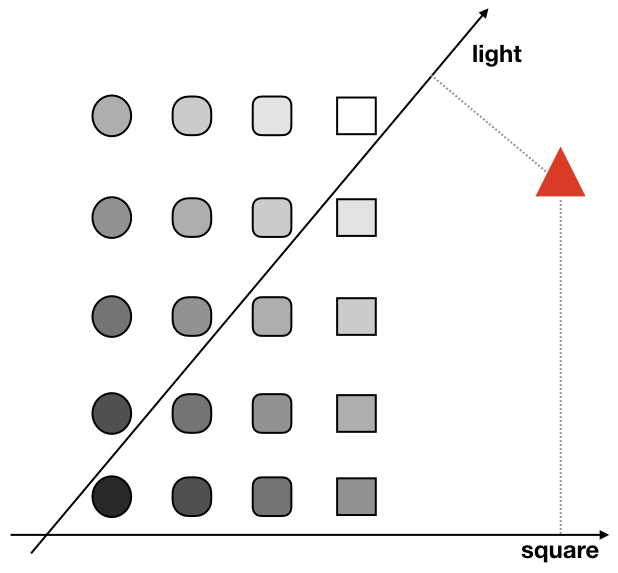
\includegraphics[width=180pt]{images/shapes}
	\caption{Toy example showing the effect of outliers in a two-dimensional embedding of geometric shapes.}
	\label{fig:toyExample}
\end{figure}

Ideally, representations would be learned with knowledge of feature-directions. For example, the method to learn a representation of the toy domain would know that it should model the features "square" and "light" rather than a similarity objective, so that this triangle would end up closer to the bottom-left corner. However, as we cannot a-priori determine the features the space must be learned from, it is difficult to learn a representation in this way. This Chapter instead introduces an unsupervised method that given a representation and its associated feature-directions, we can obtain a  vector space and associated feature-directions where the quality of the feature-directions is prioritized over the existing structure. The intention of this method is to resolve issues like those described in the previous two paragraphs.

To introduce the idea behind the method, we start with the assumption that each feature-direction has one feature-word, which describes the feature: if the feature-ranking of a document on a feature-direction is faithful to the bag-of-words score for the feature-word in the document, then the feature-ranking is good. To give an example of why this assumption is useful, in the IMDB movies domain \ref{datasets:movies} Multi-Dimensional Scaling (MDS) spaces there is the case of an Indian Bollywood movie that is very unlike other movies, as its reviews only use language specific to Bollywood films and the amount of reviews it has is low overall. This movie occupies a top-ranking position in a variety of feature-directions,  as a consequence of it being very dissimilar to other movies. The fine-tuning process solves this problem by attempting to match its  ranking in the vector space that is very high, to its bag-of-words value, which is zero. This results in this obscure outlier movie being moved down drastically in the rankings. 

To give some real examples, in Table \ref{tabTopRanked}, names of documents are shown ranked on feature directions in the domain of place-types (See Section \ref{datasets:placetypes}). In these examples, for the cluster-feature $\{\textit{steep},\textit{climb},\textit{slope}\}$, the top ranked document \textit{mountain} is clearly relevant. However, the next two documents --- \textit{landscape} and \textit{national park} --- are not directly related to this feature. Intuitively, they are ranked highly because of their similarity to \textit{mountain} in the vector space. Similarly, for the second feature, \textit{building} is ranked highly because of its similarity to \textit{skyscraper}, despite intuitively not having this feature. Finally, \textit{fence} received a high rank for several features,  mostly because it is an outlier in the space. 


\begin{table*}[t]
	
	\centering
	\setlength{\tabcolsep}{8pt}
	\renewcommand{\arraystretch}{1.2}
	\footnotesize
	\begin{tabularx}{\textwidth}{l l l}
		\toprule
		\textbf{Feature direction} & Highest ranking objects & Highest fine-tuned ranking objects\\
		\midrule              
		\{steep, climb, slope\}                   & mountain, landscape, national park & ski slope, steep slope, slope                                     \\
		\{illuminated, illumination, skyscraper\} & building, city, skyscraper         & tall building, office building, large building                    \\
		\{play, kid, kids\}                       & school, field, fence               & college classroom, classroom, school                              \\
		\{spooky, creepy, scary\}          & hallway, fence, building             & hospital room, hospital ward, patient room                  \\
		\{amazing, dream, awesome\}                   & fence, building, beach    & hotel pool, resort, beach resort \\
		\{pavement, streetlight, streets\}        & sidewalk, fence, building          & overpass road, overpass, road junction                            \\
		\{dead, hole, death\}                     & fence, steps, park                 & grave, cemetery, graveyard                                        \\
		\{spire, belltower, towers\}              & building, arch, house              & bell tower, arch, religious site                                  \\
		\{stones, moss, worldheritage\}           & landscape, fence, steps            & ancient site, ancient wall, tomb                                  \\
		\{mosaic, tile, bronze\}                  & building, city, steps              & cathedral, church, religious site     \\
		\bottomrule
	\end{tabularx}
	
	\caption{Comparing the highest ranking place-type objects in the original and fine-tuned space. \label{tabTopRanked}}
\end{table*}


Generally, the method that fine-tunes vector spaces and their associated feature-directions is as follows: First, a vector space is learned from bag-of-words representations of the considered documents, using a standard similarity-centric method or neural network. Next, the method from Chapter \ref{Chapter3} is used to  obtain feature-directions and their associated words from a vector space. Then, following our assumption outlined in the previous paragraph,  documents are ranked on the feature-direction's associated words using the bag-of-words. Finally, this ranking is used to fine-tune the vector space and feature-directions so that the resulting feature-rankings are more faithful to the ranking on the bag-of-words.

% Why does it work? What does it mean?

%This Chapter introduces a post-processing method on vector-spaces to obtain better feature-directions. First, the method described in Chapter \ref{Chapter3} is used to obtain  cluster-directions in a vector space. Then, we obtain a target-ranking  then the  feature-rankings of these directions are improved by shifting them closer to a ranking induced from PPMI scores. 


%In Chapter \ref{Chapter5}  feature directions in a variety of neural network architectures, and how these directions can be used to explain how these networks function was shown. In the case of stacked auto-encoders, however, we noticed that each layer became less and less interpretable.  Even in the case of feedforward networks, which generally remained more interpretable than stacked autoencoders, we noticed a clear drop in Kappa scores. The question we study in this chapter is whether it is possible to take a vector space which is less interpretable than we would like, and manipulate it so it models feature directions in a better way. The intuitive idea is to look at the features which are best represented in the initial vector space, and to fine-tune the representations so they capture these features in a more faithful way. Another way of looking at this is that our proposed method prioritises the interpretable features that are captured by a given vector space, possibly at the expense of other, less interpretable features.

%One way to apply this method is to a representation produced by an auto-encoder, ensuring that it retains key features in the representation while also reducing its size. % Talk about how it doesn't work?
 %Another way of applying this method is to the vector spaces and feature-directions found in Chapter \ref{Chapter3}. These vector space representations were learned with a similarity-centred objective, i.e.\ the main consideration when learning these representations is that similar documents should be represented as similar vectors. An important observation is that such spaces may not actually be optimal for modelling feature directions. 




%For example, \cite{Murphy} found that PCA dimensions did not typically make sense, and FRAGE \cite{Gong2018} achieved state-of-the-art results by removing the bias that a representation has for frequent words. If these biases exist, and the structure is influenced by the similarity such that it does not prioritize a directional structure, then it is unlikely to achieve good results with the method from Chapter 3.

%The aim of this Chapter is to focus the spatial representation on having good directions. This can be understood to be sacrificing similarity information in exchange for direction information. Using the method from the previous chapter,  semantically important feature-directions in a considered domain are determined. Then, from these directions the semantic space and the associated feature directions are fine-tuned to  better rank documents. 



  



This Chapter is a follow-up of the previous two Chapters, where previously feature-directions are identified in a variety of vector-spaces, and their potential applications are discussed, this Chapter focuses on improving the quality of these feature-directions to achieve better results. This Chapter continues with explaining the method to fine-tune a vector space and its associated feature directions using a bag-of-words in detail. Afterwards, we show  quantitative results to see how the fine-tuning affects simple interpretable classifiers (as in Chapter \ref{Chapter3}). Finally, we end with a conclusion for potential future work.


%We evaluate our method using one and three depth decision trees. For trees with a single node, we argue that improving the classification score of natural domain tasks, e.g. classifying the genre of movies by their reviews, is good evidence that the dimension used to classify the objective contains relevant domain knowledge and is self contained. We find that our fine-tuned representation improves the F1 score of depth one and depth three trees, sometimes substantially, and beats our baseline. Additionallly, we find that  often the single depth trees perform well for each class, sometimes even exceeding the depth three trees. In diagram 1, we give an example of a three depth decision tree from a domain of movie reviews, used to classify the 'Horror' genre. % Just an example



%We find that our fine-tuned representation consistently improves depth one and depth three decision trees, sometimes substantially. Additionally, we find that the single depth trees perform well for many classes, often performing on par with, or even better than larger decision trees. \todo{In diagram 1, we give an example of a three depth decision tree from a domain of movie reviews, used to classify the 'Horror' genre}. 

%The remainder of the paper is structured as follows. After presenting related work in the next section, Section \ref{LearningInterpretableDirections} explains how interpretable directions are identified from the initial vector space, while Section \ref{secFinetuning} introduces our proposed fine-tuning method. Finally, in Section \ref{secExperiments} we present our experimental results, showing that decision trees learned from the fine-tuned rankings perform we
%In our work, we aim to obtain a fine-grained, conceptually sound interpretable representation in an entirely unsupervised way. We follow previous work, where authors \cite{Derrac2015} used an unsupervised method to obtain fine-grained interpretable rankings of entities from a vector space wherein entities correspond to points, and concepts to regions e.g. in a vector space learned from wine tasting notes, a ranking of wines based on how many $'tannins'$ they have. They did this by finding highly separable terms e.g. in a space learned from movie reviews, $'scary'$, $'funny'$,  $'romantic'$, and a corresponding direction for each of these terms. These directions were then clustered together  $'scary'$, $'gory'$, $'terrifying'$ using a simple K-means algorithm. Finally, a ranking was induced for each entity on each cluster (e.g. a ranking of how $'scary'$ each movie is), and used as input to an interpretable classifier, e.g. a Decision Tree classifying the genre of a movie. See Fig 1.

%\begin{figure*}
%\includegraphics[scale=0.3]{horror-ndcg-finetune.png}
%\centering
%\caption{A Decision Tree obtained using our process that classifies if a movie is in the "Horror" genre.}
%\end{figure*}

%Previously, authors  \cite{Steven} used an unsupervised method to represent semantic relationships learned in a vector space in the form of fine-grained interpretable rankings of \textit{entities}, e.g. in a vector space learned from \textit{wine} tasting notes, a ranking of \textit{wines} based on how many $'tannins'$ they have. In their work, they learned a vector space wherein entities are points in the space, and concepts are regions. Then, they obtained a hyperplane that separates entities for each term, scored by separability. Highly separable terms we can understand correspond to natural concepts (e.g. in a space learned from movie reviews, $'scary'$, $'funny'$,  $'romantic'$). From these hyperplanes, we can obtain their orthogonal directions, and then induce a ranking of entities on this direction by obtaining the dot product of the entity points on the direction vectors (e.g. a ranking of how $'scary'$ each movie is). These directions can be clustered together by similarity e.g. $'scary'$, $'gory'$, $'terrifying'$, and used as input to an interpretable classifier.

%In our work, we learn fine-grained interpretable features that better represent natural concepts in the domain, by describing the representation of the relationship between entities more accurately in the domain, and validate that our model performs greater than previous methods by learning shallow decision trees, see figure 1.

%What are other approaches? What is our approach? Why is it important?

%What previous  work are we building on? Why is this information important? How does it fit into our work? How does it separate from our work?

%Previously, authors  \cite{Steven} used an unsupervised method to represent semantic relationships learned in a vector space in the form of fine-grained interpretable rankings of \textit{entities}, e.g. in a vector space learned from \textit{wine} tasting notes, a ranking of \textit{wines} based on how many $'tannins'$ they have. In their work, they learned a vector space wherein entities are points in the space, and concepts are regions. Then, they obtained a hyperplane that separates entities for each term, scored by separability. Highly separable terms we can understand correspond to natural concepts (e.g. in a space learned from movie reviews, $'scary'$, $'funny'$,  $'romantic'$). From these hyperplanes, we can obtain their orthogonal directions, and then induce a ranking of entities on this direction by obtaining the dot product of the entity points on the direction vectors (e.g. a ranking of how $'scary'$ each movie is). These directions can be clustered together by similarity e.g. $'scary'$, $'gory'$, $'terrifying'$, and used as input to an interpretable classifier.

%Granular rankings lead to more fine-grained control, meaning that sensitive issues can be resolved granularly.

%What is our work? What is the novelty of the contribution? How does it affect the results? In what ways is it better? 

% So our work is about learning a more accurate representation following Steven's work

%We introduce an unsupervised method to improve the accuracy of salient directions, by using them as weights in a neural network, that trains these directions to be closer to their bag-of-words representation, while maintaining fidelity to the original rankings. To test these rankings, we then use them as the input to a low-depth decision tree, which we use as a quantitative measure to show that our features are more accurate and interpretable than both a Latent Dirchlet Allocation (LDA) baseline and previous work. We evaluate our work in three different domains, movie reviews, flickr tags describing place-types, and the 20 newsgroups dataset.

%The rest of this paper is organized as follows. Section 2 describes related literature, Section 3 describes previous work in more detail that we use to obtain directions and rankings, Section 4 describes our work, Section 5 details our experiments and we conclude the work in Section 6. 

%
%\section{Related Work}

% Other approaches offer different ways of attacking the same problem
% Topic models give statistical models, additionally leveraging labelled data or relaxing/adding constraints

%-------------
% Interpretability, other approaches to interpretability
% Our approach to interpretability, specifically text representations ala: PCA, Sparse PCA,
% LDA, 
% NMF,
% Word vectors, sparsity applications
% Final statement clarifying differences and setting up the description of our work
%-------------

%One method in particular has achieved global explanations \cite{Lakkaraju2017}, by obtaining decision sets that approximate an existing model. 

% Something about linear models?

% Topic models




%The most commonly used representations for text classification are bag-of-words representations, topic models, and vector space models. Bag-of-words representations are often too simplistic and sparse to perform well, unless a bag of word vectors is used, or tailored to the domain in some way. Topic models and vector space models are two alternative approaches for generating low-dimensional document representations.

%\textbf{Topic models.} 
%Similarly, our feature directions are also labelled with the most closely associated words. 
%However, while LDA only uses bag-of-words (BoW) representations, our focus is specifically on identifying and improving features that are modelled as directions in semantic spaces. 

%\todo{Say something about the problem of assigning (single) labels to topics; lots of people have looked at doing something more sophisticated then simply describing topics using the top few terms, and these approaches are also relevant to this paper as we might in principle use similar methods to label our directions.}
%where documents are represented by a distribution of topics, and each topic is a distribution over words \cite{Blei2003}.  By simply taking the words with the top probability for a topic, we can easily obtain coherent topics. 
%removed a bunch of stuff about document classification
%LDA has been extended by many approaches, e.g.\ aiming to avoid the need to manually specify the number of topics \cite{teh2005sharing}, modelling correlations between topics \cite{Blei2006}, or by incorporating meta-data such as authors \cite{rosen2004author} or time stamps \cite{wang2006topics}.

%Topic models and our work, on the surface, produce similar results, as both representations result in distinct dimensions or topics, with documents having an associated numerical value for these topics. However, our method differs in the way these dimensions are obtained, in particular as we rely on the directions in a vector space rather than the raw bag-of-words, our method has the applicability to make use of specialist vector space representations tailored to an objective, e.g. a hidden layer output representation obtained from an Long-Short Term Memory network trained to classify sentiment, with very little adjustment.
%Broadly speaking, in the context of document classification, the main advantage of topic models is that their topics tend to be well separated and easy to make sense of, while vector space models tend to be more flexible in the kind of meta-data that can be exploited. The approach we propose in this paper aims to combine the best of both worlds, by providing a way to derive representations with distinct labelled dimensions from vector space models.


%\textbf{Vector space models} typically use a form of matrix factorization to obtain low-dimensional document representations. By far the most common approach is to use Singular Value Decomposition \cite{ASI:ASI1}, although other approaches have been advocated as well. 
%One approach which is of particular interest is non-negative matrix factorization (NMF), in which dimensions correspond to a non-negative combination of words. This is assumed to help interpretability as it means that dimensions can essentially be viewed as topics (i.e.\ they also correspond to weighted sets of words). 
%\todo{Have you found any references where NMF is used for document representation (we are not so much concerned with word vectors in this paper ...)?} 
%Instead of matrix factorization, another possible strategy is to use a neural network or least squares optimization approach. This is commonly used for generating word embeddings \cite{DBLP:conf/nips/MikolovSCCD13,glove2014}, but can similarly be used to learn representations of text documents \cite{DBLP:journals/corr/DaiOL15,van2016learning,DBLP:conf/sigir/JameelBS17}. Such approaches have the advantage that various forms of domain-specific structured knowledge can easily be taken into account. Some authors have also proposed hybrid models, which combine topic models and vector space models. For example, the Gaussian LDA model represents topics as multivariate Gaussian distributions over a word embedding \cite{DBLP:conf/acl/DasZD15}. Beyond document representation, topic models have also been used to improve word embedding models, by learning a different vector for each topic-word combination \cite{DBLP:conf/aaai/LiuLCS15}.

%\smallskip
%\noindent \textbf{Fine-tuning embeddings.} Several authors have looked at approaches for adapting word embeddings. One possible strategy is to change how the embedding is learned in the first place. For example, some approaches have been proposed to learn word embeddings that are better suited at capturing sentiment \cite{tang2016sentiment}, or to learn embeddings that are optimized for relation extraction \cite{DBLP:conf/conll/HashimotoSMT15}.
%Other approaches, however, start with a pre-trained embedding, which is then modified in a particular way. For example, in \cite{faruqui2015retrofitting} a method is proposed to bring the vectors of semantically related words, as specified in a given lexicon, closer together. Similarly \cite{yu2017refining} propose a method for refining word vectors to improve how well they model sentiment. In \cite{labutov2013re} a method is discussed to adapt word embeddings based on a given supervised classification task.

%Another way of approaching interpretability is non-negative matrix factorization. NMF has been applied to word vectors \cite{Murphy}, obtaining word-representations (NNSE) that are both accurate and interpretable. Fyshe \cite{Fyshe} also obtained interpretable and accurate representations by adding an additional compositionality constraint to NNSE in order to represent phrasal semantics. 

%Another way of representing text is to learn vectors for each word, by learning distributions from their context. This approach, popularized by GloVe and word2vec have achieved great results in real world applications like entity recognition, semantic role labelling and syntactic parsing \cite{Chen2014,Chen2014b,Guo2014}.    The idea of learning a distribution based on context has also been applied to sentences \cite{Liu2017}, paragraphs and documents \cite{Le2014} with to obtain document representations that perform well at classification tasks. However, these Paragraph Vectors have much less interpretable dimensions \cite{Le2014}.



% Paragraph on word vectors
%Distributional representations of words learned using contextual information have achieved state-of-the-art for many tasks. 




%-------------
% LDA
% LDA for document classification
% Unsupervised LDA approaches
% Supervised (relevant?) LDA approaches
%-------------

% An effective state-of-the-art representation learned using neural networks are word vectors
% Word vectors are effective at representing important concepts, and show high separability
% Further, they've been applied to documents effectively, and show high performance there too.
% However, these standard representations are not very interpretable.
% That's why some authors have applied sparsity and non-negativity constraints to a matrix factorization process
% For documents too
% Mostly, that's how word vectors have been used to obtain an interpretable representation, and like ours, they aim to be both accurate and interpreatble. However, we do not leverage contextual inforamtion in our learning process, instead relying on the raw meaning of each word to improve a set of rankings.

%Recently, a "bag-of-concepts" was also introduced, where word-vectors were clustered and averaged to form a concept. These are particularly relevant to our work, as we also obtain rich representations of words in the form of rankings and cluster them together to form a salient concept. 
%NOTE: This ^ seems like a common approach labelled "bag-of-clusters" for supposed novelty
%Further, there have been representations that combine the power of word vectors and topic models together. \cite{X} and \cite{bibid} did XXXX YYYY, and \cite{bibid} obtained an interpretable document representation that used both.


%-------------
% NMF
% Variations of NMF
% Word vectors, Variations on word vectors for sentences/paragraphs
% Sparse word vectors
% Sparse document vectors
%-------------

%An alternative was introduced by \cite{IDK} as a "bag-of-concepts", where word vectors are clustered together and averaged.   ### This work seemed to be aready done essentially ### Our work is similar in the sense that we cluster together semantic representations of words, but we instead represent words as concepts and a group of words as a direction and associated ranking. Some recent approaches have combined the use of both topic-models and word-vectors, attempting to leverage contextual information to learn better topics or words in a "two-step" process, or combine both procedures together into a single model. Other works that use structural information as part of their learning process to learn an interpretable representation are , who used the structural information of sentences in combination with an attention mechanism to produce document representations with interpretable intermediate structures. 





%have been argued to be less interpretable, and instead a "bag-of-concepts" - has been used, clustering multiple word-embeddings together into concepts, and then using those now interpretable features to classify documents \cite{Kim2017}. We can understand the previous work \cite{Steven}   to be most similar to clustering multiple word-embeddings together, as they also obtain interpretable features from a cluster of properties. However, our work obtains interpretable features from an existing representation, rather than learning a more accurate or interpretable representation. 

%Supervised approaches use labelled data to make a models probabilities more suitable for classification, for example \cite{VanLinh2017} have used supervised data to train a topic model for document classification. %Stuff about unsupervised methods.

%Recently, 'Representation Learning' \cite{Bengio2012} with neural networks have learned text representations that are 'disentangled', meaning that natural domain concepts are well separated in the space.



%Other approaches have looked at combining the structural information of the text into the representation to make it more interpretable.

%However it seems to have potential for producing the kind of 'conceptual space' that the original work derived their inspiration for a vector space to derive semantic relationships from \cite{Bechberger}. 





%Another approach to obtaining a better interpretable classifier is to learn a linear model using an existing black-box model. These approaches are limited to the black-box model they are learning from, and are sometimes reliant on a certain kind of neural network or feature representation. 

%The importance of the salient features of the domain being distinguished from each other has been recognized across many different domains. The most common way of determining these features is understanding what the dimensions of vectors mean, in the context of word vectors this has been achieved by obtaining high-scoring words for the particular dimension and a high-scoring word from another dimension. Being able to judge the difference essentially tests how interpretable the dimension is.

%Our method does not rely on the model and is not totally independent from it. We essentially rely on a good representation that has disentangled the natural features of the domain, and attempt to achieve that by tuning the representation towards a natural classification task. Further, we are not particularly interested in an explanation of the neural network model, rather we want to obtain interpretable features that correspond to natural domain concepts so we can build an interpretable classifier from these features. 


% Might be valuable, but from 2013...
%The quality of a vector space representation has been described as the extent to which semantic concepts are well separated in the space \cite{Bengio2013}, and the ability to obtain these 'disentangled' spaces using neural networks has been widely explored. 


%Typically, rankings of entities are based on features from a knowledge base \cite{Schuhmacher2015}. However, we are interested in improving rankings derived from directions in our space. To do so, we use a novel kind of neural network that outputs the rankings of the clusters and trains them to be closer to the original PPMI values. We can consider this to be fine-tuning the space to become more interpretable. Other works have focused on guiding the hidden layer representation of the network to obtain better rules,  Similar to the concept of improving the space dependent on important features \cite{Chen2016} learns a representation by maximizing the mutual information between a small subset of latent variables that are relevant to a classification task. This method is a form of representation learning, where the representation learned has disentangled the space such that the natural clusters in the data form. However, the variables chosen to be tuned for this method were hand-selected, while the features we tune are obtained in an unsupervised way. Not only that, but we are not necessarily interested in disentangling the space, rather we are interested in a space that can create better rankings so we can use them as the input to an interpretable classifier. 



%Recently, methods to obtain explanations from neural networks by perturbing the inputs and observing the changes to the outputs have risen to prominence as a method to interpret classification decisions. LIME \cite{Ribeiro2016}  obtains a method that can explain the decision of any classifier.  This approach can build trust for the prediction of any classifier, but does not explain the building blocks that lead to the solution. In contrast, our approach makes explicit the semantic relationships that it builds on for classification, and describes meaningful rankings of entities according to these relationships. Some methods, similar to ours, rely on a text-based neural network to function. In \cite{Lei2016}, pieces of input text are extracted to justify predictions, while in \cite{Li2016} the effects of erasure are used to analyse and interpret decisions. However, these methods often do not give the whole picture.  By producing an interpretable classifier, both the prediction is explained and the knowledge of how the classifier has understood the problem is explained. Even though hard to interpret models generally have higher accuracy, it can be difficulty to improve the accuracy of the model based on an explanation of the output alone. In contrast, all information used by the classifier, including its decisions in the trained model, can be both understood and controlled by the user. Further, an interpretable classifier derived from the hidden layer of a network that is classifying the same objective can serve as an explanation of the main concepts learned by the network, with the additional benefit of being able to classify new information in an interpretable way.

%Similar to obtaining interpretable features, obtaining intepretable rules from neural networks has also been previously explored. The existing neural network rule extraction algorithms can be categorized as either decompositional, pedagogical or eclectic \cite{Andrews1995a}. Decompositional approaches derive rules by analysing the units of the network, while pedagogical approaches treat the network as a black box, and examine the global relationships between inputs and outputs. Eclectic approaches use elements of both decompositional and pedagogical approaches. The algorithm in \cite{Kim2000} is a decompositional approach that applies to a neural network with two hidden layers. It uses hyperplanes based on the weight parameters of the first layer, and then combines them into a decision tree. Our method is similar in that it also uses hyperplanes to obtain property directions, but we provide an unsupervised and more large-scale approach for text-classification, that results in interpretable rankings. NeuroLinear \cite{Setiono1997c} is a decompositional approach applied to a neural network with a single hidden layer that discretizes hidden unit activation values and uses a hyperplane rule to represent the relationship between the discretized values and the first layer's weights. HYPINV \cite{Saad2007b} is a pedagogical approach that calculates changes to the input of the network to find hyperplane rules that explain how the network functions.



%\section{Identifying Feature Directions}\label{LearningInterpretableDirections}


%We assume that a domain-specific semantic space is given, and that for each of the objects which are modelled in this space, we also have a BoW representation. 
%Our overall aim is to find directions in the semantic space that model salient features of the considered domain. For example, given a semantic space of movies, we would like to find a direction that models the extent to which each movie is scary, among others. Such a direction would then allow us to rank movies from the least scary to the most scary. We will refer to such directions as \emph{feature directions}. Formally, each feature direction will be modelled as a vector $v_f$. However, we refer to \emph{directions} rather than \emph{vectors} to emphasize their intended ordinal meaning: feature directions are aimed at ranking objects rather than e.g.\ measuring degrees of similarity. In particular, if $o$ is the vector representation of a given object then we can think of the dot product $v_f \cdot o$ as the value of object $o$ for feature $f$, and in particular, we take $v_f \cdot o_1 < v_f \cdot o_2$ to mean that $o_2$ has the feature $f$ to a greater extent than $o_1$.

%To identify feature directions, we use a variant of the unsupervised method proposed in \cite{derracAIJ}, which we explain in this section. In Section \ref{secFinetuning}, we will then introduce our approach for fine-tuning the semantic space and associated feature directions. 


%\smallskip
%\noindent \textbf{Step 1: Generating candidate feature directions.} Each feature will be associated with a cluster of words, which we can regard as a description of the intuitive meaning of that feature. Since we assume no \emph{a priori} information about which words might describe features that can be modelled as directions in the vector space, the method initially considers all nouns and adjectives that are sufficiently frequent in the BoW representations of the objects as candidate feature labels. Then, for each considered word $w$, a logistic regression classifier is trained to find a hyperplane $H_w$ in the semantic space that separates objects which contain $w$ in their BoW representation from those that do not. The vector $v_w$ perpendicular to this hyperplane is then taken as the direction that models the word $w$. 
%Let $o_1$ and $o_2$ be the vector representations of two objects. If $v_w$ models the word $w$ well, we would expect that $v_w \cdot o_1 < v_2 \cdot o_2$ if the word $w$ is more strongly related to $o_2$ than to $o_1$. For example, in a space of movies, if $w$ is the word `scary', then we would expect $v_w$ to rank the movies according to how scary they are. 

%\smallskip
%\noindent \textbf{Step 2: Filtering candidate feature directions.} To determine whether the word $w$ is likely to describe an important feature for the considered domain, we then evaluate the quality of the candidate feature direction $v_w$. For example, we can use the classification accuracy to evaluate the quality in terms of the corresponding logistic regression classifier: if this classifier is sufficiently accurate, it must mean that whether word $w$ relates to object $o$ (i.e.\ whether it is used in the description of $o$) is important enough to affect the semantic space representation of $o$. In such a case, it seems reasonable to assume that $w$ describes an important feature for the given domain. 

%One problem with accuracy as a scoring function is that these classification problems are often very imbalanced. In particular, for very rare words, a high accuracy might not necessarily imply that the corresponding direction is accurate. For this reason, \newcite{derracAIJ} proposed to use Cohen's Kappa score instead. In our experiments, however, we found that accuracy sometimes yields better results, so rather than fix the scoring function, we keep this as a hyperparameter of the model that can be tuned. 

%In addition to accuracy and Kappa, we also consider Normalized Discounted Cumulative Gain (NDCG). 
%This is a standard metric in information retrieval which evaluates the quality of a ranking w.r.t.\ some given relevance scores \cite{jarvelin2002cumulated}.  In our case, the rankings of the objects $o$ are those induced by the dot products $v_w \cdot o$ and the relevance scores are determined by the Pointwise Positive Mutual Information (PPMI) score $\textit{ppmi}(w,o)$, of the word $w$ in the BoW representation of object $o$ where
%$\textit{ppmi}(w,o) = \max \big(0, \log\big(\frac{p_{wo}}{p_{w*} \cdotp p_{*o}}\big)\big)$, and
%\begin{align*}
%p_{wo} &= \frac{n(w, o)}{\sum_{w'} \sum_{o'} n(w', o')}
%\end{align*}
%where $n(w,o)$ is the number of occurrences of $w$ in the BoW representation of object $o$, $p_{w*} = \sum_{o'} p_{wo'}$ and $p_{*o} = \sum_{w'} p_{w'o}$.
%In principle, we may expect that accuracy and Kappa are best suited for binary features, as they rely on a hard separation in the space between objects that have the word in their BoW representation and those that do not, while NDCG should be better suited for gradual features. In practice, however, we could not find such a clear pattern in the differences between the words chosen by these metrics despite often finding different words.




%While the Kappa metric was found to perform well, one drawback is that it does not actually evaluate the ranking of the documents induced by $v_w$. To address this, in this paper we will also consider the normalized discounted cumulative gain (NDCG) metric \cite{jarvelin2002cumulated} and, following good results, the accuracy metric. 
% ???? SHOULD WE TALK ABOUT NDCG? NOT SURE IF RESULTS ARE GOOD ????

% [REMOVED, DIDNT TEST WITH PRIMAL DIRS] We also carried out some initial experiments with other ranking evaluation metrics, such as Spearman's $\rho$, but found NDCG to give the most promising results. %\todo{....} Table \ref{tabKappaNDCG} shows the words with the highest Kappa score and the words with the highest NDCG score in a space of movies. As can be observed, the Kappa score gives a higher prominence to binary properties \todo{add examples}, whereas the NDCG score leads us to select more gradual properties \todo{add examples}.



%\smallskip
%\noindent \textbf{Step 3: clustering candidate feature directions.}
%As the final step, we cluster the best-scoring candidate feature directions $v_w$. Each of these clusters will then define one of the feature directions to be used in applications. The purpose of this clustering step is three-fold: it will ensure that the feature directions are sufficiently different (e.g.\ in a space of movies there is little point in having \emph{funny} and \emph{hilarious} as separate features), it will make the features easier to interpret (as a cluster of terms is more descriptive than an individual term), and it will alleviate sparsity issues when we want to relate features with the BoW representation, which will play an important role for the fine-tuning method described in the next section.

%As input to the clustering algorithm, we consider the $N$ best-scoring candidate feature directions $v_w$, where $N$ is a hyperparameter. To cluster these $N$ vectors, we have followed the approach proposed in \cite{derracAIJ}, which we found to perform slightly better than $K$-means. The main idea underlying their approach is to select the cluster centers such that (i) they are among the top-scoring candidate feature directions, and (ii) are as close to being orthogonal to each other as possible. We refer to \cite{derracAIJ} for more details. 
%To cluster these $N$ vectors, we have used a version of} the standard $K$-means clustering algorithm for this purpose, \blue{where cosine similarity is used instead of Euclidean distance}.  
%The output of this step is a set of clusters $C_1,...,C_K$, where we will identify each cluster $C_j$ with a set of words.
%We will furthermore write $v_{C_j}$ to denote the centroid of the directions corresponding to the words in the cluster $C_j$, which can be computed as $v_{C_j}= \frac{1}{|C_j|} \sum_{w_l\in C_j} v_l$ provided that the vectors $v_w$ are all normalized. These centroids $v_{C_1},...,v_{C_k}$ are the feature directions that are identified by our method. 

%Table \ref{tabKappaNDCG} displays some examples of clusters that have been obtained for three of the datasets that will be used in the experiments, modelling respectively movies, place-types and newsgroup postings. For each dataset, we used the scoring function that led to the best performance on development data(see Section \ref{secExperiments}). Only the first four words whose direction is closest to the centroid $v_C$ are shown.

%Selected from using the top-scoring depth-3 tree parameter variations on development data. IMDB Sentiment omitted as it is similar to movie reviews. We find that different scoring-types find different kinds of properties. In this case, we can see that NDCG in particular has found quite specific, almost somewhat niche clusters that correspond to specific types of movies, while the kappa-scored terms are more general and easy to grasp.

%The clusters are assumed to correspond to the most salient properties from the domain of interest. In \cite{derracAIJ} these properties were used to generate commonsense ``a fortiori'' rules of the form ``if $X$ is a Thriller movie and $Y$ is \emph{more scary} than $X$, then $Y$ is a Thriller movie as well'', where `Thriller movie' corresponds to the class that we want to predict and `scary' in this case is one of the properties that was identified from the vector space. In this paper, we will evaluate the usefulness of such properties as features for learning small and interpretable decision trees. 




%When obtaining properties, we only consider terms that have occurred in at least 100 entities for the movies, 50 entities for the place-types and 30 entities for the newsgroups. Additionally, we did not include terms that were included in more than $|E| - 10$ entities. These thresholds were chosen such that the amount of terms were roughly equivalent to the datasets chosen in the previous work, resulting in 6335 terms for the newsgroups, 27385 terms for the movies, and 21836 terms for the place-types. 

% NOTE: These are copy pasted from past workshop paper. Probably need some changes


%\paragraph{Identifying directions for frequent terms.} To discover terms that correspond to interpretable properties in the MDS space, the nouns and adjectives that occur in sufficiently many reviews are converted to a binary bag-of-words representation and used as input to a linear Support Vector Machine (SVM)\footnote{\url{http://scikit-learn.org/stable/modules/generated/sklearn.svm.LinearSVC.html}}. The SVM is trained to find the hyperplane that best separates the entities that contain the term at least once in their associated textual description. To accommodate class imbalance, we increase the cost of positive instances such that their weight is inversely proportional to how many times the term has occurred. To assess the quality of the hyperplane found by the SVM, we use Cohen's Kappa score \cite{cohen1960}\footnote{\url{http://scikit-learn.org/stable/modules/generated/sklearn.metrics.cohen_kappa_score.html}} which evaluates how well the hyperplane separates positive/negative instances while taking class imbalance into account. We consider terms with a high Kappa score to be labels of properties that are modelled well by the MDS space. The direction corresponding to a given term/property is given by the vector perpendicular to the associated hyperplane. This vector in turn allows us to determine a ranking of the entities, according to how much they have the  property being modelled. This ranking is obtained by determining the orthogonal projection of each entity on an oriented line with that direction. It is easy to see that if $v$ is the vector modelling a given property, then entity $e_1$ is ranked before entity $e_2$ iff $e_1 \cdot v < e_2 \cdot v$. Another way to look at this is that entities are ranked according to their signed distance to the hyperplane.

%\paragraph{Improving the scoring method.} In the method described by \cite{Derrac2015}, the quality of a property was determined by how well entities that have a property were separated in a space, measured using the Kappa score. We can expect this method to find more "binary" properties, e.g. a film will either have gore, or not have any gore at all. In-order to find other kinds of properties, we can instead use a metric that measures how well a direction $d_{t}$ is modelled in the space directly. To do this, we use Normalized Discounted Cumulative Gain (nDCG) \cite{Words2002}\footnote{\url{https://gist.github.com/mblondel/7337391}} to measure the quality of the ranking induced from the direction. This method takes relevance scores for each entity, and a ranking, and outputs an nDCG score for how effective the ranking is at matching those relevance scores, with a greater weight for those entities that are higher up in the ranking. As the PPMI scores are sparse, this means that many of the entities that are relevant but have a PPMI score of 0 do not make much of an impact on the overall score, essentially allowing us to compare the rankings of those entities that do have an associated PPMI score more effectively than if we had weighted each position equally. The rankings $r$ we evaluate are the ones induced from the direction $d_{t}$, which we obtain from the dot product of the entity vector on the property direction $rank(e, d_{t})$, and we use the PPMI values as the relevance scores $ppmi(e, t)$, under the assumption that they correspond to a good baseline for what we consider to be important for an entity. 
% Taken directly from the journal paper
%\begin{align*}
%\text{DCG}_{r}^{t} &= \sum_{i=1}^{p}\frac{\textit{ppmi}_{i}^{t}}{log_{2}(i + 1)} \\
%\text{IDCG}_{r}^{t} &= \sum^{|\textit{entities}|}_{i=1} \frac{2^{\textit{ppmi}_{i}^{t}}-1}{log_{2}(i + 1)} \\
%\text{nDCG}_{r}^{t} &= \frac{\text{DCG}_{r}^{t}}{\text{IDCG}_{r}^{t}}
%\end{align*}  

%To define nDCG, we can first define Discounted Cumulative Gain (DCG), where $p$ is equal to a position in the ranking of entities on a direction $d_{t}$, and $ppmi_{p_{i}}^{t}$ is equal to the PPMI score for a term at position $i$ in the ranking. Then, we can define the Ideal Discounted Cumulative Gain (IDCG), which is the best possible DCG for a position $p$, where $|entities|$ are the entities for the term ordered by their relevance up to position $p$. nDCG is then simply the DCG normalized by the iDCG.  %Below, we show the top 20 highest scoring properties that are not in the top 100 properties when using the other scoring method. As there are a few duplicates between both methods, this is simply to highlight the different kinds of properties each one obtains.


%By examining these properties, we can see that there are a few distinct kinds of properties. On the Kappa score side, there are specific aspects of technology, e.g. blu, meaning blu-ray, vhs, referring to older methods of storage, as well as transfer. These are markedly absent in NDCG, assumedly because they are so binary - a movie is either on vhs or not on vhs. On NDCG's side, we begin to see more informative properties. "prison", "musicals" "western" are all very useful for classifying the type of movie. However, NDCG also finds an interesting somewhat unique collection of propertioes "Branaghs" "astaire" and "crawford" are all names, relating to the movie industry in some way. 

% Deleted stuff by accident here.} These properties are informative, but often repetitive and are sometimes difficult to understand without additional context. In-order to obtain meaningful directions, we can cluster together salient properties to obtain a cluster of terms $c = \{t_{1},  ... , t_{n}\} $, that correspond to a single cluster direction. We first choose the number of clusters equal to the number of dimensions. To determine the cluster centers, we first select directions whose associated Kappa score is above some threshold $T^+$. We  use the highest scoring direction as the center of the first cluster and find the most dissimilar direction to the first cluster's direction to get the centre of the second cluster. Continuing in this way, we repeatedly select the direction which is most dissimilar to all previously selected clusters. By doing so, we obtain a collection of cluster centres that capture a wide variety of different properties from the space. We then associate each remaining direction to its most similar cluster centre. In this step, past work considered  directions whose associated Kappa score is at least $T^-$, where typically $T^-<T^+$. However,  Finally, we take the average of all directions in a cluster to be the overall direction for a cluster. The value of $T^+$ should be chosen as large as possible (given that the terms with the highest Kappa scores are those which are best represented in the space), while still ensuring that we can avoid choosing cluster centers which are too similar. 



%************************************************************************************************
\section{Fine-Tuning Vector Spaces And Their Associated Feature Directions}\label{secFinetuning}


%This is essentially re-organizing the space so that feature-directions are prioritized. However, it is important that what was learned in the space is not forgotten. This is why feature-rankings are trained to be more faithful to the PPMI ranking, not to exactly match it. 


%Standard dimensionality reduction methods such as singular value decomposition or Multi-Dimensional Scaling (MDS) aim to learn a vector space that preserves, as much as possible, the similarity structure between the considered text documents. However, for our purposes, the quality of the rankings induced by the interpretable directions is more important than the overall similarity structure. 

%For the property \todo{},  we find movies such as \todo{}, which are not actually related to this property. The underlying reason is that these movies are outliers in the considered collection. As a result, their vector representation will also be significantly different from the average, and thus they will tend to receive extreme positions in the rankings induced by the interpretable directions. \todo{Try to find examples (not necessarily from the movies space) of other types of issues with initial vector space that get resolved by the fine-tuning step. Maybe something with two documents that are very similar overall (and thus get a very similar vector representation), but differ in one of the properties, where because of their similarity, they initially get a similar rank, even for the property in which they differ.}

To improve the directions and address these problems, we propose a method for fine-tuning the semantic space representations and corresponding feature directions. First, it is explained how to obtain target rankings from PPMI scores. Then, the neural network that uses these target rankings to improve the vector space and its associated feature-directions is described. The main  idea is to use the BoW representations of the objects as a kind of weak supervision signal: if an object should be ranked highly for a given feature, we would expect the words describing that feature to appear frequently in its description.
%In particular, from the BoW representations, we first construct target rankings for each of the feature directions. 
To obtain the target rankings, for each feature $f$ we determine a total ordering $\preccurlyeq_f$ such that $o \preccurlyeq_f o'$ iff the feature $f$ is more prominent in the BoW represention of object $o'$ than in the BoW representation of $o$. We will refer to $\preccurlyeq_f$ as the \emph{target ranking} for feature $f$. If the feature directions are in perfect agreement with this target ranking, it would be the case that $o \preccurlyeq o'$ iff  $v_C \cdot o \leq v_C \cdot o'$. Since this will typically not be the case, we subsequently determine \emph{target values} for the dot products $v_C \cdot o$. These target values represent the minimal way in which the dot products need to be changed to ensure that they respect the target ranking.
%from the BoW representations, we first construct target rankings for each of the feature directions. 
%Using these target rankings, we then determine target values for these dot products, which respect the chosen target rankings but otherwise stay as close as possible to the initial values. 
Once these rankings have been obtained, we use a simple feedforward neural network to adapt the semantic space representations $o$ and feature directions $v_C$ to make the dot products $v_C \cdot o$ as close as possible to these target values. 

\subsection{Generating Target Rankings}\label{secTargetRankings} \raggedbottom 
Let $C_1,...,C_K$ be the clusters that were found using the method from Section \ref{ch3:LearningInterpretableDirections}. 
Each cluster $C_i$ typically corresponds to a set of semantically related words $\{w_1,...,w_n\}$, which describe some salient feature from the considered domain. 
From the BoW representations of the objects, we can now define a ranking that reflects how strongly each object is related to the words from this cluster. To this end, we represent each object as a bag of clusters (BoC) and then compute PPMI scores over this representation. In particular, for a cluster $C = \{w_1,...,w_m\}$, we define $n(C,o)=\sum_{i=1}^m n(w_i,o)$. In other words, $n(C,o)$ is the total number of occurrences of words from cluster $C$ in BoW representation of $o$. We then write $\textit{ppmi}(C,o)$ for the PPMI score corresponding to this BoC representation, which is evaluated in the same way as $\textit{ppmi}(C,o)$, but using the counts $n(C,o)$ rather than $n(w,o)$. The target ranking for cluster $C_i$ is then such that $o_1$ is ranked higher than $o_2$ iff $\textit{ppmi}(C_i,o_1) > \textit{ppmi}(C_i,o_2)$. By computing PPMI scores w.r.t.\ clusters of words, we alleviate problems with sparsity and synonymy, which in turn allows us to better estimate the intensity with which a given feature applies to the object. For instance, an object describing a violent movie might not actually mention the word `violent', but would likely mention at least some of the words from the same cluster (e.g.\ `bloody' `brutal' `violence' `gory'). Similarly, this approach allows us to avoid problems with ambiguous word usage; e.g.\ if a movie is said to contain `violent language', it will not be identified as violent if other words related to this feature are rarely mentioned.

%Our goal is to obtain an accurate set of rankings in an unsupervised way for salient directions in a vector space. In-order to do this, we introduce an unsupervised way to train our rankings to be more accurate. We begin by using the PPMI $ppmi(e, t)$ values, as they have detailed information about the relevance of a term to an entity. However, each cluster is composed of multiple terms $c = \{t_{1},  ... , t_{n}\} $. In-order to obtain a PPMI value for each cluster, we begin by summing together the frequency values $f$ of the terms $t$ in the cluster $ \vec{c_{t}}=\sum_{\mathrm{t}\in \mathrm{c}}\vec{f_{\mathrm{t}}}$. Once we've obtained these frequency values for each cluster, we obtain new PPMI values, using the frequencies of the clusters as the input. Where  $a(e, c)$ is equal to the sum of the times all terms in cluster $c$ have occurred in document $D_{e}$, we obtain a PPMI value $ppmi(e, c)$ for each cluster $c$ in the vector representing $e$, given by  $max (0, log(\frac{p_{ec}}{p_{e*} \cdotp p_{*t}})) $.

%\begin{align*}
%P_{ec} = \frac{a(e, c)}{\sum_{e^{\prime}} \sum_{c^{\prime}} a(e^{\prime}, c^{\prime})} && 
%P_{e*} = \sum_{c^{\prime}} P_{ec^{\prime}} && 
%P_{*c} = \sum_{e^{\prime}} P_{e^{\prime}c}
%\end{align*} 

%-----------------------------------
\subsection{Generating Target Feature Values}
Finding directions in a vector space that induce a set of given target rankings is computationally hard\footnote{It is complete for the complexity class $\exists\mathbb{R}$, which sits between NP and PSPACE \cite{DBLP:conf/ijcai/SchockaertL15}.}. Therefore, rather than directly using the target rankings from Section \ref{secTargetRankings} to fine-tune the semantic space, we will generate target values for the dot products $v_{C_j} \cdot o_i$ from these target rankings. One straightforward approach would be to use the PPMI scores $\textit{ppmi}(C_j,o_i)$. However these target values would be very different from the initial dot products, which among others means that too much of the similarity structure from the initial vector space would be lost. Instead, we will use isotonic regression to find target values $\tau(C_j,o_i)$ for the dot product $v_{C_j} \cdot o_i$, which respect the ranking induced by the PPMI scores, but otherwise remain as close as possible to the initial dot products. 
%In this way, the similarity structure from the initial semantic space can be used to provide guidance as to how conflicts between the different rankings can best be resolved.%, among others. 

Let us consider a cluster $C_j$ for which we want to determine the target feature values. Let $o_{\sigma_1},...,o_{\sigma_n}$ be an enumeration of the objects such that $\textit{ppmi}(C_j,o_{\sigma_i}) \leq \textit{ppmi}(C_j,o_{\sigma_{i+1}})$ for $i\in \{1,...,n-1\}$. The corresponding target values $\tau(C_j,o_i)$ are then obtained by solving the following optimization problem:
\begin{align*}
&\textbf{Minimize:}\quad\sum_{i} (\tau(C_j,o_i) - v_{C_j} \cdot o_i)^{2}\quad\quad\quad\quad\\
&\textbf{Subject to:} \\
\noalign{$\tau(C_j,o_{\sigma_1}) \leq \tau(C_j,o_{\sigma_2}) \leq ... \leq \tau(C_j,o_{\sigma_n})$}
\end{align*}
%-----------------------------------
\subsection{Fine-Tuning}

%\begin{figure}
%    \centering
%    \fbox{
%    \parbox{0.8\columnwidth}{
%        \begin{center}
%            \vspace{50pt}
%            \todo{add figure}
%            \vspace{50pt}
%        \end{center}
%    }
%    }
%    \caption{Neural network for fine-tuning the interpretable directions of a given vector space embedding \label{figNNarchitecture}.}
%\end{figure}

We now use the target values $\tau(C_j,o_i)$ to fine-tune the initial representations. To this end, we use a simple neural network architecture with one hidden layer. As inputs to the network, we use the initial vectors $o_1,...,o_n \in \mathbb{R}^k$. These are fed into a layer of dimension $l$:
$$
h_i = f(W o_i + b)
$$
where $W$ is an $l\times k$ matrix, $b\in \mathbb{R}^l$ is a bias term, and $f$ is an activation function. After training the network, the vector $h_i$ will correspond to the new representation of the i$^{\textit{th}}$ object. The vectors $h_i$ are finally fed into an output layer containing one neuron for each cluster:
$$
g_i = D h_i
$$
where $D$ is a $K \times l$ matrix. Note that by using a linear activation in the output layer, we can interpret the rows of the matrix $D$ as the $K$ feature directions, with the components of the vector $g_i = (g_i^1,...,g_i^K)$  being the corresponding dot products. %The $j^{\textit{th}}$ row of matrix $D$ is initialized as $v_{C_j}$. This will help to ensure that the fine-tuned rankings remain as close as possible to the initial rankings.
As the loss function for training the network, we use the squared error between the outputs $g_i^j$ and the corresponding target values  $\tau(C_j,o_i)$, i.e.:
$$
\mathcal{L} = \sum_i\sum_j (g_i^j-\tau(C_j,o_i))^2
$$
The effect of this fine-tuning step is illustrated in the right-most column of Table \ref{tabTopRanked}, where we can see that in each case the top ranked objects are now more closely related to the feature, despite being less common, and outliers such as `fence' no longer appear. 

%Once we have these values, we can train our directions to represent more accurate rankings. To do this, we use a novel kind of neural network to optimize our directions such that we can shift $rank(e, d_{c})$ closer to $targ(e, d_{c})$. We use the MDS space $S_{e}$ as input. The network has a single hidden layer $H$. The output layer $O$ is initialized to have the same amount of nodes $n$ as clusters  $|O| = |C|$. Then, we use the directions as the weights between the hidden layer and output layer $w^{H}_{O} \in W$, where each weight is initialized as equal to the direction of each cluster \{$w_{i} = d_{c} | c \in C\ | w_{i} \in w^{H}_{O}\}$. Finally, we optimize the mean squared error between the rank $rank(e, d_{c})$ and target ranking $targ(e, c)$. The output of the network for each entity $O_{e}$ are the final tuned rankings.

%Below, we compare a decision tree with fine-tuning to one without, and can see that the one with fine-tuning relies more on a few select important clusters (e.g. 'horror') rather than many separate ones. We can assume that this is because the ranking for 'horror' has become more refined, meaning that specifying the exact boundaries of the ranking required results in a more accurate score. 



%\todo{Stress importance of this step for making sure that space remains as similar as possible to the initial one.}
%\todo{Discuss Table \ref{tabTopRanked}.}



%********************************************************************************



%\section{Qualitative Evaluation}

%This work prioritizes the ranking structure of a semantic space over its similarity structure. The resultant rankings should  better structure domain knowledge, and in-turn be easier to understand. In this section, we investigate if both of these are true.

%\subsection{Comparing top rankings before and after fine-tuning}

%\subsection{Comparing middle rankings before and after fine-tuning}

%\subsection{Comparing bottom rankings before and after fine-tuning}

\section{Quantitative Evaluation}\label{secExperiments}

To evaluate our method, as in Chapter \ref{ch3} we consider the problem of learning interpretable classifiers. In particular, we learn decision trees which are limited to depth 1 and 3, which use the rankings induced by the feature directions as input. This allows us to simultaneously assess to what extent the method can identify the right features and whether these features are modelled well using the learned directions. Note that depth 1 trees are only a single direction and a cut-off, so to perform well, the method needs to identify a highly relevant feature to the considered category. We can understand that the most demonstrable improvements for this method over the original directions will be in Depth 1 trees, as if the rankings for the important feature-directions are improved then these will be also. Depth 3 decision trees are able to model categories that can be characterized using at most three feature directions.


%For the depth 1 trees, only a single dimension can be used for classification. Thus, if the F1 score of this dimension increases we can assume that the class more closely corresponds to the class than it did before, making such trees good measures on the salience of the cluster.

%In a similar vein, depth-3 trees can only refer to a few features to make a decision, hence they crucially rely on the availability of high-quality features. If our fine-tuning method improves the quality of the interpretable directions, we should thus expect to see a corresponding improvement in classification performance.
\begin{table}[t]
	\centering
	\setlength{\tabcolsep}{8pt}
	\begin{tabularx}{\columnwidth}{llll}
		\toprule
		\textbf{20 Newsgroups}  & F1 D1 & F1 D3 & F1 DN \\
		\midrule
		%AWV FT      & 0.45  & 0.43  & 0.38  \\
		%AWV         & 0.36  & 0.37  & 0.37  \\
		FT MDS        & \textbf{0.50} & \textbf{0.47} & \textbf{0.44} \\
		MDS           & 0.44 & 0.42 & 0.43  \\
		%MDS FT      & \textbf{0.49}  & \textbf{0.45}  & \textbf{0.45}  \\
		%MDS         & 0.43  & 0.37  & 0.44  \\
		FT PCA       & 0.40  & 0.36  & 0.34  \\
		PCA         & 0.25  & 0.27  & 0.36  \\
		FT Doc2Vec   & 0.44  & 0.42  & 0.41  \\
		Doc2Vec     & 0.29  & 0.34  & 0.44  \\
		FT AWV        & 0.47 & 0.45 & 0.40  \\
		AWV           & 0.41 & 0.38 & 0.43  \\
		FT AWVw  & 0.41  & 0.41  & 0.43  \\
		AWVw    & 0.38  & 0.40  & 0.43 \\
		LDA           & 0.40 & 0.37 & 0.35 \\  
		\bottomrule
	\end{tabularx}
	
	\caption{Results for 20 Newsgroups. \label{tabNGspaces}}
\end{table}


%\subsection{Experimental set-up}





%\textbf{20 Newsgroups} 
%The dataset was obtained from the scikit-learn website. 
%The standard\footnote{\url{http://qwone.com/~jason/20Newsgroups/}} split for this dataset was used where 11314/18446 documents are used for training. Headers, footers and quote metadata are removed using scikit-learn\footnote{\url{http://scikit-learn.org/stable/datasets/twenty_newsgroups.html}}. 

%\textbf{IMDB Sentiment}
%The IMDB sentiment dataset contains a total of 50000 documents, and it is split into standard 25000 documents for training and 25000 for testing. We obtain the data from the Keras\cite{chollet2015keras} dataset collection.
% This should be somewhere else, right?
%To obtain a vector-space representation we converted the corpus to a bag-of-words, calculated the PPMI values, and obtained a PCA space.

%\begin{description}
%\item[Genres] This task consist in predicting which genres have been assigned to a given movie on IMDB, focusing on the 23 most frequent genres. Since each movie can have more than one genre, we consider 23 binary classification problems.
%\item[Keywords] This task consists in predicting whether a given plot keyword has been assigned to a movie on IMDB, focusing on the 100 most common keywords. Again, we consider binary classification problems.
%\item[Ratings] Here the task consists in predicting the correct age rating certificate for a movie. This is again treated as a binary classification problem, which consists in predicting e.g.\ whether a movie has ``at least rating 15'', where we use the ranking U/PG $<$ 12/12A $<$ 15 $<$ 18/R18 for UK age certificates and G/PG $<$ PG13 $<$ R/NC-17 for US certificates. \todo{check}
%\end{description}

%\begin{itemize}
%  \item 15,000 Movie Reviews, obtained from IMDB, Rotten Tomatoes and others by \cite{Derrac2015}\footnote{\url{http://www.cs.cf.ac.uk/semanticspaces/}}. We evaluate on three classification tasks: Genre, composed of 23 of the most frequent genres from IMDB\footnote{\url{ftp://ftp.fu-berlin.de/pub/misc/movies/database/genres.list.gz}}, The top 100 IMDB plot Keywords\footnote{\url{http://www.imdb.com/search/keyword/}} that were most frequent in our dataset, age Rating Certificates \footnote{We use the following structure, producing 6 total classes UK: U/PG $<$ 12/12A $<$ 15 $<$ 18/R18, and US: G/PG $<$ PG13 $<$ R/NC-17}. 
%  \item Flickr tags, also obtained by \cite{Derrac2015}\footnote{\url{http://www.cs.cf.ac.uk/semanticspaces/}}.  We evaluate using three place-type taxonomies: Geonames\footnote{\url{http://www.geonames.org/}}, using 7 of the 9 categories\footnote{We used: H (stream, lake, ...), L (parks, area, ...), R (road, railroad, ...), S (spot, building, farm, ...), T (mountain, hill, rock, ...), U (undersea), V (forest, heath, ...).}, as 2 of the categories had too few corresponding entities in our data set, Foursquare\footnote{\url{https://foursquare.com/}}, composed of the 9 top-level categories in September 2013\footnote{Arts \& Entertainment, College \& University, Food, Professional \& Other Places, Nightlife Spot, Parks \& Outdoors, Shops \& Service, Travel \& Transport, and Residence.}, and OpenCYC taxonomy\footnote{\url{http://www.cyc.com/platform/researchcyc/}}, where we obtained the 20 most frequent binary classification problems corresponding to different levels of the hierarchy. 
%  \item 20 Newsgroups, formed of posts in newsgroups and obtained using the scikit-learn tool\cite{Pedregosa2012}\footnote{\url{http://scikit-learn.org/stable/datasets/twenty_newsgroups.html}}. For this dataset, we take the newsgroups as the classes and remove all headers, footers and quotes.
%\end{itemize}

%We evaluate our method on three datasets: The preprocessed Movie reviews and Flickr photo tags obtained from \cite{Derrac2015}\footnote{\url{http://www.cs.cf.ac.uk/semanticspaces/}} and the 20 newsgroups dataset\footnote{\url{http://qwone.com/~jason/20Newsgroups/}}. For the newsgroups, we processed the data by converting to lowercase, removing punctuation, and removing headers, footers and quotes using scikit-learn\cite{Pedregosa2012}\footnote{\url{http://scikit-learn.org/stable/datasets/twenty_newsgroups.html}}. For the other datasets, we use the same methods described in \cite{Derrac2015}. One exception is for the movies, as bi-grams were used by the original authors, but only unigrams were made available online. To obtain the PPMI values, we used the SVDMI PPMI implementation\footnote{\url{https://github.com/Bollegala/svdmi}}.  We re-use the MDS spaces provided by \cite{Derrac2015} for the movies and place-types, and to obtain an MDS space for the newsgroups we use the same process, the MDSJ Java library with default parameters\footnote{\url{http://www.inf.uni-konstanz.de/algo/software/mdsj/}}.

%For the movies, We evaluate on three classes: Genres, Keywords and Ratings. The genres and ratings follow the same process as described in \cite{Derrac2015}. Genres are composed of 23 genres taken from IMDB\footnote{\url{ftp://ftp.fu-berlin.de/pub/misc/movies/database/genres.list.gz}} that have been assigned to at least 100 movies. The keywords are the 100 IMDB plot keywords\footnote{\url{http://www.imdb.com/search/keyword/}} that were most frequently assigned to movies in our data set. The ratings are a mixture of the US age certificates and UK age certificates, . For both genres and keywords, entities are frequently assigned to multiple classes, for example a movie could be both a Romance and a Comedy. In the ratings, entities also rarely have multiple ratings assigned to them, for example an old movie could have been classified as a R (Restricted, Under 17 required adult/guardian) rated movie when it first came out, but when it was put to video later on it would be rated PG (Parental Guidance, parents urged to give guidance). 

%For the place-types,

%For the newsgroups, we use the 20 newsgroups categories\footnote{\url{http://qwone.com/~jason/20Newsgroups/}}.



\begin{table*}[t]
	\centering
	\small
	\setlength{\tabcolsep}{7pt}
	\renewcommand{\arraystretch}{1.1}
	\begin{tabularx}{\textwidth}{llllllllllll}
		\toprule{}
		\textbf{Movie Reviews} &      &      &      &            &      &      &      &                &      &      &      \\
		\midrule{}
		\textbf{Genres}        & D1   & D3   & DN   & \textbf{Keywords}   & D1   & D3   & DN   & \textbf{Ratings}        & D1   & D3   & DN   \\
		\midrule{}FT MDS        & \textbf{0.57} & \textbf{0.56} & 0.51 & FT MDS     & \textbf{0.33} & \textbf{0.33} & 0.24 & FT MDS         & \textbf{0.49} & \textbf{0.51} & \textbf{0.46} \\
		MDS           & 0.40 & 0.49 & \textbf{0.52} & MDS        & 0.31 & 0.32 & \textbf{0.25} & MDS            & 0.46 & 0.49 & \textbf{0.46} \\
		FT AWV        & 0.42 & 0.42 & 0.39 & FT AWV     & 0.25 & 0.25 & 0.15 & FT AWV         & 0.47 & 0.44 & 0.39 \\
		AWV           & 0.35 & 0.44 & 0.43 & AWV        & 0.26 & 0.21 & 0.19 & AWV            & 0.44 & 0.48 & 0.41 \\
		LDA           & 0.52 & 0.51 & 0.45 & LDA        & 0.22 & 0.19 & 0.18 & LDA            & 0.48 & 0.48 & 0.41 \\
		&      &      &      &            &      &      &      &                &      &      &      \\
		\toprule
		\textbf{Place-types}   &      &      &      &            &      &      &      &                &      &      &      \\
		\midrule{}
		\textbf{Geonames}      & D1   & D3   & DN   & \textbf{Foursquare} & D1   & D3   & DN   & \textbf{OpenCYC}        & D1   & D3   & DN   \\
		\midrule{}FT MDS        & 0.32 & 0.31 & 0.24 & FT MDS     & 0.41 & 0.44 & 0.41 & FT MDS         & 0.35 & 0.36 & 0.30 \\
		MDS           & 0.32 & 0.31 & 0.21 & MDS        & 0.38 & 0.42 & 0.42 & MDS            & 0.35 & 0.36 & 0.29 \\
		FT AWV        & 0.31 & 0.29 & 0.23 & FT AWV     & 0.39 & 0.42 & 0.41 & FT AWV         & 0.37 & \textbf{0.37} & 0.28 \\
		AWV           & 0.28 & 0.28 & 0.22 & AWV        & 0.32 & 0.37 & 0.31 & AWV            & 0.33 & 0.35 & 0.26 \\
		LDA           & \textbf{0.34} & \textbf{0.32} & \textbf{0.27} & LDA        & \textbf{0.55} & \textbf{0.48} & \textbf{0.47} & LDA            & \textbf{0.40} & 0.36 & \textbf{0.31} \\
		\bottomrule{}
	\end{tabularx}
	
	\caption{The results for Movie Reviews and Place-Types on depth-1, depth-3 and unbounded trees. \label{tabResultsMoviePlaces}}
\end{table*}
\begin{table}[t]
	\centering
	\setlength{\tabcolsep}{10pt}
	\begin{tabularx}{\columnwidth}{llll}
		\toprule
		\textbf{IMDB Sentiment} & D1   & D3   & DN   \\
		\midrule
		FT PCA         & 0.78 & 0.80 & 0.79 \\
		PCA            & 0.76 & \textbf{0.82} & \textbf{0.80} \\
		FT AWV         & 0.72 & 0.76 & 0.71 \\
		AWV            & 0.74 & 0.76 & 0.71 \\
		LDA            & \textbf{0.79} & 0.80 & 0.79 \\
		\bottomrule
	\end{tabularx}
	\caption{Results for IMDB Sentiment. \label{tabSentiment}}
	
\end{table}
%\noindent \textbf{Semantic Spaces.} We will consider semantic spaces that have been learned using a number of different methods. First, 

% We also consider PCA, which 
% As our third method, we consider Doc2vec, which is 
 



%and Averaged Word Vectors (AWV). For the sentiment dataset, we use a PCA space instead of MDS due to prohibitive memory requirements. Although there are many alternative options, some more suited to each task than others, we chose these representations as simple baselines from two categories of representation: distributional word vector-based representations and representations built on bag-of-words statistics. The MDS spaces are produced using the method described in \cite{derracAIJ}, which uses the cosine dissimilarity between PPMI vectors. For the movies and place-types, we re-use the spaces from \cite{derracAIJ}. For AWV, we simply average all words that occur at least twice in the space. In the case of the movies, we average the words that occur at least 15 times across documents. 

\noindent \textbf{Methodology} 

All tasks are evaluated as binary classification tasks. We randomly split the datasets into 2/3 for training and 1/3 for testing. For the place-types, we use 5-fold cross validation. 



We used the logistic regression implementation from scikit-learn to find the directions. 

%, with the primal formulation of the objective function. 
%We deal with class imbalance by weighting the positive instances higher.  

In Chapter \ref{ch3} the hyper-parameters were chosen in stages. First, parameters for the best word-directions were found. Then, these best word-directions were taken and the best cluster parameters were found for these  best word-directions. However, for these experimental results, we optimize the hyper-parameters together for word-directions, clustering and fine-tuning, where the best-parameters for each of these stages are those that ultimately produce the best-performing rankings for the fine-tuning on a decision tree.  This is because fine-tuning is sensitive to which clusters and directions are included, as optimizing the ranking for one feature-direction may disrupt the ranking for another. This can be illustrated by the idea of optimizing a ranking for a direction on a noisy term like 'berardin', which refers to some metadata from the review text was optimized, then it's unlikely that this would benefit the other directions. However, if multiple directions that correspond to different genres were optimized like 'Horror' and 'Funny', then it's likely that they would all benefit from a better representation. Cluster-directions are used because if all hyper-parameters are trained together, we can expect to find a set of directions that work with each other more easily than by limiting frequency for word-directions. 

We evaluate for all domains described in Chapter \ref{ch2.5} excluding reuters. When learning word directions, only sufficiently frequent words are considered. In Chapter \ref{ch3} this was chosen as a hyper-parameter, but as all parameters for each stage are tuned together it would take far too much time to optimize in this way, so it  is chosen beforehand. It is chosen by pre-determining thresholds loosely based on the size of the vocabulary for the domain. We chose 100 for the movies dataset,  50 for the place-types, 30 for the 20 newsgroups datasedt, and 50 for the IMDB sentiment dataset. 

For hyperparameter tuning, we take 20\% of the data from the training split as development data. %, and do not use it in training. 
We choose the hyperparameter values that maximize the F1 score on the development data for a Decision Tree on the improved feature-rankings that the fine-tuning network produces.  As candidate values for the number of dimensions of the vector spaces we used $\{50, 100, 200\}$. The number of directions to be used as input to the clustering algorithm was chosen from $\{500, 1000, 2000\}$. The number of clusters was chosen from $\{k,2k\}$, with $k$ the chosen number of dimensions. For the hidden layer of the neural network, we fixed the number of dimensions as equal to the number of clusters. As the scoring metric for the dimensions, we considered accuracy, Kappa and NDCG. In all experiments, we used 300 epochs, a minibatch size of 200, and the tanh activation function for the hidden layer of the neural network.
After some preliminary tests we found that in most cases the parameters for the network could be kept the same. In all experiments: 300 epochs,  batch size 200 and tanh activation for the hidden layer. The hidden layer was kept the same size as the input space $V_n$. 
We train the network using AdaGrad \cite{Duchi2011}, with default values, and the model was implemented in the Keras library. % \cite{chollet2015keras}.
%As the performance of LDA can be sensitive to the number of topics and other parameters, we tuned the number of topics from $\{50, 100, 200, 400\}$, the topic word prior from  $\{0.1, 0.01, 0.001\}$ and the document topic prior $\{0.1, 0.01, 0.001\}$. %We used the same frequency cutoffs as when obtaining the directions.

For the cluster size, we follow work by Steven Schockaert\cite{DBLP:conf/ijcai/SchockaertL15} and use twice the amount of clusters as there are dimensions in the space. %For the topic models, we use hyper-parameter testing on the amount of topics, 

To learn the decision trees, we use the scikit-learn implementation of CART, which allows us to limit the depth of the trees.
setting the maximum depth to one, three, or not at all. We used information gain as the attribute selection criterion. 
To mitigate the effects of class imbalance, the less frequent class was given a higher weight during training.  
%, we foThe reason we chose low-depth Decision Trees is because we desire concise explanations using salient clusters. We can understand that the more shallow the tree is, the more salient the clusters are that are selected, and the less likely we are to see the tree overfit on the dataset or find very specific clusters for a very small amount of movies (e.g. using a cluster about "Jaws, Speilberg, New England" to classify the "Jaws" series as Horror, which is not a useful generalization of the concept of a "Horror" movie. Following previous work, we consider each class to be a binary classification problem rather than a multi-class problem, meaning we learn one tree per-class. 


\subsection{Results}

Table \ref{tabNGspaces} shows the results for the 20 newsgroups dataset, where we use FT to indicate the results with fine-tuning\footnote{Since the main purpose of this first experiment was to see whether fine-tuning improved consistently across a broad set of representations, here we considered a slightly reduced pool of parameter values for hyperparameter tuning.}.  %For these experiments, we use a 200 dimensional space for all representations apart from Doc2Vec, where we use a 100-dimensional representation, as we found that this gave better directions. We obtain clusters using the top 2000 scored directions, and obtain clusters twice the size of the space. The scoring metric is Kappa. 
We can see that the fine-tuning method consistently improves the performance of the depth-1 and depth-3 trees, often in a very substantial way. After fine-tuning, the results are also consistently better than those of LDA. For the unbounded trees (DN), the differences are small and fine-tuning sometimes even makes the results worse. This can be explained by the fact that the fine-tuning method specializes the space towards the selected features, which means that some of the structure of the initial space will be distorted. Unbounded decision trees are far less sensitive to the quality of the directions, and can even perform reasonably on random directions.
%": Removed this claim here as I'm not sure if we tested it, or exactly what we are saying... Is the intention to say that if we chose the directions that the tree was going to learn from without scoring them with Kappa etc that they would perform as well as if he top-scoring directions were chosen, or is it rather saying that if the values of the directions are completely random?} %
Interestingly, depth-1 trees achieved the best overall performance, with depth-3 trees and especially unbounded trees overfitting. Since MDS and AWV perform best, we have only considered these two representations (along with LDA) for the remaining datasets, except for the IMDB Sentiment dataset, which is too large for using MDS.
%In these experimsents, we find that naively averaged word vectors (AWV) and MDS outperform other variants, including Doc2Vec. For this reason, we did not pursue these variants for other domains. 

The results for the movies and place-types datasets are shown in Table \ref{tabResultsMoviePlaces}. For the MDS representations, the fine-tuning method again consistently improved the results for D1 and D3 trees. For the AWV representations, the fine-tuning method was also effective in most cases, although there are a few exceptions. What is noticeable is that for movie genres, the improvement is substantial, which reflects the fact that genres are a salient property of movies. For example, the decision tree for the genre `Horror' could use the feature direction for $\{\textit{gore}, \textit{gory}, \textit{horror}, \textit{gruesome}\}$. Some of the other datasets refer to more specialized properties, and the performance of our method then depends on whether it has identified features that relate to these properties. It can be expected that a supervised variant of this method would perform consistently better in such cases. After fine-tuning, the MDS based representation outperforms LDA on the movies dataset, but not for the place-types. This is a consequence of the fact that some of the place-type categories refer to very particular properties, such as geological phenomena, which may not be particularly dominant among the Flickr tags that were used to generate the spaces. In such cases, using a BoW based representation may be more suitable.

The results for IMDB Sentiment are shown in Table \ref{tabSentiment}. In this case, the fine-tuning method fails to make meaningful improvements, and in some cases actually leads to worse results. This can be explained from the fact that the feature directions which were found for this space are themes and properties, rather than aspects of binary sentiment evaluation. The fine-tuning method aims to improve the representation of these properties, possibly at the expense of other aspects.

%Additionally, although not shown here, we attempted to use this method to improve the results in a 

%For the IMDB sentiment dataset, we do not see fine-tuning improve the results, and LDA performs the best by a small margin for the depth-N trees. However, we can understand this to be due to the natural directions found in the space being unrelated to the task. Primarily, we found clusters that correspond to aspects of movies, similar to the Movie Review dataset, e.g. "sci, fi, star, space, science". As our fine-tuning method works to improve these rankings, at the risk of the structure of the space, we can expect the sentiment task to be worse than before. 
%We hypothesize that using word embeddings that have been tailored 
%representations built from a specialized vector space composed of e.g. word-vectors tailored towards sentiment was used, then we would see improvement for the fine-tuning.

%and \ref{tabSentiment}. For the movies and la
%Table \ref{tabResults} presents an overview of our experimental results. In this table, we compare the F1-scores of our topic models (LDA), MDS rankings without fine-tuning (MDS) and with fine-tuning (FT MDS) and the AWV rankings (AWV) and with fine-tuning (FT AWV). We present results for depth-1, depth-3 and depth-N trees. %removed a bunch of stuff about our results. replace

%Interestingly, we often see the depth-1 trees performing as well as and sometimes better than the depth-N and depth-3 trees. We argue that this shows single clusters are salient and independent enough to classify the objective, as relying on a single cluster prevents overfitting. 

%For the newsgroups and movies, fine-tuning consistently scores the best, and consistently improves the directions. In these spaces, we see general directions that heavily correspond to the classes e.g. "gore: gory horror gruesome" used in the decision tree for "Horror". We can understand this as follows: As the task itself corresponds to natural directions in an unsupervised vector space, e.g. genres in the domain of movies, we are able to easily find these clusters in the space and improve them. 

%For Geonames and Foursquare fine-tuning also improves the directions. We note that in the case of Geonames and Foursquare, the classes themselves are specialist and refer to geographical concepts, with low positive training examples (e.g. <10). Additionally, there are only 1383 entities. %We can understand topic models to be a "shotgun" approach, where many topics are discovered even if those terms are not well separated, while our clustering method prioritizes general and well-separated terms.



%This finding is consistent with the earlier observation in Table \ref{tabKappaNDCG} that a larger number of semantically meaningful properties can be modelled using our clusters than using LDA topics. With sufficient amounts of training data, these additional properties can be exploited to learn more accurate classifiers, but when training data is too limited, there is an increased risk of over-fitting. We speculate that the ability of our approach to model more additional properties is due to a decoupling of the number of dimensions from the number of clusters. For instance, while increasing the number of dimensions beyond 200 does not seem to allow us to learn meaningful additional properties, increasing the number of clusters beyond 200 was found to be clearly useful. In the case of LDA, increasing the number of topics is akin to increasing the number of dimensions, as the topics are essentially independent.


\section{Conclusions}
We have introduced a method to identify and model the salient features from a given domain as directions in a semantic space. Our method is based on the observation that there is a trade-off between accurately modelling similarity in a vector space, and faithfully modelling features as directions. In particular, we introduced a post-processing step, modifying the initial semantic space, which allows us to find higher-quality directions. We provided qualitative examples that illustrate the effect of this fine-tuning step, and quantitatively evaluated its performance in a number of different domains, and for different types of semantic space representations. We found that after fine-tuning, the feature directions model the objects in a more meaningful way. This was shown in terms of an improved performance of low-depth decision trees in natural categorization tasks. However, we also found that when the considered categories are too specialized, the fine-tuning method was less effective, and in some cases even led to a slight deterioration of the results. We speculate that performance could be improved for such categories by integrating domain knowledge into the fine-tuning method. 



%"Commonly, these representations are made in a%
%single vector space with similarity being the main
%structure of interest. However, recent work by Mikolov et al. (2013b) on a word-analogy task suggests that such spaces may have further use- ful internal regularities. They found that seman- tic differences, such as between big and small, and also syntactic differences, as between big and bigger, were encoded consistently across their space. In particular, they solved the word-analogy problems by exploiting the fact that equivalent re- lations tended to correspond to parallel vector- differences. \cite{Mitchell2015}



%Good paper for literature review
%ord\cite{Mitchell2015} "Explicitly designing such structure into a neural network model results in rep- resentations that decompose into orthog- onal semantic and syntactic subspaces. We demonstrate that using word-order and morphological structure within En- glish Wikipedia text to enable this de- composition can produce substantial im- provements on semantic-similarity, pos- induction and word-analogy tasks."

% This means that despite state-of-the-art results in Natural Language Processing tasks like Language Modelling, Machine Translation, Text Classification, Natural Language Inference, Abstractive Summarization, and Dependency Parsing being dominated by neural networks that learn and improve these kind-of representations, it is not clear what information has been represented. 

%\section{Experiments}
%We find that non-linearity is useful.
\chapter{Introduction}


%Introduction+conclusion are shorter chapters

%Introduction
%Hypothesis
%research questions
%context
%Summary of the contributions
%Good to introduce gently but research questions can be fine
%Doesn't have to be accessible to the man on the street, need computer science background, vector spaces are included in that, so are decision trees and neural networks, if it's borderline reference background

%%Conclusion revisits research questions, provides the answer not just a summary

\section{Introduction}

%%%%% INTRODUCTION

% There is a lot of data, and a lot of good applications of machine-learning using that data

Applications that enable user-generated content e.g. Wikipedia, Social Media sites (Facebook, Twitter), Product and movie review sites (IMDB, Rotten Tomatoes, Amazon) and content-aggregation sites (Reddit, Tumblr) have resulted in widely available unstructured text data. The new availability of text data has resulted in machine-learning models achieving state-of-the-art results on  a variety of problems e.g. machine translation \cite{Wu}, question answering \cite{Fisch2016}, or text classification like using text data to identify if social media posts or product reviews have a positive or negative sentiment about a company or product \cite{Burel2018}, to identify social media posts  that are useful to crisis responders during crises \cite{Burel2018}, or to predict depression in social media users \cite{Aldarwish2017}. 

% Machine-learning models are essentially trying to get features that are meaningful in the domain and can so predict something specific

Historically in-order to achieve strong results in Natural Language Processing tasks like information retrieval, expert knowledge was used, e.g. a knowledge base \cite{Lewis1993}. However, as the volume of available text data has risen,  machine-learning techniques that leverage that data have achieved the best results on the task \cite{Zhang2016a}, and eventually have become state-of-the-art in many fields\footnote{https://github.com/sebastianruder/NLP-progress}. However, these methods do not typically operate with just the raw unstructured text as input. This information is pre-processed into features that represent key domain knowledge. One simple method to obtain features is to use the  frequencies of words. However, these statistics are not informative enough, leaving out information like word context.  % resulted in a variety of ways to take advantage of it, 

% Representations are a fundamental part of good machine-learning. 

%Similar to how it would not be possible for a human to solve a problem without a good understanding of the subject area, the first step of solving a problem with  machine-learning  is to obtain a suitable  representation of the data. If this  representation is not good, then no matter what steps are taken to try and solve the problem then they will not yield good results. Representations are typically composed of features, where each feature is some specific property of the domain that can be used to represent an entity. For example, when classifying if a person should be given a loan, people entities are represented by features of how much they earn, if they are a small business owner, and if they have a family. 

% But what is a good representation. How do you get a good representation. What are the advantages/disadvantages? Improtance of unsupervised reprsentations

%One way to obtain a representation of the data that results in strong performance is feature engineering [cite], integrating encoded domain knowledge [cite], or using experts to validate the features [cite].  Manually hand-crafting or improving features takes time and knowledge that is not available for many domains, and so methods have been developed to learn features from data without the need of hand-labelling or encoding expert knowledge [cite].

% What are vector spaces? Why are they used? Why are they important and what are they a part of? What are their disadvantages?

One method to obtain features that represent complex domain knowledge while utilising a large amount of data is to induce a vector space. These vector spaces, or 'semantic spaces' represent the semantic relationships between entities (words or documents)  spatially. For example, word-vectors \cite{Pennington2014} \cite{Mikolov2013} learned from a massive corpora like Wikipedia encode the meaning of words spatially by leveraging their context across millions of documents, resulting in e.g. spatial analogical relationships where vec(man) - vec(king) $\approx$ vec(woman) - vec(queen). Similarly, vector spaces of text documents can be learned from unstructured text data and achieve strong results on many datasets  with neural representation learning (e.g. doc2vec \cite{Le2014} or BERT \cite{Devlin2014}). However, the problem with these semantic spaces, especially those learned from neural networks, is that despite the representation encoding meaning spatially,  features (i.e., the dimensions of the vector space)  typically do not correspond to domain knowledge. 

% What is disentanglement? How does it relate to machine-learning feature Interpretability?  Why is it important?

Feature representations and semantic vector spaces,  are alternative and often competing representations of semantic relatedness \cite{tversky1977features}. These views are unified by conceptual spaces \cite{gardenfors2004conceptual}, which represent entities (e.g. in a conceptual space of fruit, entities are "orange" "apple" "watermelon") as points in a vector spaces  where the dimensions  correspond to primitive features of the domain (e.g.\ color, shape, taste in a conceptual space of fruit) and overlapping regions occur that correspond to properties of the domain (e.g. "tasty", "acidic", "bitter", "exotic").

Related to conceptual spaces is the idea of disentanglement in neural representation learning \cite{Bengio2012}. A disentangled representation is one where the 'factors of variation' have been spatially separated from each other, for example, separating style from content  \cite{Chen2016}  \cite{John2019},  identifying key factors if interest in the medical domain \cite{Banner}, or e.g. in the 20 newsgroups domain where documents are separated into subjects like "Christianity" and "Motorcycles", obtaining features that correspond to these concepts  \cite{Paige2016}. Disentanglement has many benefits, such as  enabling transformation of a factor e.g. sentiment  while leaving the content intact \cite{Larsson2017}, as well as potentially leading to better generalization, increasing the potential for transfer learning and resulting in more efficient learning without a supervised signal \cite{Banner}  \cite{Paige2016}. 

The prominent advantage of disentangled representations is how they benefit learning, in particular by providing an inductive bias in machine-learning models. Disentangled representations and are also linked to the objective of interpretability. As machine-learning has extended into  real-world domains like medicine and policing,  the legality and risk of implementing systems that do not have easily understood features (e.g. vector spaces) has resulted in concerns of safety (providing the wrong decision in a high-risk domain), fairness (using properties like  the race of a person to e.g. deny a loan), and transparency (being able to know what the model is doing and improve it) have not been accommodated. The EU have introduced a legal "Right to explanation", requiring that machine-learning models must be able to explain why they have made a decision about a person. 

%Such publica- tions constitute the evidence drawn upon to sup- port evidence-based medicine (EBM), in which one formulates precise clinical questions with re- spect to the Populations, Interventions, Compara- tors and Outcomes (PICO elements) of interest (Sackett et al., 1996).1


%There are multiple advantages to advancing this area of research. Neural networks have been used to disentangle style and content in a latent space to transfer style \cite{John2019}, disentangle key aspects of clinical questions in a medical text domain (Populations, Interventions, Comparators and Outcomes)  for the sake of efficient model transfer and interpretability \cite{Banner}, transform the sentiment of text while leaving the content intact \cite{Larsson2017}, 

%Variational auto-encoders by enforcing independence \cite{Hu2017}  disentangle key aspects in multiple  domains (images and text) by enforcing statistical independence \cite{Paige2016}.

%Firstly, there are not many approaches that can induce disentangled representations in the domain of text, as 

%"Thus far in NLP, learned distributed represen-
%tations have, with few exceptions (Ruder et al., 2016; He et al., 2017; Zhang et al., 2017), been en- tangled: they indiscriminately encode all aspects of texts. Rather than representing text via a mono- lithic vector, we propose to estimate multiple em- beddings that capture complementary aspects of texts, drawing inspiration from the ML in vision community (Whitney, 2016; Veit et al., 2017a)" \cite{Banner}

%Benefits of disentanglement: Knowing if the model will generalize, transfer learning, more effiicent training when supervised objectivers are not aviavlalb,e  

 %Different from other vector space models, however, a conceptual space is typically composed of several vector spaces, each of which intuitively models a single facet from the given domain. For example, a conceptual space of fruit could be composed of vector spaces modelling color, shape, taste, price, size and weight.

This thesis combines the ideas from conceptual spaces and disentangled representations. It follows work by Derrac \cite{Derrac2015} that followed the assumption that modern vector space methods act as conceptual spaces with regions of properties, and  identified a method to induce features that correspond to properties of entities from the spatial relationships of vector space embeddings (e.g. in a domain of IMDB movie reviews a feature of "Comedy" would be a property of movies).  These features are rankings of entities, derived from vector directions in the representation that go from entities that least have a property (e.g. movies that are the least "Funny") to those that  have it the most. 

Previously, disentanglement has required particular  neural network architectures and learning methods, typically by learning a representation with a requirement that features must be independent from each other \cite{Banner}  \cite{Paige2016}.  Essentially, this thesis investigates the use of the method introduced by Derrac \cite{Derrac2015} as an unsupervised post-processing step to obtain a disentangled representation from existing vector space embeddings, by using the spatial structures of the vector space as features.

For this method, disentangled features are labelled, and e.g. in a domain of movie review documents where movies are represented by a concatenation of all their reviews, words like "Scary" or "Comedy" would be properties that movies are ranked on. However, this thesis does not attempt to validate the interpretability of these associated words or clusters of words. Rather, the focus is on validating that these features are indeed disentangled by testing them on tasks where dense but disentangled features (where the features must correspond to an important domain property and also  encode a large amount of information) would perform well. 

%Fundamentally, both of these views seek to find the essential components that determine why all entities vary in the domain, and use them as features. In the case of text processing which we investigate in this work, the factors of variation found correspond to clusters of words that represent properties in the domain. The representation is considered disentangled if the features obtained are interpretable and  predictive when used in key domain tasks.





 %This, among others, has catapulted machine-learning into the limelight of interpretability, and the result has been swathes of research in both explaining black-box machine-learning models and making machine-learning models interpretable, for good reason.

% What are methods to obtain interpretable features? What are methods to disentangle features?

%Methods that obtain interpretable representations include topic modelling with e.g. Latent Dirchlet Allocation (LDA), Negative Matrix Factorization (NMF), among others. 

%What is the specific case that we want disentangled features for that justify the method?  Explain exactly what the disentangled feature representation is

% What does this thesis do to address that specific case?

% that by separating the key properties of the domain into features,
%The advantage of disentangled representations in this regard is that if the properties of disentangled representations are indeed distinct important concepts in the domain, then that is a first step towards a representation where each feature can be understood by humans. From that representation,  effective machine-learning models can be learned that can explain themselves using these features. However, 

%This thesis offers a new approach for obtaining good disentangled representations, crucially being unsupervised, applied in the text domain, and used as a post-processing step on existing vector space representations. From these features, standard requirements like clustering, classification using simple classifiers, and understanding domains can be achieved, while using the information stored in a representation learned using a large volume of data from e.g. a complicated neural network architecture. 

%ssssssssssssssHowever, these methods lack the flexibility and broad usage of vector spaces, which are applied in a variety of tasks and are a primary component of neural networks, a method that achieves state-of-the-art in many tasks using text data and in other domains.  This thesis follows work by \cite{Derrac2015} who introduced a method to re-organize text document representations that encode semantic relationships such that these spatial relationships are used as features. Essentially, this work investigates unsupervised methods of post-processing vector spaces to re-organize them into disentangled feature representations.

% How does this thesis braek down? How does it address it specifically in terms of chapters?


%In Chapter \ref{ch3} the method introduced by Derrac \cite{Derrac2015} is tested extensively on five different text domains and multiple vector space embeddings in application to text document  classification, finding that they perform well even when using simple classifiers. In Chapter \ref{ch4} the method is used in application to qualitatively investigating neural networks, and in Chapter \ref{ch5} a method to improve these disentangled features is introduced.





% Topic models, NMF


%\begin{itemize}
%	\item Safety
%	\item Troubleshooting, bug fixing, model improvement
%	\item Knowledge learning
%	\item EU's "Right to explanation"
%	\item Discrimination
%\end{itemize}






%Interpretability, etc


\section{Hypothesis}

%Research hypothesis is the start-  don't give it all away - we dont know what we are doing
%(The previous work no clear rhyme or reason to what works)
%Use "disentangled" not "interpretable" because we are not concerned with labels
%In particular, claiming they are "interpretable" doesn't make sense 
%Provide a useful inductive bias to classifiers, across a range of domains and a range of different vector spaces
%High bias, less noise more robust beause it can only use those features
%Linear classifiers are robust because they can only find things that are linear
%Question 1 - What is the best way to use linear models to  obtain a disentangled representation semantic features by using words and a linear model
%Question 2: Useful qualitative insights into the characteristics of the layers of neural network models
%Question 3: How can the quality of the features be improved by fine-tuning the vector space

Vector spaces of text documents encode semantic relationships spatially, e.g. in a domain where documents are amazon product reviews, a vector space that is successful at sentiment analysis will be organized such that documents that are negative (i.e. a one-star review) about the product are distant from those that are positive (i.e. a five-star review), and there will be reviews inbetween (two, three or four star reviews). Vector spaces can be re-organized so that these semantic relationships are used as features, resulting in a disentangled feature representation. This disentangled feature representation will provide a useful inductive bias to classifiers and as it disentangles these properties, it can be used to qualitatively investigate the hidden layers of neural networks to gain valuable insights into how they represent documents. 

%Vector space models of text documents can be re-organized into interpretable feature representations. These interpretable feature representations are useful when used in simple interpretable classifiers of key domain tasks, as their features correspond to important properties in the domain. They are effective in multiple domains and can be derived from many types of vector-space. These interpretable feature representations can be made more accurate to domain knowledge and more interpretable with simple unsupervised procedures that ensure they more closely match a bag-of-words.

\section{Research Questions}

\textbf{Question 1:} How can directions that rank documents on words in a vector space e.g. In a vector space constructed from the raw text of Amazon Product Reviews where documents are reviews, ranking documents on how "good" they are where the most negative review of the product is the lowest ranked and the most positive review is the highest rank, be used to achieve good disentangled representations of documents across a range of domains and from a variety of vector space embeddings?

\textbf{Question 2:} How can these directions that rank documents on words be used to gain qualitative insights into the characteristics of different neural networks?

\textbf{Question 3:} How can these directions that rank documents on words be improved in an unsupervised way?

\section{Contributions}


In Chapter \ref{ch3}, the method to re-organize vector space embeddings into disentangled feature representations introduced by Derrac \cite{Derrac2015} is subject to an extensive qualitative and quantitative analysis in five different domains and four different unsupervised methods for obtaining vector space embeddings from raw text data. The disentangled feature representations are validated quantitatively using Document Classification on key domain tasks, e.g. classifying the genres of movies based on the raw text data of their reviews. The classifier used is a low-depth Decision Tree, limited to a depth of one, two or three. This simple classifier is chosen as it means that predictive performance corresponds to disentanglement, as if the classifier can perform well at a key domain task with e.g. a single feature in a one-depth decision tree, then that feature must have disentangled the key domain concept that the class represents  e.g. when classifying if a movie belongs to the Horror genre there must be a feature that models if a movie is a Horror movie. Similarly, in a depth-2 limited tree the features must correspond to aspects of that class, e.g. when classifying if a movie belongs to the Horror genre there must be features that correspond to if the movie has properties like "Scary" or "Bloody". The method is found to be robust across the domains and variants of the method are introduced for better performance.

In Chapter \ref{ch4} the method described in Chapter \ref{ch3} is used to qualitatively investigate the hidden layers of neural networks, specifically feed-forward networks and auto-encoders. In particular, feed-forward networks are trained on key domain tasks, and the hidden layers of those trained models are re-organized into disentangled feature representations. These disentangled feature representations are quantiatively tested using depth-3 decision trees and the predictive performance of these decision trees is compared to the neural networks. It is found that in some domains, these trees match or even out-perform the neural networks that they came from. A qualitative investigation of the disentangled features from feed-forward networks is conducted and they are found to be meaningful. Finally, auto-encoders are used to obtain a sequence of increasingly small vector space embeddings with the understanding that each one will model more abstract concepts, and these layers are qualitatively investigated using directions. The ability to find relationships between these layers using the properties is investigated qualitatively by attempting to build a domain theory that goes from specific properties in the earlier layers to more abstract ones in the later layers. This work was published in NeSy'16, the Eleventh International Workshop on Neural-Symbolic Learning and Reasoning.

In Chapter \ref{ch5} the conclusion is made from the results of the previous two chapters that the similarity centred objective used to build the vector space embedding, although resulting in meaningful directions can sometimes be counterproductive. Following this, a method is introduced to improve the directions in the vector space embedding at the expense of modelling similarity: First, Positive Pointwise Mutual Information (PPMI) scores for the words that label the interpretable features are obtained. Then, a target ranking for each feature is found by using isotonic regression to obtain values inbetween the PPMI scores and the rankings of the entities. This target ranking is used to train a single layer neural network with a non-linear activation function that attempts to match the rankings of entities to the target ranking. The intention is not to achieve 100\% accuracy, but instead rearrange the rankings so that similarity based information is de-prioritized over more meaningful directions. This results in a performance increase in some low-depth decision trees,  and a qualitatively investigation shows that the entity rankings become more specific and meaningful for the features. This work was published in The SIGNLL Conference on Computational Natural Language Learning (CoNLL) 2018.

%In particular, we use this method of building a representation of entities as a way to convert a vector space into an interpretable representation, for use in an interpretable classifier. The reason that we chose this representation to expand on is because by representing each entity $e$ with a vector $v$ that corresponds to a ranking $r$, the meaning of each dimension is distinct, and we are able to find labels composed of clusters of words for these dimensions. Here, we make the distinction between a property and a word, a property is a natural property of the space that exists in terms of a ranking of entities, and words are the labels we use to describe this property.

%%% HYPOTHESIS


% Introduction to the internet, data, basic text representations
% Introduction to machine learning, benefits of data for machine learning, machine learning representations
% Problems with machine learning, interpretability, lack of interpretability in machine learningg
% We introduce a series of methods for transforming uninterpretable machine learning representations into interpretable ones
% Finding directions in vector spaces and using those to produce interpretable representations
% Fine-tuning these directions to get a better result
% Interpreting and investigating neural networks with these directions


%This brings up an essential point: When using a semantic space, are we taking advantage of relationships that are discriminative or incorrect? The danger of relying on these spaces and the models that use them has greatly affected their adoption in critical application areas like medicine, %Citation needed
%and has raised legal concerns about their application in e.g. determining if someone is suitable for a loan. 


\section{Thesis Structure}

\begin{itemize}
	\item \textbf{Chapter \ref{ch2}} gives an overview of processing unstructured text data to obtain representations, some standard machine-learning classifiers, and provides a background on interpretable representations.
	\item \textbf{Chapter \ref{ch2.5}} introduces and explains the datasets used in this thesis, as well as giving an introduction to the hyper-parameters  used for the machine-learning models in this thesis.
	\item \textbf{Chapter \ref{ch3}} quantitatively and qualitatively investigates how the method introduced by \cite{Derrac2015} can produce disentangled representations of unstructured text documents.
	\item \textbf{Chapter \ref{ch4}} qualitatively investigates the use and application of this method to neural networks, in particular feed-forward networks and auto-encoders.
	\item \textbf{Chapter \ref{ch5}} introduces the method to improve the interpretable feature representation by prioritizing these features over similarity information in the vector space.
	\item \textbf{Chapter \ref{ch6}} provides conclusions on the contributions of this thesis.
\end{itemize}


\section{Summary}

This thesis experimentally validates and improves on a methodology for obtaining disentangled feature representations for text documents. It is validated using document classification tasks, and disentangled features from neural networks are  qualitatively  analysed. The method is unsupervised, acts as a post-processing step on vector space representations, and  disentangles important semantic relationships in the space.  

% Our work is...

%\section{Relationships}

%Vector spaces are representations that reduce the dimensionality of sparse representations like bag-of-words into dense spaces where semantic relationships e.g. two movies being similar to one another, are represented spatially. However, upon reducing this dimensionality the features are no longer interpretable.  One way to interpret what these vector spaces mean follows Conceptual Spaces \ref{????}, where entities in the domain e.g. movies in a domain of movie reviews are represented as points, and properties in the domain are represented as convex regions. The work in Chapter \ref{ch3} details a process where the vector space is transformed so that these properties are used as features, creating an interpretable but dense representation. The introduction goes into further detail about these properties.
% Conceptual spaces

% properties

% using properties as features

%\section{Contributions}\label{ch1:contributions}

% chapter 3 does this
%etc

%\section{Representations}




%\section{Motivation}
%What is text? How is it motivating?

%What are the desiradata of a good representation?
% Unsupervised


%One task of Natural Language Processing is to obtain this semantic understanding from text by obtaining a machine-readable representation that contains domain knowledge. A basic approach to obtain a representation of this text is to represent entities (e.g. reviews, text-posts) by the frequency of their words, see \ref{Bag-of-words-example}.

%\begin{figure}[t]
%	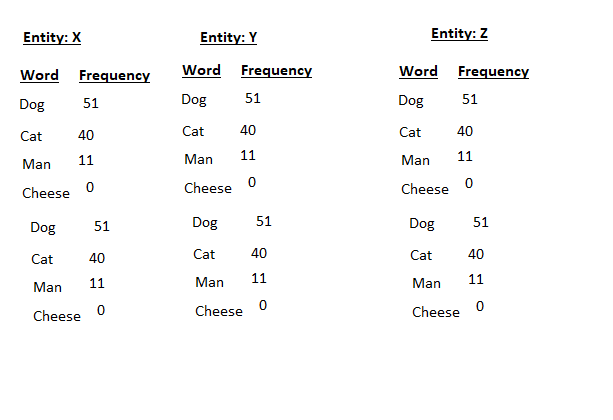
\includegraphics[width=\textwidth]{images/bowbowbow.png}
%	\centering
%	\caption{Bag-of-words  }\label{Bag-of-words-example}
%\end{figure}


 %Below, we show a review with its associated properties labelled.

%\begin{figure}[t]
%	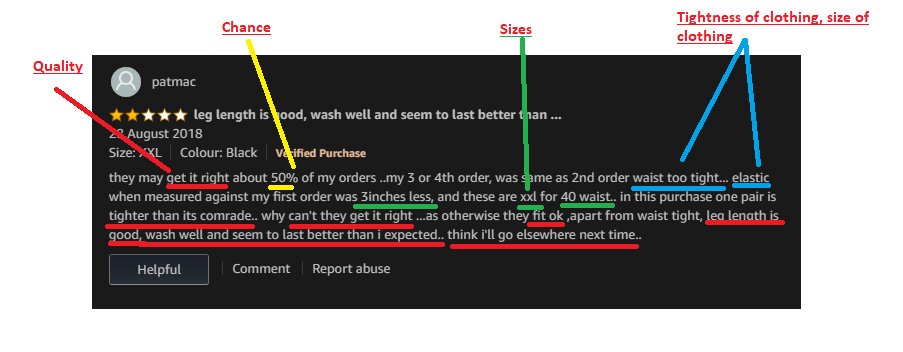
\includegraphics[width=\textwidth]{images/leg_length.png}
%	\centering
%	\caption{Example properties  }\label{IntroDecisionTree}
%\end{figure}

%\subsection{Machine Learning}
% what is machine learning? why do i care?


% Granular
%We can understand these properties to have a degree to which they apply, for example the size of the clothing might be "XXL", "XL", "L", "M" or "S", or the quality may be "Very good", "Good", "Ok", "Bad" or "Very bad". For the former, we may rely on the metadata available from the site itself, but for the latter the way to obtain this information is less clear. Although we may infer that the rating has some indication of these properties, it does not describe the properties or the degree to which the review refers to them. %This kind of information is valuable for making sense of the world of unstructured text, and has broad applications, e.g. The most immediate example is perhaps that they allow for a natural way to implement critique-based recommendation systems, where users can specify how their desired result should relate to a given set of suggestions \cite{viappiani2006preference}. For instance, \cite{Vig:2012:TGE:2362394.2362395} propose a movie recommendation system in which the user can specify that they want to see suggestions for movies that are ``similar to this one, but scarier''. If the property of being scary is adequately modelled as a direction in a semantic space of movies, such critiques can be addressed in a straightforward way. Similarly, in \cite{kovashka2012whittlesearch} a system was developed that can find ``shoes like these but shinier'', based on a semantic space representation that was derived from visual features. Semantic search systems can use such directions to interpret queries involving gradual and possibly ill-defined features, such as ``\emph{popular} holiday destinations in Europe'' \cite{DBLP:conf/sigir/JameelBS17}. While features such as popularity are typically not encoded in traditional knowledge bases, they can often be represented as semantic space directions.  %Copied from CONLL

%\subsection{Directions}\label{intro:directions}


%However, manually labelling these properties and the degrees to which entities (e.g. reviews, text-posts) have them is extremely time-consuming. 

%A potentially ideal system would be as follows: We collect large amounts of unstructured text data, separated into domains, and obtain the properties of each domain from this data, and rank entities on the degree to which they have these properties. In this way, properties would be understood on a scale built from the domain directly, so that each domain has its own meanings for words according to their own idiosyncrasies. As the process does not require any manual labelling the quality of these properties could be improved simply by obtaining more data. Further, as we are learning from unstructured data, not only would this allow us to understand the data in terms of what we know, but it would also introduce us to new ideas that we may not have previously understood. This kind of representation also has value in application to Machine Learning tasks. If we can separate the semantics of the space linearly into properties, we are able to learn simple linear classifiers that perform well. 

%Simple linear classifiers built from a representation composed of rankings on properties have an additional benefit of being more understandable.


% Natural clustering
% Semantically distinct
% Interpretable
% Curse of dimensionality
% Generalizability ("shared factors across many tasks" \cite{Bengio2012})

%What is machine learning? What are its advantages? How is it motivating?

%What are the problems with machine learning? How is it motivating?


%What is domain-specific? What is domain knowledge? %On the web there is a large volume of raw text data, e.g. Reviews of products, movies, anime, books, music, social posts by individuals, self-descriptive text about a website or product, and so on. These can be categorized into domains; each domain has its own quirks, knowledge, and method of being brought about. Although a movie review may sound similar to a book review, they typically differ hugely in the distribution of words used.

%

%\section{Interpretability}\label{ch1:interpret}

%What is interpretability? How is the value of interpretability measured in the real world?

%How can we meet the needs of the real world?  Is it transparancy, the system having easy to understnad components, etc... what  are the different views on what an interpretabile system is?

%What specific interpretability task are we trying to solve? How do we define interpretability? Why is it valuable, where is it used? What was the hypothesis/research question?
%%What are distributional models?
%Most successful approaches in recent times, like vector-spaces, word-vectors, and others, rely on the distributional model of semantics. This model relies on encoding unstructured text e.g. of a movie review, as a vector, where each dimension corresponds to how frequent each word is, we are able to calculate how similar the entities are, e.g. we know that if two movies have a similar distribution of words in their reviews, like frequent use of the word 'scary', or 'horror', then they would have a higher similarity value. These models, also known as 'semantic spaces' encode this similarity information spatially.

%Semantic relationships can be obtained from semantic spaces. 

%applications/need for good interpretability:

%What is a conceptual space? What are entities?  What are properties? What is commonsense reasoning?
%properties of an interpretable classifier:
%\begin{itemize}
%	\item Complexity: 'the magic number is seven plus or minus two' \cite{Saaty2003} also has many positive effects for its users, like lower response times \cite{Narayanan2018, Huysmans2011}, better question answering and confidence for logical problem questions \cite{Huysmans2011} and higher satisfaction \cite{Narayanan2018}.
%	\item Transparancy: 
%	\item Explainability: 
%	\item Generalizability:
%\end{itemize}


%X%X%What is a symbolic approach?  %One approach to making sense of these domains is to produce rules from expert knowledge. An expert in movies would tell you that if the review talks about it being a "cannibal horror film", we can understand that it is likely a scary movie and is related to the original 'Cannibal Holocaust' movie. Encoding this kind of knowledge is difficult, time-consuming, and hard to automate reliably.

%Properties, entities, the benefits and application of a representation formed of these

%Basic introduction to directions, explanation of the utility and application of our approach
%\section{Thesis Overview / Contributions}

%What were our objectives starting out? 
%What are our intentions with how the work in the thesis will be used?
%What are our contributions?
%%What are our aims for this chapter? What do we overall want to do? (Already kind-of said in Chapter 1, but worth repeating I guess in some form)
%In \ref{Chapter3}, we introduce a pipeline that starts with unstructured text, and ends with an interpretable representation of entities represented by properties labelled by clusters of words. Further, we demonstrate the applicability of these representations in a simple Decision Tree that uses just a few of these properties to classify entities. In Figure \ref{ExamplesWithTree}, we show some example movie entities, their associated properties, and a Decision Tree classifying whether or not they are a Horror movie. 


\backmatter 

\bibliographystyle{plain}
\bibliography{bibliography}


\end{document}
